\documentclass{book}
\usepackage[a4paper,top=2.5cm,bottom=2.5cm,left=2.5cm,right=2.5cm]{geometry}
\usepackage{makeidx}
\usepackage{natbib}
\usepackage{graphicx}
\usepackage{multicol}
\usepackage{float}
\usepackage{listings}
\usepackage{color}
\usepackage{ifthen}
\usepackage[table]{xcolor}
\usepackage{textcomp}
\usepackage{alltt}
\usepackage{ifpdf}
\ifpdf
\usepackage[pdftex,
            pagebackref=true,
            colorlinks=true,
            linkcolor=blue,
            unicode
           ]{hyperref}
\else
\usepackage[ps2pdf,
            pagebackref=true,
            colorlinks=true,
            linkcolor=blue,
            unicode
           ]{hyperref}
\usepackage{pspicture}
\fi
\usepackage[utf8]{inputenc}
\usepackage{mathptmx}
\usepackage[scaled=.90]{helvet}
\usepackage{courier}
\usepackage{sectsty}
\usepackage{amssymb}
\usepackage[titles]{tocloft}
\usepackage{doxygen}
\lstset{language=C++,inputencoding=utf8,basicstyle=\footnotesize,breaklines=true,breakatwhitespace=true,tabsize=4,numbers=left }
\makeindex
\setcounter{tocdepth}{3}
\renewcommand{\footrulewidth}{0.4pt}
\renewcommand{\familydefault}{\sfdefault}
\hfuzz=15pt
\setlength{\emergencystretch}{15pt}
\hbadness=750
\tolerance=750
\begin{document}
\hypersetup{pageanchor=false,citecolor=blue}
\begin{titlepage}
\vspace*{7cm}
\begin{center}
{\Large Com\-P\-W\-A }\\
\vspace*{1cm}
{\large Generated by Doxygen 1.8.3.1}\\
\vspace*{0.5cm}
{\small Thu Oct 24 2013 13:58:25}\\
\end{center}
\end{titlepage}
\clearemptydoublepage
\pagenumbering{roman}
\tableofcontents
\clearemptydoublepage
\pagenumbering{arabic}
\hypersetup{pageanchor=true,citecolor=blue}
\chapter{Hierarchical Index}
\section{Class Hierarchy}
This inheritance list is sorted roughly, but not completely, alphabetically:\begin{DoxyCompactList}
\item \contentsline{section}{DIFBase}{\pageref{d9/db5/classDIFBase}}{}
\begin{DoxyCompactList}
\item \contentsline{section}{DIFRootReader}{\pageref{dc/ddc/classDIFRootReader}}{}
\end{DoxyCompactList}
\item \contentsline{section}{GArgumentParser}{\pageref{d0/d39/classGArgumentParser}}{}
\item \contentsline{section}{Gem::Geneva::GStartIndividual}{\pageref{dd/d14/classGem_1_1Geneva_1_1GStartIndividual}}{}
\item \contentsline{section}{GStartIndividual}{\pageref{dd/d33/classGStartIndividual}}{}
\item \contentsline{section}{OIFBase}{\pageref{d0/d31/classOIFBase}}{}
\begin{DoxyCompactList}
\item \contentsline{section}{OIFGeneva}{\pageref{d4/dce/classOIFGeneva}}{}
\item \contentsline{section}{OIFMinuit}{\pageref{d5/db7/classOIFMinuit}}{}
\end{DoxyCompactList}
\item \contentsline{section}{OIFData}{\pageref{d1/d4f/classOIFData}}{}
\begin{DoxyCompactList}
\item \contentsline{section}{EIFBase}{\pageref{df/d13/classEIFBase}}{}
\begin{DoxyCompactList}
\item \contentsline{section}{EIFChiOneD}{\pageref{db/d1d/classEIFChiOneD}}{}
\end{DoxyCompactList}
\item \contentsline{section}{PolyFit}{\pageref{de/d89/classPolyFit}}{}
\end{DoxyCompactList}
\item \contentsline{section}{OIFMinuitFcn}{\pageref{d5/d19/classOIFMinuitFcn}}{}
\item \contentsline{section}{ROOT::Minuit2::OIFMinuitFcn}{\pageref{d3/dc7/classROOT_1_1Minuit2_1_1OIFMinuitFcn}}{}
\item \contentsline{section}{PIFBase}{\pageref{d5/d3f/classPIFBase}}{}
\begin{DoxyCompactList}
\item \contentsline{section}{PIFBW}{\pageref{d8/d58/classPIFBW}}{}
\end{DoxyCompactList}
\item \contentsline{section}{PWAEvent}{\pageref{dc/d66/classPWAEvent}}{}
\item \contentsline{section}{PWAParameter$<$ T $>$}{\pageref{d2/d41/classPWAParameter}}{}
\item \contentsline{section}{PWAParticle}{\pageref{d9/dcb/classPWAParticle}}{}
\end{DoxyCompactList}

\chapter{Data Structure Index}
\section{Class List}
Here are the classes, structs, unions and interfaces with brief descriptions:\begin{DoxyCompactList}
\item\contentsline{section}{\hyperlink{classDIFBase}{DIFBase} (Data Interface Base-\/Class )}{\pageref{d9/db5/classDIFBase}}{}
\item\contentsline{section}{\hyperlink{classDIFRootReader}{DIFRootReader} (Reader for data in Root-\/files )}{\pageref{dc/ddc/classDIFRootReader}}{}
\item\contentsline{section}{\hyperlink{classEIFBase}{EIFBase} (Estimator Interface Base-\/Class )}{\pageref{df/d13/classEIFBase}}{}
\item\contentsline{section}{\hyperlink{classEIFChiOneD}{EIFChiOneD} (Simple $\chi^{2}$-\/Estimator )}{\pageref{db/d1d/classEIFChiOneD}}{}
\item\contentsline{section}{\hyperlink{classGArgumentParser}{GArgumentParser} (Geneva Argument Parser )}{\pageref{d0/d39/classGArgumentParser}}{}
\item\contentsline{section}{\hyperlink{classGStartIndividual}{GStartIndividual} (Geneva individual for optimization )}{\pageref{dd/d33/classGStartIndividual}}{}
\item\contentsline{section}{\hyperlink{classGem_1_1Geneva_1_1GStartIndividual}{Gem::Geneva::GStartIndividual} }{\pageref{dd/d14/classGem_1_1Geneva_1_1GStartIndividual}}{}
\item\contentsline{section}{\hyperlink{classOIFBase}{OIFBase} (Optimizer Interface Base-\/Class )}{\pageref{d0/d31/classOIFBase}}{}
\item\contentsline{section}{\hyperlink{classOIFData}{OIFData} (Optimizer Data Base-\/Class )}{\pageref{d1/d4f/classOIFData}}{}
\item\contentsline{section}{\hyperlink{classOIFGeneva}{OIFGeneva} (Wrapper of the Geneva Optimizer library )}{\pageref{d4/dce/classOIFGeneva}}{}
\item\contentsline{section}{\hyperlink{classOIFMinuit}{OIFMinuit} (Wrapper of the Minuit2 Optimizer library )}{\pageref{d5/db7/classOIFMinuit}}{}
\item\contentsline{section}{\hyperlink{classOIFMinuitFcn}{OIFMinuitFcn} (Minuit2 function to be optimized )}{\pageref{d5/d19/classOIFMinuitFcn}}{}
\item\contentsline{section}{\hyperlink{classROOT_1_1Minuit2_1_1OIFMinuitFcn}{ROOT::Minuit2::OIFMinuitFcn} }{\pageref{d3/dc7/classROOT_1_1Minuit2_1_1OIFMinuitFcn}}{}
\item\contentsline{section}{\hyperlink{classPIFBase}{PIFBase} (Physics Interface Base-\/Class )}{\pageref{d5/d3f/classPIFBase}}{}
\item\contentsline{section}{\hyperlink{classPIFBW}{PIFBW} (Physics Module with simple 1D Breit-\/Wigner )}{\pageref{d8/d58/classPIFBW}}{}
\item\contentsline{section}{\hyperlink{classPolyFit}{PolyFit} (Test implementation of \hyperlink{OIFData_8hpp}{OIFData.hpp} )}{\pageref{de/d89/classPolyFit}}{}
\item\contentsline{section}{\hyperlink{classPWAEvent}{PWAEvent} (Internal container for event information )}{\pageref{dc/d66/classPWAEvent}}{}
\item\contentsline{section}{\hyperlink{classPWAParticle}{PWAParticle} (Internal container representing a particle )}{\pageref{d9/dcb/classPWAParticle}}{}
\end{DoxyCompactList}

\chapter{File Index}
\section{File List}
Here is a list of all files with brief descriptions:\begin{DoxyCompactList}
\item\contentsline{section}{Core/\hyperlink{DIFBase_8hpp}{DIFBase.hpp} (This class provides the interface to experimental data )}{\pageref{db/d2c/DIFBase_8hpp}}{}
\item\contentsline{section}{Core/\hyperlink{EIFBase_8hpp}{EIFBase.hpp} (This class provides the interface to classes which estimate the \char`\"{}closeness\char`\"{} of the modeled intensity to the data )}{\pageref{df/d05/EIFBase_8hpp}}{}
\item\contentsline{section}{Core/\hyperlink{OIFBase_8hpp}{OIFBase.hpp} (This class provides the interface to (external) optimization libraries or routines )}{\pageref{d8/dc8/OIFBase_8hpp}}{}
\item\contentsline{section}{Core/\hyperlink{OIFData_8hpp}{OIFData.hpp} (This class provides the interface for the optimizer module to access the data )}{\pageref{db/dc2/OIFData_8hpp}}{}
\item\contentsline{section}{Core/\hyperlink{PIFBase_8hpp}{PIFBase.hpp} (This class provides the interface to the model which tries to describe the intensity )}{\pageref{de/dc5/PIFBase_8hpp}}{}
\item\contentsline{section}{Core/\hyperlink{PWAEvent_8hpp}{PWAEvent.hpp} (This class provides a internal container for event-\/based information )}{\pageref{d8/d14/PWAEvent_8hpp}}{}
\item\contentsline{section}{Core/\hyperlink{PWAParticle_8hpp}{PWAParticle.hpp} (This class provides a internal container for information of a particle )}{\pageref{d3/ded/PWAParticle_8hpp}}{}
\item\contentsline{section}{DIFRoot2Part/\hyperlink{DIFRootReader_8cpp}{DIFRootReader.cpp} }{\pageref{dd/de5/DIFRootReader_8cpp}}{}
\item\contentsline{section}{DIFRoot2Part/\hyperlink{DIFRootReader_8hpp}{DIFRootReader.hpp} (This class reads event-\/based data from root-\/files )}{\pageref{db/d3e/DIFRootReader_8hpp}}{}
\item\contentsline{section}{EIFChiOneD/\hyperlink{EIFChiOneD_8cpp}{EIFChiOneD.cpp} }{\pageref{d8/d80/EIFChiOneD_8cpp}}{}
\item\contentsline{section}{EIFChiOneD/\hyperlink{EIFChiOneD_8hpp}{EIFChiOneD.hpp} (This class calculates a simple $\chi^{2}$ of a intensity and a dataset )}{\pageref{d3/d5d/EIFChiOneD_8hpp}}{}
\item\contentsline{section}{OIFGeneva/\hyperlink{GArgumentParser_8cpp}{GArgumentParser.cpp} }{\pageref{d5/d42/GArgumentParser_8cpp}}{}
\item\contentsline{section}{OIFGeneva/\hyperlink{GArgumentParser_8hpp}{GArgumentParser.hpp} (Geneva argument parser to interpret command line arguments and config files )}{\pageref{d4/d3c/GArgumentParser_8hpp}}{}
\item\contentsline{section}{OIFGeneva/\hyperlink{GStartIndividual_8hpp}{GStartIndividual.hpp} (Geneva individual extended to the use in ComPWA, using \hyperlink{classOIFData}{OIFData} to access the data )}{\pageref{df/dfa/GStartIndividual_8hpp}}{}
\item\contentsline{section}{OIFGeneva/\hyperlink{OIFGeneva_8cpp}{OIFGeneva.cpp} }{\pageref{dc/ddb/OIFGeneva_8cpp}}{}
\item\contentsline{section}{OIFGeneva/\hyperlink{OIFGeneva_8hpp}{OIFGeneva.hpp} (This class provides a wrapper around the Geneva library )}{\pageref{d2/dcf/OIFGeneva_8hpp}}{}
\item\contentsline{section}{OIFMinuit2/\hyperlink{OIFMinuit_8cpp}{OIFMinuit.cpp} }{\pageref{d7/d2d/OIFMinuit_8cpp}}{}
\item\contentsline{section}{OIFMinuit2/\hyperlink{OIFMinuit_8hpp}{OIFMinuit.hpp} (This class provides a wrapper around the Minuit2 library )}{\pageref{d8/d0f/OIFMinuit_8hpp}}{}
\item\contentsline{section}{OIFMinuit2/\hyperlink{OIFMinuitFcn_8cpp}{OIFMinuitFcn.cpp} }{\pageref{d5/db0/OIFMinuitFcn_8cpp}}{}
\item\contentsline{section}{OIFMinuit2/\hyperlink{OIFMinuitFcn_8hpp}{OIFMinuitFcn.hpp} (Based on the Minuit2 FcnBase )}{\pageref{d4/dce/OIFMinuitFcn_8hpp}}{}
\item\contentsline{section}{PIFBW/\hyperlink{PIFBW_8cpp}{PIFBW.cpp} }{\pageref{d5/dbb/PIFBW_8cpp}}{}
\item\contentsline{section}{PIFBW/\hyperlink{PIFBW_8hpp}{PIFBW.hpp} (This class provides a simple Breit-\/Wigner calculation with given parameters )}{\pageref{dd/da0/PIFBW_8hpp}}{}
\item\contentsline{section}{test/\hyperlink{CX0TestApp_8cpp}{CX0TestApp.cpp} (Test-\/Application to check c++11 support )}{\pageref{d5/d7b/CX0TestApp_8cpp}}{}
\item\contentsline{section}{test/\hyperlink{DataIFTestApp_8cpp}{DataIFTestApp.cpp} (Test-\/Application of the Root Data-\/IF )}{\pageref{db/d8a/DataIFTestApp_8cpp}}{}
\item\contentsline{section}{test/\hyperlink{EstimatorTestApp_8cpp}{EstimatorTestApp.cpp} (Test-\/Application of a simple $\chi^{2}$ estimator )}{\pageref{d4/d31/EstimatorTestApp_8cpp}}{}
\item\contentsline{section}{test/\hyperlink{MinuitTestApp_8cpp}{MinuitTestApp.cpp} (Test-\/Application of the Minuit2 Optimizer-\/IF )}{\pageref{da/d21/MinuitTestApp_8cpp}}{}
\item\contentsline{section}{test/\hyperlink{OptimizerTestApp_8cpp}{OptimizerTestApp.cpp} (Test-\/Application of the Optimizer-\/IF )}{\pageref{d4/db7/OptimizerTestApp_8cpp}}{}
\item\contentsline{section}{test/\hyperlink{PhysicsTestApp_8cpp}{PhysicsTestApp.cpp} (Test-\/Application of the Physics-\/IF )}{\pageref{db/da0/PhysicsTestApp_8cpp}}{}
\item\contentsline{section}{test/\hyperlink{PolyFit_8cpp}{PolyFit.cpp} }{\pageref{d5/d8b/PolyFit_8cpp}}{}
\item\contentsline{section}{test/\hyperlink{PolyFit_8hpp}{PolyFit.hpp} (This class derives from \hyperlink{OIFData_8hpp}{OIFData.hpp}, the data-\/interface of the optimizers )}{\pageref{d2/dcb/PolyFit_8hpp}}{}
\end{DoxyCompactList}

\chapter{Data Structure Documentation}
\hypertarget{class_amp_abs_dynamical_function}{\section{Amp\-Abs\-Dynamical\-Function Class Reference}
\label{class_amp_abs_dynamical_function}\index{Amp\-Abs\-Dynamical\-Function@{Amp\-Abs\-Dynamical\-Function}}
}
Inheritance diagram for Amp\-Abs\-Dynamical\-Function\-:\begin{figure}[H]
\begin{center}
\leavevmode
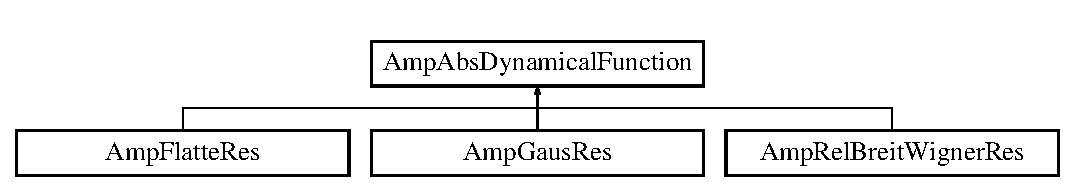
\includegraphics[height=2.000000cm]{class_amp_abs_dynamical_function}
\end{center}
\end{figure}
\subsection*{Public Member Functions}
\begin{DoxyCompactItemize}
\item 
\hypertarget{class_amp_abs_dynamical_function_a28bc08161eec1480e2c52d91ec8c5be8}{{\bfseries Amp\-Abs\-Dynamical\-Function} (const char $\ast$name)}\label{class_amp_abs_dynamical_function_a28bc08161eec1480e2c52d91ec8c5be8}

\item 
\hypertarget{class_amp_abs_dynamical_function_a13ca78b1eaa2998c3db8c3eca8c93bac}{{\bfseries Amp\-Abs\-Dynamical\-Function} (const \hyperlink{class_amp_abs_dynamical_function}{Amp\-Abs\-Dynamical\-Function} \&, const char $\ast$)}\label{class_amp_abs_dynamical_function_a13ca78b1eaa2998c3db8c3eca8c93bac}

\item 
\hypertarget{class_amp_abs_dynamical_function_a7ba5980ea098ed83d96a9c6464c8bb6a}{virtual void {\bfseries initialise} ()=0}\label{class_amp_abs_dynamical_function_a7ba5980ea098ed83d96a9c6464c8bb6a}

\item 
\hypertarget{class_amp_abs_dynamical_function_a1fafdad84744aa1469e4696030598084}{virtual std\-::complex$<$ double $>$ {\bfseries evaluate} () const =0}\label{class_amp_abs_dynamical_function_a1fafdad84744aa1469e4696030598084}

\item 
\hypertarget{class_amp_abs_dynamical_function_a89b4fafcd8421366b5f923fd0e12de30}{virtual double {\bfseries get\-Spin} ()=0}\label{class_amp_abs_dynamical_function_a89b4fafcd8421366b5f923fd0e12de30}

\item 
\hypertarget{class_amp_abs_dynamical_function_a6bf35600e519ab9e257b978275dd4297}{virtual bool {\bfseries is\-Sub\-Sys} (const unsigned int) const =0}\label{class_amp_abs_dynamical_function_a6bf35600e519ab9e257b978275dd4297}

\item 
\hypertarget{class_amp_abs_dynamical_function_a3b9b4feba0885d42fd823d2a84f41b81}{virtual double {\bfseries integral} () const =0}\label{class_amp_abs_dynamical_function_a3b9b4feba0885d42fd823d2a84f41b81}

\item 
\hypertarget{class_amp_abs_dynamical_function_a9ec34f0d8d6d0526d171358fb267a7fd}{virtual std\-::string {\bfseries Get\-Name} ()}\label{class_amp_abs_dynamical_function_a9ec34f0d8d6d0526d171358fb267a7fd}

\item 
\hypertarget{class_amp_abs_dynamical_function_ac181b0715993d90867b78b392c2e0be9}{virtual std\-::string {\bfseries Get\-Title} ()}\label{class_amp_abs_dynamical_function_ac181b0715993d90867b78b392c2e0be9}

\end{DoxyCompactItemize}
\subsection*{Protected Attributes}
\begin{DoxyCompactItemize}
\item 
\hypertarget{class_amp_abs_dynamical_function_aa7c6f2ca7dafa5c9af7e9a7af77a0df1}{std\-::string {\bfseries \-\_\-name}}\label{class_amp_abs_dynamical_function_aa7c6f2ca7dafa5c9af7e9a7af77a0df1}

\end{DoxyCompactItemize}


The documentation for this class was generated from the following files\-:\begin{DoxyCompactItemize}
\item 
Physics/\-Amplitude\-Sum/Amp\-Abs\-Dynamical\-Function.\-hpp\item 
Physics/\-Amplitude\-Sum/Amp\-Abs\-Dynamical\-Function.\-cpp\end{DoxyCompactItemize}

\hypertarget{class_amp_fcn}{\section{Amp\-Fcn Class Reference}
\label{class_amp_fcn}\index{Amp\-Fcn@{Amp\-Fcn}}
}
Inheritance diagram for Amp\-Fcn\-:\begin{figure}[H]
\begin{center}
\leavevmode
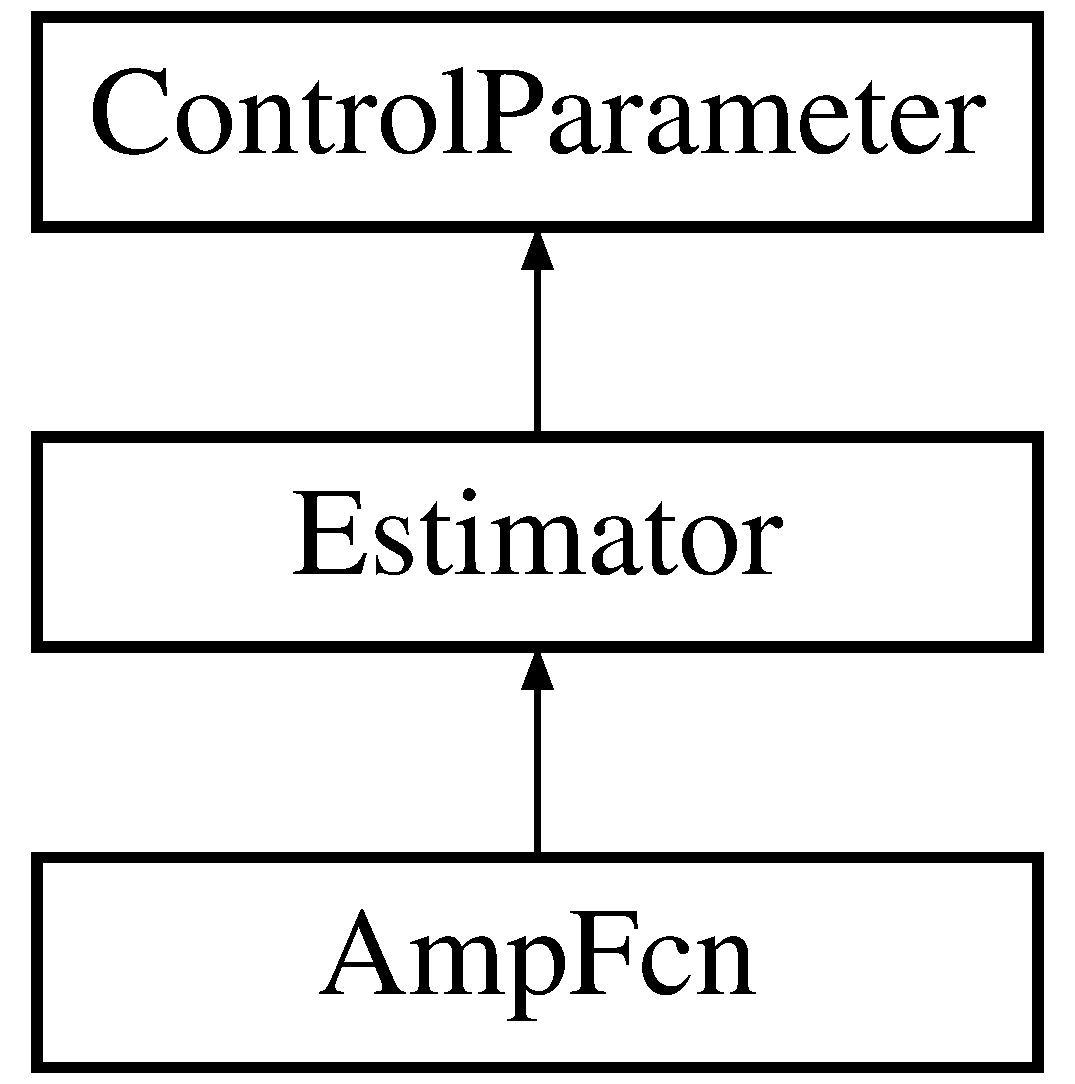
\includegraphics[height=3.000000cm]{class_amp_fcn}
\end{center}
\end{figure}
\subsection*{Public Member Functions}
\begin{DoxyCompactItemize}
\item 
\hypertarget{class_amp_fcn_ac195a8261ff78dd0c9b526734ca94f62}{{\bfseries Amp\-Fcn} (\hyperlink{class_amplitude}{Amplitude} $\ast$amp)}\label{class_amp_fcn_ac195a8261ff78dd0c9b526734ca94f62}

\item 
\hypertarget{class_amp_fcn_a9bb2555dd3762ed399e12e3526d9b316}{virtual double {\bfseries control\-Parameter} (\hyperlink{class_parameter_list}{Parameter\-List} \&x)}\label{class_amp_fcn_a9bb2555dd3762ed399e12e3526d9b316}

\end{DoxyCompactItemize}
\subsection*{Additional Inherited Members}


The documentation for this class was generated from the following file\-:\begin{DoxyCompactItemize}
\item 
Estimator/Amp\-Fcn.\-cpp\end{DoxyCompactItemize}

\hypertarget{class_amp_flatte_res}{\section{Amp\-Flatte\-Res Class Reference}
\label{class_amp_flatte_res}\index{Amp\-Flatte\-Res@{Amp\-Flatte\-Res}}
}
Inheritance diagram for Amp\-Flatte\-Res\-:\begin{figure}[H]
\begin{center}
\leavevmode
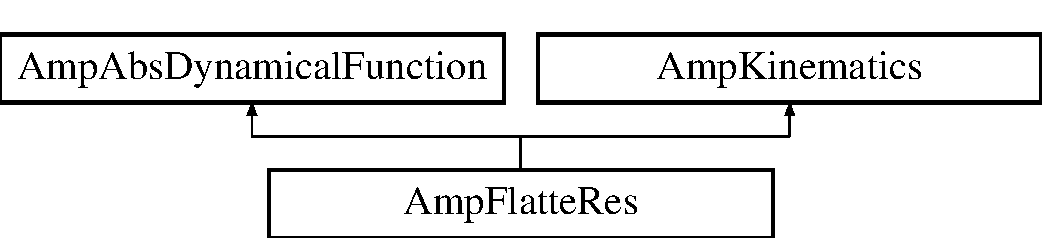
\includegraphics[height=2.000000cm]{class_amp_flatte_res}
\end{center}
\end{figure}
\subsection*{Public Member Functions}
\begin{DoxyCompactItemize}
\item 
\hyperlink{class_amp_flatte_res_ac3fe9d6623c886a1d830d1096cf488bb}{Amp\-Flatte\-Res} (const char $\ast$name, \hyperlink{class_double_parameter}{Double\-Parameter} \&res\-Mass, \hyperlink{class_double_parameter}{Double\-Parameter} \&res\-Width, double \&meson\-Radius, \hyperlink{class_double_parameter}{Double\-Parameter} \&coupling\-Hidden, \hyperlink{class_double_parameter}{Double\-Parameter} \&coupling, double \-\_\-mass\-Hidden\-Channel\-A, double \-\_\-mass\-Hidden\-Channel\-B, int \-\_\-subsys, int res\-Spin, int m, int n)
\item 
\hypertarget{class_amp_flatte_res_a39f722458936723ff3a92e70b2a1a1c6}{{\bfseries Amp\-Flatte\-Res} (const \hyperlink{class_amp_flatte_res}{Amp\-Flatte\-Res} \&, const char $\ast$)}\label{class_amp_flatte_res_a39f722458936723ff3a92e70b2a1a1c6}

\item 
\hypertarget{class_amp_flatte_res_abfcd5665519217946d69f89e77359211}{{\bfseries Amp\-Flatte\-Res} (const \hyperlink{class_amp_flatte_res}{Amp\-Flatte\-Res} \&)}\label{class_amp_flatte_res_abfcd5665519217946d69f89e77359211}

\item 
\hypertarget{class_amp_flatte_res_aceb105ba7f489aeceb2bfd173da0d814}{void {\bfseries set\-Barrier\-Mass} (double, double)}\label{class_amp_flatte_res_aceb105ba7f489aeceb2bfd173da0d814}

\item 
\hypertarget{class_amp_flatte_res_a73a7e85ab72937d88b7972f43dcfee6e}{virtual void {\bfseries initialise} ()}\label{class_amp_flatte_res_a73a7e85ab72937d88b7972f43dcfee6e}

\item 
\hypertarget{class_amp_flatte_res_a3ec6caa50a53820e4f3074a72091882b}{virtual std\-::complex$<$ double $>$ {\bfseries evaluate} () const }\label{class_amp_flatte_res_a3ec6caa50a53820e4f3074a72091882b}

\item 
\hypertarget{class_amp_flatte_res_adf81c0acd73732e33021e218f422a4d7}{void {\bfseries set\-Decay\-Masses} (double, double, double, double)}\label{class_amp_flatte_res_adf81c0acd73732e33021e218f422a4d7}

\item 
\hypertarget{class_amp_flatte_res_ae3226ffa36fab59f58739301c806eddc}{double {\bfseries integral} () const }\label{class_amp_flatte_res_ae3226ffa36fab59f58739301c806eddc}

\item 
\hypertarget{class_amp_flatte_res_af1f4f764b8d9bc3ecf0885d2c0bc8a16}{double {\bfseries get\-Spin} ()}\label{class_amp_flatte_res_af1f4f764b8d9bc3ecf0885d2c0bc8a16}

\item 
\hypertarget{class_amp_flatte_res_a84a21d076a16bd561050636f1a11d2d8}{virtual bool {\bfseries is\-Sub\-Sys} (const unsigned int sub\-Sys) const }\label{class_amp_flatte_res_a84a21d076a16bd561050636f1a11d2d8}

\end{DoxyCompactItemize}
\subsection*{Protected Attributes}
\begin{DoxyCompactItemize}
\item 
\hypertarget{class_amp_flatte_res_a4028cf958cef457c7b286d22b03cab86}{\hyperlink{class_double_parameter}{Double\-Parameter} {\bfseries \-\_\-coupling\-Hidden\-Channel}}\label{class_amp_flatte_res_a4028cf958cef457c7b286d22b03cab86}

\item 
\hypertarget{class_amp_flatte_res_a5675c0fdb0369784d1a3b01f9472f1a0}{\hyperlink{class_double_parameter}{Double\-Parameter} {\bfseries \-\_\-coupling}}\label{class_amp_flatte_res_a5675c0fdb0369784d1a3b01f9472f1a0}

\item 
\hypertarget{class_amp_flatte_res_a8abf0ba653dbc494518ca670450de6b6}{\hyperlink{class_amp_wigner}{Amp\-Wigner} {\bfseries \-\_\-wigner\-D}}\label{class_amp_flatte_res_a8abf0ba653dbc494518ca670450de6b6}

\item 
\hypertarget{class_amp_flatte_res_abc484aa206565bfca140ac1d12d57172}{double {\bfseries \-\_\-mass\-Hidden\-Channel\-B}}\label{class_amp_flatte_res_abc484aa206565bfca140ac1d12d57172}

\item 
\hypertarget{class_amp_flatte_res_a95dcabbe9c00c916427b8d1efc0dadee}{double {\bfseries \-\_\-mass\-Hidden\-Channel\-A}}\label{class_amp_flatte_res_a95dcabbe9c00c916427b8d1efc0dadee}

\end{DoxyCompactItemize}
\subsection*{Additional Inherited Members}


\subsection{Constructor \& Destructor Documentation}
\hypertarget{class_amp_flatte_res_ac3fe9d6623c886a1d830d1096cf488bb}{\index{Amp\-Flatte\-Res@{Amp\-Flatte\-Res}!Amp\-Flatte\-Res@{Amp\-Flatte\-Res}}
\index{Amp\-Flatte\-Res@{Amp\-Flatte\-Res}!AmpFlatteRes@{Amp\-Flatte\-Res}}
\subsubsection[{Amp\-Flatte\-Res}]{\setlength{\rightskip}{0pt plus 5cm}Amp\-Flatte\-Res\-::\-Amp\-Flatte\-Res (
\begin{DoxyParamCaption}
\item[{const char $\ast$}]{name, }
\item[{{\bf Double\-Parameter} \&}]{res\-Mass, }
\item[{{\bf Double\-Parameter} \&}]{res\-Width, }
\item[{double \&}]{meson\-Radius, }
\item[{{\bf Double\-Parameter} \&}]{coupling\-Hidden, }
\item[{{\bf Double\-Parameter} \&}]{coupling, }
\item[{double}]{\-\_\-mass\-Hidden\-Channel\-A, }
\item[{double}]{\-\_\-mass\-Hidden\-Channel\-B, }
\item[{int}]{\-\_\-subsys, }
\item[{int}]{res\-Spin, }
\item[{int}]{m, }
\item[{int}]{n}
\end{DoxyParamCaption}
)}}\label{class_amp_flatte_res_ac3fe9d6623c886a1d830d1096cf488bb}

\begin{DoxyParams}{Parameters}
{\em coupling\-Hidden} & meson radius \\
\hline
{\em res\-Spin} & meson radius \\
\hline
\end{DoxyParams}


The documentation for this class was generated from the following files\-:\begin{DoxyCompactItemize}
\item 
Physics/\-Amplitude\-Sum/Amp\-Flatte\-Res.\-hpp\item 
Physics/\-Amplitude\-Sum/Amp\-Flatte\-Res.\-cpp\end{DoxyCompactItemize}

\hypertarget{class_amp_gaus_res}{\section{Amp\-Gaus\-Res Class Reference}
\label{class_amp_gaus_res}\index{Amp\-Gaus\-Res@{Amp\-Gaus\-Res}}
}
Inheritance diagram for Amp\-Gaus\-Res\-:\begin{figure}[H]
\begin{center}
\leavevmode
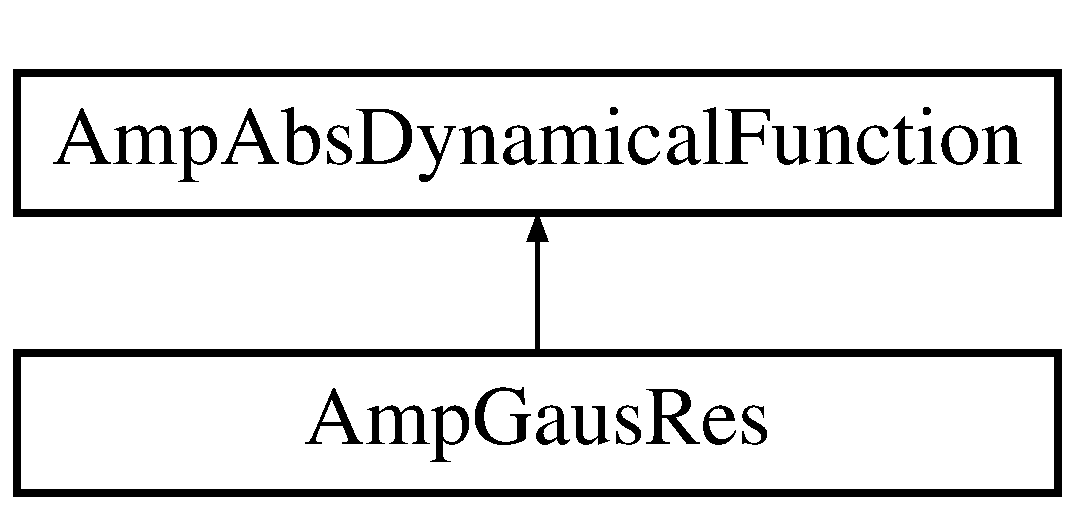
\includegraphics[height=2.000000cm]{class_amp_gaus_res}
\end{center}
\end{figure}
\subsection*{Public Member Functions}
\begin{DoxyCompactItemize}
\item 
\hypertarget{class_amp_gaus_res_a6557a4dd37a02f200a7fb05f182a92c1}{{\bfseries Amp\-Gaus\-Res} (const char $\ast$name, \hyperlink{class_double_parameter}{Double\-Parameter} \&\-\_\-res\-Mass, \hyperlink{class_double_parameter}{Double\-Parameter} \&\-\_\-res\-Width, int \-\_\-subsys)}\label{class_amp_gaus_res_a6557a4dd37a02f200a7fb05f182a92c1}

\item 
\hypertarget{class_amp_gaus_res_a29f81df3b1221bb8f51bb7f2e6b30bb0}{{\bfseries Amp\-Gaus\-Res} (const \hyperlink{class_amp_gaus_res}{Amp\-Gaus\-Res} \&, const char $\ast$)}\label{class_amp_gaus_res_a29f81df3b1221bb8f51bb7f2e6b30bb0}

\item 
\hypertarget{class_amp_gaus_res_a4cd1e8c23f1bb6917729ec185133a78e}{{\bfseries Amp\-Gaus\-Res} (const \hyperlink{class_amp_gaus_res}{Amp\-Gaus\-Res} \&)}\label{class_amp_gaus_res_a4cd1e8c23f1bb6917729ec185133a78e}

\item 
\hypertarget{class_amp_gaus_res_a8a8b898346b9a8a3e277a7cd3618cdee}{virtual void {\bfseries initialise} ()}\label{class_amp_gaus_res_a8a8b898346b9a8a3e277a7cd3618cdee}

\item 
\hypertarget{class_amp_gaus_res_a92183914f8fa048073f6599a56ce0cd3}{virtual std\-::complex$<$ double $>$ {\bfseries evaluate} () const }\label{class_amp_gaus_res_a92183914f8fa048073f6599a56ce0cd3}

\item 
\hypertarget{class_amp_gaus_res_aef07a6176d609572a564f37f187d24df}{virtual double {\bfseries evaluate} (double x\mbox{[}$\,$\mbox{]}, int dim, void $\ast$param) const }\label{class_amp_gaus_res_aef07a6176d609572a564f37f187d24df}

\item 
\hypertarget{class_amp_gaus_res_a328003b9ffff46daf55f747fdeb8a92d}{double {\bfseries get\-Maximum} () const }\label{class_amp_gaus_res_a328003b9ffff46daf55f747fdeb8a92d}

\item 
\hypertarget{class_amp_gaus_res_ae578a7d89933f434906dcfce7c259d60}{double {\bfseries integral} () const }\label{class_amp_gaus_res_ae578a7d89933f434906dcfce7c259d60}

\item 
\hypertarget{class_amp_gaus_res_acd7ec796cdb1c9c19a7ec3ddd0a0b68a}{virtual bool {\bfseries is\-Sub\-Sys} (const unsigned int sub\-Sys) const }\label{class_amp_gaus_res_acd7ec796cdb1c9c19a7ec3ddd0a0b68a}

\item 
\hypertarget{class_amp_gaus_res_a092845696d6be8b5b6dd78b9d5bf5fc8}{double {\bfseries get\-Spin} ()}\label{class_amp_gaus_res_a092845696d6be8b5b6dd78b9d5bf5fc8}

\end{DoxyCompactItemize}
\subsection*{Protected Attributes}
\begin{DoxyCompactItemize}
\item 
\hypertarget{class_amp_gaus_res_a7a629bcb5cc901a76582bcbf3fe4cebe}{\hyperlink{class_double_parameter}{Double\-Parameter} {\bfseries \-\_\-m\-R}}\label{class_amp_gaus_res_a7a629bcb5cc901a76582bcbf3fe4cebe}

\item 
\hypertarget{class_amp_gaus_res_a94215481ed03576aa8958070f4acfe81}{\hyperlink{class_double_parameter}{Double\-Parameter} {\bfseries \-\_\-res\-Width}}\label{class_amp_gaus_res_a94215481ed03576aa8958070f4acfe81}

\item 
\hypertarget{class_amp_gaus_res_a749db5ee2fa34cdb92c9bbda80d1ff85}{unsigned int {\bfseries \-\_\-sub\-Sys}}\label{class_amp_gaus_res_a749db5ee2fa34cdb92c9bbda80d1ff85}

\end{DoxyCompactItemize}


The documentation for this class was generated from the following files\-:\begin{DoxyCompactItemize}
\item 
Physics/\-Amplitude\-Sum/Amp\-Gaus\-Res.\-hpp\item 
Physics/\-Amplitude\-Sum/Amp\-Gaus\-Res.\-cpp\end{DoxyCompactItemize}

\hypertarget{structamp_info}{\section{amp\-Info Struct Reference}
\label{structamp_info}\index{amp\-Info@{amp\-Info}}
}
\subsection*{Public Member Functions}
\begin{DoxyCompactItemize}
\item 
\hypertarget{structamp_info_adf51b3bea0df687ae0efa95acf047aae}{{\bfseries amp\-Info} (std\-::string in\-N, std\-::shared\-\_\-ptr$<$ \hyperlink{class_amplitude}{Amplitude} $>$ in\-D, std\-::vector$<$ std\-::string $>$ in\-P)}\label{structamp_info_adf51b3bea0df687ae0efa95acf047aae}

\end{DoxyCompactItemize}
\subsection*{Data Fields}
\begin{DoxyCompactItemize}
\item 
\hypertarget{structamp_info_a0263db94bf652961389a1e4e508cac55}{std\-::string {\bfseries name}}\label{structamp_info_a0263db94bf652961389a1e4e508cac55}

\item 
\hypertarget{structamp_info_abf7aa0471429f084b02f6919ae9c577b}{std\-::shared\-\_\-ptr$<$ \hyperlink{class_amplitude}{Amplitude} $>$ {\bfseries amplitude}}\label{structamp_info_abf7aa0471429f084b02f6919ae9c577b}

\item 
\hypertarget{structamp_info_aa6921b9706ace35b8f7e9768a88aee14}{std\-::vector$<$ std\-::string $>$ {\bfseries input\-Needed}}\label{structamp_info_aa6921b9706ace35b8f7e9768a88aee14}

\end{DoxyCompactItemize}


The documentation for this struct was generated from the following file\-:\begin{DoxyCompactItemize}
\item 
Core/\hyperlink{_dictionary_8hpp}{Dictionary.\-hpp}\end{DoxyCompactItemize}

\hypertarget{class_amp_kinematics}{\section{Amp\-Kinematics Class Reference}
\label{class_amp_kinematics}\index{Amp\-Kinematics@{Amp\-Kinematics}}
}
Inheritance diagram for Amp\-Kinematics\-:\begin{figure}[H]
\begin{center}
\leavevmode
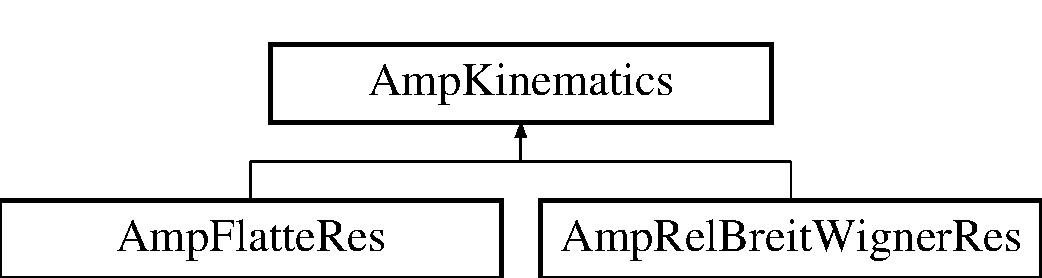
\includegraphics[height=2.000000cm]{class_amp_kinematics}
\end{center}
\end{figure}
\subsection*{Public Types}
\begin{DoxyCompactItemize}
\item 
enum {\bfseries barrier\-Type} \{ {\bfseries B\-W\-Prime}, 
{\bfseries B\-W}, 
{\bfseries none}
 \}
\end{DoxyCompactItemize}
\subsection*{Public Member Functions}
\begin{DoxyCompactItemize}
\item 
\hypertarget{class_amp_kinematics_ace5b6541a67975ab2959d9388bedafb7}{{\bfseries Amp\-Kinematics} (\hyperlink{class_double_parameter}{Double\-Parameter}, int, int, int, int, barrier\-Type, double, double)}\label{class_amp_kinematics_ace5b6541a67975ab2959d9388bedafb7}

\item 
\hypertarget{class_amp_kinematics_a7ab6c3b260a340337ff757c645f6040c}{{\bfseries Amp\-Kinematics} (double, double, double, double, \hyperlink{class_double_parameter}{Double\-Parameter}, int, barrier\-Type, int, int, int, double, double)}\label{class_amp_kinematics_a7ab6c3b260a340337ff757c645f6040c}

\item 
\hypertarget{class_amp_kinematics_a8aae4a1049a5a135370799b447f48d3c}{{\bfseries Amp\-Kinematics} (const \hyperlink{class_amp_kinematics}{Amp\-Kinematics} \&other)}\label{class_amp_kinematics_a8aae4a1049a5a135370799b447f48d3c}

\item 
\hypertarget{class_amp_kinematics_ae85be074eb945a308820f6a534e865d3}{double {\bfseries get\-E\-C\-M\-S3\-\_\-12} ()}\label{class_amp_kinematics_ae85be074eb945a308820f6a534e865d3}

\item 
\hypertarget{class_amp_kinematics_a335620a155d93949ae8f51a966e28f3c}{double {\bfseries get\-E\-C\-M\-S1\-\_\-12} ()}\label{class_amp_kinematics_a335620a155d93949ae8f51a966e28f3c}

\item 
\hypertarget{class_amp_kinematics_abe249f2dfca497bc9e0c09772dea5654}{double {\bfseries Eto\-P} (double e)}\label{class_amp_kinematics_abe249f2dfca497bc9e0c09772dea5654}

\item 
\hypertarget{class_amp_kinematics_a27f22245aeb15716c14132f97266e1be}{virtual void {\bfseries set\-Decay\-Masses} (double, double, double, double)}\label{class_amp_kinematics_a27f22245aeb15716c14132f97266e1be}

\item 
\hypertarget{class_amp_kinematics_a568842f11435e7c791806ca2dce2fd02}{void {\bfseries set\-Barrier\-Type} (int)}\label{class_amp_kinematics_a568842f11435e7c791806ca2dce2fd02}

\item 
\hypertarget{class_amp_kinematics_af2f3b8acc45052cb542e3c5b7113b53f}{void {\bfseries set\-Barrier\-Radi} (double meson\-Radius, double mother\-Radius)}\label{class_amp_kinematics_af2f3b8acc45052cb542e3c5b7113b53f}

\item 
\hypertarget{class_amp_kinematics_a2bcea6d497808708d8b4ebd45b300d29}{virtual double {\bfseries integral} () const =0}\label{class_amp_kinematics_a2bcea6d497808708d8b4ebd45b300d29}

\item 
\hypertarget{class_amp_kinematics_a8be1e6f1a1882aaf8c0a5b071fae0037}{double {\bfseries q0} (double, double) const }\label{class_amp_kinematics_a8be1e6f1a1882aaf8c0a5b071fae0037}

\item 
\hypertarget{class_amp_kinematics_a01232d768abb7a1d11a1c5f34f3de337}{double {\bfseries q0} () const }\label{class_amp_kinematics_a01232d768abb7a1d11a1c5f34f3de337}

\item 
\hypertarget{class_amp_kinematics_a35d46b91f21c11e993ca7322845b1ac0}{double {\bfseries q} (double, double, double) const }\label{class_amp_kinematics_a35d46b91f21c11e993ca7322845b1ac0}

\item 
\hypertarget{class_amp_kinematics_a5ea5cfbe70dd50fffbd151a061eb8b8a}{double {\bfseries q} (double x) const }\label{class_amp_kinematics_a5ea5cfbe70dd50fffbd151a061eb8b8a}

\item 
\hypertarget{class_amp_kinematics_a8032a5eef359956ee8ac515066eb9df0}{double {\bfseries B\-Lres2} (double x) const }\label{class_amp_kinematics_a8032a5eef359956ee8ac515066eb9df0}

\item 
\hypertarget{class_amp_kinematics_a19ccd90e265f0a413705ca8788173f7b}{double {\bfseries B\-Lmother2} (double x) const }\label{class_amp_kinematics_a19ccd90e265f0a413705ca8788173f7b}

\item 
\hypertarget{class_amp_kinematics_aeeaa97d504bc79598854a15e6566513a}{double {\bfseries get\-Res\-Mass} ()}\label{class_amp_kinematics_aeeaa97d504bc79598854a15e6566513a}

\item 
\hypertarget{class_amp_kinematics_a0a2da046c355c7f6ac473b0bdb7fa0aa}{double {\bfseries get\-M} ()}\label{class_amp_kinematics_a0a2da046c355c7f6ac473b0bdb7fa0aa}

\item 
\hypertarget{class_amp_kinematics_adccc4dcf170ea5e7ecc178fd890d5f67}{double {\bfseries get\-N} ()}\label{class_amp_kinematics_adccc4dcf170ea5e7ecc178fd890d5f67}

\item 
\hypertarget{class_amp_kinematics_a2d74e60226009affa6560f0f4611ad00}{double {\bfseries get\-Meson\-Radius} ()}\label{class_amp_kinematics_a2d74e60226009affa6560f0f4611ad00}

\item 
\hypertarget{class_amp_kinematics_a241070f8e5db82b4c36d49d8977289fe}{double {\bfseries get\-Mother\-Radius} ()}\label{class_amp_kinematics_a241070f8e5db82b4c36d49d8977289fe}

\end{DoxyCompactItemize}
\subsection*{Protected Attributes}
\begin{DoxyCompactItemize}
\item 
\hypertarget{class_amp_kinematics_a553f0abd52487ebc9f8b24507f8740dc}{double {\bfseries \-\_\-ma}}\label{class_amp_kinematics_a553f0abd52487ebc9f8b24507f8740dc}

\item 
\hypertarget{class_amp_kinematics_a3d17adaa41f63445c49adeb8ed8dac67}{double {\bfseries \-\_\-mb}}\label{class_amp_kinematics_a3d17adaa41f63445c49adeb8ed8dac67}

\item 
\hypertarget{class_amp_kinematics_ac989c429c4f0b1dffbeae94bdb0eb81a}{double {\bfseries \-\_\-mc}}\label{class_amp_kinematics_ac989c429c4f0b1dffbeae94bdb0eb81a}

\item 
\hypertarget{class_amp_kinematics_ac49fdd54e3125426bfefe2ef306c3db2}{double {\bfseries \-\_\-\-M}}\label{class_amp_kinematics_ac49fdd54e3125426bfefe2ef306c3db2}

\item 
\hypertarget{class_amp_kinematics_a14e84c28d4b76bda8eb76e8f3b0cb7d2}{\hyperlink{class_double_parameter}{Double\-Parameter} {\bfseries \-\_\-m\-R}}\label{class_amp_kinematics_a14e84c28d4b76bda8eb76e8f3b0cb7d2}

\item 
\hypertarget{class_amp_kinematics_a0f9ab4462eb9db5b8b547c8812c00f2e}{unsigned int {\bfseries \-\_\-sub\-Sys}}\label{class_amp_kinematics_a0f9ab4462eb9db5b8b547c8812c00f2e}

\item 
\hypertarget{class_amp_kinematics_abbe3e35cdd1f671fb144edeabe29e4b4}{barrier\-Type {\bfseries \-\_\-type}}\label{class_amp_kinematics_abbe3e35cdd1f671fb144edeabe29e4b4}

\item 
\hypertarget{class_amp_kinematics_ac3b0b6eea54c34fa35b79a92a83f7ca8}{unsigned int {\bfseries \-\_\-spin}}\label{class_amp_kinematics_ac3b0b6eea54c34fa35b79a92a83f7ca8}

\item 
\hypertarget{class_amp_kinematics_a20a737f64ee1ffd92bc269ec7e6b96de}{int {\bfseries \-\_\-m}}\label{class_amp_kinematics_a20a737f64ee1ffd92bc269ec7e6b96de}

\item 
\hypertarget{class_amp_kinematics_aa308f032c192789e61f3a34bdbd0a24e}{int {\bfseries \-\_\-n}}\label{class_amp_kinematics_aa308f032c192789e61f3a34bdbd0a24e}

\item 
\hypertarget{class_amp_kinematics_afe00771f3356a103d52897c7f1614688}{double {\bfseries \-\_\-meson\-Radius}}\label{class_amp_kinematics_afe00771f3356a103d52897c7f1614688}

\item 
\hypertarget{class_amp_kinematics_a5d7a7d7e365172074f799704cf3c8eb9}{double {\bfseries \-\_\-mother\-Radius}}\label{class_amp_kinematics_a5d7a7d7e365172074f799704cf3c8eb9}

\end{DoxyCompactItemize}


The documentation for this class was generated from the following files\-:\begin{DoxyCompactItemize}
\item 
Physics/\-Amplitude\-Sum/Amp\-Kinematics.\-hpp\item 
Physics/\-Amplitude\-Sum/Amp\-Kinematics.\-cpp\end{DoxyCompactItemize}

\hypertarget{class_amplitude}{\section{Amplitude Class Reference}
\label{class_amplitude}\index{Amplitude@{Amplitude}}
}


Physics Interface Base-\/\-Class.  




{\ttfamily \#include $<$Amplitude.\-hpp$>$}

Inheritance diagram for Amplitude\-:\begin{figure}[H]
\begin{center}
\leavevmode
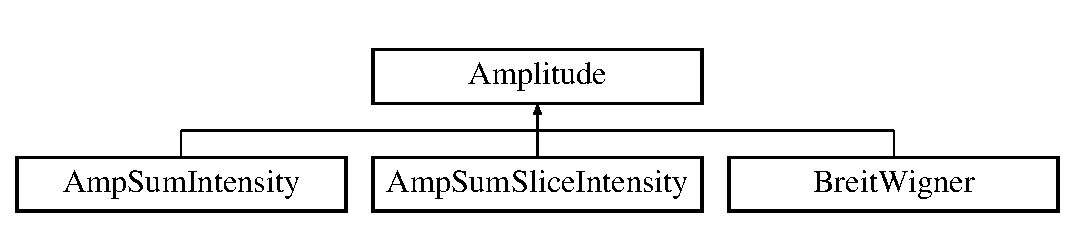
\includegraphics[height=2.000000cm]{class_amplitude}
\end{center}
\end{figure}
\subsection*{Public Member Functions}
\begin{DoxyCompactItemize}
\item 
\hypertarget{class_amplitude_ae0ce9e61d0e567682b4fd0ffe3c01c6c}{virtual const double {\bfseries integral} (\hyperlink{class_parameter_list}{Parameter\-List} \&par)=0}\label{class_amplitude_ae0ce9e61d0e567682b4fd0ffe3c01c6c}

\item 
\hypertarget{class_amplitude_a9c26aadd4b27d678849ce5551f463300}{virtual const double {\bfseries intensity} (std\-::vector$<$ double $>$ \&x, \hyperlink{class_parameter_list}{Parameter\-List} \&par)=0}\label{class_amplitude_a9c26aadd4b27d678849ce5551f463300}

\item 
\hypertarget{class_amplitude_ab5c5185c8d84243e21ac9f116b7d54e8}{virtual const bool {\bfseries fill\-Start\-Par\-Vec} (\hyperlink{class_parameter_list}{Parameter\-List} \&out\-Par)=0}\label{class_amplitude_ab5c5185c8d84243e21ac9f116b7d54e8}

\item 
\hypertarget{class_amplitude_aa1f00245b62ac125eb90cf3c34b4f7d7}{virtual void {\bfseries print\-Amps} ()=0}\label{class_amplitude_aa1f00245b62ac125eb90cf3c34b4f7d7}

\item 
\hypertarget{class_amplitude_aa0ce8c00facb8f134d4b0595c8b151a2}{virtual double {\bfseries get\-Max\-Val} ()=0}\label{class_amplitude_aa0ce8c00facb8f134d4b0595c8b151a2}

\end{DoxyCompactItemize}


\subsection{Detailed Description}
Physics Interface Base-\/\-Class. 

The documentation for this class was generated from the following file\-:\begin{DoxyCompactItemize}
\item 
Physics/\hyperlink{_amplitude_8hpp}{Amplitude.\-hpp}\end{DoxyCompactItemize}

\hypertarget{class_amplitude_setup}{\section{Amplitude\-Setup Class Reference}
\label{class_amplitude_setup}\index{Amplitude\-Setup@{Amplitude\-Setup}}
}


{\ttfamily \#include $<$Amplitude\-Setup.\-hpp$>$}

\subsection*{Public Member Functions}
\begin{DoxyCompactItemize}
\item 
\hypertarget{class_amplitude_setup_a7b0216893bfed41c13d975aa683d6012}{{\bfseries Amplitude\-Setup} (const std\-::string \&filename)}\label{class_amplitude_setup_a7b0216893bfed41c13d975aa683d6012}

\item 
\hypertarget{class_amplitude_setup_a9e415d3cca43cd3e8f42fcd29e3fda3c}{{\bfseries Amplitude\-Setup} (const \hyperlink{class_amplitude_setup}{Amplitude\-Setup} \&other)}\label{class_amplitude_setup_a9e415d3cca43cd3e8f42fcd29e3fda3c}

\item 
\hypertarget{class_amplitude_setup_a93e574c5c827a2a74e90b12302e658a3}{void {\bfseries load} (const std\-::string \&filename)}\label{class_amplitude_setup_a93e574c5c827a2a74e90b12302e658a3}

\item 
\hypertarget{class_amplitude_setup_a337a729509cc9af427c4b7afa7bbb72d}{void {\bfseries save} (const std\-::string \&filename)}\label{class_amplitude_setup_a337a729509cc9af427c4b7afa7bbb72d}

\item 
\hypertarget{class_amplitude_setup_a28cb86bfdfd0ddadbbad64dfec88a16e}{const std\-::string \& {\bfseries get\-File\-Name} () const }\label{class_amplitude_setup_a28cb86bfdfd0ddadbbad64dfec88a16e}

\item 
\hypertarget{class_amplitude_setup_a75045bb7b79b7b315069e6f0267873a4}{std\-::vector$<$ \hyperlink{struct_resonance}{Resonance} $>$ \& {\bfseries get\-Resonances} ()}\label{class_amplitude_setup_a75045bb7b79b7b315069e6f0267873a4}

\end{DoxyCompactItemize}


\subsection{Detailed Description}
This class is used to load an \hyperlink{class_amplitude}{Amplitude} configuration provided in an X\-M\-L file. As a Helper the struct \hyperlink{struct_resonance}{Resonance} is also provided, of which this class stores a vector. 

The documentation for this class was generated from the following file\-:\begin{DoxyCompactItemize}
\item 
Physics/\-Amplitude\-Sum/\hyperlink{_amplitude_setup_8hpp}{Amplitude\-Setup.\-hpp}\end{DoxyCompactItemize}

\hypertarget{class_amp_rel_breit_wigner_res}{\section{Amp\-Rel\-Breit\-Wigner\-Res Class Reference}
\label{class_amp_rel_breit_wigner_res}\index{Amp\-Rel\-Breit\-Wigner\-Res@{Amp\-Rel\-Breit\-Wigner\-Res}}
}
Inheritance diagram for Amp\-Rel\-Breit\-Wigner\-Res\-:\begin{figure}[H]
\begin{center}
\leavevmode
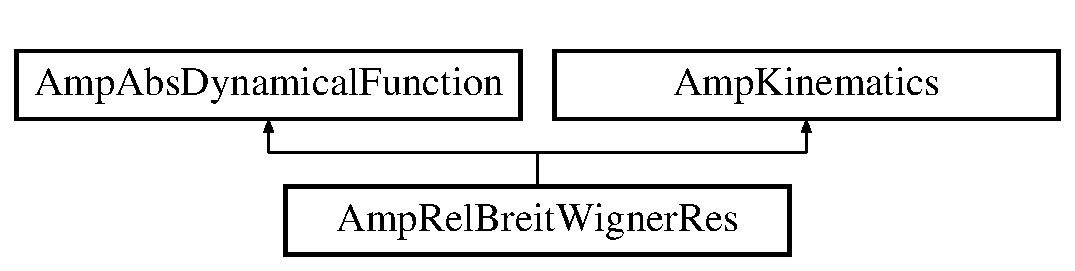
\includegraphics[height=2.000000cm]{class_amp_rel_breit_wigner_res}
\end{center}
\end{figure}
\subsection*{Public Member Functions}
\begin{DoxyCompactItemize}
\item 
\hypertarget{class_amp_rel_breit_wigner_res_af71461e1dcfea083ae7a754bbe4c8b9f}{{\bfseries Amp\-Rel\-Breit\-Wigner\-Res} (const char $\ast$name, \hyperlink{class_double_parameter}{Double\-Parameter} \&\-\_\-res\-Mass, \hyperlink{class_double_parameter}{Double\-Parameter} \&\-\_\-res\-Width, double \&\-\_\-radius, int \-\_\-subsys, int res\-Spin, int m, int n)}\label{class_amp_rel_breit_wigner_res_af71461e1dcfea083ae7a754bbe4c8b9f}

\item 
\hypertarget{class_amp_rel_breit_wigner_res_a610a71a571473034617d1a45147525ca}{{\bfseries Amp\-Rel\-Breit\-Wigner\-Res} (const \hyperlink{class_amp_rel_breit_wigner_res}{Amp\-Rel\-Breit\-Wigner\-Res} \&, const char $\ast$)}\label{class_amp_rel_breit_wigner_res_a610a71a571473034617d1a45147525ca}

\item 
\hypertarget{class_amp_rel_breit_wigner_res_a4ea1461b07cdd47c28f023c895d8078f}{{\bfseries Amp\-Rel\-Breit\-Wigner\-Res} (const \hyperlink{class_amp_rel_breit_wigner_res}{Amp\-Rel\-Breit\-Wigner\-Res} \&)}\label{class_amp_rel_breit_wigner_res_a4ea1461b07cdd47c28f023c895d8078f}

\item 
\hypertarget{class_amp_rel_breit_wigner_res_a157a0fe4973d10bfb002eb065ff341bd}{virtual void {\bfseries initialise} ()}\label{class_amp_rel_breit_wigner_res_a157a0fe4973d10bfb002eb065ff341bd}

\item 
\hypertarget{class_amp_rel_breit_wigner_res_a92e4278d123988fdda4a7a79eb95e7d9}{virtual std\-::complex$<$ double $>$ {\bfseries evaluate} () const }\label{class_amp_rel_breit_wigner_res_a92e4278d123988fdda4a7a79eb95e7d9}

\item 
\hypertarget{class_amp_rel_breit_wigner_res_a0a1b827174d03cb8653e917103287fea}{void {\bfseries set\-Decay\-Masses} (double, double, double, double)}\label{class_amp_rel_breit_wigner_res_a0a1b827174d03cb8653e917103287fea}

\item 
\hypertarget{class_amp_rel_breit_wigner_res_a85bd139a8892bf7d3e80b9c54d93adf8}{double {\bfseries integral} () const }\label{class_amp_rel_breit_wigner_res_a85bd139a8892bf7d3e80b9c54d93adf8}

\item 
\hypertarget{class_amp_rel_breit_wigner_res_afef3034eb12233fc25dc2227bf29fc01}{double {\bfseries get\-Spin} ()}\label{class_amp_rel_breit_wigner_res_afef3034eb12233fc25dc2227bf29fc01}

\item 
\hypertarget{class_amp_rel_breit_wigner_res_aba77f30f583c0e70ebbc8967b674dbf8}{virtual bool {\bfseries is\-Sub\-Sys} (const unsigned int sub\-Sys) const }\label{class_amp_rel_breit_wigner_res_aba77f30f583c0e70ebbc8967b674dbf8}

\end{DoxyCompactItemize}
\subsection*{Protected Attributes}
\begin{DoxyCompactItemize}
\item 
\hypertarget{class_amp_rel_breit_wigner_res_a05d7b775ee20505e42b699870ca99441}{\hyperlink{class_double_parameter}{Double\-Parameter} {\bfseries \-\_\-res\-Width}}\label{class_amp_rel_breit_wigner_res_a05d7b775ee20505e42b699870ca99441}

\item 
\hypertarget{class_amp_rel_breit_wigner_res_a421833c73971ecd0c5a9d478a0798c13}{\hyperlink{class_amp_wigner}{Amp\-Wigner} {\bfseries \-\_\-wigner\-D}}\label{class_amp_rel_breit_wigner_res_a421833c73971ecd0c5a9d478a0798c13}

\end{DoxyCompactItemize}
\subsection*{Additional Inherited Members}


The documentation for this class was generated from the following files\-:\begin{DoxyCompactItemize}
\item 
Physics/\-Amplitude\-Sum/Amp\-Rel\-Breit\-Wigner\-Res.\-hpp\item 
Physics/\-Amplitude\-Sum/Amp\-Rel\-Breit\-Wigner\-Res.\-cpp\end{DoxyCompactItemize}

\hypertarget{class_amp_sum_intensity}{\section{Amp\-Sum\-Intensity Class Reference}
\label{class_amp_sum_intensity}\index{Amp\-Sum\-Intensity@{Amp\-Sum\-Intensity}}
}
Inheritance diagram for Amp\-Sum\-Intensity\-:\begin{figure}[H]
\begin{center}
\leavevmode
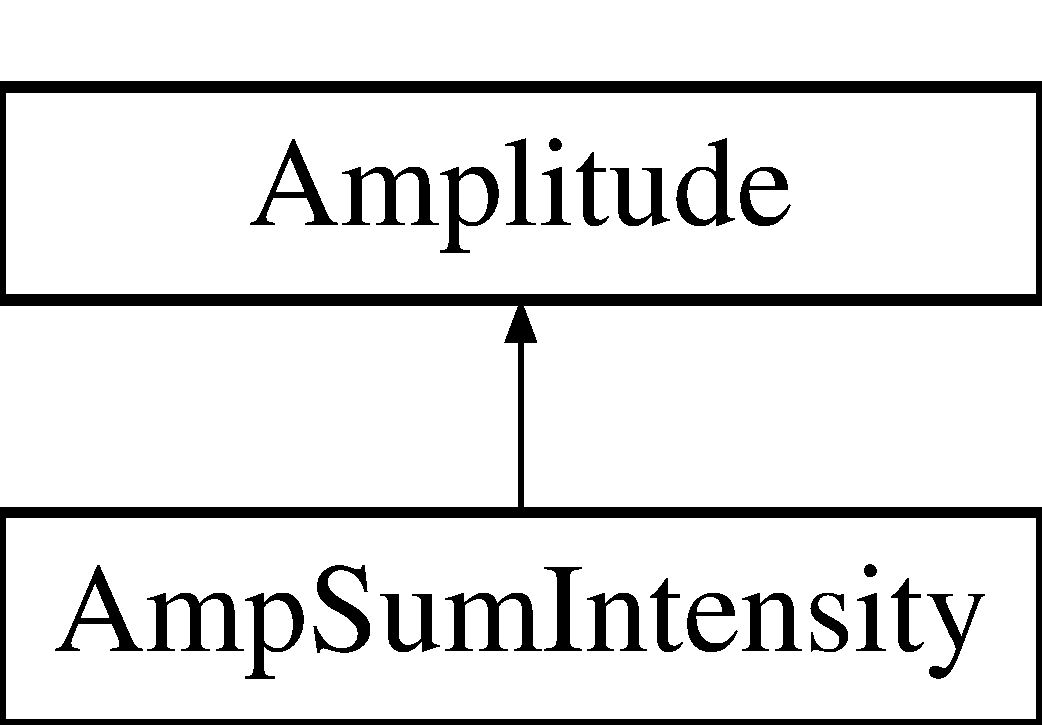
\includegraphics[height=2.000000cm]{class_amp_sum_intensity}
\end{center}
\end{figure}
\subsection*{Public Member Functions}
\begin{DoxyCompactItemize}
\item 
\hypertarget{class_amp_sum_intensity_abf5de602d6f8960805a105036754cb48}{\hyperlink{class_amp_sum_intensity_abf5de602d6f8960805a105036754cb48}{Amp\-Sum\-Intensity} (const double in\-M, const double in\-Br, const double in1, const double in2, const double in3, \hyperlink{class_amplitude_setup}{Amplitude\-Setup} ini)}\label{class_amp_sum_intensity_abf5de602d6f8960805a105036754cb48}

\begin{DoxyCompactList}\small\item\em Default Constructor (0x0) \end{DoxyCompactList}\item 
\hypertarget{class_amp_sum_intensity_ac5e45d36c35d8be011d37661d4a3a290}{\hyperlink{class_amp_sum_intensity_ac5e45d36c35d8be011d37661d4a3a290}{Amp\-Sum\-Intensity} (\hyperlink{class_d_p_kinematics}{D\-P\-Kinematics} kin, \hyperlink{class_amplitude_setup}{Amplitude\-Setup} ini)}\label{class_amp_sum_intensity_ac5e45d36c35d8be011d37661d4a3a290}

\begin{DoxyCompactList}\small\item\em Default Constructor (0x0) \end{DoxyCompactList}\item 
\hypertarget{class_amp_sum_intensity_a1214ad0183f6269bc0f53bb75eaa393a}{double {\bfseries get\-Max\-Val} ()}\label{class_amp_sum_intensity_a1214ad0183f6269bc0f53bb75eaa393a}

\item 
\hypertarget{class_amp_sum_intensity_aa864d46a78d52843d7fb4774244103a0}{virtual const double {\bfseries integral} (\hyperlink{class_parameter_list}{Parameter\-List} \&par)}\label{class_amp_sum_intensity_aa864d46a78d52843d7fb4774244103a0}

\item 
\hypertarget{class_amp_sum_intensity_a58c7d7fcc155adaa4bb93b28a7c21228}{virtual const double {\bfseries intensity} (std\-::vector$<$ double $>$ \&x, \hyperlink{class_parameter_list}{Parameter\-List} \&par)}\label{class_amp_sum_intensity_a58c7d7fcc155adaa4bb93b28a7c21228}

\item 
\hypertarget{class_amp_sum_intensity_a08fe49ab53719fb9a3ea687c4cf18ed0}{virtual const double {\bfseries intensity} (\hyperlink{class_parameter_list}{Parameter\-List} \&par)}\label{class_amp_sum_intensity_a08fe49ab53719fb9a3ea687c4cf18ed0}

\item 
\hypertarget{class_amp_sum_intensity_a5836b640fcd3270cc2ab5b730ae50b35}{virtual const bool {\bfseries fill\-Start\-Par\-Vec} (\hyperlink{class_parameter_list}{Parameter\-List} \&out\-Par)}\label{class_amp_sum_intensity_a5836b640fcd3270cc2ab5b730ae50b35}

\item 
\hypertarget{class_amp_sum_intensity_ae84ea31434dacf7cfaeed06c3f3fb414}{virtual void {\bfseries print\-Amps} ()}\label{class_amp_sum_intensity_ae84ea31434dacf7cfaeed06c3f3fb414}

\end{DoxyCompactItemize}
\subsection*{Protected Member Functions}
\begin{DoxyCompactItemize}
\item 
\hypertarget{class_amp_sum_intensity_a5c9786f704fc4f686705afb44fd47b45}{void {\bfseries init} ()}\label{class_amp_sum_intensity_a5c9786f704fc4f686705afb44fd47b45}

\end{DoxyCompactItemize}
\subsection*{Protected Attributes}
\begin{DoxyCompactItemize}
\item 
\hypertarget{class_amp_sum_intensity_a24e09e42bab4e0e3834211b5ab601ccd}{const \hyperlink{class_d_p_kinematics}{D\-P\-Kinematics} {\bfseries \-\_\-kin}}\label{class_amp_sum_intensity_a24e09e42bab4e0e3834211b5ab601ccd}

\item 
\hypertarget{class_amp_sum_intensity_a914c9d9f2f9f84dea2b33f116877e8f0}{\hyperlink{class_amp_sum_of_amplitudes}{Amp\-Sum\-Of\-Amplitudes} {\bfseries tot\-Amp}}\label{class_amp_sum_intensity_a914c9d9f2f9f84dea2b33f116877e8f0}

\item 
\hypertarget{class_amp_sum_intensity_a4b0409bf525e1f5b05f66180616f6d98}{\hyperlink{class_amplitude_setup}{Amplitude\-Setup} {\bfseries amp\-Setup}}\label{class_amp_sum_intensity_a4b0409bf525e1f5b05f66180616f6d98}

\item 
\hypertarget{class_amp_sum_intensity_a1dfcdd39ab646afcd747e46bab2249de}{double {\bfseries max\-Val}}\label{class_amp_sum_intensity_a1dfcdd39ab646afcd747e46bab2249de}

\item 
\hypertarget{class_amp_sum_intensity_a0e64c487233249ebb18edb279d200c03}{std\-::vector$<$ std\-::string $>$ {\bfseries namer}}\label{class_amp_sum_intensity_a0e64c487233249ebb18edb279d200c03}

\item 
\hypertarget{class_amp_sum_intensity_ac797ee706755fdc2ab5a3aa5cabbdb6f}{std\-::vector$<$ std\-::shared\-\_\-ptr\\*
$<$ \hyperlink{class_double_parameter}{Double\-Parameter} $>$ $>$ {\bfseries mr}}\label{class_amp_sum_intensity_ac797ee706755fdc2ab5a3aa5cabbdb6f}

\item 
\hypertarget{class_amp_sum_intensity_a4f66933d642894fe56a4a894f7e23a8e}{std\-::vector$<$ std\-::shared\-\_\-ptr\\*
$<$ \hyperlink{class_double_parameter}{Double\-Parameter} $>$ $>$ {\bfseries gr}}\label{class_amp_sum_intensity_a4f66933d642894fe56a4a894f7e23a8e}

\item 
\hypertarget{class_amp_sum_intensity_ad69912e6cd6789e48513083121da3120}{std\-::vector$<$ std\-::shared\-\_\-ptr\\*
$<$ \hyperlink{class_double_parameter}{Double\-Parameter} $>$ $>$ {\bfseries rr}}\label{class_amp_sum_intensity_ad69912e6cd6789e48513083121da3120}

\item 
\hypertarget{class_amp_sum_intensity_a0b3a45826506e6bcc07cfd4022a06478}{std\-::vector$<$ std\-::shared\-\_\-ptr\\*
$<$ \hyperlink{class_double_parameter}{Double\-Parameter} $>$ $>$ {\bfseries phir}}\label{class_amp_sum_intensity_a0b3a45826506e6bcc07cfd4022a06478}

\item 
\hypertarget{class_amp_sum_intensity_a0479f97ad59b4db627ac07456292f7b2}{std\-::vector$<$ std\-::shared\-\_\-ptr\\*
$<$ \hyperlink{class_double_parameter}{Double\-Parameter} $>$ $>$ {\bfseries qr}}\label{class_amp_sum_intensity_a0479f97ad59b4db627ac07456292f7b2}

\item 
\hypertarget{class_amp_sum_intensity_abd951e9bf7bd961432f5dcee5a2f7f33}{std\-::vector$<$ std\-::shared\-\_\-ptr\\*
$<$ \hyperlink{class_integer_parameter}{Integer\-Parameter} $>$ $>$ {\bfseries aj}}\label{class_amp_sum_intensity_abd951e9bf7bd961432f5dcee5a2f7f33}

\item 
\hypertarget{class_amp_sum_intensity_ad555e987005fe461da3265e689968e14}{std\-::vector$<$ std\-::shared\-\_\-ptr\\*
$<$ \hyperlink{class_integer_parameter}{Integer\-Parameter} $>$ $>$ {\bfseries am}}\label{class_amp_sum_intensity_ad555e987005fe461da3265e689968e14}

\item 
\hypertarget{class_amp_sum_intensity_a37869917dae55d554a3ae94c5ad70119}{std\-::vector$<$ std\-::shared\-\_\-ptr\\*
$<$ \hyperlink{class_integer_parameter}{Integer\-Parameter} $>$ $>$ {\bfseries an}}\label{class_amp_sum_intensity_a37869917dae55d554a3ae94c5ad70119}

\item 
\hypertarget{class_amp_sum_intensity_a3e132b7be0aa8170795f423e61c1aba7}{std\-::vector$<$ std\-::shared\-\_\-ptr\\*
$<$ \hyperlink{class_double_parameter}{Double\-Parameter} $>$ $>$ {\bfseries par1}}\label{class_amp_sum_intensity_a3e132b7be0aa8170795f423e61c1aba7}

\item 
\hypertarget{class_amp_sum_intensity_a9a8fcfd7539e78e97c15a2e4a09262e9}{std\-::vector$<$ std\-::shared\-\_\-ptr\\*
$<$ \hyperlink{class_double_parameter}{Double\-Parameter} $>$ $>$ {\bfseries par2}}\label{class_amp_sum_intensity_a9a8fcfd7539e78e97c15a2e4a09262e9}

\item 
\hypertarget{class_amp_sum_intensity_a057994051c08ae3bd7f8aa97213f3bd0}{std\-::vector$<$ std\-::shared\-\_\-ptr\\*
$<$ \hyperlink{class_amp_wigner}{Amp\-Wigner} $>$ $>$ {\bfseries angd}}\label{class_amp_sum_intensity_a057994051c08ae3bd7f8aa97213f3bd0}

\item 
\hypertarget{class_amp_sum_intensity_a08af6659c398af25cb3b070a4f19e961}{unsigned int {\bfseries n\-Amps}}\label{class_amp_sum_intensity_a08af6659c398af25cb3b070a4f19e961}

\end{DoxyCompactItemize}


The documentation for this class was generated from the following files\-:\begin{DoxyCompactItemize}
\item 
Physics/\-Amplitude\-Sum/Amp\-Sum\-Intensity.\-hpp\item 
Physics/\-Amplitude\-Sum/Amp\-Sum\-Intensity.\-cpp\end{DoxyCompactItemize}

\hypertarget{class_amp_sum_of_amplitudes}{\section{Amp\-Sum\-Of\-Amplitudes Class Reference}
\label{class_amp_sum_of_amplitudes}\index{Amp\-Sum\-Of\-Amplitudes@{Amp\-Sum\-Of\-Amplitudes}}
}
\subsection*{Public Member Functions}
\begin{DoxyCompactItemize}
\item 
\hypertarget{class_amp_sum_of_amplitudes_a978ca211858e8caa2d76817493dd4d65}{{\bfseries Amp\-Sum\-Of\-Amplitudes} (const char $\ast$name)}\label{class_amp_sum_of_amplitudes_a978ca211858e8caa2d76817493dd4d65}

\item 
\hypertarget{class_amp_sum_of_amplitudes_a0ae9ae3c2d26ba0e2f0dea9ed3848ad3}{{\bfseries Amp\-Sum\-Of\-Amplitudes} (const \hyperlink{class_amp_sum_of_amplitudes}{Amp\-Sum\-Of\-Amplitudes} \&other, const char $\ast$name=0)}\label{class_amp_sum_of_amplitudes_a0ae9ae3c2d26ba0e2f0dea9ed3848ad3}

\item 
\hypertarget{class_amp_sum_of_amplitudes_abd10da2566cce5a11e57812fdf678554}{void {\bfseries add\-B\-W} (std\-::shared\-\_\-ptr$<$ \hyperlink{class_amp_abs_dynamical_function}{Amp\-Abs\-Dynamical\-Function} $>$, std\-::shared\-\_\-ptr$<$ \hyperlink{class_double_parameter}{Double\-Parameter} $>$, std\-::shared\-\_\-ptr$<$ \hyperlink{class_double_parameter}{Double\-Parameter} $>$)}\label{class_amp_sum_of_amplitudes_abd10da2566cce5a11e57812fdf678554}

\item 
\hypertarget{class_amp_sum_of_amplitudes_a1500e62dc5c3fe7d4423238705e0b19f}{void {\bfseries add\-B\-W} (std\-::shared\-\_\-ptr$<$ \hyperlink{class_amp_abs_dynamical_function}{Amp\-Abs\-Dynamical\-Function} $>$, std\-::shared\-\_\-ptr$<$ \hyperlink{class_double_parameter}{Double\-Parameter} $>$, std\-::shared\-\_\-ptr$<$ \hyperlink{class_double_parameter}{Double\-Parameter} $>$, std\-::shared\-\_\-ptr$<$ \hyperlink{class_amp_wigner}{Amp\-Wigner} $>$)}\label{class_amp_sum_of_amplitudes_a1500e62dc5c3fe7d4423238705e0b19f}

\item 
\hypertarget{class_amp_sum_of_amplitudes_ac60d21d59ef7427c1dcdf300e6f59f0b}{double {\bfseries evaluate\-Slice} (std\-::complex$<$ double $>$ $\ast$, unsigned int, unsigned int) const }\label{class_amp_sum_of_amplitudes_ac60d21d59ef7427c1dcdf300e6f59f0b}

\item 
\hypertarget{class_amp_sum_of_amplitudes_abc905466c8533801103d3ae5e69d4c34}{double {\bfseries evaluate} () const }\label{class_amp_sum_of_amplitudes_abc905466c8533801103d3ae5e69d4c34}

\end{DoxyCompactItemize}
\subsection*{Protected Attributes}
\begin{DoxyCompactItemize}
\item 
\hypertarget{class_amp_sum_of_amplitudes_abce84ba0526d987145e73b66854c23be}{std\-::vector$<$ std\-::shared\-\_\-ptr\\*
$<$ \hyperlink{class_amp_abs_dynamical_function}{Amp\-Abs\-Dynamical\-Function} $>$ $>$ {\bfseries \-\_\-pdf\-List}}\label{class_amp_sum_of_amplitudes_abce84ba0526d987145e73b66854c23be}

\item 
\hypertarget{class_amp_sum_of_amplitudes_aeacd8c6289bb13006a6bb5ebb87a3649}{std\-::vector$<$ std\-::shared\-\_\-ptr\\*
$<$ \hyperlink{class_double_parameter}{Double\-Parameter} $>$ $>$ {\bfseries \-\_\-int\-List}}\label{class_amp_sum_of_amplitudes_aeacd8c6289bb13006a6bb5ebb87a3649}

\item 
\hypertarget{class_amp_sum_of_amplitudes_a4fb6f6f7024be7bec8ba2b3707c9b1cb}{std\-::vector$<$ std\-::shared\-\_\-ptr\\*
$<$ \hyperlink{class_double_parameter}{Double\-Parameter} $>$ $>$ {\bfseries \-\_\-phase\-List}}\label{class_amp_sum_of_amplitudes_a4fb6f6f7024be7bec8ba2b3707c9b1cb}

\item 
\hypertarget{class_amp_sum_of_amplitudes_a8af3b5a2e4a5bcf2d7da97239445d1c5}{std\-::vector$<$ std\-::shared\-\_\-ptr\\*
$<$ \hyperlink{class_amp_wigner}{Amp\-Wigner} $>$ $>$ {\bfseries \-\_\-ang\-List}}\label{class_amp_sum_of_amplitudes_a8af3b5a2e4a5bcf2d7da97239445d1c5}

\item 
\hypertarget{class_amp_sum_of_amplitudes_aa982dc609e1e35765ce6172cef895f90}{double {\bfseries max\-Val}}\label{class_amp_sum_of_amplitudes_aa982dc609e1e35765ce6172cef895f90}

\end{DoxyCompactItemize}


The documentation for this class was generated from the following files\-:\begin{DoxyCompactItemize}
\item 
Physics/\-Amplitude\-Sum/Amp\-Sum\-Of\-Amplitudes.\-hpp\item 
Physics/\-Amplitude\-Sum/Amp\-Sum\-Of\-Amplitudes.\-cpp\end{DoxyCompactItemize}

\hypertarget{class_amp_sum_slice_intensity}{\section{Amp\-Sum\-Slice\-Intensity Class Reference}
\label{class_amp_sum_slice_intensity}\index{Amp\-Sum\-Slice\-Intensity@{Amp\-Sum\-Slice\-Intensity}}
}
Inheritance diagram for Amp\-Sum\-Slice\-Intensity\-:\begin{figure}[H]
\begin{center}
\leavevmode
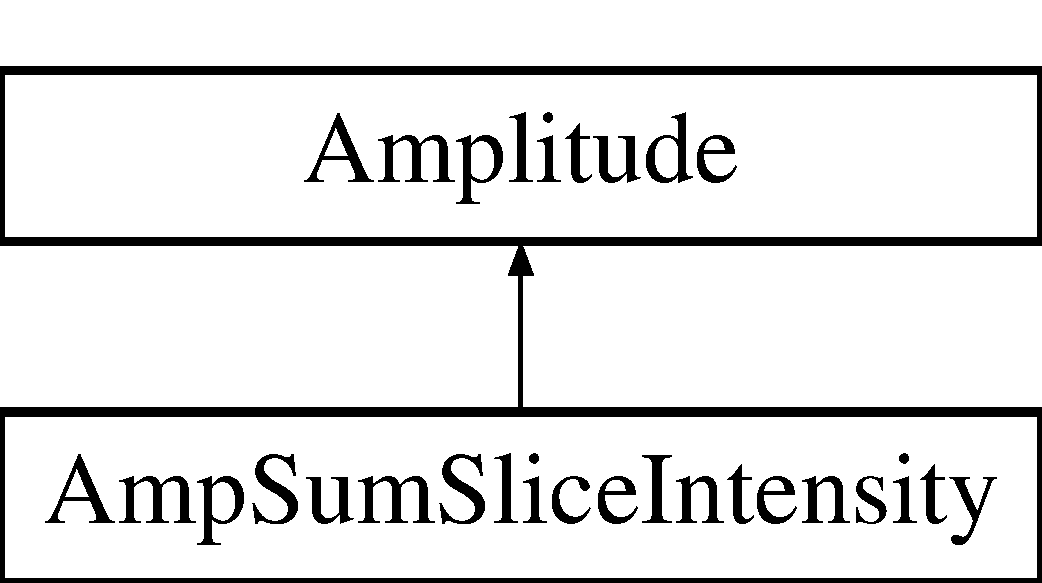
\includegraphics[height=2.000000cm]{class_amp_sum_slice_intensity}
\end{center}
\end{figure}
\subsection*{Public Member Functions}
\begin{DoxyCompactItemize}
\item 
\hypertarget{class_amp_sum_slice_intensity_a84184310702a57fe213ef21d341f5c4e}{\hyperlink{class_amp_sum_slice_intensity_a84184310702a57fe213ef21d341f5c4e}{Amp\-Sum\-Slice\-Intensity} (const double in\-M, const double in\-Br, const double in1, const double in2, const double in3, \hyperlink{class_amplitude_setup}{Amplitude\-Setup} ini)}\label{class_amp_sum_slice_intensity_a84184310702a57fe213ef21d341f5c4e}

\begin{DoxyCompactList}\small\item\em Default Constructor (0x0) \end{DoxyCompactList}\item 
\hypertarget{class_amp_sum_slice_intensity_aeef9bdb403caa91ca4bf8615627ca6fc}{virtual const double {\bfseries integral} (\hyperlink{class_parameter_list}{Parameter\-List} \&par)}\label{class_amp_sum_slice_intensity_aeef9bdb403caa91ca4bf8615627ca6fc}

\item 
\hypertarget{class_amp_sum_slice_intensity_a845d93e9216f2af4057715ce879d3989}{virtual const double {\bfseries intensity} (std\-::vector$<$ double $>$ \&x, \hyperlink{class_parameter_list}{Parameter\-List} \&par)}\label{class_amp_sum_slice_intensity_a845d93e9216f2af4057715ce879d3989}

\item 
\hypertarget{class_amp_sum_slice_intensity_ac9eda7d89099198806b0acd365acf884}{virtual const bool {\bfseries fill\-Start\-Par\-Vec} (\hyperlink{class_parameter_list}{Parameter\-List} \&out\-Par)}\label{class_amp_sum_slice_intensity_ac9eda7d89099198806b0acd365acf884}

\item 
virtual \hyperlink{class_amp_sum_slice_intensity_aec60ef699833a82fd1d3705c0d889a42}{$\sim$\-Amp\-Sum\-Slice\-Intensity} ()
\item 
\hypertarget{class_amp_sum_slice_intensity_a8badde30f0af858cf9bbbe74b3001813}{double {\bfseries get\-Max\-Val} ()}\label{class_amp_sum_slice_intensity_a8badde30f0af858cf9bbbe74b3001813}

\end{DoxyCompactItemize}
\subsection*{Protected Member Functions}
\begin{DoxyCompactItemize}
\item 
\hypertarget{class_amp_sum_slice_intensity_a4bbe6e0b6b52ad563a1ad88372269d70}{double {\bfseries lambda} (double x, double y, double z)}\label{class_amp_sum_slice_intensity_a4bbe6e0b6b52ad563a1ad88372269d70}

\item 
\hypertarget{class_amp_sum_slice_intensity_af1d052cb4d842fa0c138720bbca1e3c0}{double {\bfseries m13\-\_\-sq\-\_\-max\-\_\-constr} (double \&m23\-\_\-sq)}\label{class_amp_sum_slice_intensity_af1d052cb4d842fa0c138720bbca1e3c0}

\item 
\hypertarget{class_amp_sum_slice_intensity_ace69c74b9f40855821e2176953a8c0e7}{double {\bfseries m13\-\_\-sq\-\_\-min\-\_\-constr} (double \&m23\-\_\-sq)}\label{class_amp_sum_slice_intensity_ace69c74b9f40855821e2176953a8c0e7}

\item 
\hypertarget{class_amp_sum_slice_intensity_aa090b258891725259e61686abbf4ef8c}{double {\bfseries m23\-\_\-sq\-\_\-max\-\_\-constr} (double \&m13\-\_\-sq)}\label{class_amp_sum_slice_intensity_aa090b258891725259e61686abbf4ef8c}

\item 
\hypertarget{class_amp_sum_slice_intensity_ad8c7b32e6980dff167248aef0173796d}{double {\bfseries m23\-\_\-sq\-\_\-min\-\_\-constr} (double \&m13\-\_\-sq)}\label{class_amp_sum_slice_intensity_ad8c7b32e6980dff167248aef0173796d}

\item 
\hypertarget{class_amp_sum_slice_intensity_a65040ff02976a9822736d54376f00473}{double {\bfseries mb\-\_\-sq\-\_\-max\-\_\-constr} (double \&ma\-\_\-sq)}\label{class_amp_sum_slice_intensity_a65040ff02976a9822736d54376f00473}

\item 
\hypertarget{class_amp_sum_slice_intensity_a4ebb653e40a69fdc1da2a33d995b2d19}{double {\bfseries mb\-\_\-sq\-\_\-min\-\_\-constr} (double \&ma\-\_\-sq)}\label{class_amp_sum_slice_intensity_a4ebb653e40a69fdc1da2a33d995b2d19}

\item 
\hypertarget{class_amp_sum_slice_intensity_a143f11330f52d2073aaee9603ff8a574}{double {\bfseries ma\-\_\-sq\-\_\-max\-\_\-constr} (double \&mb\-\_\-sq)}\label{class_amp_sum_slice_intensity_a143f11330f52d2073aaee9603ff8a574}

\item 
\hypertarget{class_amp_sum_slice_intensity_aaa93035c162cfa0c02f06c27382d17d9}{double {\bfseries ma\-\_\-sq\-\_\-min\-\_\-constr} (double \&mb\-\_\-sq)}\label{class_amp_sum_slice_intensity_aaa93035c162cfa0c02f06c27382d17d9}

\end{DoxyCompactItemize}
\subsection*{Protected Attributes}
\begin{DoxyCompactItemize}
\item 
\hypertarget{class_amp_sum_slice_intensity_a8af6b8e147e36b1221eb8401a74a7f83}{const Double\-\_\-t {\bfseries M}}\label{class_amp_sum_slice_intensity_a8af6b8e147e36b1221eb8401a74a7f83}

\item 
\hypertarget{class_amp_sum_slice_intensity_ac630eae45343a64d19f70d266969a11a}{const Double\-\_\-t {\bfseries Br}}\label{class_amp_sum_slice_intensity_ac630eae45343a64d19f70d266969a11a}

\item 
\hypertarget{class_amp_sum_slice_intensity_ad906d5023aae5e0db37ccfd1c56cd0d5}{const Double\-\_\-t {\bfseries m1}}\label{class_amp_sum_slice_intensity_ad906d5023aae5e0db37ccfd1c56cd0d5}

\item 
\hypertarget{class_amp_sum_slice_intensity_abcf5a6d35ad7c2c77bebaa3998e0c26d}{const Double\-\_\-t {\bfseries m2}}\label{class_amp_sum_slice_intensity_abcf5a6d35ad7c2c77bebaa3998e0c26d}

\item 
\hypertarget{class_amp_sum_slice_intensity_a60f0cfc2cec833be55a6e3627295bcae}{const Double\-\_\-t {\bfseries m3}}\label{class_amp_sum_slice_intensity_a60f0cfc2cec833be55a6e3627295bcae}

\item 
\hypertarget{class_amp_sum_slice_intensity_a67a1198da438c77a3f4147162b47cd09}{const Double\-\_\-t {\bfseries P\-I}}\label{class_amp_sum_slice_intensity_a67a1198da438c77a3f4147162b47cd09}

\item 
\hypertarget{class_amp_sum_slice_intensity_ac70973fd4edf995940b9ba618366496c}{const Double\-\_\-t {\bfseries m23\-\_\-sq\-\_\-min}}\label{class_amp_sum_slice_intensity_ac70973fd4edf995940b9ba618366496c}

\item 
\hypertarget{class_amp_sum_slice_intensity_abab3af275f3fbe41b09eb78803a6689b}{const Double\-\_\-t {\bfseries m23\-\_\-sq\-\_\-max}}\label{class_amp_sum_slice_intensity_abab3af275f3fbe41b09eb78803a6689b}

\item 
\hypertarget{class_amp_sum_slice_intensity_a77684486f6f074b1629bd486816fd684}{const Double\-\_\-t {\bfseries m13\-\_\-sq\-\_\-min}}\label{class_amp_sum_slice_intensity_a77684486f6f074b1629bd486816fd684}

\item 
\hypertarget{class_amp_sum_slice_intensity_ad8efbec42aa2890e5096c4ddb877ec5e}{const Double\-\_\-t {\bfseries m13\-\_\-sq\-\_\-max}}\label{class_amp_sum_slice_intensity_ad8efbec42aa2890e5096c4ddb877ec5e}

\item 
\hypertarget{class_amp_sum_slice_intensity_aeda2c58590a0cd53c1f5a463849e24cf}{const Double\-\_\-t {\bfseries m12\-\_\-sq\-\_\-min}}\label{class_amp_sum_slice_intensity_aeda2c58590a0cd53c1f5a463849e24cf}

\item 
\hypertarget{class_amp_sum_slice_intensity_ad0415fe12520dfef1dfe5157f01b27a6}{const Double\-\_\-t {\bfseries m12\-\_\-sq\-\_\-max}}\label{class_amp_sum_slice_intensity_ad0415fe12520dfef1dfe5157f01b27a6}

\item 
\hypertarget{class_amp_sum_slice_intensity_a4b9ebd03284f324bba951f91d130ea7f}{const Double\-\_\-t {\bfseries m23\-\_\-min}}\label{class_amp_sum_slice_intensity_a4b9ebd03284f324bba951f91d130ea7f}

\item 
\hypertarget{class_amp_sum_slice_intensity_acaf58a9c19a5a2adaeb1fb260eb74768}{const Double\-\_\-t {\bfseries m23\-\_\-max}}\label{class_amp_sum_slice_intensity_acaf58a9c19a5a2adaeb1fb260eb74768}

\item 
\hypertarget{class_amp_sum_slice_intensity_a3ead9bb6021629db116189d8ec473670}{const Double\-\_\-t {\bfseries m13\-\_\-min}}\label{class_amp_sum_slice_intensity_a3ead9bb6021629db116189d8ec473670}

\item 
\hypertarget{class_amp_sum_slice_intensity_ac0d3f6aab1ba4c73b606158ad2b20e9e}{const Double\-\_\-t {\bfseries m13\-\_\-max}}\label{class_amp_sum_slice_intensity_ac0d3f6aab1ba4c73b606158ad2b20e9e}

\item 
\hypertarget{class_amp_sum_slice_intensity_a2d05a21757e608fdf4cad6ef1330076b}{const Double\-\_\-t {\bfseries m12\-\_\-min}}\label{class_amp_sum_slice_intensity_a2d05a21757e608fdf4cad6ef1330076b}

\item 
\hypertarget{class_amp_sum_slice_intensity_aa8e0d765154598908e3eefbaf5171810}{const Double\-\_\-t {\bfseries m12\-\_\-max}}\label{class_amp_sum_slice_intensity_aa8e0d765154598908e3eefbaf5171810}

\item 
\hypertarget{class_amp_sum_slice_intensity_ac32a8930e852443436947a41f0f6a7fa}{Roo\-Real\-Var {\bfseries ma}}\label{class_amp_sum_slice_intensity_ac32a8930e852443436947a41f0f6a7fa}

\item 
\hypertarget{class_amp_sum_slice_intensity_ac6f605234c3b88760cfe707ad8c60002}{Roo\-Real\-Var {\bfseries mb}}\label{class_amp_sum_slice_intensity_ac6f605234c3b88760cfe707ad8c60002}

\item 
\hypertarget{class_amp_sum_slice_intensity_aa67eb2fcc0109235caf11f16eba73f2f}{Roo\-Real\-Var {\bfseries mc}}\label{class_amp_sum_slice_intensity_aa67eb2fcc0109235caf11f16eba73f2f}

\item 
\hypertarget{class_amp_sum_slice_intensity_a610be27a33171131fa2c9f8651ba38fe}{\hyperlink{class_amp_sum_of_amplitudes}{Amp\-Sum\-Of\-Amplitudes} {\bfseries tot\-Amp}}\label{class_amp_sum_slice_intensity_a610be27a33171131fa2c9f8651ba38fe}

\item 
\hypertarget{class_amp_sum_slice_intensity_a8d61ddb87f8a6f5b1958659c32e8cee3}{std\-::vector$<$ std\-::shared\-\_\-ptr\\*
$<$ Roo\-Real\-Var $>$ $>$ {\bfseries mr}}\label{class_amp_sum_slice_intensity_a8d61ddb87f8a6f5b1958659c32e8cee3}

\item 
\hypertarget{class_amp_sum_slice_intensity_ac67dd97a2e4ceb2a51ccdea990d65561}{std\-::vector$<$ std\-::shared\-\_\-ptr\\*
$<$ Roo\-Real\-Var $>$ $>$ {\bfseries qr}}\label{class_amp_sum_slice_intensity_ac67dd97a2e4ceb2a51ccdea990d65561}

\item 
\hypertarget{class_amp_sum_slice_intensity_aeb8eefedfb2215bdd2d4672281e95ba7}{std\-::vector$<$ std\-::shared\-\_\-ptr\\*
$<$ Roo\-Real\-Var $>$ $>$ {\bfseries gr}}\label{class_amp_sum_slice_intensity_aeb8eefedfb2215bdd2d4672281e95ba7}

\item 
\hypertarget{class_amp_sum_slice_intensity_a36681de314dd1ba9c262456d0769bef9}{std\-::vector$<$ std\-::shared\-\_\-ptr\\*
$<$ Roo\-Real\-Var $>$ $>$ {\bfseries rr}}\label{class_amp_sum_slice_intensity_a36681de314dd1ba9c262456d0769bef9}

\item 
\hypertarget{class_amp_sum_slice_intensity_a07d3965e2c41e7cf26e2bae477bba85a}{std\-::vector$<$ std\-::shared\-\_\-ptr\\*
$<$ Roo\-Real\-Var $>$ $>$ {\bfseries phir}}\label{class_amp_sum_slice_intensity_a07d3965e2c41e7cf26e2bae477bba85a}

\item 
\hypertarget{class_amp_sum_slice_intensity_a4afc5345a81434510c5bdbb60451dd1c}{std\-::vector$<$ std\-::shared\-\_\-ptr\\*
$<$ Roo\-Real\-Var $>$ $>$ {\bfseries aj}}\label{class_amp_sum_slice_intensity_a4afc5345a81434510c5bdbb60451dd1c}

\item 
\hypertarget{class_amp_sum_slice_intensity_a95c80e5d1ac22ea9d64d1353c3ab2875}{std\-::vector$<$ std\-::shared\-\_\-ptr\\*
$<$ Roo\-Real\-Var $>$ $>$ {\bfseries am}}\label{class_amp_sum_slice_intensity_a95c80e5d1ac22ea9d64d1353c3ab2875}

\item 
\hypertarget{class_amp_sum_slice_intensity_ae42c56bdeff88da1a1dcc3242a0a6639}{std\-::vector$<$ std\-::shared\-\_\-ptr\\*
$<$ Roo\-Real\-Var $>$ $>$ {\bfseries an}}\label{class_amp_sum_slice_intensity_ae42c56bdeff88da1a1dcc3242a0a6639}

\item 
\hypertarget{class_amp_sum_slice_intensity_a403bf6e2359846fc975f83ada8a7a243}{std\-::vector$<$ std\-::shared\-\_\-ptr\\*
$<$ \hyperlink{class_amp_abs_dynamical_function}{Amp\-Abs\-Dynamical\-Function} $>$ $>$ {\bfseries rbw}}\label{class_amp_sum_slice_intensity_a403bf6e2359846fc975f83ada8a7a243}

\item 
\hypertarget{class_amp_sum_slice_intensity_aac5f25abe8d07d0a35fafc65c76acf4c}{std\-::vector$<$ std\-::shared\-\_\-ptr\\*
$<$ \hyperlink{class_amp_wigner}{Amp\-Wigner} $>$ $>$ {\bfseries angd}}\label{class_amp_sum_slice_intensity_aac5f25abe8d07d0a35fafc65c76acf4c}

\end{DoxyCompactItemize}


\subsection{Constructor \& Destructor Documentation}
\hypertarget{class_amp_sum_slice_intensity_aec60ef699833a82fd1d3705c0d889a42}{\index{Amp\-Sum\-Slice\-Intensity@{Amp\-Sum\-Slice\-Intensity}!$\sim$\-Amp\-Sum\-Slice\-Intensity@{$\sim$\-Amp\-Sum\-Slice\-Intensity}}
\index{$\sim$\-Amp\-Sum\-Slice\-Intensity@{$\sim$\-Amp\-Sum\-Slice\-Intensity}!AmpSumSliceIntensity@{Amp\-Sum\-Slice\-Intensity}}
\subsubsection[{$\sim$\-Amp\-Sum\-Slice\-Intensity}]{\setlength{\rightskip}{0pt plus 5cm}virtual Amp\-Sum\-Slice\-Intensity\-::$\sim$\-Amp\-Sum\-Slice\-Intensity (
\begin{DoxyParamCaption}
{}
\end{DoxyParamCaption}
)\hspace{0.3cm}{\ttfamily [inline]}, {\ttfamily [virtual]}}}\label{class_amp_sum_slice_intensity_aec60ef699833a82fd1d3705c0d889a42}
Destructor 

The documentation for this class was generated from the following file\-:\begin{DoxyCompactItemize}
\item 
Physics/\-Amplitude\-Sum/Amp\-Sum\-Slice\-Intensity.\-hpp\end{DoxyCompactItemize}

\hypertarget{class_amp_wigner}{\section{Amp\-Wigner Class Reference}
\label{class_amp_wigner}\index{Amp\-Wigner@{Amp\-Wigner}}
}
\subsection*{Public Member Functions}
\begin{DoxyCompactItemize}
\item 
\hypertarget{class_amp_wigner_a69f4e662e997ee0e69e9401ca46ad150}{{\bfseries Amp\-Wigner} (const char $\ast$name, unsigned int spin, unsigned int m, unsigned int n, unsigned int sub\-Sys)}\label{class_amp_wigner_a69f4e662e997ee0e69e9401ca46ad150}

\item 
\hypertarget{class_amp_wigner_a5407f785bfe94046cfbec4009943c628}{{\bfseries Amp\-Wigner} (const \hyperlink{class_amp_wigner}{Amp\-Wigner} \&, const char $\ast$)}\label{class_amp_wigner_a5407f785bfe94046cfbec4009943c628}

\item 
\hypertarget{class_amp_wigner_af46efef6ab12232a04237c92ac2bec89}{virtual bool {\bfseries has\-Dist} ()}\label{class_amp_wigner_af46efef6ab12232a04237c92ac2bec89}

\item 
\hypertarget{class_amp_wigner_aa396cb00c36a480f2656d401f2bc55a6}{virtual void {\bfseries initialise} ()}\label{class_amp_wigner_aa396cb00c36a480f2656d401f2bc55a6}

\item 
\hypertarget{class_amp_wigner_a5ba2441214fa10546f0f4724539c32ad}{virtual double {\bfseries evaluate} () const }\label{class_amp_wigner_a5ba2441214fa10546f0f4724539c32ad}

\item 
\hypertarget{class_amp_wigner_a7631b9cbe704f5ce46c9eaef059813ae}{void {\bfseries set\-Decay\-Masses} (double, double, double, double)}\label{class_amp_wigner_a7631b9cbe704f5ce46c9eaef059813ae}

\end{DoxyCompactItemize}
\subsection*{Protected Member Functions}
\begin{DoxyCompactItemize}
\item 
\hypertarget{class_amp_wigner_a22d44e5d6baea0ecb6d6d010556f0697}{double {\bfseries lambda} (double x, double y, double z) const }\label{class_amp_wigner_a22d44e5d6baea0ecb6d6d010556f0697}

\item 
\hypertarget{class_amp_wigner_a69e8834818de83c9e9c1fc4a19c52b80}{double {\bfseries s1max} (double, double, double, double, double) const }\label{class_amp_wigner_a69e8834818de83c9e9c1fc4a19c52b80}

\item 
\hypertarget{class_amp_wigner_abc3c3bb28f8d226a6b88f512b23b5bfd}{double {\bfseries s1min} (double, double, double, double, double) const }\label{class_amp_wigner_abc3c3bb28f8d226a6b88f512b23b5bfd}

\item 
\hypertarget{class_amp_wigner_a2fea03ef732b8068724803a352a1259a}{double {\bfseries s2max} (double, double, double, double, double) const }\label{class_amp_wigner_a2fea03ef732b8068724803a352a1259a}

\item 
\hypertarget{class_amp_wigner_a1a7dbcd27bb877b2b96416aa73e8a62d}{double {\bfseries s2min} (double, double, double, double, double) const }\label{class_amp_wigner_a1a7dbcd27bb877b2b96416aa73e8a62d}

\item 
\hypertarget{class_amp_wigner_a0ef62ba8228e9dee219e901511b3d30f}{double {\bfseries s3max} (double, double, double, double, double) const }\label{class_amp_wigner_a0ef62ba8228e9dee219e901511b3d30f}

\item 
\hypertarget{class_amp_wigner_ae1b5f51dad6538742e2ffa16f09ab559}{double {\bfseries s3min} (double, double, double, double, double) const }\label{class_amp_wigner_ae1b5f51dad6538742e2ffa16f09ab559}

\end{DoxyCompactItemize}
\subsection*{Protected Attributes}
\begin{DoxyCompactItemize}
\item 
\hypertarget{class_amp_wigner_ad9e35a3e41b2dc47c605cfda5e2785f6}{unsigned int {\bfseries \-\_\-in\-Spin}}\label{class_amp_wigner_ad9e35a3e41b2dc47c605cfda5e2785f6}

\item 
\hypertarget{class_amp_wigner_a6d0d70fbb59c071ac5ce1fef35eda1bc}{unsigned int {\bfseries \-\_\-out\-Spin1}}\label{class_amp_wigner_a6d0d70fbb59c071ac5ce1fef35eda1bc}

\item 
\hypertarget{class_amp_wigner_a9742040a6ce6a486b69d3590120050b1}{unsigned int {\bfseries \-\_\-out\-Spin2}}\label{class_amp_wigner_a9742040a6ce6a486b69d3590120050b1}

\item 
\hypertarget{class_amp_wigner_a863cebcb9a5ce10f5c2633f5307f1ed7}{unsigned int {\bfseries \-\_\-sub\-Sys}}\label{class_amp_wigner_a863cebcb9a5ce10f5c2633f5307f1ed7}

\item 
\hypertarget{class_amp_wigner_a32e856e58b4f803be41b29fd02a83a4d}{double {\bfseries \-\_\-\-M}}\label{class_amp_wigner_a32e856e58b4f803be41b29fd02a83a4d}

\item 
\hypertarget{class_amp_wigner_aa16c14c601d903f986408382c4f85a46}{double {\bfseries \-\_\-m1}}\label{class_amp_wigner_aa16c14c601d903f986408382c4f85a46}

\item 
\hypertarget{class_amp_wigner_a5216b522b1c493db5b1c56112945ff8f}{double {\bfseries \-\_\-m2}}\label{class_amp_wigner_a5216b522b1c493db5b1c56112945ff8f}

\item 
\hypertarget{class_amp_wigner_a9079195d22ad26b22bd309bdc3af7581}{double {\bfseries \-\_\-m3}}\label{class_amp_wigner_a9079195d22ad26b22bd309bdc3af7581}

\item 
\hypertarget{class_amp_wigner_adc9a253f9efd45d6781793f89154bc08}{bool {\bfseries to\-Evaluate}}\label{class_amp_wigner_adc9a253f9efd45d6781793f89154bc08}

\end{DoxyCompactItemize}


The documentation for this class was generated from the following files\-:\begin{DoxyCompactItemize}
\item 
Physics/\-Amplitude\-Sum/Amp\-Wigner.\-hpp\item 
Physics/\-Amplitude\-Sum/Amp\-Wigner.\-cpp\end{DoxyCompactItemize}

\hypertarget{class_ascii_reader}{\section{Ascii\-Reader Class Reference}
\label{class_ascii_reader}\index{Ascii\-Reader@{Ascii\-Reader}}
}
Inheritance diagram for Ascii\-Reader\-:\begin{figure}[H]
\begin{center}
\leavevmode
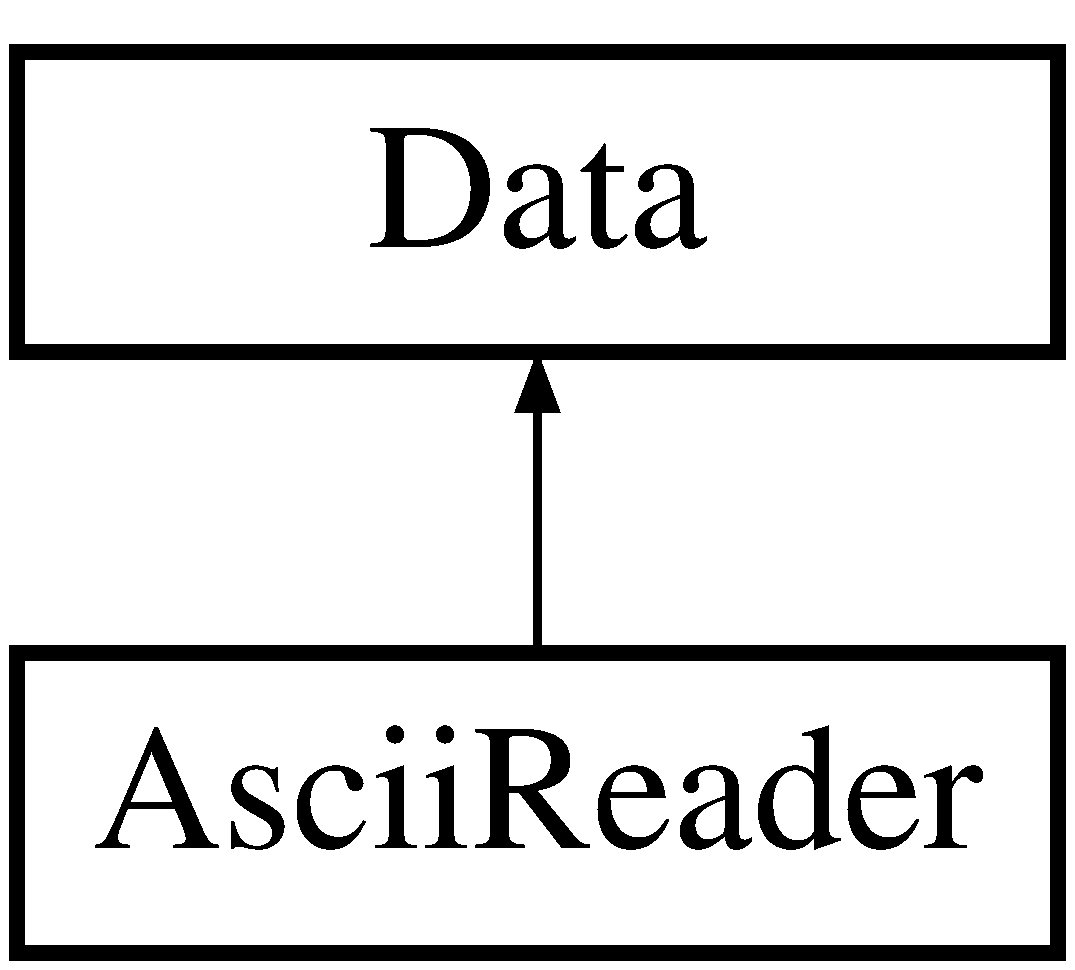
\includegraphics[height=2.000000cm]{class_ascii_reader}
\end{center}
\end{figure}
\subsection*{Public Member Functions}
\begin{DoxyCompactItemize}
\item 
\hypertarget{class_ascii_reader_a7e4d19ef330f588df7135343a1757ed2}{\hyperlink{class_ascii_reader_a7e4d19ef330f588df7135343a1757ed2}{Ascii\-Reader} (const std\-::string in\-Config\-File, const int particles)}\label{class_ascii_reader_a7e4d19ef330f588df7135343a1757ed2}

\begin{DoxyCompactList}\small\item\em Default Constructor (0x0) \end{DoxyCompactList}\item 
\hypertarget{class_ascii_reader_a908d6716adcb6dac4b018f6ebb2639f3}{virtual const \hyperlink{class_event}{Event} \& {\bfseries get\-Event} (const int)}\label{class_ascii_reader_a908d6716adcb6dac4b018f6ebb2639f3}

\item 
\hypertarget{class_ascii_reader_a6466d1cf0c68cab718278d065511577d}{virtual const int {\bfseries get\-Bin} (const int, double \&, double \&)}\label{class_ascii_reader_a6466d1cf0c68cab718278d065511577d}

\item 
\hypertarget{class_ascii_reader_add4df8989c883fc35d05cc95b8df0941}{virtual const unsigned int {\bfseries get\-N\-Events} () const }\label{class_ascii_reader_add4df8989c883fc35d05cc95b8df0941}

\item 
\hypertarget{class_ascii_reader_a4205de0cc54423de3f78654d059b07bc}{virtual const unsigned int {\bfseries get\-N\-Bins} () const }\label{class_ascii_reader_a4205de0cc54423de3f78654d059b07bc}

\item 
virtual \hyperlink{class_ascii_reader_a5b248943b9a4cb931ec58a00c31168d8}{$\sim$\-Ascii\-Reader} ()
\end{DoxyCompactItemize}


\subsection{Constructor \& Destructor Documentation}
\hypertarget{class_ascii_reader_a5b248943b9a4cb931ec58a00c31168d8}{\index{Ascii\-Reader@{Ascii\-Reader}!$\sim$\-Ascii\-Reader@{$\sim$\-Ascii\-Reader}}
\index{$\sim$\-Ascii\-Reader@{$\sim$\-Ascii\-Reader}!AsciiReader@{Ascii\-Reader}}
\subsubsection[{$\sim$\-Ascii\-Reader}]{\setlength{\rightskip}{0pt plus 5cm}Ascii\-Reader\-::$\sim$\-Ascii\-Reader (
\begin{DoxyParamCaption}
{}
\end{DoxyParamCaption}
)\hspace{0.3cm}{\ttfamily [virtual]}}}\label{class_ascii_reader_a5b248943b9a4cb931ec58a00c31168d8}
Destructor 

The documentation for this class was generated from the following files\-:\begin{DoxyCompactItemize}
\item 
Data\-Reader/\-Ascii\-Reader/Ascii\-Reader.\-h\item 
Data\-Reader/\-Ascii\-Reader/Ascii\-Reader.\-cpp\end{DoxyCompactItemize}

\hypertarget{class_bad_config}{\section{Bad\-Config Class Reference}
\label{class_bad_config}\index{Bad\-Config@{Bad\-Config}}
}


Config is not complete.  




{\ttfamily \#include $<$Exceptions.\-hpp$>$}

Inheritance diagram for Bad\-Config\-:\begin{figure}[H]
\begin{center}
\leavevmode
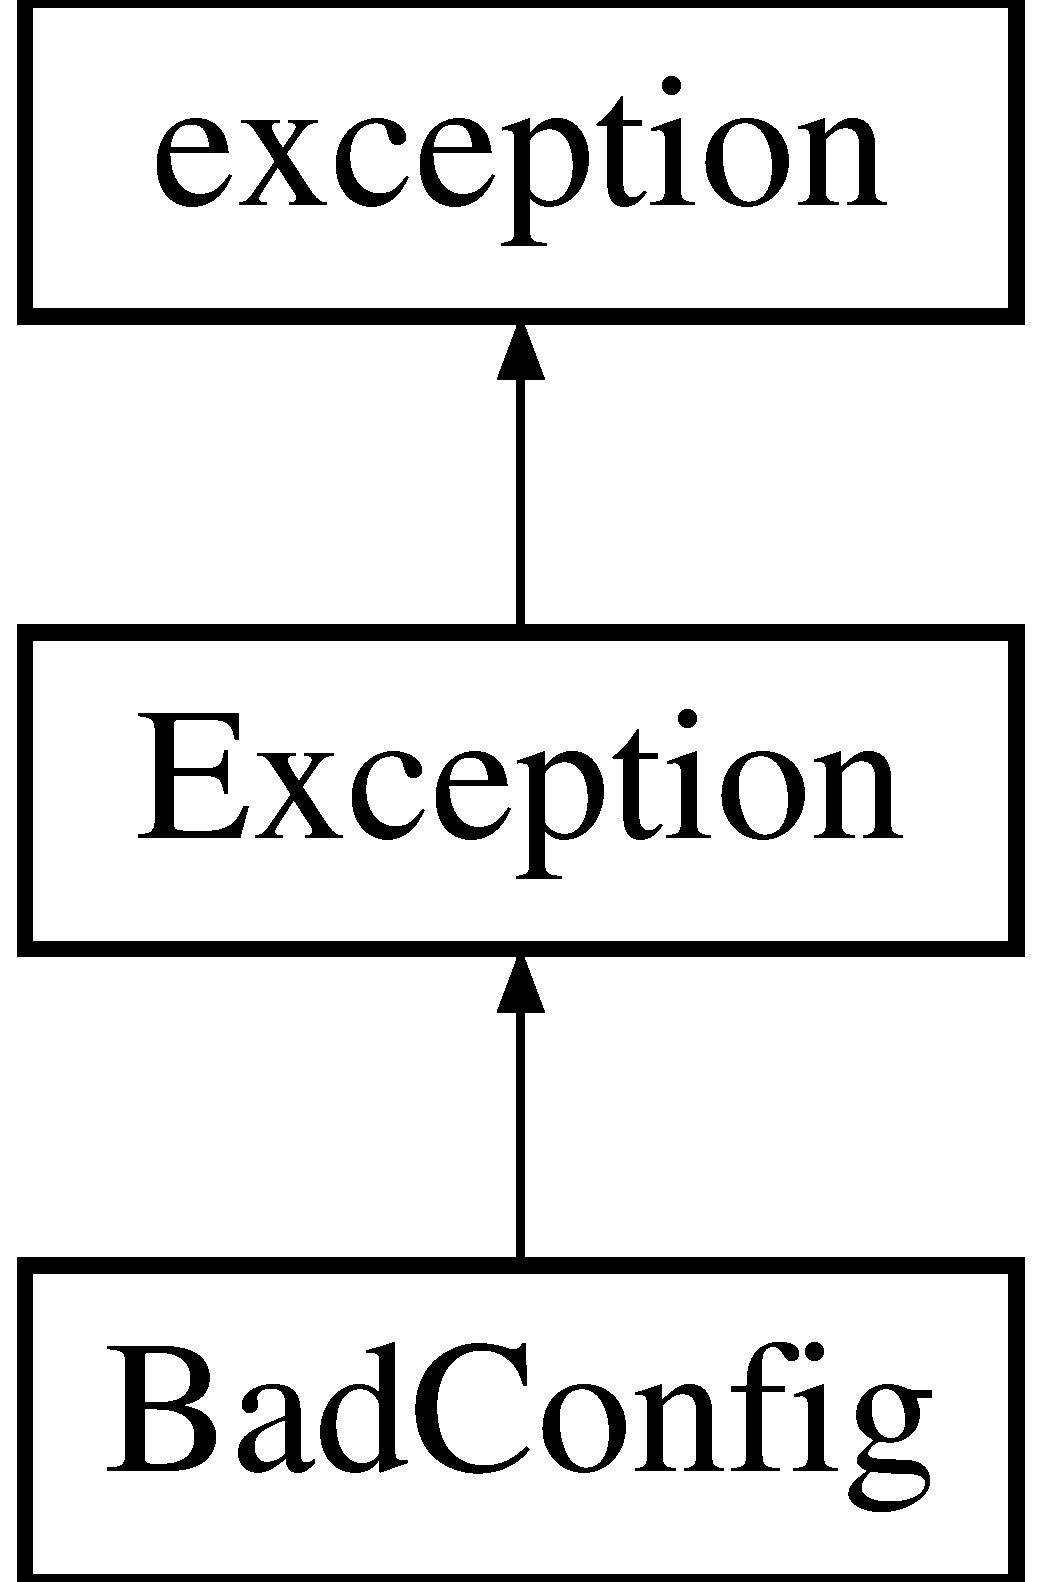
\includegraphics[height=3.000000cm]{class_bad_config}
\end{center}
\end{figure}
\subsection*{Public Member Functions}
\begin{DoxyCompactItemize}
\item 
\hypertarget{class_bad_config_a2f9e1e294d617c65268b36eb7668a1db}{{\bfseries Bad\-Config} (const std\-::string \&error)}\label{class_bad_config_a2f9e1e294d617c65268b36eb7668a1db}

\item 
\hypertarget{class_bad_config_a0fe20153a015ee59c7f7e63f550d99d8}{{\bfseries Bad\-Config} (const char $\ast$error)}\label{class_bad_config_a0fe20153a015ee59c7f7e63f550d99d8}

\end{DoxyCompactItemize}
\subsection*{Additional Inherited Members}


\subsection{Detailed Description}
Config is not complete. 

The documentation for this class was generated from the following file\-:\begin{DoxyCompactItemize}
\item 
Core/Exceptions.\-hpp\end{DoxyCompactItemize}

\hypertarget{class_bad_index}{\section{Bad\-Index Class Reference}
\label{class_bad_index}\index{Bad\-Index@{Bad\-Index}}
}


Index out of range.  




{\ttfamily \#include $<$Exceptions.\-hpp$>$}

Inheritance diagram for Bad\-Index\-:\begin{figure}[H]
\begin{center}
\leavevmode
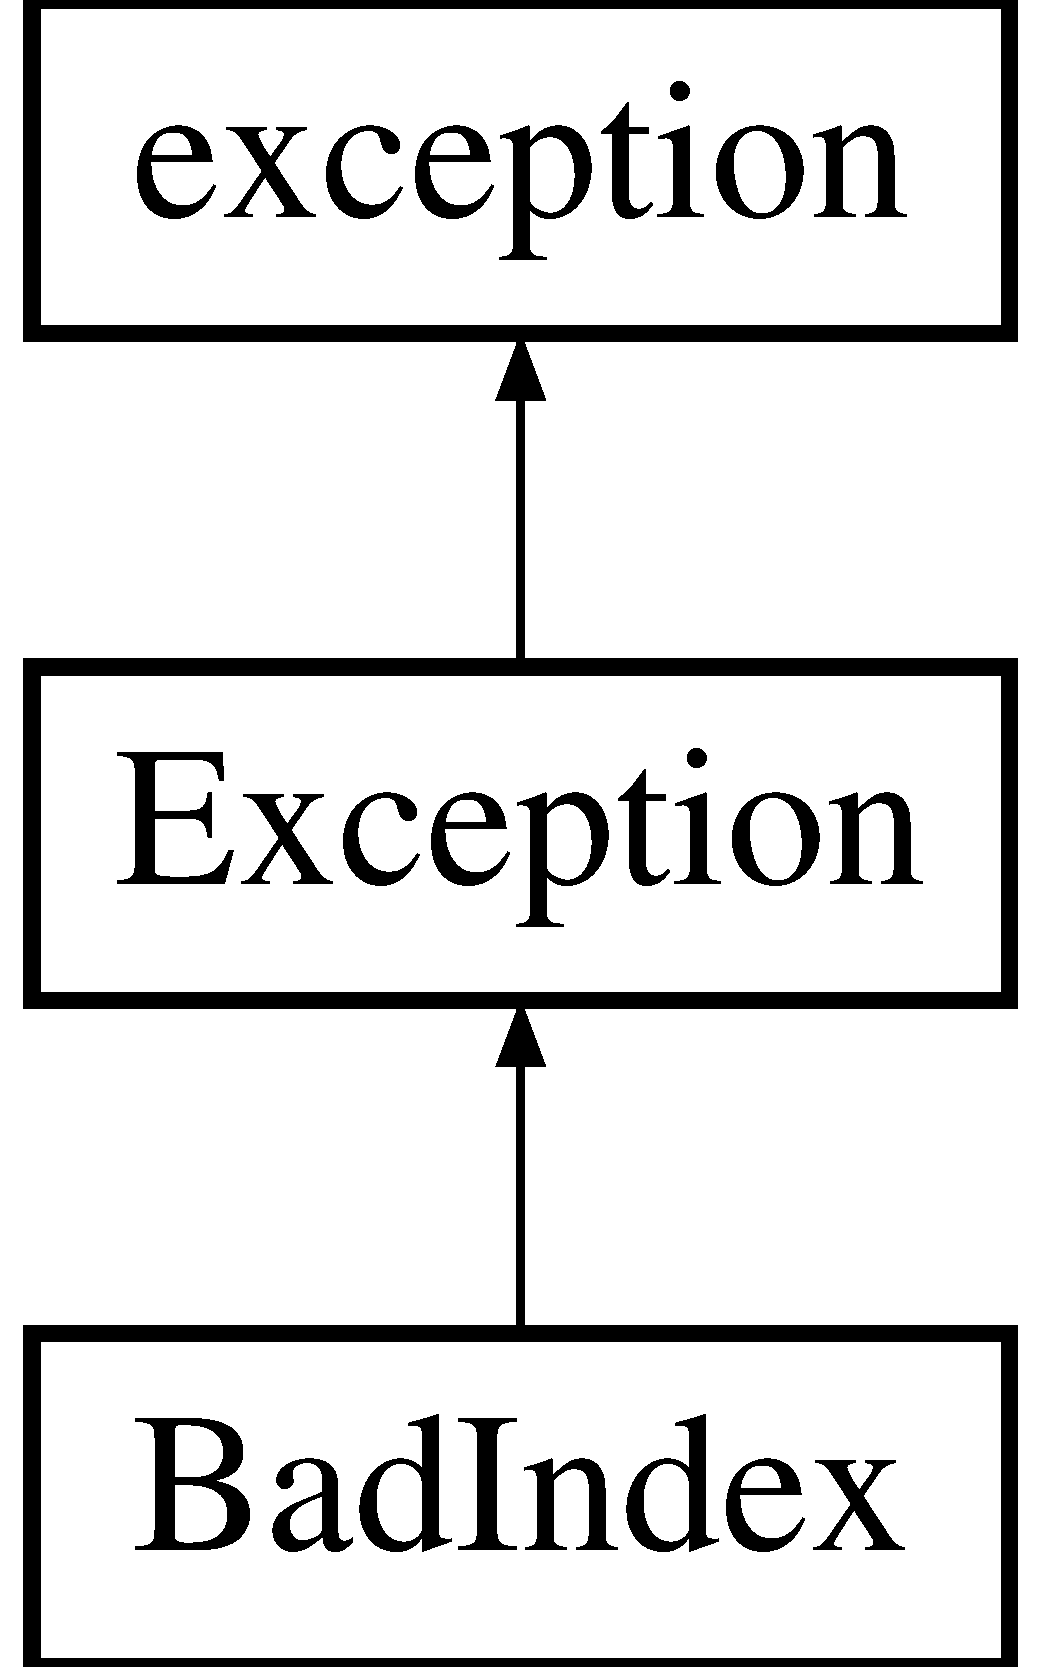
\includegraphics[height=3.000000cm]{class_bad_index}
\end{center}
\end{figure}
\subsection*{Public Member Functions}
\begin{DoxyCompactItemize}
\item 
\hypertarget{class_bad_index_a88772de21dc1a2f4f7cd02c6e9e6c7da}{{\bfseries Bad\-Index} (const std\-::string \&error)}\label{class_bad_index_a88772de21dc1a2f4f7cd02c6e9e6c7da}

\item 
\hypertarget{class_bad_index_a0fea6f97b42a4663e7a162e4c08e556d}{{\bfseries Bad\-Index} (const char $\ast$error)}\label{class_bad_index_a0fea6f97b42a4663e7a162e4c08e556d}

\end{DoxyCompactItemize}
\subsection*{Additional Inherited Members}


\subsection{Detailed Description}
Index out of range. 

The documentation for this class was generated from the following file\-:\begin{DoxyCompactItemize}
\item 
Core/Exceptions.\-hpp\end{DoxyCompactItemize}

\hypertarget{class_bad_parameter}{\section{Bad\-Parameter Class Reference}
\label{class_bad_parameter}\index{Bad\-Parameter@{Bad\-Parameter}}
}


Parameter not existing.  




{\ttfamily \#include $<$Exceptions.\-hpp$>$}

Inheritance diagram for Bad\-Parameter\-:\begin{figure}[H]
\begin{center}
\leavevmode
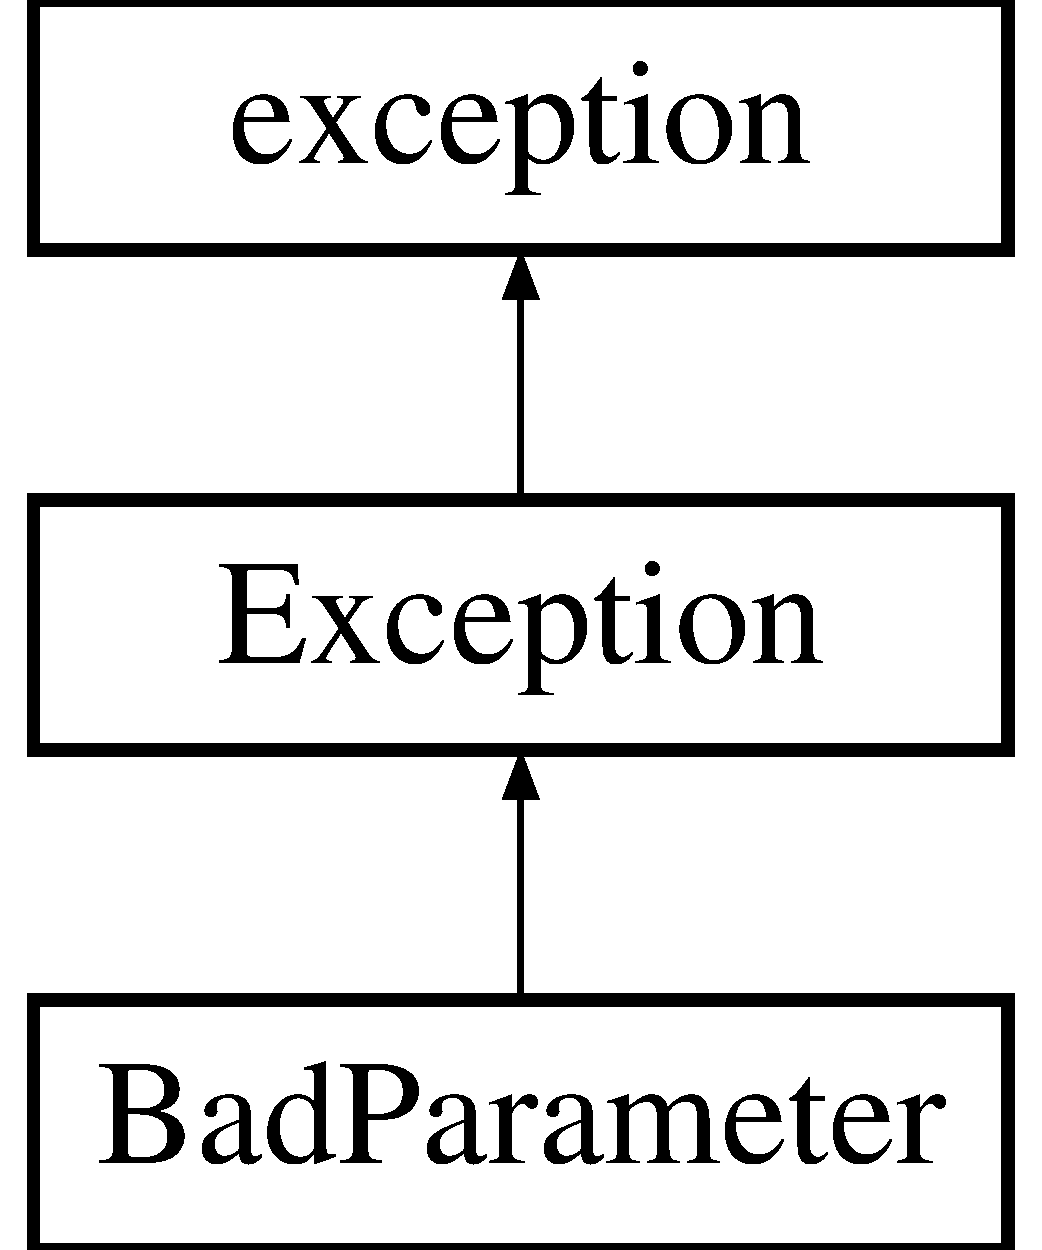
\includegraphics[height=3.000000cm]{class_bad_parameter}
\end{center}
\end{figure}
\subsection*{Public Member Functions}
\begin{DoxyCompactItemize}
\item 
\hypertarget{class_bad_parameter_ae87d4d3bf6936a524a45b97602f369dd}{{\bfseries Bad\-Parameter} (const std\-::string \&error)}\label{class_bad_parameter_ae87d4d3bf6936a524a45b97602f369dd}

\item 
\hypertarget{class_bad_parameter_a0c4e8cab27c070ab04c716001d8083f7}{{\bfseries Bad\-Parameter} (const char $\ast$error)}\label{class_bad_parameter_a0c4e8cab27c070ab04c716001d8083f7}

\end{DoxyCompactItemize}
\subsection*{Additional Inherited Members}


\subsection{Detailed Description}
Parameter not existing. 

The documentation for this class was generated from the following file\-:\begin{DoxyCompactItemize}
\item 
Core/Exceptions.\-hpp\end{DoxyCompactItemize}

\hypertarget{class_bool_parameter}{\section{Bool\-Parameter Class Reference}
\label{class_bool_parameter}\index{Bool\-Parameter@{Bool\-Parameter}}
}
\subsection*{Public Member Functions}
\begin{DoxyCompactItemize}
\item 
\hyperlink{class_bool_parameter_adf6b711da9d2a89ea563c18063456ba4}{Bool\-Parameter} ()
\begin{DoxyCompactList}\small\item\em Standard constructor without information. \end{DoxyCompactList}\item 
\hyperlink{class_bool_parameter_ad71f979faed387cd7107cb6aaeb9d974}{Bool\-Parameter} (const bool value)
\begin{DoxyCompactList}\small\item\em Standard constructor with a value. \end{DoxyCompactList}\item 
\hyperlink{class_bool_parameter_a950a68f3877f07a3089224ba13c5215d}{Bool\-Parameter} (const bool value, const bool error)
\begin{DoxyCompactList}\small\item\em Standard constructor with value and error. \end{DoxyCompactList}\item 
\hyperlink{class_bool_parameter_a60cddb7b3fc1270cb79a238759744259}{Bool\-Parameter} (const \hyperlink{class_bool_parameter}{Bool\-Parameter} \&in)
\begin{DoxyCompactList}\small\item\em Copy constructor using = operator. \end{DoxyCompactList}\item 
virtual \hyperlink{class_bool_parameter_a385490fd59b6d27a9fb1ef63c2ff43bc}{$\sim$\-Bool\-Parameter} ()
\begin{DoxyCompactList}\small\item\em Empty Destructor. \end{DoxyCompactList}\item 
\hypertarget{class_bool_parameter_a25b8a4587ad9e01e3dcfc1ba9067f795}{virtual const bool \hyperlink{class_bool_parameter_a25b8a4587ad9e01e3dcfc1ba9067f795}{Has\-Error} () const }\label{class_bool_parameter_a25b8a4587ad9e01e3dcfc1ba9067f795}

\begin{DoxyCompactList}\small\item\em Check if parameter has an error. \end{DoxyCompactList}\item 
\hypertarget{class_bool_parameter_a280c5f86138bcc626ebb65829b579ff6}{virtual const bool \hyperlink{class_bool_parameter_a280c5f86138bcc626ebb65829b579ff6}{Is\-Fixed} () const }\label{class_bool_parameter_a280c5f86138bcc626ebb65829b579ff6}

\begin{DoxyCompactList}\small\item\em Check if parameter is fixed. \end{DoxyCompactList}\item 
\hypertarget{class_bool_parameter_a90c52946f9a9a137828cecc9caa28bc3}{virtual const bool \hyperlink{class_bool_parameter_a90c52946f9a9a137828cecc9caa28bc3}{Get\-Value} () const }\label{class_bool_parameter_a90c52946f9a9a137828cecc9caa28bc3}

\begin{DoxyCompactList}\small\item\em Getter for value of parameter. \end{DoxyCompactList}\item 
\hypertarget{class_bool_parameter_a3a5271d52e3a04f8528690ab3dddb0d0}{virtual const bool \hyperlink{class_bool_parameter_a3a5271d52e3a04f8528690ab3dddb0d0}{Get\-Error} () const }\label{class_bool_parameter_a3a5271d52e3a04f8528690ab3dddb0d0}

\begin{DoxyCompactList}\small\item\em Getter for error of parameter. \end{DoxyCompactList}\item 
\hypertarget{class_bool_parameter_a6073659d93c392cd6a3f8a603166d693}{virtual void \hyperlink{class_bool_parameter_a6073659d93c392cd6a3f8a603166d693}{Set\-Value} (const bool in\-Val)}\label{class_bool_parameter_a6073659d93c392cd6a3f8a603166d693}

\begin{DoxyCompactList}\small\item\em Setter for value of parameter. \end{DoxyCompactList}\item 
\hypertarget{class_bool_parameter_a61be0c3c228bc957602a3811ea68e6cc}{virtual void \hyperlink{class_bool_parameter_a61be0c3c228bc957602a3811ea68e6cc}{Set\-Error} (const bool in\-Err)}\label{class_bool_parameter_a61be0c3c228bc957602a3811ea68e6cc}

\begin{DoxyCompactList}\small\item\em Setter for error of parameter. \end{DoxyCompactList}\item 
\hypertarget{class_bool_parameter_a651a5ed8154eed589c31b6c93e8538fc}{virtual const void \hyperlink{class_bool_parameter_a651a5ed8154eed589c31b6c93e8538fc}{Set\-Parameter\-Fixed} ()}\label{class_bool_parameter_a651a5ed8154eed589c31b6c93e8538fc}

\begin{DoxyCompactList}\small\item\em Call to fix parameter. \end{DoxyCompactList}\item 
\hypertarget{class_bool_parameter_a048483a4a765ad5b100a19b8d5f1ed49}{virtual const void \hyperlink{class_bool_parameter_a048483a4a765ad5b100a19b8d5f1ed49}{Set\-Parameter\-Free} ()}\label{class_bool_parameter_a048483a4a765ad5b100a19b8d5f1ed49}

\begin{DoxyCompactList}\small\item\em Call to free parameter. \end{DoxyCompactList}\item 
\hypertarget{class_bool_parameter_a827373e73426bc1df9e0504fd05452b6}{virtual const void \hyperlink{class_bool_parameter_a827373e73426bc1df9e0504fd05452b6}{Fix\-Parameter} (const bool fixed)}\label{class_bool_parameter_a827373e73426bc1df9e0504fd05452b6}

\begin{DoxyCompactList}\small\item\em Set parameter free or fixed. \end{DoxyCompactList}\item 
std\-::string const \& \hyperlink{class_bool_parameter_a251a49ae038463171f4d930d3a29a85e}{to\-\_\-str} () const 
\begin{DoxyCompactList}\small\item\em A public function returning a string with parameter information. \end{DoxyCompactList}\item 
virtual const std\-::string \hyperlink{class_bool_parameter_a6721b6ea49385a388b622afdf6b03d59}{type} ()
\begin{DoxyCompactList}\small\item\em A public function returning a string naming its type. \end{DoxyCompactList}\end{DoxyCompactItemize}
\subsection*{Protected Member Functions}
\begin{DoxyCompactItemize}
\item 
virtual void \hyperlink{class_bool_parameter_ad385b85691363fa3a304455f110cb1eb}{make\-\_\-str} ()
\begin{DoxyCompactList}\small\item\em A protected function which creates an output string for printing. \end{DoxyCompactList}\end{DoxyCompactItemize}
\subsection*{Protected Attributes}
\begin{DoxyCompactItemize}
\item 
std\-::string \hyperlink{class_bool_parameter_a836a9f6e5b814156665c2de8c00c31a2}{out\-\_\-}
\item 
bool \hyperlink{class_bool_parameter_a9c192361dd600e72bbf06eee33fa0899}{error\-\_\-}
\item 
bool \hyperlink{class_bool_parameter_a16c8c857c4c9cd45714e7858b41f55f2}{usebounds\-\_\-}
\item 
bool \hyperlink{class_bool_parameter_acaa36aae968e133f21b2cebb6216dee9}{fixed\-\_\-}
\item 
\hypertarget{class_bool_parameter_a5ac86e1f505fad22eeea171bcc8748c9}{int {\bfseries val\-\_\-}}\label{class_bool_parameter_a5ac86e1f505fad22eeea171bcc8748c9}

\item 
int \hyperlink{class_bool_parameter_a21d7587dbe2a95be0329ef9933ff041d}{err\-\_\-}
\end{DoxyCompactItemize}
\subsection*{Friends}
\begin{DoxyCompactItemize}
\item 
std\-::ostream \& \hyperlink{class_bool_parameter_a5239796d0d37d86b7003f4337efe920a}{operator$<$$<$} (std\-::ostream \&os, const \hyperlink{class_bool_parameter}{Bool\-Parameter} \&p)
\begin{DoxyCompactList}\small\item\em friend function to stream parameter information to output \end{DoxyCompactList}\end{DoxyCompactItemize}


\subsection{Constructor \& Destructor Documentation}
\hypertarget{class_bool_parameter_adf6b711da9d2a89ea563c18063456ba4}{\index{Bool\-Parameter@{Bool\-Parameter}!Bool\-Parameter@{Bool\-Parameter}}
\index{Bool\-Parameter@{Bool\-Parameter}!BoolParameter@{Bool\-Parameter}}
\subsubsection[{Bool\-Parameter}]{\setlength{\rightskip}{0pt plus 5cm}Bool\-Parameter\-::\-Bool\-Parameter (
\begin{DoxyParamCaption}
{}
\end{DoxyParamCaption}
)\hspace{0.3cm}{\ttfamily [inline]}}}\label{class_bool_parameter_adf6b711da9d2a89ea563c18063456ba4}


Standard constructor without information. 

Standard constructor with no information provided. Creates parameter with value 0 but without bounds or an error. \begin{DoxySeeAlso}{See Also}
\hyperlink{class_bool_parameter_ad385b85691363fa3a304455f110cb1eb}{make\-\_\-str()} 
\end{DoxySeeAlso}
\hypertarget{class_bool_parameter_ad71f979faed387cd7107cb6aaeb9d974}{\index{Bool\-Parameter@{Bool\-Parameter}!Bool\-Parameter@{Bool\-Parameter}}
\index{Bool\-Parameter@{Bool\-Parameter}!BoolParameter@{Bool\-Parameter}}
\subsubsection[{Bool\-Parameter}]{\setlength{\rightskip}{0pt plus 5cm}Bool\-Parameter\-::\-Bool\-Parameter (
\begin{DoxyParamCaption}
\item[{const bool}]{value}
\end{DoxyParamCaption}
)\hspace{0.3cm}{\ttfamily [inline]}}}\label{class_bool_parameter_ad71f979faed387cd7107cb6aaeb9d974}


Standard constructor with a value. 

Standard constructor with just a value provided. Creates parameter with given value but without bounds or an error. 
\begin{DoxyParams}{Parameters}
{\em value} & input value of the parameter \\
\hline
\end{DoxyParams}
\begin{DoxySeeAlso}{See Also}
\hyperlink{class_bool_parameter_ad385b85691363fa3a304455f110cb1eb}{make\-\_\-str()} 
\end{DoxySeeAlso}
\hypertarget{class_bool_parameter_a950a68f3877f07a3089224ba13c5215d}{\index{Bool\-Parameter@{Bool\-Parameter}!Bool\-Parameter@{Bool\-Parameter}}
\index{Bool\-Parameter@{Bool\-Parameter}!BoolParameter@{Bool\-Parameter}}
\subsubsection[{Bool\-Parameter}]{\setlength{\rightskip}{0pt plus 5cm}Bool\-Parameter\-::\-Bool\-Parameter (
\begin{DoxyParamCaption}
\item[{const bool}]{value, }
\item[{const bool}]{error}
\end{DoxyParamCaption}
)\hspace{0.3cm}{\ttfamily [inline]}}}\label{class_bool_parameter_a950a68f3877f07a3089224ba13c5215d}


Standard constructor with value and error. 

Standard constructor with value and error provided. Creates parameter with given value and error but without bounds. 
\begin{DoxyParams}{Parameters}
{\em value} & input value of the parameter \\
\hline
{\em error} & input error of the parameter \\
\hline
\end{DoxyParams}
\begin{DoxySeeAlso}{See Also}
\hyperlink{class_bool_parameter_ad385b85691363fa3a304455f110cb1eb}{make\-\_\-str()} 
\end{DoxySeeAlso}
\hypertarget{class_bool_parameter_a60cddb7b3fc1270cb79a238759744259}{\index{Bool\-Parameter@{Bool\-Parameter}!Bool\-Parameter@{Bool\-Parameter}}
\index{Bool\-Parameter@{Bool\-Parameter}!BoolParameter@{Bool\-Parameter}}
\subsubsection[{Bool\-Parameter}]{\setlength{\rightskip}{0pt plus 5cm}Bool\-Parameter\-::\-Bool\-Parameter (
\begin{DoxyParamCaption}
\item[{const {\bf Bool\-Parameter} \&}]{in}
\end{DoxyParamCaption}
)\hspace{0.3cm}{\ttfamily [inline]}}}\label{class_bool_parameter_a60cddb7b3fc1270cb79a238759744259}


Copy constructor using = operator. 

Simple copy constructor using the = operator. As this operator is not overloaded in this class, c++ will copy every member variable. As this is a container class, this should be fine. 
\begin{DoxyParams}{Parameters}
{\em in} & input P\-W\-A\-Parameter which variables will be copied \\
\hline
\end{DoxyParams}
\hypertarget{class_bool_parameter_a385490fd59b6d27a9fb1ef63c2ff43bc}{\index{Bool\-Parameter@{Bool\-Parameter}!$\sim$\-Bool\-Parameter@{$\sim$\-Bool\-Parameter}}
\index{$\sim$\-Bool\-Parameter@{$\sim$\-Bool\-Parameter}!BoolParameter@{Bool\-Parameter}}
\subsubsection[{$\sim$\-Bool\-Parameter}]{\setlength{\rightskip}{0pt plus 5cm}virtual Bool\-Parameter\-::$\sim$\-Bool\-Parameter (
\begin{DoxyParamCaption}
{}
\end{DoxyParamCaption}
)\hspace{0.3cm}{\ttfamily [inline]}, {\ttfamily [virtual]}}}\label{class_bool_parameter_a385490fd59b6d27a9fb1ef63c2ff43bc}


Empty Destructor. 

There is nothing to destroy \-:( 

\subsection{Member Function Documentation}
\hypertarget{class_bool_parameter_ad385b85691363fa3a304455f110cb1eb}{\index{Bool\-Parameter@{Bool\-Parameter}!make\-\_\-str@{make\-\_\-str}}
\index{make\-\_\-str@{make\-\_\-str}!BoolParameter@{Bool\-Parameter}}
\subsubsection[{make\-\_\-str}]{\setlength{\rightskip}{0pt plus 5cm}virtual void Bool\-Parameter\-::make\-\_\-str (
\begin{DoxyParamCaption}
{}
\end{DoxyParamCaption}
)\hspace{0.3cm}{\ttfamily [inline]}, {\ttfamily [protected]}, {\ttfamily [virtual]}}}\label{class_bool_parameter_ad385b85691363fa3a304455f110cb1eb}


A protected function which creates an output string for printing. 

This function uses all available information about the parameter to create a string which will be streamed via the stream operator $<$$<$. \begin{DoxySeeAlso}{See Also}
operator$<$$<$, \hyperlink{class_bool_parameter_a251a49ae038463171f4d930d3a29a85e}{to\-\_\-str()}, \hyperlink{class_bool_parameter_a6721b6ea49385a388b622afdf6b03d59}{type()} 
\end{DoxySeeAlso}
\hypertarget{class_bool_parameter_a251a49ae038463171f4d930d3a29a85e}{\index{Bool\-Parameter@{Bool\-Parameter}!to\-\_\-str@{to\-\_\-str}}
\index{to\-\_\-str@{to\-\_\-str}!BoolParameter@{Bool\-Parameter}}
\subsubsection[{to\-\_\-str}]{\setlength{\rightskip}{0pt plus 5cm}std\-::string const\& Bool\-Parameter\-::to\-\_\-str (
\begin{DoxyParamCaption}
{}
\end{DoxyParamCaption}
) const\hspace{0.3cm}{\ttfamily [inline]}}}\label{class_bool_parameter_a251a49ae038463171f4d930d3a29a85e}


A public function returning a string with parameter information. 

This function simply returns the member string out\-\_\-, which contains all parameter information. The string gets rebuild with every change of the parameter. \begin{DoxyReturn}{Returns}
string with parameter information 
\end{DoxyReturn}
\begin{DoxySeeAlso}{See Also}
operator$<$$<$, \hyperlink{class_bool_parameter_ad385b85691363fa3a304455f110cb1eb}{make\-\_\-str()} 
\end{DoxySeeAlso}
\hypertarget{class_bool_parameter_a6721b6ea49385a388b622afdf6b03d59}{\index{Bool\-Parameter@{Bool\-Parameter}!type@{type}}
\index{type@{type}!BoolParameter@{Bool\-Parameter}}
\subsubsection[{type}]{\setlength{\rightskip}{0pt plus 5cm}virtual const std\-::string Bool\-Parameter\-::type (
\begin{DoxyParamCaption}
{}
\end{DoxyParamCaption}
)\hspace{0.3cm}{\ttfamily [inline]}, {\ttfamily [virtual]}}}\label{class_bool_parameter_a6721b6ea49385a388b622afdf6b03d59}


A public function returning a string naming its type. 

This function is used to get the type of the implementation of this general parameter interface. \begin{DoxySeeAlso}{See Also}
operator$<$$<$, \hyperlink{class_bool_parameter_a251a49ae038463171f4d930d3a29a85e}{to\-\_\-str()}, \hyperlink{class_bool_parameter_ad385b85691363fa3a304455f110cb1eb}{make\-\_\-str()} 
\end{DoxySeeAlso}


\subsection{Friends And Related Function Documentation}
\hypertarget{class_bool_parameter_a5239796d0d37d86b7003f4337efe920a}{\index{Bool\-Parameter@{Bool\-Parameter}!operator$<$$<$@{operator$<$$<$}}
\index{operator$<$$<$@{operator$<$$<$}!BoolParameter@{Bool\-Parameter}}
\subsubsection[{operator$<$$<$}]{\setlength{\rightskip}{0pt plus 5cm}std\-::ostream\& operator$<$$<$ (
\begin{DoxyParamCaption}
\item[{std\-::ostream \&}]{os, }
\item[{const {\bf Bool\-Parameter} \&}]{p}
\end{DoxyParamCaption}
)\hspace{0.3cm}{\ttfamily [friend]}}}\label{class_bool_parameter_a5239796d0d37d86b7003f4337efe920a}


friend function to stream parameter information to output 

Declaring the stream-\/operator $<$$<$ as friend allows to stream parameter information to the output as easily as a generic type. The definition of this class has to be outside the namespace of the class. \begin{DoxySeeAlso}{See Also}
\hyperlink{class_bool_parameter_ad385b85691363fa3a304455f110cb1eb}{make\-\_\-str()}, \hyperlink{class_bool_parameter_a251a49ae038463171f4d930d3a29a85e}{to\-\_\-str()} 
\end{DoxySeeAlso}


\subsection{Field Documentation}
\hypertarget{class_bool_parameter_a21d7587dbe2a95be0329ef9933ff041d}{\index{Bool\-Parameter@{Bool\-Parameter}!err\-\_\-@{err\-\_\-}}
\index{err\-\_\-@{err\-\_\-}!BoolParameter@{Bool\-Parameter}}
\subsubsection[{err\-\_\-}]{\setlength{\rightskip}{0pt plus 5cm}int Bool\-Parameter\-::err\-\_\-\hspace{0.3cm}{\ttfamily [protected]}}}\label{class_bool_parameter_a21d7587dbe2a95be0329ef9933ff041d}
Containers of parameter information \hypertarget{class_bool_parameter_a9c192361dd600e72bbf06eee33fa0899}{\index{Bool\-Parameter@{Bool\-Parameter}!error\-\_\-@{error\-\_\-}}
\index{error\-\_\-@{error\-\_\-}!BoolParameter@{Bool\-Parameter}}
\subsubsection[{error\-\_\-}]{\setlength{\rightskip}{0pt plus 5cm}bool Bool\-Parameter\-::error\-\_\-\hspace{0.3cm}{\ttfamily [protected]}}}\label{class_bool_parameter_a9c192361dd600e72bbf06eee33fa0899}
Is an error defined for this parameter? \hypertarget{class_bool_parameter_acaa36aae968e133f21b2cebb6216dee9}{\index{Bool\-Parameter@{Bool\-Parameter}!fixed\-\_\-@{fixed\-\_\-}}
\index{fixed\-\_\-@{fixed\-\_\-}!BoolParameter@{Bool\-Parameter}}
\subsubsection[{fixed\-\_\-}]{\setlength{\rightskip}{0pt plus 5cm}bool Bool\-Parameter\-::fixed\-\_\-\hspace{0.3cm}{\ttfamily [protected]}}}\label{class_bool_parameter_acaa36aae968e133f21b2cebb6216dee9}
Do you want to keep parameter fixed? \hypertarget{class_bool_parameter_a836a9f6e5b814156665c2de8c00c31a2}{\index{Bool\-Parameter@{Bool\-Parameter}!out\-\_\-@{out\-\_\-}}
\index{out\-\_\-@{out\-\_\-}!BoolParameter@{Bool\-Parameter}}
\subsubsection[{out\-\_\-}]{\setlength{\rightskip}{0pt plus 5cm}std\-::string Bool\-Parameter\-::out\-\_\-\hspace{0.3cm}{\ttfamily [protected]}}}\label{class_bool_parameter_a836a9f6e5b814156665c2de8c00c31a2}
Output string to print information \hypertarget{class_bool_parameter_a16c8c857c4c9cd45714e7858b41f55f2}{\index{Bool\-Parameter@{Bool\-Parameter}!usebounds\-\_\-@{usebounds\-\_\-}}
\index{usebounds\-\_\-@{usebounds\-\_\-}!BoolParameter@{Bool\-Parameter}}
\subsubsection[{usebounds\-\_\-}]{\setlength{\rightskip}{0pt plus 5cm}bool Bool\-Parameter\-::usebounds\-\_\-\hspace{0.3cm}{\ttfamily [protected]}}}\label{class_bool_parameter_a16c8c857c4c9cd45714e7858b41f55f2}
Do you want to restrict your parameter? 

The documentation for this class was generated from the following file\-:\begin{DoxyCompactItemize}
\item 
Core/\hyperlink{_parameter_8hpp}{Parameter.\-hpp}\end{DoxyCompactItemize}

\hypertarget{class_breit_wigner}{\section{Breit\-Wigner Class Reference}
\label{class_breit_wigner}\index{Breit\-Wigner@{Breit\-Wigner}}
}


Physics Module with simple 1\-D Breit-\/\-Wigner.  




{\ttfamily \#include $<$Breit\-Wigner.\-hpp$>$}

Inheritance diagram for Breit\-Wigner\-:\begin{figure}[H]
\begin{center}
\leavevmode
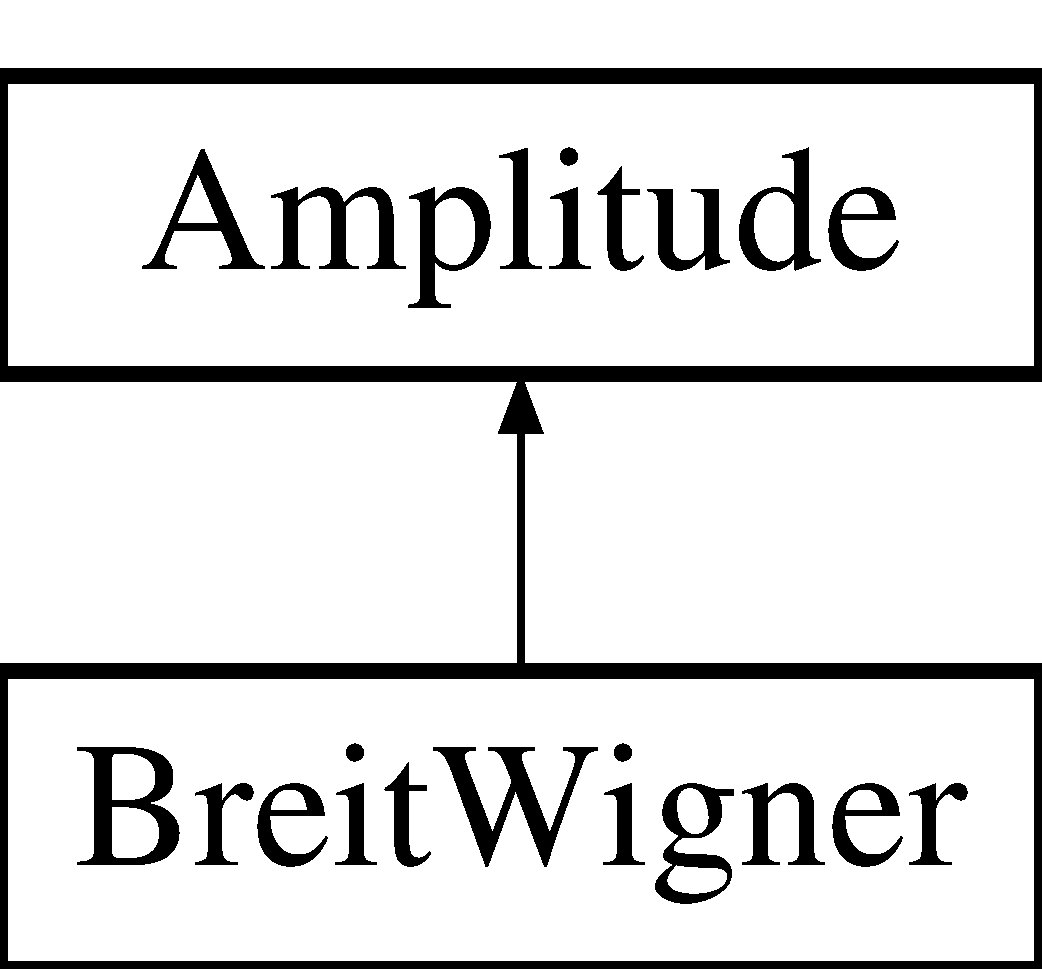
\includegraphics[height=2.000000cm]{class_breit_wigner}
\end{center}
\end{figure}
\subsection*{Public Member Functions}
\begin{DoxyCompactItemize}
\item 
\hypertarget{class_breit_wigner_a3b4a7cb3e7565729dc493ac8387d8278}{\hyperlink{class_breit_wigner_a3b4a7cb3e7565729dc493ac8387d8278}{Breit\-Wigner} (const double min, const double max)}\label{class_breit_wigner_a3b4a7cb3e7565729dc493ac8387d8278}

\begin{DoxyCompactList}\small\item\em Default Constructor (0x0) \end{DoxyCompactList}\item 
\hypertarget{class_breit_wigner_a9d73071fd70cc2ca0ce1e566a3d3127c}{virtual const double {\bfseries integral} (\hyperlink{class_parameter_list}{Parameter\-List} \&par)}\label{class_breit_wigner_a9d73071fd70cc2ca0ce1e566a3d3127c}

\item 
\hypertarget{class_breit_wigner_a7d352fe9651163d4ca8ed35de06827b8}{virtual const double {\bfseries draw\-Int} (double $\ast$x, double $\ast$p)}\label{class_breit_wigner_a7d352fe9651163d4ca8ed35de06827b8}

\item 
\hypertarget{class_breit_wigner_a2bebe3d32b95d04ac730ebe04262f9ff}{virtual const double {\bfseries intensity} (double x, double M, double T)}\label{class_breit_wigner_a2bebe3d32b95d04ac730ebe04262f9ff}

\item 
\hypertarget{class_breit_wigner_a3528a7b3c2bca11a338c1e04707bc817}{virtual const double {\bfseries intensity} (std\-::vector$<$ double $>$ \&x, \hyperlink{class_parameter_list}{Parameter\-List} \&par)}\label{class_breit_wigner_a3528a7b3c2bca11a338c1e04707bc817}

\item 
\hypertarget{class_breit_wigner_a722422da4ac4be5e7706b21e98b74b10}{virtual const bool {\bfseries fill\-Start\-Par\-Vec} (\hyperlink{class_parameter_list}{Parameter\-List} \&out\-Par)}\label{class_breit_wigner_a722422da4ac4be5e7706b21e98b74b10}

\item 
\hypertarget{class_breit_wigner_a54591629d2b9c6bdeb241c50c6670c64}{virtual void {\bfseries print\-Amps} ()}\label{class_breit_wigner_a54591629d2b9c6bdeb241c50c6670c64}

\item 
\hypertarget{class_breit_wigner_a14309665b47fb14b7e89019b6103b17e}{virtual double {\bfseries get\-Max\-Val} ()}\label{class_breit_wigner_a14309665b47fb14b7e89019b6103b17e}

\item 
virtual \hyperlink{class_breit_wigner_abf5cae715df95e2962de1255551751db}{$\sim$\-Breit\-Wigner} ()
\end{DoxyCompactItemize}
\subsection*{Protected Attributes}
\begin{DoxyCompactItemize}
\item 
\hypertarget{class_breit_wigner_ae082a9df35a4cdcf7d2a3bbe87553013}{double {\bfseries min\-\_\-}}\label{class_breit_wigner_ae082a9df35a4cdcf7d2a3bbe87553013}

\item 
\hypertarget{class_breit_wigner_a224a6f81765cf77c808e76b6484659aa}{double {\bfseries max\-\_\-}}\label{class_breit_wigner_a224a6f81765cf77c808e76b6484659aa}

\end{DoxyCompactItemize}


\subsection{Detailed Description}
Physics Module with simple 1\-D Breit-\/\-Wigner. 

\subsection{Constructor \& Destructor Documentation}
\hypertarget{class_breit_wigner_abf5cae715df95e2962de1255551751db}{\index{Breit\-Wigner@{Breit\-Wigner}!$\sim$\-Breit\-Wigner@{$\sim$\-Breit\-Wigner}}
\index{$\sim$\-Breit\-Wigner@{$\sim$\-Breit\-Wigner}!BreitWigner@{Breit\-Wigner}}
\subsubsection[{$\sim$\-Breit\-Wigner}]{\setlength{\rightskip}{0pt plus 5cm}Breit\-Wigner\-::$\sim$\-Breit\-Wigner (
\begin{DoxyParamCaption}
{}
\end{DoxyParamCaption}
)\hspace{0.3cm}{\ttfamily [virtual]}}}\label{class_breit_wigner_abf5cae715df95e2962de1255551751db}
Destructor 

The documentation for this class was generated from the following files\-:\begin{DoxyCompactItemize}
\item 
Physics/\-Breit\-Wigner/\hyperlink{_breit_wigner_8hpp}{Breit\-Wigner.\-hpp}\item 
Physics/\-Breit\-Wigner/Breit\-Wigner.\-cpp\end{DoxyCompactItemize}

\hypertarget{class_chi_one_d}{\section{Chi\-One\-D Class Reference}
\label{class_chi_one_d}\index{Chi\-One\-D@{Chi\-One\-D}}
}


Simple $\chi^{2}$-\/\-Estimator.  




{\ttfamily \#include $<$Chi\-One\-D.\-hpp$>$}

Inheritance diagram for Chi\-One\-D\-:\begin{figure}[H]
\begin{center}
\leavevmode
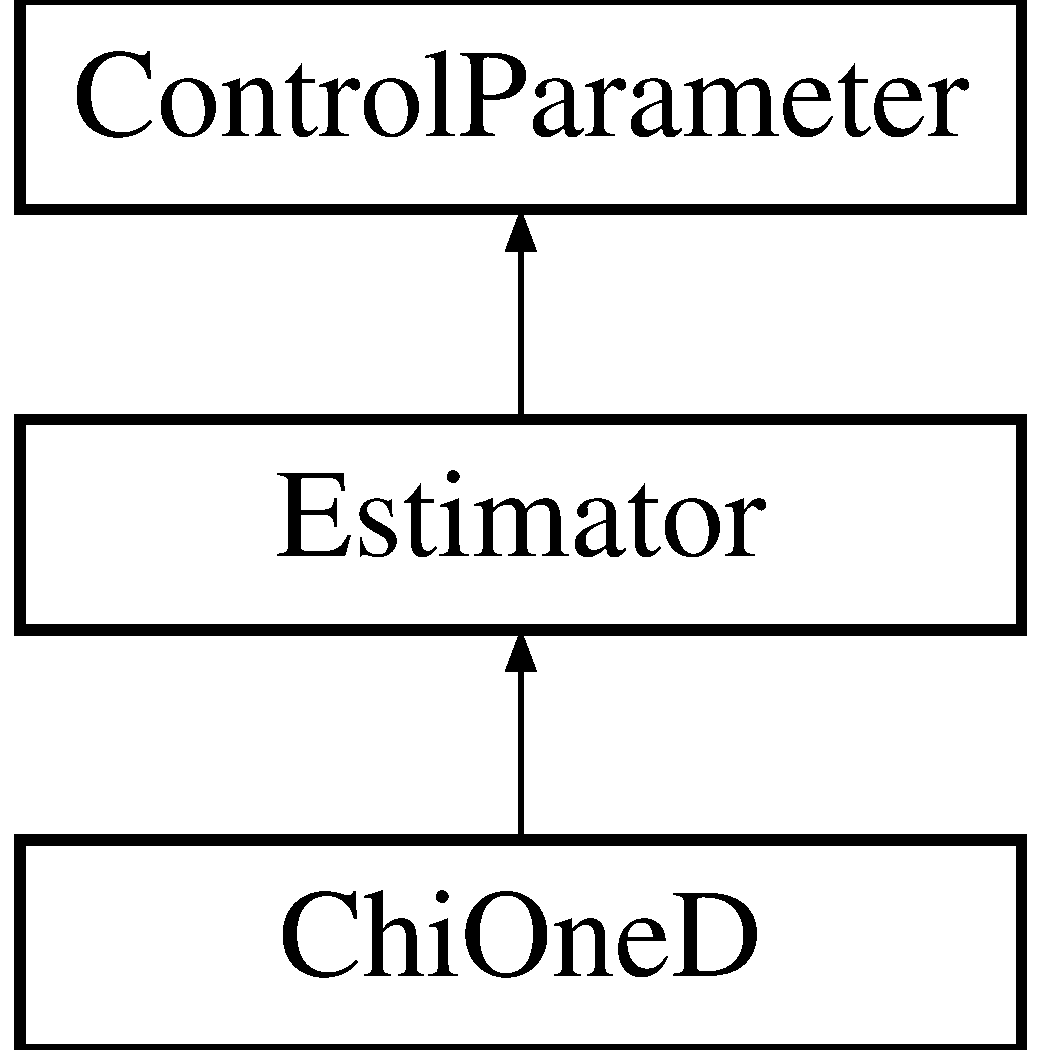
\includegraphics[height=3.000000cm]{class_chi_one_d}
\end{center}
\end{figure}
\subsection*{Public Member Functions}
\begin{DoxyCompactItemize}
\item 
\hypertarget{class_chi_one_d_a01aed70ef28801d04721b8c5068faa15}{virtual double {\bfseries control\-Parameter} (\hyperlink{class_parameter_list}{Parameter\-List} \&min\-Par)}\label{class_chi_one_d_a01aed70ef28801d04721b8c5068faa15}

\item 
virtual \hyperlink{class_chi_one_d_a3e6fd195228f39afb011928f22db5f6e}{$\sim$\-Chi\-One\-D} ()
\end{DoxyCompactItemize}
\subsection*{Static Public Member Functions}
\begin{DoxyCompactItemize}
\item 
\hypertarget{class_chi_one_d_a86bfdd98afdd2fb5b8c95354cd362988}{static std\-::shared\-\_\-ptr\\*
$<$ \hyperlink{class_control_parameter}{Control\-Parameter} $>$ {\bfseries create\-Instance} (std\-::shared\-\_\-ptr$<$ \hyperlink{class_amplitude}{Amplitude} $>$, std\-::shared\-\_\-ptr$<$ \hyperlink{class_data}{Data} $>$)}\label{class_chi_one_d_a86bfdd98afdd2fb5b8c95354cd362988}

\end{DoxyCompactItemize}
\subsection*{Protected Member Functions}
\begin{DoxyCompactItemize}
\item 
\hypertarget{class_chi_one_d_ad203f6ca561b616484a5ff921c1a4b1c}{\hyperlink{class_chi_one_d_ad203f6ca561b616484a5ff921c1a4b1c}{Chi\-One\-D} (std\-::shared\-\_\-ptr$<$ \hyperlink{class_amplitude}{Amplitude} $>$, std\-::shared\-\_\-ptr$<$ \hyperlink{class_data}{Data} $>$)}\label{class_chi_one_d_ad203f6ca561b616484a5ff921c1a4b1c}

\begin{DoxyCompactList}\small\item\em Default Constructor (0x0) \end{DoxyCompactList}\end{DoxyCompactItemize}
\subsection*{Additional Inherited Members}


\subsection{Detailed Description}
Simple $\chi^{2}$-\/\-Estimator. 

\subsection{Constructor \& Destructor Documentation}
\hypertarget{class_chi_one_d_a3e6fd195228f39afb011928f22db5f6e}{\index{Chi\-One\-D@{Chi\-One\-D}!$\sim$\-Chi\-One\-D@{$\sim$\-Chi\-One\-D}}
\index{$\sim$\-Chi\-One\-D@{$\sim$\-Chi\-One\-D}!ChiOneD@{Chi\-One\-D}}
\subsubsection[{$\sim$\-Chi\-One\-D}]{\setlength{\rightskip}{0pt plus 5cm}Chi\-One\-D\-::$\sim$\-Chi\-One\-D (
\begin{DoxyParamCaption}
{}
\end{DoxyParamCaption}
)\hspace{0.3cm}{\ttfamily [virtual]}}}\label{class_chi_one_d_a3e6fd195228f39afb011928f22db5f6e}
Destructor 

The documentation for this class was generated from the following files\-:\begin{DoxyCompactItemize}
\item 
Estimator/\-Chi\-One\-D/\hyperlink{_chi_one_d_8hpp}{Chi\-One\-D.\-hpp}\item 
Estimator/\-Chi\-One\-D/Chi\-One\-D.\-cpp\end{DoxyCompactItemize}

\hypertarget{class_control_parameter}{\section{Control\-Parameter Class Reference}
\label{class_control_parameter}\index{Control\-Parameter@{Control\-Parameter}}
}


\hyperlink{class_optimizer}{Optimizer} \hyperlink{class_data}{Data} Base-\/\-Class.  




{\ttfamily \#include $<$Control\-Parameter.\-hpp$>$}

Inheritance diagram for Control\-Parameter\-:\begin{figure}[H]
\begin{center}
\leavevmode
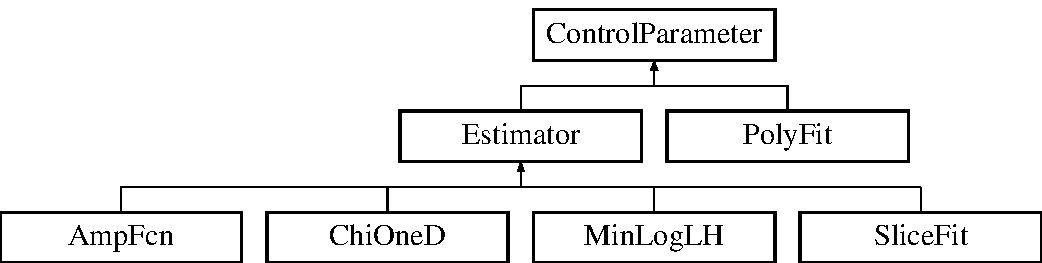
\includegraphics[height=3.000000cm]{class_control_parameter}
\end{center}
\end{figure}
\subsection*{Public Member Functions}
\begin{DoxyCompactItemize}
\item 
\hypertarget{class_control_parameter_ab3d70358bfdcf2419b501cdb8f95d382}{virtual double {\bfseries control\-Parameter} (\hyperlink{class_parameter_list}{Parameter\-List} \&min\-Par)=0}\label{class_control_parameter_ab3d70358bfdcf2419b501cdb8f95d382}

\end{DoxyCompactItemize}
\subsection*{Static Public Member Functions}
\begin{DoxyCompactItemize}
\item 
\hypertarget{class_control_parameter_a8c58559a3358f4b7a5caeeb4a4e98b5d}{static std\-::shared\-\_\-ptr\\*
$<$ \hyperlink{class_control_parameter}{Control\-Parameter} $>$ {\bfseries Instance} ()}\label{class_control_parameter_a8c58559a3358f4b7a5caeeb4a4e98b5d}

\end{DoxyCompactItemize}
\subsection*{Static Protected Attributes}
\begin{DoxyCompactItemize}
\item 
\hypertarget{class_control_parameter_a0e8240e3b7bc2300a9015a82751c72a6}{static std\-::shared\-\_\-ptr\\*
$<$ \hyperlink{class_control_parameter}{Control\-Parameter} $>$ {\bfseries instance\-\_\-} = std\-::shared\-\_\-ptr$<$\hyperlink{class_control_parameter}{Control\-Parameter}$>$()}\label{class_control_parameter_a0e8240e3b7bc2300a9015a82751c72a6}

\end{DoxyCompactItemize}


\subsection{Detailed Description}
\hyperlink{class_optimizer}{Optimizer} \hyperlink{class_data}{Data} Base-\/\-Class. 

The documentation for this class was generated from the following files\-:\begin{DoxyCompactItemize}
\item 
Optimizer/\hyperlink{_control_parameter_8hpp}{Control\-Parameter.\-hpp}\item 
Optimizer/Control\-Parameter.\-cpp\end{DoxyCompactItemize}

\hypertarget{class_data}{\section{Data Class Reference}
\label{class_data}\index{Data@{Data}}
}


\hyperlink{class_data}{Data} Interface Base-\/\-Class.  




{\ttfamily \#include $<$Data.\-hpp$>$}

Inheritance diagram for Data\-:\begin{figure}[H]
\begin{center}
\leavevmode
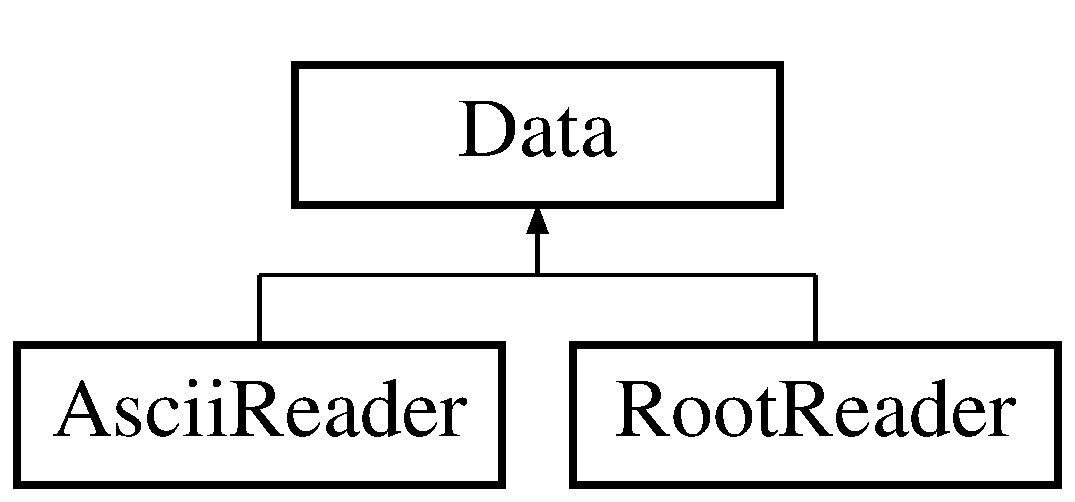
\includegraphics[height=2.000000cm]{class_data}
\end{center}
\end{figure}
\subsection*{Public Member Functions}
\begin{DoxyCompactItemize}
\item 
\hypertarget{class_data_afb361904284b3ec7f7ee365be9202661}{virtual const std\-::vector\\*
$<$ std\-::string $>$ \& {\bfseries get\-Variable\-Names} ()=0}\label{class_data_afb361904284b3ec7f7ee365be9202661}

\item 
\hypertarget{class_data_ab25e52c1eb80f21d49a10258f168e9c9}{virtual const \hyperlink{class_event}{Event} \& {\bfseries get\-Event} (const int)=0}\label{class_data_ab25e52c1eb80f21d49a10258f168e9c9}

\item 
\hypertarget{class_data_af019d4356edf7f4933deb46f4b12fcc1}{virtual const int {\bfseries get\-Bin} (const int, double \&, double \&)=0}\label{class_data_af019d4356edf7f4933deb46f4b12fcc1}

\item 
\hypertarget{class_data_acb735a761c1b22b273ee19f577438d1a}{virtual const unsigned int {\bfseries get\-N\-Events} () const =0}\label{class_data_acb735a761c1b22b273ee19f577438d1a}

\item 
\hypertarget{class_data_aaaad8bb5a7243e3d3ba299acf1fde4fb}{virtual const unsigned int {\bfseries get\-N\-Bins} () const =0}\label{class_data_aaaad8bb5a7243e3d3ba299acf1fde4fb}

\end{DoxyCompactItemize}


\subsection{Detailed Description}
\hyperlink{class_data}{Data} Interface Base-\/\-Class. 

The documentation for this class was generated from the following file\-:\begin{DoxyCompactItemize}
\item 
Data\-Reader/\hyperlink{_data_8hpp}{Data.\-hpp}\end{DoxyCompactItemize}

\hypertarget{structdata_info}{\section{data\-Info Struct Reference}
\label{structdata_info}\index{data\-Info@{data\-Info}}
}
\subsection*{Public Member Functions}
\begin{DoxyCompactItemize}
\item 
\hypertarget{structdata_info_afbd0f12fa5f00bcf6afe8943427e9d20}{{\bfseries data\-Info} (std\-::string in\-N, std\-::shared\-\_\-ptr$<$ \hyperlink{class_data}{Data} $>$ in\-D, std\-::vector$<$ std\-::string $>$ in\-P)}\label{structdata_info_afbd0f12fa5f00bcf6afe8943427e9d20}

\end{DoxyCompactItemize}
\subsection*{Data Fields}
\begin{DoxyCompactItemize}
\item 
\hypertarget{structdata_info_a4cc493db2d92cf7d7fe2337ddf436011}{std\-::string {\bfseries name}}\label{structdata_info_a4cc493db2d92cf7d7fe2337ddf436011}

\item 
\hypertarget{structdata_info_a89a54e128ff18553daa4c5ca7ce39483}{std\-::shared\-\_\-ptr$<$ \hyperlink{class_data}{Data} $>$ {\bfseries data}}\label{structdata_info_a89a54e128ff18553daa4c5ca7ce39483}

\item 
\hypertarget{structdata_info_adb09af7379e4ace99287a79e74d19fc3}{std\-::vector$<$ std\-::string $>$ {\bfseries par\-Provided}}\label{structdata_info_adb09af7379e4ace99287a79e74d19fc3}

\end{DoxyCompactItemize}


The documentation for this struct was generated from the following file\-:\begin{DoxyCompactItemize}
\item 
Core/\hyperlink{_dictionary_8hpp}{Dictionary.\-hpp}\end{DoxyCompactItemize}

\hypertarget{classdata_point}{\section{data\-Point Class Reference}
\label{classdata_point}\index{data\-Point@{data\-Point}}
}
\subsection*{Public Member Functions}
\begin{DoxyCompactItemize}
\item 
\hypertarget{classdata_point_a0e8cad4824da9d2c288e385eb393238d}{bool {\bfseries is\-Within\-D\-P} () const }\label{classdata_point_a0e8cad4824da9d2c288e385eb393238d}

\item 
\hypertarget{classdata_point_af606c164d07c0f1190de6073afd14e26}{double {\bfseries get\-M} (int subsys)}\label{classdata_point_af606c164d07c0f1190de6073afd14e26}

\item 
\hypertarget{classdata_point_af9c2ca141d8a6612599f49ac6f7f9b4b}{double {\bfseries get\-M} (int a, int b)}\label{classdata_point_af9c2ca141d8a6612599f49ac6f7f9b4b}

\item 
\hypertarget{classdata_point_a1613144978fc129412107c88d7ff6324}{double {\bfseries get\-Msq} (int subsys)}\label{classdata_point_a1613144978fc129412107c88d7ff6324}

\item 
\hypertarget{classdata_point_a37d3841951fb94f3f45a881a8f9ee588}{double {\bfseries get\-Msq} (int a, int b)}\label{classdata_point_a37d3841951fb94f3f45a881a8f9ee588}

\item 
\hypertarget{classdata_point_a5ecde24cbfb9494feb839c7897c6058c}{void {\bfseries set\-Kinematics} (\hyperlink{class_d_p_kinematics}{D\-P\-Kinematics} kin)}\label{classdata_point_a5ecde24cbfb9494feb839c7897c6058c}

\item 
\hypertarget{classdata_point_ad1ec2de268930e6ef0b5c4d3e3a46ed5}{void {\bfseries set\-M} (int sys, double val)}\label{classdata_point_ad1ec2de268930e6ef0b5c4d3e3a46ed5}

\item 
\hypertarget{classdata_point_a9c728cce263d1cb01a620a7d202dbe78}{void {\bfseries set\-M} (int a, int b, double val)}\label{classdata_point_a9c728cce263d1cb01a620a7d202dbe78}

\item 
\hypertarget{classdata_point_a05474fc130fa6dfa8397cb53fe7bc90a}{void {\bfseries set\-Msq} (int, double)}\label{classdata_point_a05474fc130fa6dfa8397cb53fe7bc90a}

\item 
\hypertarget{classdata_point_a9a9a83be629cd8e26c8805a5b85b1bbe}{void {\bfseries set\-Msq} (int a, int b, double val)}\label{classdata_point_a9a9a83be629cd8e26c8805a5b85b1bbe}

\end{DoxyCompactItemize}
\subsection*{Static Public Member Functions}
\begin{DoxyCompactItemize}
\item 
\hypertarget{classdata_point_acee721adf94bc7e7ff83888ef0e5740c}{static \hyperlink{classdata_point}{data\-Point} $\ast$ {\bfseries instance} (\hyperlink{class_d_p_kinematics}{D\-P\-Kinematics} kin)}\label{classdata_point_acee721adf94bc7e7ff83888ef0e5740c}

\item 
\hypertarget{classdata_point_a908a2c03b60c833a983f2bf5b95b967c}{static \hyperlink{classdata_point}{data\-Point} $\ast$ {\bfseries instance} ()}\label{classdata_point_a908a2c03b60c833a983f2bf5b95b967c}

\end{DoxyCompactItemize}
\subsection*{Data Fields}
\begin{DoxyCompactItemize}
\item 
\hypertarget{classdata_point_a2cdd1e1b4e82b904de9f159b52bdb40a}{\hyperlink{class_d_p_kinematics}{D\-P\-Kinematics} {\bfseries D\-P\-Kin}}\label{classdata_point_a2cdd1e1b4e82b904de9f159b52bdb40a}

\end{DoxyCompactItemize}
\subsection*{Protected Attributes}
\begin{DoxyCompactItemize}
\item 
\hypertarget{classdata_point_a5ed8b2f81ecf006ca70c51406be27502}{double {\bfseries m13}}\label{classdata_point_a5ed8b2f81ecf006ca70c51406be27502}

\item 
\hypertarget{classdata_point_a805c2f1b6ffbf6e0657a6a85b5c9217a}{double {\bfseries m23}}\label{classdata_point_a805c2f1b6ffbf6e0657a6a85b5c9217a}

\item 
\hypertarget{classdata_point_aecc86799f3754aecfb1b0f10f14f61bd}{double {\bfseries m12}}\label{classdata_point_aecc86799f3754aecfb1b0f10f14f61bd}

\end{DoxyCompactItemize}


The documentation for this class was generated from the following files\-:\begin{DoxyCompactItemize}
\item 
Physics/\-D\-P\-Kinematics/Data\-Point.\-hpp\item 
Physics/\-D\-P\-Kinematics/Data\-Point.\-cpp\end{DoxyCompactItemize}

\hypertarget{class_dictionary}{\section{Dictionary Class Reference}
\label{class_dictionary}\index{Dictionary@{Dictionary}}
}


\hyperlink{class_dictionary}{Dictionary} to manage information provided by modules.  




{\ttfamily \#include $<$Dictionary.\-hpp$>$}

\subsection*{Public Member Functions}
\begin{DoxyCompactItemize}
\item 
\hyperlink{class_dictionary_aee8d612bc9d323c38faba045ba384b8b}{Dictionary} ()
\begin{DoxyCompactList}\small\item\em Standard constructor. \end{DoxyCompactList}\item 
\hypertarget{class_dictionary_aa36f24073d9c9001768517aa2322cb82}{virtual \hyperlink{class_dictionary_aa36f24073d9c9001768517aa2322cb82}{$\sim$\-Dictionary} ()}\label{class_dictionary_aa36f24073d9c9001768517aa2322cb82}

\begin{DoxyCompactList}\small\item\em Destructor. \end{DoxyCompactList}\item 
virtual std\-::string \hyperlink{class_dictionary_ad4404bf4f9e0b719de0d8ea8bbeb538d}{introduce} (std\-::shared\-\_\-ptr$<$ \hyperlink{class_data}{Data} $>$ in\-Data, std\-::string in\-Name=\char`\"{}\char`\"{})
\begin{DoxyCompactList}\small\item\em Introduction of a Data\-Reader. \end{DoxyCompactList}\item 
virtual std\-::string \hyperlink{class_dictionary_a9c6d0e700de96dd20e46f523640254b1}{introduce} (std\-::shared\-\_\-ptr$<$ \hyperlink{class_amplitude}{Amplitude} $>$ in\-Amp, std\-::string in\-Name=\char`\"{}\char`\"{})
\begin{DoxyCompactList}\small\item\em Introduction of an \hyperlink{class_amplitude}{Amplitude}. \end{DoxyCompactList}\item 
virtual bool \hyperlink{class_dictionary_a6666ce73063c5a6d3c0684361bdc30ef}{data\-Name\-Used} (std\-::string in\-Name)
\begin{DoxyCompactList}\small\item\em Check if name already used for a \hyperlink{class_data}{Data} Module. \end{DoxyCompactList}\item 
virtual bool \hyperlink{class_dictionary_aa7fea8af597aca5499aa28f30f8a0b11}{amplitude\-Name\-Used} (std\-::string in\-Name)
\begin{DoxyCompactList}\small\item\em Check if name already used for an \hyperlink{class_amplitude}{Amplitude}. \end{DoxyCompactList}\end{DoxyCompactItemize}
\subsection*{Protected Attributes}
\begin{DoxyCompactItemize}
\item 
std\-::vector$<$ \hyperlink{structdata_info}{data\-Info} $>$ \hyperlink{class_dictionary_a9025a141243715d7b87d31c0719184f8}{m\-Data\-\_\-}
\item 
std\-::vector$<$ \hyperlink{structamp_info}{amp\-Info} $>$ \hyperlink{class_dictionary_a66f7d2e3126aed512fde427b21cdc996}{m\-Amps\-\_\-}
\end{DoxyCompactItemize}


\subsection{Detailed Description}
\hyperlink{class_dictionary}{Dictionary} to manage information provided by modules. 

\subsection{Constructor \& Destructor Documentation}
\hypertarget{class_dictionary_aee8d612bc9d323c38faba045ba384b8b}{\index{Dictionary@{Dictionary}!Dictionary@{Dictionary}}
\index{Dictionary@{Dictionary}!Dictionary@{Dictionary}}
\subsubsection[{Dictionary}]{\setlength{\rightskip}{0pt plus 5cm}Dictionary\-::\-Dictionary (
\begin{DoxyParamCaption}
{}
\end{DoxyParamCaption}
)}}\label{class_dictionary_aee8d612bc9d323c38faba045ba384b8b}


Standard constructor. 

Standard constructor with no information provided, the dictionary can't provide any information at this moment. 

\subsection{Member Function Documentation}
\hypertarget{class_dictionary_aa7fea8af597aca5499aa28f30f8a0b11}{\index{Dictionary@{Dictionary}!amplitude\-Name\-Used@{amplitude\-Name\-Used}}
\index{amplitude\-Name\-Used@{amplitude\-Name\-Used}!Dictionary@{Dictionary}}
\subsubsection[{amplitude\-Name\-Used}]{\setlength{\rightskip}{0pt plus 5cm}bool Dictionary\-::amplitude\-Name\-Used (
\begin{DoxyParamCaption}
\item[{std\-::string}]{in\-Name}
\end{DoxyParamCaption}
)\hspace{0.3cm}{\ttfamily [virtual]}}}\label{class_dictionary_aa7fea8af597aca5499aa28f30f8a0b11}


Check if name already used for an \hyperlink{class_amplitude}{Amplitude}. 

This function is used to check if a name is available for usage 
\begin{DoxyParams}{Parameters}
{\em in\-Amp} & pointer to \hyperlink{class_amplitude}{Amplitude} \\
\hline
\end{DoxyParams}
\begin{DoxyReturn}{Returns}
boolean, true when name already used 
\end{DoxyReturn}
\begin{DoxySeeAlso}{See Also}
std\-::string \hyperlink{class_dictionary_ad4404bf4f9e0b719de0d8ea8bbeb538d}{introduce}(std\-::shared\-\_\-ptr$<$\-Data$>$ in\-Data, std\-::string in\-Name=\char`\"{}\char`\"{}); 

std\-::string \hyperlink{class_dictionary_ad4404bf4f9e0b719de0d8ea8bbeb538d}{introduce}(std\-::shared\-\_\-ptr$<$\-Amplitude$>$ in\-Amp, std\-::string in\-Name=\char`\"{}\char`\"{}); 
\end{DoxySeeAlso}
\hypertarget{class_dictionary_a6666ce73063c5a6d3c0684361bdc30ef}{\index{Dictionary@{Dictionary}!data\-Name\-Used@{data\-Name\-Used}}
\index{data\-Name\-Used@{data\-Name\-Used}!Dictionary@{Dictionary}}
\subsubsection[{data\-Name\-Used}]{\setlength{\rightskip}{0pt plus 5cm}bool Dictionary\-::data\-Name\-Used (
\begin{DoxyParamCaption}
\item[{std\-::string}]{in\-Name}
\end{DoxyParamCaption}
)\hspace{0.3cm}{\ttfamily [virtual]}}}\label{class_dictionary_a6666ce73063c5a6d3c0684361bdc30ef}


Check if name already used for a \hyperlink{class_data}{Data} Module. 

This function is used to check if a name is available for usage 
\begin{DoxyParams}{Parameters}
{\em in\-Amp} & pointer to \hyperlink{class_amplitude}{Amplitude} \\
\hline
\end{DoxyParams}
\begin{DoxyReturn}{Returns}
boolean, true when name already used 
\end{DoxyReturn}
\begin{DoxySeeAlso}{See Also}
std\-::string \hyperlink{class_dictionary_ad4404bf4f9e0b719de0d8ea8bbeb538d}{introduce}(std\-::shared\-\_\-ptr$<$\-Data$>$ in\-Data, std\-::string in\-Name=\char`\"{}\char`\"{}); 

std\-::string \hyperlink{class_dictionary_ad4404bf4f9e0b719de0d8ea8bbeb538d}{introduce}(std\-::shared\-\_\-ptr$<$\-Amplitude$>$ in\-Amp, std\-::string in\-Name=\char`\"{}\char`\"{}); 
\end{DoxySeeAlso}
\hypertarget{class_dictionary_ad4404bf4f9e0b719de0d8ea8bbeb538d}{\index{Dictionary@{Dictionary}!introduce@{introduce}}
\index{introduce@{introduce}!Dictionary@{Dictionary}}
\subsubsection[{introduce}]{\setlength{\rightskip}{0pt plus 5cm}std\-::string Dictionary\-::introduce (
\begin{DoxyParamCaption}
\item[{std\-::shared\-\_\-ptr$<$ {\bf Data} $>$}]{in\-Data, }
\item[{std\-::string}]{in\-Name = {\ttfamily \char`\"{}\char`\"{}}}
\end{DoxyParamCaption}
)\hspace{0.3cm}{\ttfamily [virtual]}}}\label{class_dictionary_ad4404bf4f9e0b719de0d8ea8bbeb538d}


Introduction of a Data\-Reader. 

Use this function to introduce a Data\-Reader implementation. The dictionary gathers information from it associates it with a name. 
\begin{DoxyParams}{Parameters}
{\em in\-Data} & pointer to Data\-Reader \\
\hline
\end{DoxyParams}
\begin{DoxyReturn}{Returns}
associated name for this Data\-Reader 
\end{DoxyReturn}
\begin{DoxySeeAlso}{See Also}
std\-::string \hyperlink{class_dictionary_ad4404bf4f9e0b719de0d8ea8bbeb538d}{introduce}(std\-::shared\-\_\-ptr$<$\-Amplitude$>$ in\-Amp, std\-::string in\-Name=\char`\"{}\char`\"{}); 
\end{DoxySeeAlso}
\hypertarget{class_dictionary_a9c6d0e700de96dd20e46f523640254b1}{\index{Dictionary@{Dictionary}!introduce@{introduce}}
\index{introduce@{introduce}!Dictionary@{Dictionary}}
\subsubsection[{introduce}]{\setlength{\rightskip}{0pt plus 5cm}std\-::string Dictionary\-::introduce (
\begin{DoxyParamCaption}
\item[{std\-::shared\-\_\-ptr$<$ {\bf Amplitude} $>$}]{in\-Amp, }
\item[{std\-::string}]{in\-Name = {\ttfamily \char`\"{}\char`\"{}}}
\end{DoxyParamCaption}
)\hspace{0.3cm}{\ttfamily [virtual]}}}\label{class_dictionary_a9c6d0e700de96dd20e46f523640254b1}


Introduction of an \hyperlink{class_amplitude}{Amplitude}. 

Use this function to introduce an \hyperlink{class_amplitude}{Amplitude} implementation. The dictionary gathers information from it associates it with a name. 
\begin{DoxyParams}{Parameters}
{\em in\-Amp} & pointer to \hyperlink{class_amplitude}{Amplitude} \\
\hline
\end{DoxyParams}
\begin{DoxyReturn}{Returns}
associated name for this \hyperlink{class_amplitude}{Amplitude} 
\end{DoxyReturn}
\begin{DoxySeeAlso}{See Also}
std\-::string \hyperlink{class_dictionary_ad4404bf4f9e0b719de0d8ea8bbeb538d}{introduce}(std\-::shared\-\_\-ptr$<$\-Data$>$ in\-Data, std\-::string in\-Name=\char`\"{}\char`\"{}); 
\end{DoxySeeAlso}


\subsection{Field Documentation}
\hypertarget{class_dictionary_a66f7d2e3126aed512fde427b21cdc996}{\index{Dictionary@{Dictionary}!m\-Amps\-\_\-@{m\-Amps\-\_\-}}
\index{m\-Amps\-\_\-@{m\-Amps\-\_\-}!Dictionary@{Dictionary}}
\subsubsection[{m\-Amps\-\_\-}]{\setlength{\rightskip}{0pt plus 5cm}std\-::vector$<${\bf amp\-Info} $>$ Dictionary\-::m\-Amps\-\_\-\hspace{0.3cm}{\ttfamily [protected]}}}\label{class_dictionary_a66f7d2e3126aed512fde427b21cdc996}
List of \hyperlink{class_amplitude}{Amplitude} Info \hypertarget{class_dictionary_a9025a141243715d7b87d31c0719184f8}{\index{Dictionary@{Dictionary}!m\-Data\-\_\-@{m\-Data\-\_\-}}
\index{m\-Data\-\_\-@{m\-Data\-\_\-}!Dictionary@{Dictionary}}
\subsubsection[{m\-Data\-\_\-}]{\setlength{\rightskip}{0pt plus 5cm}std\-::vector$<${\bf data\-Info} $>$ Dictionary\-::m\-Data\-\_\-\hspace{0.3cm}{\ttfamily [protected]}}}\label{class_dictionary_a9025a141243715d7b87d31c0719184f8}
List of Data\-Reader Info 

The documentation for this class was generated from the following files\-:\begin{DoxyCompactItemize}
\item 
Core/\hyperlink{_dictionary_8hpp}{Dictionary.\-hpp}\item 
Core/Dictionary.\-cpp\end{DoxyCompactItemize}

\hypertarget{class_double_parameter}{\section{Double\-Parameter Class Reference}
\label{class_double_parameter}\index{Double\-Parameter@{Double\-Parameter}}
}


Base class for internal parameter.  




{\ttfamily \#include $<$Parameter.\-hpp$>$}

\subsection*{Public Member Functions}
\begin{DoxyCompactItemize}
\item 
\hyperlink{class_double_parameter_a788fc09da198074693fcf482f6fefef8}{Double\-Parameter} ()
\begin{DoxyCompactList}\small\item\em Standard constructor without information. \end{DoxyCompactList}\item 
\hyperlink{class_double_parameter_aefd633ed3d4a3b2c7a60d6d8667482f3}{Double\-Parameter} (const double value)
\begin{DoxyCompactList}\small\item\em Standard constructor with a value. \end{DoxyCompactList}\item 
\hyperlink{class_double_parameter_a3d7a01dded09610ef00b84fb76d9ceda}{Double\-Parameter} (const double value, const double error)
\begin{DoxyCompactList}\small\item\em Standard constructor with value and error. \end{DoxyCompactList}\item 
\hyperlink{class_double_parameter_a1b09f07ebff40abf6c3570a2a022bb4f}{Double\-Parameter} (const double value, const double min, const double max)
\begin{DoxyCompactList}\small\item\em Standard constructor with value and bounds. \end{DoxyCompactList}\item 
\hyperlink{class_double_parameter_a9ac48d2b079e8badfeb2dc1a25fab078}{Double\-Parameter} (const double value, const double min, const double max, const double error)
\begin{DoxyCompactList}\small\item\em Standard constructor with value, bounds and error. \end{DoxyCompactList}\item 
\hyperlink{class_double_parameter_a4e1e25b484a796605b16a094ea8cf4b3}{Double\-Parameter} (const \hyperlink{class_double_parameter}{Double\-Parameter} \&in)
\begin{DoxyCompactList}\small\item\em Copy constructor using = operator. \end{DoxyCompactList}\item 
virtual \hyperlink{class_double_parameter_ac86e8a2dc149bc9465e88ded618e2e7f}{$\sim$\-Double\-Parameter} ()
\begin{DoxyCompactList}\small\item\em Empty Destructor. \end{DoxyCompactList}\item 
\hypertarget{class_double_parameter_ac7f7e9985fe1d3fad443fa11c1fbe39a}{virtual const bool \hyperlink{class_double_parameter_ac7f7e9985fe1d3fad443fa11c1fbe39a}{Has\-Bounds} () const }\label{class_double_parameter_ac7f7e9985fe1d3fad443fa11c1fbe39a}

\begin{DoxyCompactList}\small\item\em Check if parameter has bounds. \end{DoxyCompactList}\item 
\hypertarget{class_double_parameter_a270b26b7cbe645520028ad5bf0c2e316}{virtual const bool \hyperlink{class_double_parameter_a270b26b7cbe645520028ad5bf0c2e316}{Use\-Bounds} () const }\label{class_double_parameter_a270b26b7cbe645520028ad5bf0c2e316}

\begin{DoxyCompactList}\small\item\em Check if bounds should be used. \end{DoxyCompactList}\item 
\hypertarget{class_double_parameter_ab8787514bea257bb4f94bff05c3599ee}{virtual const bool \hyperlink{class_double_parameter_ab8787514bea257bb4f94bff05c3599ee}{Has\-Error} () const }\label{class_double_parameter_ab8787514bea257bb4f94bff05c3599ee}

\begin{DoxyCompactList}\small\item\em Check if parameter has an error. \end{DoxyCompactList}\item 
\hypertarget{class_double_parameter_afb30d7172e0f30563624720fec51108a}{virtual const bool \hyperlink{class_double_parameter_afb30d7172e0f30563624720fec51108a}{Is\-Fixed} () const }\label{class_double_parameter_afb30d7172e0f30563624720fec51108a}

\begin{DoxyCompactList}\small\item\em Check if parameter is fixed. \end{DoxyCompactList}\item 
\hypertarget{class_double_parameter_a272fa0cbf8b99c4a9339bc5bf40a0d86}{virtual const double \hyperlink{class_double_parameter_a272fa0cbf8b99c4a9339bc5bf40a0d86}{Get\-Value} () const }\label{class_double_parameter_a272fa0cbf8b99c4a9339bc5bf40a0d86}

\begin{DoxyCompactList}\small\item\em Getter for value of parameter. \end{DoxyCompactList}\item 
\hypertarget{class_double_parameter_a5c6dec6a2501e6d8fa0e1d64c5f73af2}{virtual const double \hyperlink{class_double_parameter_a5c6dec6a2501e6d8fa0e1d64c5f73af2}{Get\-Min\-Value} () const }\label{class_double_parameter_a5c6dec6a2501e6d8fa0e1d64c5f73af2}

\begin{DoxyCompactList}\small\item\em Getter for lower bound of parameter. \end{DoxyCompactList}\item 
\hypertarget{class_double_parameter_a00c1fcc120e43f7acfad920833acad11}{virtual const double \hyperlink{class_double_parameter_a00c1fcc120e43f7acfad920833acad11}{Get\-Max\-Value} () const }\label{class_double_parameter_a00c1fcc120e43f7acfad920833acad11}

\begin{DoxyCompactList}\small\item\em Getter for upper bound of parameter. \end{DoxyCompactList}\item 
\hypertarget{class_double_parameter_a67ea3e2cfa851f01f20e6b3479466325}{virtual const double \hyperlink{class_double_parameter_a67ea3e2cfa851f01f20e6b3479466325}{Get\-Error} () const }\label{class_double_parameter_a67ea3e2cfa851f01f20e6b3479466325}

\begin{DoxyCompactList}\small\item\em Getter for error of parameter. \end{DoxyCompactList}\item 
\hypertarget{class_double_parameter_aee4bb00f8751676922b0f62f13d15317}{virtual void \hyperlink{class_double_parameter_aee4bb00f8751676922b0f62f13d15317}{Set\-Value} (const double in\-Val)}\label{class_double_parameter_aee4bb00f8751676922b0f62f13d15317}

\begin{DoxyCompactList}\small\item\em Setter for value of parameter. \end{DoxyCompactList}\item 
\hypertarget{class_double_parameter_a11e0436e045f24facdc4ad990ea6bd01}{virtual void \hyperlink{class_double_parameter_a11e0436e045f24facdc4ad990ea6bd01}{Set\-Error} (const double in\-Err)}\label{class_double_parameter_a11e0436e045f24facdc4ad990ea6bd01}

\begin{DoxyCompactList}\small\item\em Setter for error of parameter. \end{DoxyCompactList}\item 
\hypertarget{class_double_parameter_a73d2efdbb0b9e4acb58bd1d20199b20d}{virtual const bool \hyperlink{class_double_parameter_a73d2efdbb0b9e4acb58bd1d20199b20d}{Set\-Min\-Max} (const double in\-Min, const double in\-Max)}\label{class_double_parameter_a73d2efdbb0b9e4acb58bd1d20199b20d}

\begin{DoxyCompactList}\small\item\em Setter for bounds of parameter. \end{DoxyCompactList}\item 
virtual const bool \hyperlink{class_double_parameter_afaf1cd16a7f078e31c61c36f71bebee9}{Set\-Min\-Value} (const double min)
\begin{DoxyCompactList}\small\item\em Setter for lower bound. \end{DoxyCompactList}\item 
virtual const bool \hyperlink{class_double_parameter_ac59ca32f4cd78231d86d837b8d097162}{Set\-Max\-Value} (const double max)
\begin{DoxyCompactList}\small\item\em Setter for upper bound. \end{DoxyCompactList}\item 
\hypertarget{class_double_parameter_aa2ccfd3dff75080b249c2829b51c2aa4}{virtual const void \hyperlink{class_double_parameter_aa2ccfd3dff75080b249c2829b51c2aa4}{Use\-Bounds} (const bool use)}\label{class_double_parameter_aa2ccfd3dff75080b249c2829b51c2aa4}

\begin{DoxyCompactList}\small\item\em Set if bounds should be used. \end{DoxyCompactList}\item 
\hypertarget{class_double_parameter_a04634fceaa8029c1d267bd6c28c788fe}{virtual const void \hyperlink{class_double_parameter_a04634fceaa8029c1d267bd6c28c788fe}{Set\-Parameter\-Fixed} ()}\label{class_double_parameter_a04634fceaa8029c1d267bd6c28c788fe}

\begin{DoxyCompactList}\small\item\em Call to fix parameter. \end{DoxyCompactList}\item 
\hypertarget{class_double_parameter_a7c56ce76351f848a0b02e82b7050679a}{virtual const void \hyperlink{class_double_parameter_a7c56ce76351f848a0b02e82b7050679a}{Set\-Parameter\-Free} ()}\label{class_double_parameter_a7c56ce76351f848a0b02e82b7050679a}

\begin{DoxyCompactList}\small\item\em Call to free parameter. \end{DoxyCompactList}\item 
\hypertarget{class_double_parameter_acdc142eb9be5d49aae687b9e338124a1}{virtual const void \hyperlink{class_double_parameter_acdc142eb9be5d49aae687b9e338124a1}{Fix\-Parameter} (const bool fixed)}\label{class_double_parameter_acdc142eb9be5d49aae687b9e338124a1}

\begin{DoxyCompactList}\small\item\em Set parameter free or fixed. \end{DoxyCompactList}\item 
std\-::string const \& \hyperlink{class_double_parameter_aa5c1baea699e2a93813a351221bdf718}{to\-\_\-str} () const 
\begin{DoxyCompactList}\small\item\em A public function returning a string with parameter information. \end{DoxyCompactList}\item 
virtual const std\-::string \hyperlink{class_double_parameter_a05fddcc6f44effe64ca47b19812046b6}{type} ()
\begin{DoxyCompactList}\small\item\em A public function returning a string naming its type. \end{DoxyCompactList}\item 
\hypertarget{class_double_parameter_abdcaa772fa6ab3a6c0c975a9a455c907}{{\bfseries operator double} () const }\label{class_double_parameter_abdcaa772fa6ab3a6c0c975a9a455c907}

\end{DoxyCompactItemize}
\subsection*{Protected Member Functions}
\begin{DoxyCompactItemize}
\item 
bool \hyperlink{class_double_parameter_a342eae522e271c2a9f3ff28e3feb9bd7}{check\-\_\-bounds} (const double min, const double max)
\begin{DoxyCompactList}\small\item\em A protected function to check if bounds are valid. \end{DoxyCompactList}\item 
virtual void \hyperlink{class_double_parameter_a2ae1b8adff069cad50f4586292d3e19d}{make\-\_\-str} ()
\begin{DoxyCompactList}\small\item\em A protected function which creates an output string for printing. \end{DoxyCompactList}\end{DoxyCompactItemize}
\subsection*{Protected Attributes}
\begin{DoxyCompactItemize}
\item 
std\-::string \hyperlink{class_double_parameter_ad3c3e06213e3c1bd6290a592b0c2c021}{out\-\_\-}
\item 
bool \hyperlink{class_double_parameter_a08c6fd32e356cec94d0cc57a95cd9d9e}{bounds\-\_\-}
\item 
bool \hyperlink{class_double_parameter_a6b1d5b9ac1f8f3bb992a69f1c3e06edd}{error\-\_\-}
\item 
bool \hyperlink{class_double_parameter_af07ddf0264eb60d46dfef6536850e748}{usebounds\-\_\-}
\item 
bool \hyperlink{class_double_parameter_a579abb4fe62c4e9c7d3224241b4c9b67}{fixed\-\_\-}
\item 
\hypertarget{class_double_parameter_aa20191bc91e3c739c530d2046c13f59a}{double {\bfseries val\-\_\-}}\label{class_double_parameter_aa20191bc91e3c739c530d2046c13f59a}

\item 
\hypertarget{class_double_parameter_afff186438bcde2cd4e370f8b9cc7b6d2}{double {\bfseries min\-\_\-}}\label{class_double_parameter_afff186438bcde2cd4e370f8b9cc7b6d2}

\item 
\hypertarget{class_double_parameter_ae7a91745d7a5c2865eedb77496a8944c}{double {\bfseries max\-\_\-}}\label{class_double_parameter_ae7a91745d7a5c2865eedb77496a8944c}

\item 
double \hyperlink{class_double_parameter_a02ff8b300a991588e85d010940767d03}{err\-\_\-}
\end{DoxyCompactItemize}
\subsection*{Friends}
\begin{DoxyCompactItemize}
\item 
std\-::ostream \& \hyperlink{class_double_parameter_a52a55b930010a730b7ff9415746f13a6}{operator$<$$<$} (std\-::ostream \&os, const \hyperlink{class_double_parameter}{Double\-Parameter} \&p)
\begin{DoxyCompactList}\small\item\em friend function to stream parameter information to output \end{DoxyCompactList}\end{DoxyCompactItemize}


\subsection{Detailed Description}
Base class for internal parameter. 

\subsection{Constructor \& Destructor Documentation}
\hypertarget{class_double_parameter_a788fc09da198074693fcf482f6fefef8}{\index{Double\-Parameter@{Double\-Parameter}!Double\-Parameter@{Double\-Parameter}}
\index{Double\-Parameter@{Double\-Parameter}!DoubleParameter@{Double\-Parameter}}
\subsubsection[{Double\-Parameter}]{\setlength{\rightskip}{0pt plus 5cm}Double\-Parameter\-::\-Double\-Parameter (
\begin{DoxyParamCaption}
{}
\end{DoxyParamCaption}
)\hspace{0.3cm}{\ttfamily [inline]}}}\label{class_double_parameter_a788fc09da198074693fcf482f6fefef8}


Standard constructor without information. 

Standard constructor with no information provided. Creates parameter with value 0 but without bounds or an error. \begin{DoxySeeAlso}{See Also}
\hyperlink{class_double_parameter_a2ae1b8adff069cad50f4586292d3e19d}{make\-\_\-str()} 
\end{DoxySeeAlso}
\hypertarget{class_double_parameter_aefd633ed3d4a3b2c7a60d6d8667482f3}{\index{Double\-Parameter@{Double\-Parameter}!Double\-Parameter@{Double\-Parameter}}
\index{Double\-Parameter@{Double\-Parameter}!DoubleParameter@{Double\-Parameter}}
\subsubsection[{Double\-Parameter}]{\setlength{\rightskip}{0pt plus 5cm}Double\-Parameter\-::\-Double\-Parameter (
\begin{DoxyParamCaption}
\item[{const double}]{value}
\end{DoxyParamCaption}
)\hspace{0.3cm}{\ttfamily [inline]}}}\label{class_double_parameter_aefd633ed3d4a3b2c7a60d6d8667482f3}


Standard constructor with a value. 

Standard constructor with just a value provided. Creates parameter with given value but without bounds or an error. 
\begin{DoxyParams}{Parameters}
{\em value} & input value of the parameter \\
\hline
\end{DoxyParams}
\begin{DoxySeeAlso}{See Also}
\hyperlink{class_double_parameter_a2ae1b8adff069cad50f4586292d3e19d}{make\-\_\-str()} 
\end{DoxySeeAlso}
\hypertarget{class_double_parameter_a3d7a01dded09610ef00b84fb76d9ceda}{\index{Double\-Parameter@{Double\-Parameter}!Double\-Parameter@{Double\-Parameter}}
\index{Double\-Parameter@{Double\-Parameter}!DoubleParameter@{Double\-Parameter}}
\subsubsection[{Double\-Parameter}]{\setlength{\rightskip}{0pt plus 5cm}Double\-Parameter\-::\-Double\-Parameter (
\begin{DoxyParamCaption}
\item[{const double}]{value, }
\item[{const double}]{error}
\end{DoxyParamCaption}
)\hspace{0.3cm}{\ttfamily [inline]}}}\label{class_double_parameter_a3d7a01dded09610ef00b84fb76d9ceda}


Standard constructor with value and error. 

Standard constructor with value and error provided. Creates parameter with given value and error but without bounds. 
\begin{DoxyParams}{Parameters}
{\em value} & input value of the parameter \\
\hline
{\em error} & input error of the parameter \\
\hline
\end{DoxyParams}
\begin{DoxySeeAlso}{See Also}
\hyperlink{class_double_parameter_a2ae1b8adff069cad50f4586292d3e19d}{make\-\_\-str()} 
\end{DoxySeeAlso}
\hypertarget{class_double_parameter_a1b09f07ebff40abf6c3570a2a022bb4f}{\index{Double\-Parameter@{Double\-Parameter}!Double\-Parameter@{Double\-Parameter}}
\index{Double\-Parameter@{Double\-Parameter}!DoubleParameter@{Double\-Parameter}}
\subsubsection[{Double\-Parameter}]{\setlength{\rightskip}{0pt plus 5cm}Double\-Parameter\-::\-Double\-Parameter (
\begin{DoxyParamCaption}
\item[{const double}]{value, }
\item[{const double}]{min, }
\item[{const double}]{max}
\end{DoxyParamCaption}
)\hspace{0.3cm}{\ttfamily [inline]}}}\label{class_double_parameter_a1b09f07ebff40abf6c3570a2a022bb4f}


Standard constructor with value and bounds. 

Standard constructor with value and bounds provided. Creates parameter with given value and bounds but without error. If a check for valid bounds fails, just the value is used. 
\begin{DoxyParams}{Parameters}
{\em value} & input value of the parameter \\
\hline
{\em min} & input lower bound \\
\hline
{\em max} & input upper bound \\
\hline
\end{DoxyParams}
\begin{DoxySeeAlso}{See Also}
\hyperlink{class_double_parameter_a2ae1b8adff069cad50f4586292d3e19d}{make\-\_\-str()}, \hyperlink{class_double_parameter_a342eae522e271c2a9f3ff28e3feb9bd7}{check\-\_\-bounds()} 
\end{DoxySeeAlso}
\hypertarget{class_double_parameter_a9ac48d2b079e8badfeb2dc1a25fab078}{\index{Double\-Parameter@{Double\-Parameter}!Double\-Parameter@{Double\-Parameter}}
\index{Double\-Parameter@{Double\-Parameter}!DoubleParameter@{Double\-Parameter}}
\subsubsection[{Double\-Parameter}]{\setlength{\rightskip}{0pt plus 5cm}Double\-Parameter\-::\-Double\-Parameter (
\begin{DoxyParamCaption}
\item[{const double}]{value, }
\item[{const double}]{min, }
\item[{const double}]{max, }
\item[{const double}]{error}
\end{DoxyParamCaption}
)\hspace{0.3cm}{\ttfamily [inline]}}}\label{class_double_parameter_a9ac48d2b079e8badfeb2dc1a25fab078}


Standard constructor with value, bounds and error. 

Standard constructor with value, bounds and error provided. Creates parameter with the given information. If a check for valid bounds fails, just value and error are used. 
\begin{DoxyParams}{Parameters}
{\em value} & input value of the parameter \\
\hline
{\em min} & input lower bound \\
\hline
{\em max} & input upper bound \\
\hline
{\em error} & input error of the parameter \\
\hline
\end{DoxyParams}
\begin{DoxySeeAlso}{See Also}
\hyperlink{class_double_parameter_a2ae1b8adff069cad50f4586292d3e19d}{make\-\_\-str()}, \hyperlink{class_double_parameter_a342eae522e271c2a9f3ff28e3feb9bd7}{check\-\_\-bounds()} 
\end{DoxySeeAlso}
\hypertarget{class_double_parameter_a4e1e25b484a796605b16a094ea8cf4b3}{\index{Double\-Parameter@{Double\-Parameter}!Double\-Parameter@{Double\-Parameter}}
\index{Double\-Parameter@{Double\-Parameter}!DoubleParameter@{Double\-Parameter}}
\subsubsection[{Double\-Parameter}]{\setlength{\rightskip}{0pt plus 5cm}Double\-Parameter\-::\-Double\-Parameter (
\begin{DoxyParamCaption}
\item[{const {\bf Double\-Parameter} \&}]{in}
\end{DoxyParamCaption}
)\hspace{0.3cm}{\ttfamily [inline]}}}\label{class_double_parameter_a4e1e25b484a796605b16a094ea8cf4b3}


Copy constructor using = operator. 

Simple copy constructor using the = operator. As this operator is not overloaded in this class, c++ will copy every member variable. As this is a container class, this should be fine. 
\begin{DoxyParams}{Parameters}
{\em in} & input P\-W\-A\-Parameter which variables will be copied \\
\hline
\end{DoxyParams}
\hypertarget{class_double_parameter_ac86e8a2dc149bc9465e88ded618e2e7f}{\index{Double\-Parameter@{Double\-Parameter}!$\sim$\-Double\-Parameter@{$\sim$\-Double\-Parameter}}
\index{$\sim$\-Double\-Parameter@{$\sim$\-Double\-Parameter}!DoubleParameter@{Double\-Parameter}}
\subsubsection[{$\sim$\-Double\-Parameter}]{\setlength{\rightskip}{0pt plus 5cm}virtual Double\-Parameter\-::$\sim$\-Double\-Parameter (
\begin{DoxyParamCaption}
{}
\end{DoxyParamCaption}
)\hspace{0.3cm}{\ttfamily [inline]}, {\ttfamily [virtual]}}}\label{class_double_parameter_ac86e8a2dc149bc9465e88ded618e2e7f}


Empty Destructor. 

There is nothing to destroy \-:( 

\subsection{Member Function Documentation}
\hypertarget{class_double_parameter_a342eae522e271c2a9f3ff28e3feb9bd7}{\index{Double\-Parameter@{Double\-Parameter}!check\-\_\-bounds@{check\-\_\-bounds}}
\index{check\-\_\-bounds@{check\-\_\-bounds}!DoubleParameter@{Double\-Parameter}}
\subsubsection[{check\-\_\-bounds}]{\setlength{\rightskip}{0pt plus 5cm}bool Double\-Parameter\-::check\-\_\-bounds (
\begin{DoxyParamCaption}
\item[{const double}]{min, }
\item[{const double}]{max}
\end{DoxyParamCaption}
)\hspace{0.3cm}{\ttfamily [inline]}, {\ttfamily [protected]}}}\label{class_double_parameter_a342eae522e271c2a9f3ff28e3feb9bd7}


A protected function to check if bounds are valid. 

This function checks if the bounds of the parameter are valid\-: Upper bound should be larger then lower bound and the value should be inside of the bounds. 
\begin{DoxyParams}{Parameters}
{\em max} & upper bound to check \\
\hline
{\em min} & lower bound to check \\
\hline
\end{DoxyParams}
\begin{DoxyReturn}{Returns}
bool if bounds are valid 
\end{DoxyReturn}
\begin{DoxySeeAlso}{See Also}
Parameter(const double value, const double min, const double max) 

Parameter(const double value, const double min, const double max, const double error) 

\hyperlink{class_double_parameter_a73d2efdbb0b9e4acb58bd1d20199b20d}{Set\-Min\-Max()}, \hyperlink{class_double_parameter_afaf1cd16a7f078e31c61c36f71bebee9}{Set\-Min\-Value()}, \hyperlink{class_double_parameter_ac59ca32f4cd78231d86d837b8d097162}{Set\-Max\-Value()} 
\end{DoxySeeAlso}
\hypertarget{class_double_parameter_a2ae1b8adff069cad50f4586292d3e19d}{\index{Double\-Parameter@{Double\-Parameter}!make\-\_\-str@{make\-\_\-str}}
\index{make\-\_\-str@{make\-\_\-str}!DoubleParameter@{Double\-Parameter}}
\subsubsection[{make\-\_\-str}]{\setlength{\rightskip}{0pt plus 5cm}virtual void Double\-Parameter\-::make\-\_\-str (
\begin{DoxyParamCaption}
{}
\end{DoxyParamCaption}
)\hspace{0.3cm}{\ttfamily [inline]}, {\ttfamily [protected]}, {\ttfamily [virtual]}}}\label{class_double_parameter_a2ae1b8adff069cad50f4586292d3e19d}


A protected function which creates an output string for printing. 

This function uses all available information about the parameter to create a string which will be streamed via the stream operator $<$$<$. \begin{DoxySeeAlso}{See Also}
operator$<$$<$, \hyperlink{class_double_parameter_aa5c1baea699e2a93813a351221bdf718}{to\-\_\-str()}, \hyperlink{class_double_parameter_a05fddcc6f44effe64ca47b19812046b6}{type()} 
\end{DoxySeeAlso}
\hypertarget{class_double_parameter_ac59ca32f4cd78231d86d837b8d097162}{\index{Double\-Parameter@{Double\-Parameter}!Set\-Max\-Value@{Set\-Max\-Value}}
\index{Set\-Max\-Value@{Set\-Max\-Value}!DoubleParameter@{Double\-Parameter}}
\subsubsection[{Set\-Max\-Value}]{\setlength{\rightskip}{0pt plus 5cm}virtual const bool Double\-Parameter\-::\-Set\-Max\-Value (
\begin{DoxyParamCaption}
\item[{const double}]{max}
\end{DoxyParamCaption}
)\hspace{0.3cm}{\ttfamily [inline]}, {\ttfamily [virtual]}}}\label{class_double_parameter_ac59ca32f4cd78231d86d837b8d097162}


Setter for upper bound. 

Setter for upper bound of the parameter. If a check for valid bounds fails, it returns false and nothing changes. This means if the upper bound is invalid the parameter maintains its old bounds if it had some. 
\begin{DoxyParams}{Parameters}
{\em max} & input upper bound \\
\hline
\end{DoxyParams}
\begin{DoxyReturn}{Returns}
bool if successful (re)set upper bound 
\end{DoxyReturn}
\begin{DoxySeeAlso}{See Also}
\hyperlink{class_double_parameter_a342eae522e271c2a9f3ff28e3feb9bd7}{check\-\_\-bounds()} 
\end{DoxySeeAlso}
\hypertarget{class_double_parameter_afaf1cd16a7f078e31c61c36f71bebee9}{\index{Double\-Parameter@{Double\-Parameter}!Set\-Min\-Value@{Set\-Min\-Value}}
\index{Set\-Min\-Value@{Set\-Min\-Value}!DoubleParameter@{Double\-Parameter}}
\subsubsection[{Set\-Min\-Value}]{\setlength{\rightskip}{0pt plus 5cm}virtual const bool Double\-Parameter\-::\-Set\-Min\-Value (
\begin{DoxyParamCaption}
\item[{const double}]{min}
\end{DoxyParamCaption}
)\hspace{0.3cm}{\ttfamily [inline]}, {\ttfamily [virtual]}}}\label{class_double_parameter_afaf1cd16a7f078e31c61c36f71bebee9}


Setter for lower bound. 

Setter for lower bound of the parameter. If a check for valid bounds fails, it returns false and nothing changes. This means if the lower bound is invalid the parameter maintains its old bounds if it had some. 
\begin{DoxyParams}{Parameters}
{\em min} & input lower bound \\
\hline
\end{DoxyParams}
\begin{DoxyReturn}{Returns}
bool if successful (re)set lower bound 
\end{DoxyReturn}
\begin{DoxySeeAlso}{See Also}
\hyperlink{class_double_parameter_a342eae522e271c2a9f3ff28e3feb9bd7}{check\-\_\-bounds()} 
\end{DoxySeeAlso}
\hypertarget{class_double_parameter_aa5c1baea699e2a93813a351221bdf718}{\index{Double\-Parameter@{Double\-Parameter}!to\-\_\-str@{to\-\_\-str}}
\index{to\-\_\-str@{to\-\_\-str}!DoubleParameter@{Double\-Parameter}}
\subsubsection[{to\-\_\-str}]{\setlength{\rightskip}{0pt plus 5cm}std\-::string const\& Double\-Parameter\-::to\-\_\-str (
\begin{DoxyParamCaption}
{}
\end{DoxyParamCaption}
) const\hspace{0.3cm}{\ttfamily [inline]}}}\label{class_double_parameter_aa5c1baea699e2a93813a351221bdf718}


A public function returning a string with parameter information. 

This function simply returns the member string out\-\_\-, which contains all parameter information. The string gets rebuild with every change of the parameter. \begin{DoxyReturn}{Returns}
string with parameter information 
\end{DoxyReturn}
\begin{DoxySeeAlso}{See Also}
operator$<$$<$, \hyperlink{class_double_parameter_a2ae1b8adff069cad50f4586292d3e19d}{make\-\_\-str()} 
\end{DoxySeeAlso}
\hypertarget{class_double_parameter_a05fddcc6f44effe64ca47b19812046b6}{\index{Double\-Parameter@{Double\-Parameter}!type@{type}}
\index{type@{type}!DoubleParameter@{Double\-Parameter}}
\subsubsection[{type}]{\setlength{\rightskip}{0pt plus 5cm}virtual const std\-::string Double\-Parameter\-::type (
\begin{DoxyParamCaption}
{}
\end{DoxyParamCaption}
)\hspace{0.3cm}{\ttfamily [inline]}, {\ttfamily [virtual]}}}\label{class_double_parameter_a05fddcc6f44effe64ca47b19812046b6}


A public function returning a string naming its type. 

This function is used to get the type of the implementation of this general parameter interface. \begin{DoxySeeAlso}{See Also}
operator$<$$<$, \hyperlink{class_double_parameter_aa5c1baea699e2a93813a351221bdf718}{to\-\_\-str()}, \hyperlink{class_double_parameter_a2ae1b8adff069cad50f4586292d3e19d}{make\-\_\-str()} 
\end{DoxySeeAlso}


\subsection{Friends And Related Function Documentation}
\hypertarget{class_double_parameter_a52a55b930010a730b7ff9415746f13a6}{\index{Double\-Parameter@{Double\-Parameter}!operator$<$$<$@{operator$<$$<$}}
\index{operator$<$$<$@{operator$<$$<$}!DoubleParameter@{Double\-Parameter}}
\subsubsection[{operator$<$$<$}]{\setlength{\rightskip}{0pt plus 5cm}std\-::ostream\& operator$<$$<$ (
\begin{DoxyParamCaption}
\item[{std\-::ostream \&}]{os, }
\item[{const {\bf Double\-Parameter} \&}]{p}
\end{DoxyParamCaption}
)\hspace{0.3cm}{\ttfamily [friend]}}}\label{class_double_parameter_a52a55b930010a730b7ff9415746f13a6}


friend function to stream parameter information to output 

Declaring the stream-\/operator $<$$<$ as friend allows to stream parameter information to the output as easily as a generic type. The definition of this class has to be outside the namespace of the class. \begin{DoxySeeAlso}{See Also}
\hyperlink{class_double_parameter_a2ae1b8adff069cad50f4586292d3e19d}{make\-\_\-str()}, \hyperlink{class_double_parameter_aa5c1baea699e2a93813a351221bdf718}{to\-\_\-str()} 
\end{DoxySeeAlso}


\subsection{Field Documentation}
\hypertarget{class_double_parameter_a08c6fd32e356cec94d0cc57a95cd9d9e}{\index{Double\-Parameter@{Double\-Parameter}!bounds\-\_\-@{bounds\-\_\-}}
\index{bounds\-\_\-@{bounds\-\_\-}!DoubleParameter@{Double\-Parameter}}
\subsubsection[{bounds\-\_\-}]{\setlength{\rightskip}{0pt plus 5cm}bool Double\-Parameter\-::bounds\-\_\-\hspace{0.3cm}{\ttfamily [protected]}}}\label{class_double_parameter_a08c6fd32e356cec94d0cc57a95cd9d9e}
Are valid bounds defined for this parameter? \hypertarget{class_double_parameter_a02ff8b300a991588e85d010940767d03}{\index{Double\-Parameter@{Double\-Parameter}!err\-\_\-@{err\-\_\-}}
\index{err\-\_\-@{err\-\_\-}!DoubleParameter@{Double\-Parameter}}
\subsubsection[{err\-\_\-}]{\setlength{\rightskip}{0pt plus 5cm}double Double\-Parameter\-::err\-\_\-\hspace{0.3cm}{\ttfamily [protected]}}}\label{class_double_parameter_a02ff8b300a991588e85d010940767d03}
Containers of parameter information \hypertarget{class_double_parameter_a6b1d5b9ac1f8f3bb992a69f1c3e06edd}{\index{Double\-Parameter@{Double\-Parameter}!error\-\_\-@{error\-\_\-}}
\index{error\-\_\-@{error\-\_\-}!DoubleParameter@{Double\-Parameter}}
\subsubsection[{error\-\_\-}]{\setlength{\rightskip}{0pt plus 5cm}bool Double\-Parameter\-::error\-\_\-\hspace{0.3cm}{\ttfamily [protected]}}}\label{class_double_parameter_a6b1d5b9ac1f8f3bb992a69f1c3e06edd}
Is an error defined for this parameter? \hypertarget{class_double_parameter_a579abb4fe62c4e9c7d3224241b4c9b67}{\index{Double\-Parameter@{Double\-Parameter}!fixed\-\_\-@{fixed\-\_\-}}
\index{fixed\-\_\-@{fixed\-\_\-}!DoubleParameter@{Double\-Parameter}}
\subsubsection[{fixed\-\_\-}]{\setlength{\rightskip}{0pt plus 5cm}bool Double\-Parameter\-::fixed\-\_\-\hspace{0.3cm}{\ttfamily [protected]}}}\label{class_double_parameter_a579abb4fe62c4e9c7d3224241b4c9b67}
Do you want to keep parameter fixed? \hypertarget{class_double_parameter_ad3c3e06213e3c1bd6290a592b0c2c021}{\index{Double\-Parameter@{Double\-Parameter}!out\-\_\-@{out\-\_\-}}
\index{out\-\_\-@{out\-\_\-}!DoubleParameter@{Double\-Parameter}}
\subsubsection[{out\-\_\-}]{\setlength{\rightskip}{0pt plus 5cm}std\-::string Double\-Parameter\-::out\-\_\-\hspace{0.3cm}{\ttfamily [protected]}}}\label{class_double_parameter_ad3c3e06213e3c1bd6290a592b0c2c021}
Output string to print information \hypertarget{class_double_parameter_af07ddf0264eb60d46dfef6536850e748}{\index{Double\-Parameter@{Double\-Parameter}!usebounds\-\_\-@{usebounds\-\_\-}}
\index{usebounds\-\_\-@{usebounds\-\_\-}!DoubleParameter@{Double\-Parameter}}
\subsubsection[{usebounds\-\_\-}]{\setlength{\rightskip}{0pt plus 5cm}bool Double\-Parameter\-::usebounds\-\_\-\hspace{0.3cm}{\ttfamily [protected]}}}\label{class_double_parameter_af07ddf0264eb60d46dfef6536850e748}
Do you want to restrict your parameter? 

The documentation for this class was generated from the following file\-:\begin{DoxyCompactItemize}
\item 
Core/\hyperlink{_parameter_8hpp}{Parameter.\-hpp}\end{DoxyCompactItemize}

\hypertarget{class_d_p_kinematics}{\section{D\-P\-Kinematics Class Reference}
\label{class_d_p_kinematics}\index{D\-P\-Kinematics@{D\-P\-Kinematics}}
}
\subsection*{Public Member Functions}
\begin{DoxyCompactItemize}
\item 
\hypertarget{class_d_p_kinematics_aa5060c171885a9713489adf994b07487}{void {\bfseries init} ()}\label{class_d_p_kinematics_aa5060c171885a9713489adf994b07487}

\item 
\hypertarget{class_d_p_kinematics_a1498d76a038a32f75f8ce11148677722}{{\bfseries D\-P\-Kinematics} (std\-::string \-\_\-name\-Mother, std\-::string \-\_\-name1, std\-::string \-\_\-name2, std\-::string \-\_\-name3)}\label{class_d_p_kinematics_a1498d76a038a32f75f8ce11148677722}

\item 
\hypertarget{class_d_p_kinematics_a0bd1e812df4a9192db40018bd9525ffa}{{\bfseries D\-P\-Kinematics} (double \-\_\-\-M, double \-\_\-\-Br, double \-\_\-m1, double \-\_\-m2, double \-\_\-m3, std\-::string \-\_\-name1, std\-::string \-\_\-name2, std\-::string \-\_\-name3)}\label{class_d_p_kinematics_a0bd1e812df4a9192db40018bd9525ffa}

\item 
\hypertarget{class_d_p_kinematics_aee40e4e37a7c594d55444335e2ff3f4a}{{\bfseries D\-P\-Kinematics} (const \hyperlink{class_d_p_kinematics}{D\-P\-Kinematics} \&other)}\label{class_d_p_kinematics_aee40e4e37a7c594d55444335e2ff3f4a}

\item 
\hypertarget{class_d_p_kinematics_ae9e44bf9f2bc2f495322adfd5fdbf57c}{double {\bfseries get\-Third\-Variable} (double, double) const }\label{class_d_p_kinematics_ae9e44bf9f2bc2f495322adfd5fdbf57c}

\item 
bool \hyperlink{class_d_p_kinematics_ae843ba2db88bc94d82b230bfff246bf9}{is\-Within\-D\-P} () const 
\item 
bool \hyperlink{class_d_p_kinematics_a7f457f7d0bb254e335d1d7b6f9db8ffd}{is\-Within\-D\-P} (double m23, double m13, double m12=0) const 
\item 
\hypertarget{class_d_p_kinematics_a964da8691ae0a8a185a6905fa912dfed}{double {\bfseries lambda} (double x, double y, double z) const }\label{class_d_p_kinematics_a964da8691ae0a8a185a6905fa912dfed}

\item 
\hypertarget{class_d_p_kinematics_ad0e80867e1342e43d0cea1ff5082e410}{double {\bfseries s2min} (double s1, double m0, double m1, double m2, double m3) const }\label{class_d_p_kinematics_ad0e80867e1342e43d0cea1ff5082e410}

\item 
\hypertarget{class_d_p_kinematics_a27e6de1d8ddab1595b1e8ba12d36c6cb}{double {\bfseries s2max} (double s1, double m0, double m1, double m2, double m3) const }\label{class_d_p_kinematics_a27e6de1d8ddab1595b1e8ba12d36c6cb}

\item 
\hypertarget{class_d_p_kinematics_a08e26bcc961b2061c811d7703cc6ee3f}{double {\bfseries s3min} (double s1, double m0, double m1, double m2, double m3) const }\label{class_d_p_kinematics_a08e26bcc961b2061c811d7703cc6ee3f}

\item 
\hypertarget{class_d_p_kinematics_a38ea1190dea02379bcdd86e9b9569d29}{double {\bfseries s3max} (double s1, double m0, double m1, double m2, double m3) const }\label{class_d_p_kinematics_a38ea1190dea02379bcdd86e9b9569d29}

\item 
\hypertarget{class_d_p_kinematics_a5d8aa4bf0bf44e284b690d0372f28fb5}{double {\bfseries s1min} (double s2, double m0, double m1, double m2, double m3) const }\label{class_d_p_kinematics_a5d8aa4bf0bf44e284b690d0372f28fb5}

\item 
\hypertarget{class_d_p_kinematics_a6c1f5182155d78ea8f2657320962eb6a}{double {\bfseries s1max} (double s2, double m0, double m1, double m2, double m3) const }\label{class_d_p_kinematics_a6c1f5182155d78ea8f2657320962eb6a}

\item 
\hypertarget{class_d_p_kinematics_a46920faf34f63f7bb45709cd4232fde5}{double {\bfseries s2min} (double s1) const }\label{class_d_p_kinematics_a46920faf34f63f7bb45709cd4232fde5}

\item 
\hypertarget{class_d_p_kinematics_a0e2cdfd54772131fc5caf718c95a7ed4}{double {\bfseries s2max} (double s1) const }\label{class_d_p_kinematics_a0e2cdfd54772131fc5caf718c95a7ed4}

\item 
\hypertarget{class_d_p_kinematics_aaf16ad2f575a0eacf4f7f8eeb198457d}{double {\bfseries s3min} (double s1) const }\label{class_d_p_kinematics_aaf16ad2f575a0eacf4f7f8eeb198457d}

\item 
\hypertarget{class_d_p_kinematics_a8439d9aea1c55ad34301164198374b51}{double {\bfseries s3max} (double s1) const }\label{class_d_p_kinematics_a8439d9aea1c55ad34301164198374b51}

\item 
\hypertarget{class_d_p_kinematics_afc1ed81c32ec12fc803089c2aeee12d4}{double {\bfseries s1min} (double s2) const }\label{class_d_p_kinematics_afc1ed81c32ec12fc803089c2aeee12d4}

\item 
\hypertarget{class_d_p_kinematics_a516436bcf6f9236607dbf83e4c21f283}{double {\bfseries s1max} (double s2) const }\label{class_d_p_kinematics_a516436bcf6f9236607dbf83e4c21f283}

\end{DoxyCompactItemize}
\subsection*{Data Fields}
\begin{DoxyCompactItemize}
\item 
\hypertarget{class_d_p_kinematics_a3b60783893d55c4f92e3639065fc9231}{double {\bfseries M}}\label{class_d_p_kinematics_a3b60783893d55c4f92e3639065fc9231}

\item 
\hypertarget{class_d_p_kinematics_a674ddaf433d58be106bc8a143dac00d1}{double {\bfseries Br}}\label{class_d_p_kinematics_a674ddaf433d58be106bc8a143dac00d1}

\item 
\hypertarget{class_d_p_kinematics_ac6bb24f511006f6ef8ed365d244c7fb6}{double {\bfseries m1}}\label{class_d_p_kinematics_ac6bb24f511006f6ef8ed365d244c7fb6}

\item 
\hypertarget{class_d_p_kinematics_a6c66a5a0ab120e6400d65f521eb33ce5}{double {\bfseries m2}}\label{class_d_p_kinematics_a6c66a5a0ab120e6400d65f521eb33ce5}

\item 
\hypertarget{class_d_p_kinematics_a0af3e3f8fde6fc750750ea650f7d96f3}{double {\bfseries m3}}\label{class_d_p_kinematics_a0af3e3f8fde6fc750750ea650f7d96f3}

\item 
\hypertarget{class_d_p_kinematics_a0dab43bfc1149f953485225387d540f3}{std\-::string {\bfseries name\-Mother}}\label{class_d_p_kinematics_a0dab43bfc1149f953485225387d540f3}

\item 
\hypertarget{class_d_p_kinematics_ad483e33464e7d320711e4d5dcb4abf4e}{std\-::string {\bfseries name1}}\label{class_d_p_kinematics_ad483e33464e7d320711e4d5dcb4abf4e}

\item 
\hypertarget{class_d_p_kinematics_adcdfa684e6091e4e01d241e0cd37a3f6}{std\-::string {\bfseries name2}}\label{class_d_p_kinematics_adcdfa684e6091e4e01d241e0cd37a3f6}

\item 
\hypertarget{class_d_p_kinematics_a44f3179470468708936dacc6ba8110b7}{std\-::string {\bfseries name3}}\label{class_d_p_kinematics_a44f3179470468708936dacc6ba8110b7}

\item 
\hypertarget{class_d_p_kinematics_a78d5a7ae8faef7dd41184e718c22ffb6}{double {\bfseries m23\-\_\-sq\-\_\-min}}\label{class_d_p_kinematics_a78d5a7ae8faef7dd41184e718c22ffb6}

\item 
\hypertarget{class_d_p_kinematics_a3d3c4889b88df361b331283424a82fcf}{double {\bfseries m23\-\_\-sq\-\_\-max}}\label{class_d_p_kinematics_a3d3c4889b88df361b331283424a82fcf}

\item 
\hypertarget{class_d_p_kinematics_ae01230d1863e615be97d647f5ac6e26b}{double {\bfseries m13\-\_\-sq\-\_\-min}}\label{class_d_p_kinematics_ae01230d1863e615be97d647f5ac6e26b}

\item 
\hypertarget{class_d_p_kinematics_a1bf3daedfdfcf9bdc0c09c6375032aba}{double {\bfseries m13\-\_\-sq\-\_\-max}}\label{class_d_p_kinematics_a1bf3daedfdfcf9bdc0c09c6375032aba}

\item 
\hypertarget{class_d_p_kinematics_ad169ae0e9eff7c4beb9399d896329937}{double {\bfseries m12\-\_\-sq\-\_\-min}}\label{class_d_p_kinematics_ad169ae0e9eff7c4beb9399d896329937}

\item 
\hypertarget{class_d_p_kinematics_a1d152e9721e6f3fe00a1a59f7a8ac855}{double {\bfseries m12\-\_\-sq\-\_\-max}}\label{class_d_p_kinematics_a1d152e9721e6f3fe00a1a59f7a8ac855}

\item 
\hypertarget{class_d_p_kinematics_ad974f71a31f778c4220c94de86f61127}{double {\bfseries m23\-\_\-min}}\label{class_d_p_kinematics_ad974f71a31f778c4220c94de86f61127}

\item 
\hypertarget{class_d_p_kinematics_aeb4c8f487ddc08efc92ca7622fd62238}{double {\bfseries m23\-\_\-max}}\label{class_d_p_kinematics_aeb4c8f487ddc08efc92ca7622fd62238}

\item 
\hypertarget{class_d_p_kinematics_a1b1804b34716beb29e724a0ee37c3456}{double {\bfseries m13\-\_\-min}}\label{class_d_p_kinematics_a1b1804b34716beb29e724a0ee37c3456}

\item 
\hypertarget{class_d_p_kinematics_a0f82b5a99f1e6ce827a073c088375c06}{double {\bfseries m13\-\_\-max}}\label{class_d_p_kinematics_a0f82b5a99f1e6ce827a073c088375c06}

\item 
\hypertarget{class_d_p_kinematics_a77242deda55bdd4573b88775c3e6e0a1}{double {\bfseries m12\-\_\-min}}\label{class_d_p_kinematics_a77242deda55bdd4573b88775c3e6e0a1}

\item 
\hypertarget{class_d_p_kinematics_ae85ed57e24f5bbdde5f28fd17d929951}{double {\bfseries m12\-\_\-max}}\label{class_d_p_kinematics_ae85ed57e24f5bbdde5f28fd17d929951}

\end{DoxyCompactItemize}


\subsection{Member Function Documentation}
\hypertarget{class_d_p_kinematics_ae843ba2db88bc94d82b230bfff246bf9}{\index{D\-P\-Kinematics@{D\-P\-Kinematics}!is\-Within\-D\-P@{is\-Within\-D\-P}}
\index{is\-Within\-D\-P@{is\-Within\-D\-P}!DPKinematics@{D\-P\-Kinematics}}
\subsubsection[{is\-Within\-D\-P}]{\setlength{\rightskip}{0pt plus 5cm}bool D\-P\-Kinematics\-::is\-Within\-D\-P (
\begin{DoxyParamCaption}
{}
\end{DoxyParamCaption}
) const}}\label{class_d_p_kinematics_ae843ba2db88bc94d82b230bfff246bf9}
checks if phase space point lies within the kinematically allowed region. Point is taken from \hyperlink{classdata_point}{data\-Point} singleton.\hypertarget{class_d_p_kinematics_a7f457f7d0bb254e335d1d7b6f9db8ffd}{\index{D\-P\-Kinematics@{D\-P\-Kinematics}!is\-Within\-D\-P@{is\-Within\-D\-P}}
\index{is\-Within\-D\-P@{is\-Within\-D\-P}!DPKinematics@{D\-P\-Kinematics}}
\subsubsection[{is\-Within\-D\-P}]{\setlength{\rightskip}{0pt plus 5cm}bool D\-P\-Kinematics\-::is\-Within\-D\-P (
\begin{DoxyParamCaption}
\item[{double}]{m23, }
\item[{double}]{m13, }
\item[{double}]{m12 = {\ttfamily 0}}
\end{DoxyParamCaption}
) const}}\label{class_d_p_kinematics_a7f457f7d0bb254e335d1d7b6f9db8ffd}
checks if phase space point lies within the kinematically allowed region. 
\begin{DoxyParams}{Parameters}
{\em m23} & invariant mass of particles 2 and 3 \\
\hline
{\em m13} & invariant mass of particles 2 and 3 \\
\hline
{\em m12} & invariant mass of particles 2 and 3\\
\hline
\end{DoxyParams}


The documentation for this class was generated from the following files\-:\begin{DoxyCompactItemize}
\item 
Physics/\-D\-P\-Kinematics/D\-P\-Kinematics.\-hpp\item 
Physics/\-D\-P\-Kinematics/D\-P\-Kinematics.\-cpp\end{DoxyCompactItemize}

\hypertarget{class_estimator}{\section{Estimator Class Reference}
\label{class_estimator}\index{Estimator@{Estimator}}
}


\hyperlink{class_estimator}{Estimator} Interface Base-\/\-Class.  




{\ttfamily \#include $<$Estimator.\-hpp$>$}

Inheritance diagram for Estimator\-:\begin{figure}[H]
\begin{center}
\leavevmode
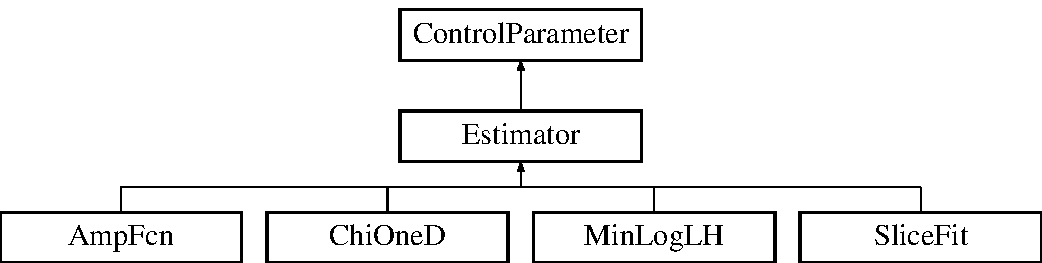
\includegraphics[height=3.000000cm]{class_estimator}
\end{center}
\end{figure}
\subsection*{Public Member Functions}
\begin{DoxyCompactItemize}
\item 
\hypertarget{class_estimator_a7546c738e4ec8709082390c7edbc0cb3}{virtual double {\bfseries control\-Parameter} (\hyperlink{class_parameter_list}{Parameter\-List} \&min\-Par)=0}\label{class_estimator_a7546c738e4ec8709082390c7edbc0cb3}

\end{DoxyCompactItemize}
\subsection*{Additional Inherited Members}


\subsection{Detailed Description}
\hyperlink{class_estimator}{Estimator} Interface Base-\/\-Class. 

The documentation for this class was generated from the following file\-:\begin{DoxyCompactItemize}
\item 
Estimator/\hyperlink{_estimator_8hpp}{Estimator.\-hpp}\end{DoxyCompactItemize}

\hypertarget{class_event}{\section{Event Class Reference}
\label{class_event}\index{Event@{Event}}
}


Internal container for event information.  




{\ttfamily \#include $<$Event.\-hpp$>$}

\subsection*{Public Member Functions}
\begin{DoxyCompactItemize}
\item 
\hypertarget{class_event_a9428d9a3c1019d5d0578361a1f1b5a21}{{\bfseries Event} (const double in\-Weight)}\label{class_event_a9428d9a3c1019d5d0578361a1f1b5a21}

\item 
\hypertarget{class_event_ac03f230c76575e2823d779fc99b0a310}{virtual void {\bfseries add\-Particle} (\hyperlink{struct_particle}{Particle} in\-Particle)}\label{class_event_ac03f230c76575e2823d779fc99b0a310}

\item 
\hypertarget{class_event_af6404986f4d6025c9f91db1964b7e964}{virtual const unsigned int {\bfseries get\-N\-Particles} ()}\label{class_event_af6404986f4d6025c9f91db1964b7e964}

\item 
\hypertarget{class_event_a1386cb0d462fdebdc54f2fdbda6c9004}{virtual const \hyperlink{struct_particle}{Particle} \& {\bfseries get\-Particle} (const unsigned int id)}\label{class_event_a1386cb0d462fdebdc54f2fdbda6c9004}

\end{DoxyCompactItemize}
\subsection*{Protected Attributes}
\begin{DoxyCompactItemize}
\item 
\hypertarget{class_event_a8b6abfa709a91c4109ab52237a364229}{std\-::vector$<$ \hyperlink{struct_particle}{Particle} $>$ {\bfseries f\-Particles}}\label{class_event_a8b6abfa709a91c4109ab52237a364229}

\item 
\hypertarget{class_event_af00af833e5d897490265fb19c8578485}{double {\bfseries f\-Weight}}\label{class_event_af00af833e5d897490265fb19c8578485}

\end{DoxyCompactItemize}


\subsection{Detailed Description}
Internal container for event information. 

The documentation for this class was generated from the following files\-:\begin{DoxyCompactItemize}
\item 
Core/\hyperlink{_event_8hpp}{Event.\-hpp}\item 
Core/Event.\-cpp\end{DoxyCompactItemize}

\hypertarget{class_exception}{\section{Exception Class Reference}
\label{class_exception}\index{Exception@{Exception}}
}


Com\-P\-W\-A Exceptions.  




{\ttfamily \#include $<$Exceptions.\-hpp$>$}

Inheritance diagram for Exception\-:\begin{figure}[H]
\begin{center}
\leavevmode
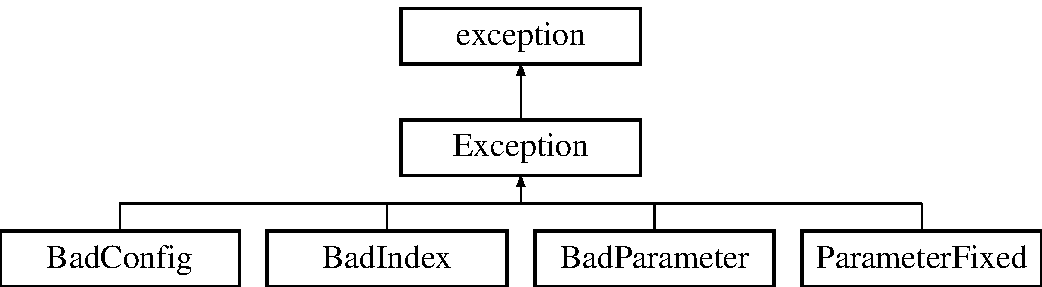
\includegraphics[height=3.000000cm]{class_exception}
\end{center}
\end{figure}
\subsection*{Public Member Functions}
\begin{DoxyCompactItemize}
\item 
\hypertarget{class_exception_adebf1b05f78135d58d634c7dc15590fc}{{\bfseries Exception} (const \hyperlink{class_exception}{Exception} \&e)  throw ()}\label{class_exception_adebf1b05f78135d58d634c7dc15590fc}

\item 
\hypertarget{class_exception_ad900a393018463dabfa6fcfb5c4d22ed}{\hyperlink{class_exception}{Exception} \& {\bfseries operator=} (const \hyperlink{class_exception}{Exception} \&rhs)  throw ()}\label{class_exception_ad900a393018463dabfa6fcfb5c4d22ed}

\item 
\hypertarget{class_exception_a78154a31544a609cbd226d32574f52cd}{virtual const char $\ast$ {\bfseries what} () const   throw ()}\label{class_exception_a78154a31544a609cbd226d32574f52cd}

\end{DoxyCompactItemize}
\subsection*{Protected Member Functions}
\begin{DoxyCompactItemize}
\item 
\hypertarget{class_exception_a158de64eeddf8fe336eeeb61f7cb8ef7}{{\bfseries Exception} (const char $\ast$w=\char`\"{}\char`\"{})  throw ()}\label{class_exception_a158de64eeddf8fe336eeeb61f7cb8ef7}

\item 
\hypertarget{class_exception_ae39c469513bf7efcede819d0086aa739}{{\bfseries Exception} (const std\-::string \&w)  throw ()}\label{class_exception_ae39c469513bf7efcede819d0086aa739}

\end{DoxyCompactItemize}
\subsection*{Protected Attributes}
\begin{DoxyCompactItemize}
\item 
\hypertarget{class_exception_a4dad5e3141a31867ef43fd3ccb5e147d}{std\-::string {\bfseries what\-\_\-}}\label{class_exception_a4dad5e3141a31867ef43fd3ccb5e147d}

\end{DoxyCompactItemize}


\subsection{Detailed Description}
Com\-P\-W\-A Exceptions. 

The documentation for this class was generated from the following file\-:\begin{DoxyCompactItemize}
\item 
Core/Exceptions.\-hpp\end{DoxyCompactItemize}

\hypertarget{class_geneva_i_f}{\section{Geneva\-I\-F Class Reference}
\label{class_geneva_i_f}\index{Geneva\-I\-F@{Geneva\-I\-F}}
}


Wrapper of the Geneva \hyperlink{class_optimizer}{Optimizer} library.  




{\ttfamily \#include $<$Geneva\-I\-F.\-hpp$>$}

Inheritance diagram for Geneva\-I\-F\-:\begin{figure}[H]
\begin{center}
\leavevmode
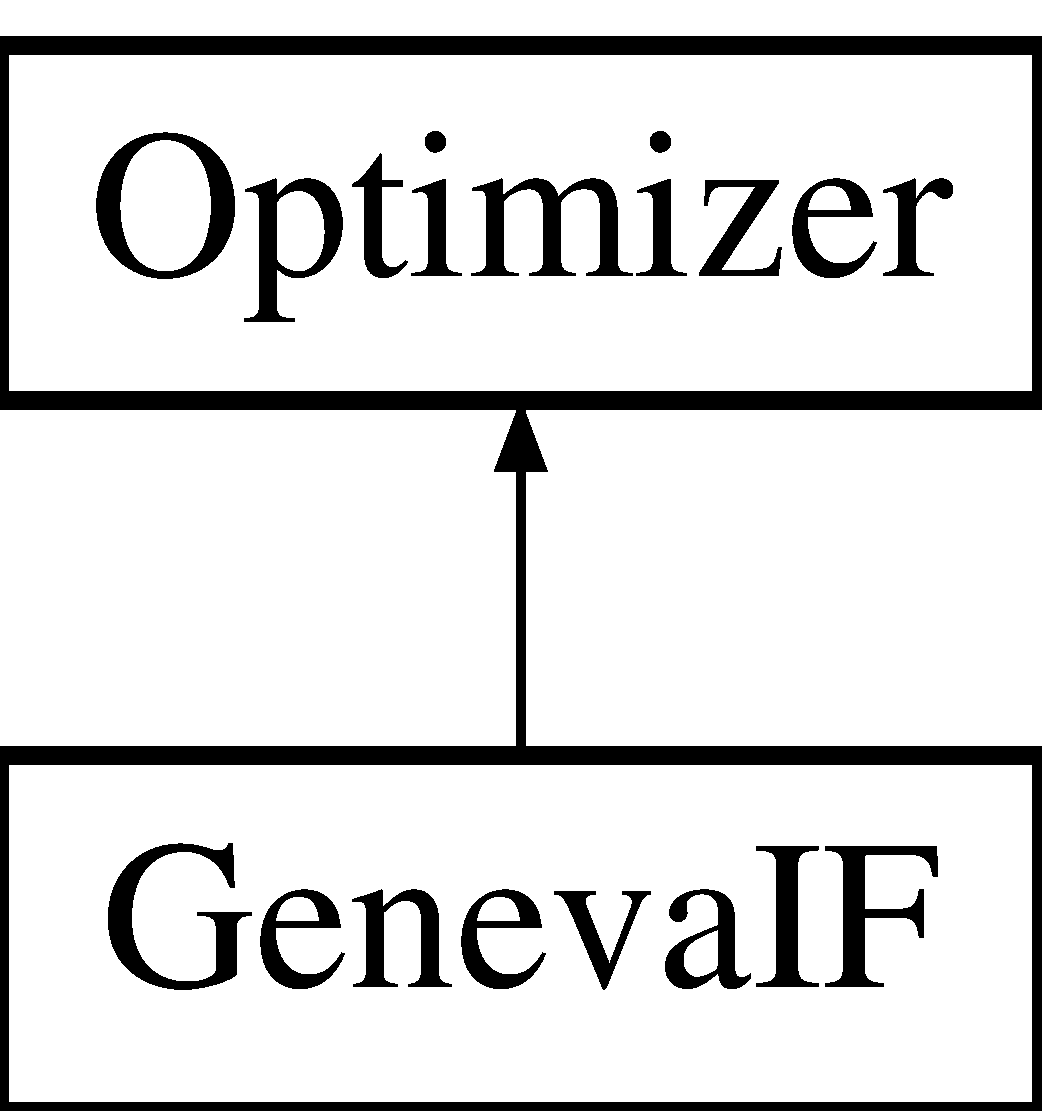
\includegraphics[height=2.000000cm]{class_geneva_i_f}
\end{center}
\end{figure}
\subsection*{Public Member Functions}
\begin{DoxyCompactItemize}
\item 
\hypertarget{class_geneva_i_f_a2ab9fc95b61a5f21856245ca9de7c51d}{\hyperlink{class_geneva_i_f_a2ab9fc95b61a5f21856245ca9de7c51d}{Geneva\-I\-F} (std\-::shared\-\_\-ptr$<$ \hyperlink{class_control_parameter}{Control\-Parameter} $>$ the\-Data, std\-::string in\-Config\-File\-Dir=\char`\"{}test/config/\char`\"{})}\label{class_geneva_i_f_a2ab9fc95b61a5f21856245ca9de7c51d}

\begin{DoxyCompactList}\small\item\em Default Constructor (0x0) \end{DoxyCompactList}\item 
\hypertarget{class_geneva_i_f_a2f4ed9d5cf44575da316c6f52e863315}{virtual const double {\bfseries exec} (\hyperlink{class_parameter_list}{Parameter\-List} \&par)}\label{class_geneva_i_f_a2f4ed9d5cf44575da316c6f52e863315}

\item 
virtual \hyperlink{class_geneva_i_f_ac1dcb675cdeceae9335157f1c2560fe9}{$\sim$\-Geneva\-I\-F} ()
\item 
\hypertarget{class_geneva_i_f_a5c98aa241df27f176203d5f585b1c47c}{virtual void {\bfseries set\-Server\-Mode} ()}\label{class_geneva_i_f_a5c98aa241df27f176203d5f585b1c47c}

\item 
\hypertarget{class_geneva_i_f_ab23559f5d3482d0e281f1ecf0848b5bb}{virtual void {\bfseries set\-Client\-Mode} (std\-::string serverip=\char`\"{}localhost\char`\"{}, unsigned int serverport=10000)}\label{class_geneva_i_f_ab23559f5d3482d0e281f1ecf0848b5bb}

\end{DoxyCompactItemize}


\subsection{Detailed Description}
Wrapper of the Geneva \hyperlink{class_optimizer}{Optimizer} library. 

\subsection{Constructor \& Destructor Documentation}
\hypertarget{class_geneva_i_f_ac1dcb675cdeceae9335157f1c2560fe9}{\index{Geneva\-I\-F@{Geneva\-I\-F}!$\sim$\-Geneva\-I\-F@{$\sim$\-Geneva\-I\-F}}
\index{$\sim$\-Geneva\-I\-F@{$\sim$\-Geneva\-I\-F}!GenevaIF@{Geneva\-I\-F}}
\subsubsection[{$\sim$\-Geneva\-I\-F}]{\setlength{\rightskip}{0pt plus 5cm}Geneva\-I\-F\-::$\sim$\-Geneva\-I\-F (
\begin{DoxyParamCaption}
{}
\end{DoxyParamCaption}
)\hspace{0.3cm}{\ttfamily [virtual]}}}\label{class_geneva_i_f_ac1dcb675cdeceae9335157f1c2560fe9}
Destructor 

The documentation for this class was generated from the following files\-:\begin{DoxyCompactItemize}
\item 
Optimizer/\-Geneva/\hyperlink{_geneva_i_f_8hpp}{Geneva\-I\-F.\-hpp}\item 
Optimizer/\-Geneva/Geneva\-I\-F.\-cpp\end{DoxyCompactItemize}

\hypertarget{class_gem_1_1_geneva_1_1_g_start_individual}{\section{Gem\-:\-:Geneva\-:\-:G\-Start\-Individual Class Reference}
\label{class_gem_1_1_geneva_1_1_g_start_individual}\index{Gem\-::\-Geneva\-::\-G\-Start\-Individual@{Gem\-::\-Geneva\-::\-G\-Start\-Individual}}
}


{\ttfamily \#include $<$G\-Start\-Individual.\-hpp$>$}

Inheritance diagram for Gem\-:\-:Geneva\-:\-:G\-Start\-Individual\-:\begin{figure}[H]
\begin{center}
\leavevmode
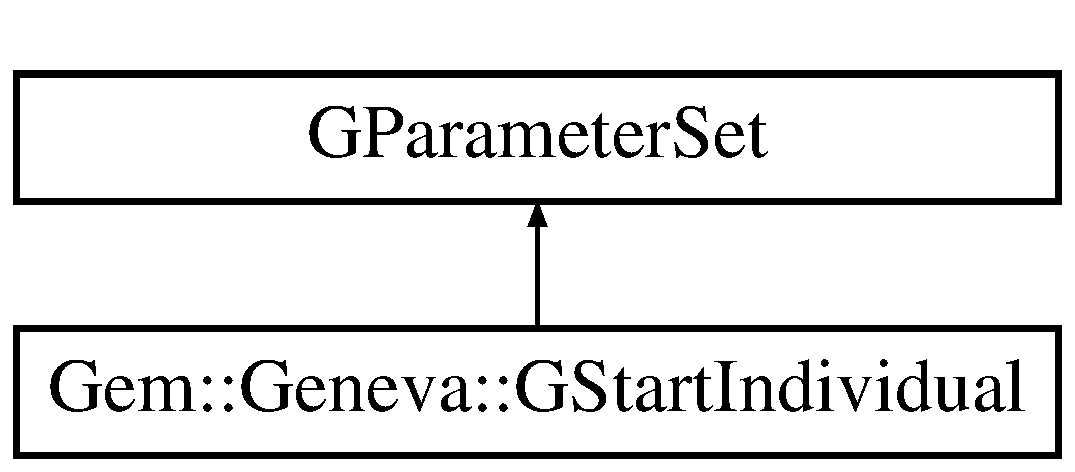
\includegraphics[height=2.000000cm]{class_gem_1_1_geneva_1_1_g_start_individual}
\end{center}
\end{figure}
\subsection*{Public Member Functions}
\begin{DoxyCompactItemize}
\item 
\hyperlink{class_gem_1_1_geneva_1_1_g_start_individual_a9e281091f2371b021c94af6c9b9ef5fa}{G\-Start\-Individual} (std\-::shared\-\_\-ptr$<$ \hyperlink{class_control_parameter}{Control\-Parameter} $>$ data, unsigned int par\-Dim, double $\ast$val, double $\ast$min, double $\ast$max, double $\ast$err)
\begin{DoxyCompactList}\small\item\em The default constructor. \end{DoxyCompactList}\item 
\hyperlink{class_gem_1_1_geneva_1_1_g_start_individual_a185646ccd2416e89a83c45de79388e60}{G\-Start\-Individual} (const \hyperlink{class_gem_1_1_geneva_1_1_g_start_individual}{G\-Start\-Individual} \&)
\begin{DoxyCompactList}\small\item\em A standard copy constructor. \end{DoxyCompactList}\item 
virtual \hyperlink{class_gem_1_1_geneva_1_1_g_start_individual_aad3e6125efd6fcb7066d1142cc2807aa}{$\sim$\-G\-Start\-Individual} ()
\begin{DoxyCompactList}\small\item\em The standard destructor. \end{DoxyCompactList}\item 
bool \hyperlink{class_gem_1_1_geneva_1_1_g_start_individual_a755a7425d632903b27d398d1432a0a16}{get\-Par} (\hyperlink{class_parameter_list}{Parameter\-List} \&val)
\item 
const \hyperlink{class_gem_1_1_geneva_1_1_g_start_individual}{G\-Start\-Individual} \& \hyperlink{class_gem_1_1_geneva_1_1_g_start_individual_a8fcd717bd9468901eb78b90ca02438ed}{operator=} (const \hyperlink{class_gem_1_1_geneva_1_1_g_start_individual}{G\-Start\-Individual} \&)
\begin{DoxyCompactList}\small\item\em A standard assignment operator. \end{DoxyCompactList}\end{DoxyCompactItemize}
\subsection*{Protected Member Functions}
\begin{DoxyCompactItemize}
\item 
virtual void \hyperlink{class_gem_1_1_geneva_1_1_g_start_individual_a012447d3b9772d94b8d4d35fb4fc2304}{load\-\_\-} (const G\-Object $\ast$)
\begin{DoxyCompactList}\small\item\em Loads the data of another \hyperlink{class_gem_1_1_geneva_1_1_g_start_individual}{G\-Start\-Individual}. \end{DoxyCompactList}\item 
virtual G\-Object $\ast$ \hyperlink{class_gem_1_1_geneva_1_1_g_start_individual_aa7d75cb7a4b93a2d766d99bdc11ebb73}{clone\-\_\-} () const 
\begin{DoxyCompactList}\small\item\em Creates a deep clone of this object. \end{DoxyCompactList}\item 
virtual void \hyperlink{class_gem_1_1_geneva_1_1_g_start_individual_a639b1102996bc7d57b872b69f53f5726}{load\-Constant\-Data} (boost\-::shared\-\_\-ptr$<$ Gem\-::\-Geneva\-::\-G\-Individual $>$)
\begin{DoxyCompactList}\small\item\em Loads static data. \end{DoxyCompactList}\item 
virtual double \hyperlink{class_gem_1_1_geneva_1_1_g_start_individual_a98d31a7196d550fc9ce0166f7041ca2b}{fitness\-Calculation} ()
\begin{DoxyCompactList}\small\item\em The actual fitness calculation takes place here. \end{DoxyCompactList}\end{DoxyCompactItemize}
\subsection*{Friends}
\begin{DoxyCompactItemize}
\item 
\hypertarget{class_gem_1_1_geneva_1_1_g_start_individual_ac98d07dd8f7b70e16ccb9a01abf56b9c}{class \hyperlink{class_gem_1_1_geneva_1_1_g_start_individual_ac98d07dd8f7b70e16ccb9a01abf56b9c}{boost\-::serialization\-::access}}\label{class_gem_1_1_geneva_1_1_g_start_individual_ac98d07dd8f7b70e16ccb9a01abf56b9c}

\begin{DoxyCompactList}\small\item\em Make the class accessible to Boost.\-Serialization. \end{DoxyCompactList}\end{DoxyCompactItemize}


\subsection{Detailed Description}
This individual searches for the minimum of a 2-\/dimensional parabola. It is part of an introductory example, used in the Geneva manual. 

\subsection{Constructor \& Destructor Documentation}
\hypertarget{class_gem_1_1_geneva_1_1_g_start_individual_a9e281091f2371b021c94af6c9b9ef5fa}{\index{Gem\-::\-Geneva\-::\-G\-Start\-Individual@{Gem\-::\-Geneva\-::\-G\-Start\-Individual}!G\-Start\-Individual@{G\-Start\-Individual}}
\index{G\-Start\-Individual@{G\-Start\-Individual}!Gem::Geneva::GStartIndividual@{Gem\-::\-Geneva\-::\-G\-Start\-Individual}}
\subsubsection[{G\-Start\-Individual}]{\setlength{\rightskip}{0pt plus 5cm}Gem\-::\-Geneva\-::\-G\-Start\-Individual\-::\-G\-Start\-Individual (
\begin{DoxyParamCaption}
\item[{std\-::shared\-\_\-ptr$<$ {\bf Control\-Parameter} $>$}]{data, }
\item[{unsigned int}]{par\-Dim, }
\item[{double $\ast$}]{val, }
\item[{double $\ast$}]{min, }
\item[{double $\ast$}]{max, }
\item[{double $\ast$}]{err}
\end{DoxyParamCaption}
)}}\label{class_gem_1_1_geneva_1_1_g_start_individual_a9e281091f2371b021c94af6c9b9ef5fa}


The default constructor. 

The default constructor. This function will add two double parameters to this individual, each of which has a constrained value range \mbox{[}-\/10\-:10\mbox{]}. \hypertarget{class_gem_1_1_geneva_1_1_g_start_individual_a185646ccd2416e89a83c45de79388e60}{\index{Gem\-::\-Geneva\-::\-G\-Start\-Individual@{Gem\-::\-Geneva\-::\-G\-Start\-Individual}!G\-Start\-Individual@{G\-Start\-Individual}}
\index{G\-Start\-Individual@{G\-Start\-Individual}!Gem::Geneva::GStartIndividual@{Gem\-::\-Geneva\-::\-G\-Start\-Individual}}
\subsubsection[{G\-Start\-Individual}]{\setlength{\rightskip}{0pt plus 5cm}Gem\-::\-Geneva\-::\-G\-Start\-Individual\-::\-G\-Start\-Individual (
\begin{DoxyParamCaption}
\item[{const {\bf G\-Start\-Individual} \&}]{cp}
\end{DoxyParamCaption}
)}}\label{class_gem_1_1_geneva_1_1_g_start_individual_a185646ccd2416e89a83c45de79388e60}


A standard copy constructor. 

A standard copy constructor. All real work is done by the parent class.


\begin{DoxyParams}{Parameters}
{\em cp} & A copy of another \hyperlink{class_gem_1_1_geneva_1_1_g_start_individual}{G\-Start\-Individual} \\
\hline
\end{DoxyParams}
\hypertarget{class_gem_1_1_geneva_1_1_g_start_individual_aad3e6125efd6fcb7066d1142cc2807aa}{\index{Gem\-::\-Geneva\-::\-G\-Start\-Individual@{Gem\-::\-Geneva\-::\-G\-Start\-Individual}!$\sim$\-G\-Start\-Individual@{$\sim$\-G\-Start\-Individual}}
\index{$\sim$\-G\-Start\-Individual@{$\sim$\-G\-Start\-Individual}!Gem::Geneva::GStartIndividual@{Gem\-::\-Geneva\-::\-G\-Start\-Individual}}
\subsubsection[{$\sim$\-G\-Start\-Individual}]{\setlength{\rightskip}{0pt plus 5cm}Gem\-::\-Geneva\-::\-G\-Start\-Individual\-::$\sim$\-G\-Start\-Individual (
\begin{DoxyParamCaption}
{}
\end{DoxyParamCaption}
)\hspace{0.3cm}{\ttfamily [virtual]}}}\label{class_gem_1_1_geneva_1_1_g_start_individual_aad3e6125efd6fcb7066d1142cc2807aa}


The standard destructor. 

The standard destructor. Note that you do not need to care for the parameter objects added in the constructor. Upon destruction, they will take care of releasing the allocated memory. 

\subsection{Member Function Documentation}
\hypertarget{class_gem_1_1_geneva_1_1_g_start_individual_aa7d75cb7a4b93a2d766d99bdc11ebb73}{\index{Gem\-::\-Geneva\-::\-G\-Start\-Individual@{Gem\-::\-Geneva\-::\-G\-Start\-Individual}!clone\-\_\-@{clone\-\_\-}}
\index{clone\-\_\-@{clone\-\_\-}!Gem::Geneva::GStartIndividual@{Gem\-::\-Geneva\-::\-G\-Start\-Individual}}
\subsubsection[{clone\-\_\-}]{\setlength{\rightskip}{0pt plus 5cm}G\-Object $\ast$ Gem\-::\-Geneva\-::\-G\-Start\-Individual\-::clone\-\_\- (
\begin{DoxyParamCaption}
{}
\end{DoxyParamCaption}
) const\hspace{0.3cm}{\ttfamily [protected]}, {\ttfamily [virtual]}}}\label{class_gem_1_1_geneva_1_1_g_start_individual_aa7d75cb7a4b93a2d766d99bdc11ebb73}


Creates a deep clone of this object. 

Creates a deep clone of this object

\begin{DoxyReturn}{Returns}
A deep clone of this object, camouflaged as a G\-Object 
\end{DoxyReturn}
\hypertarget{class_gem_1_1_geneva_1_1_g_start_individual_a98d31a7196d550fc9ce0166f7041ca2b}{\index{Gem\-::\-Geneva\-::\-G\-Start\-Individual@{Gem\-::\-Geneva\-::\-G\-Start\-Individual}!fitness\-Calculation@{fitness\-Calculation}}
\index{fitness\-Calculation@{fitness\-Calculation}!Gem::Geneva::GStartIndividual@{Gem\-::\-Geneva\-::\-G\-Start\-Individual}}
\subsubsection[{fitness\-Calculation}]{\setlength{\rightskip}{0pt plus 5cm}double Gem\-::\-Geneva\-::\-G\-Start\-Individual\-::fitness\-Calculation (
\begin{DoxyParamCaption}
{}
\end{DoxyParamCaption}
)\hspace{0.3cm}{\ttfamily [protected]}, {\ttfamily [virtual]}}}\label{class_gem_1_1_geneva_1_1_g_start_individual_a98d31a7196d550fc9ce0166f7041ca2b}


The actual fitness calculation takes place here. 

The actual fitness calculation takes place here.

\begin{DoxyReturn}{Returns}
The value of this object 
\end{DoxyReturn}
\hypertarget{class_gem_1_1_geneva_1_1_g_start_individual_a755a7425d632903b27d398d1432a0a16}{\index{Gem\-::\-Geneva\-::\-G\-Start\-Individual@{Gem\-::\-Geneva\-::\-G\-Start\-Individual}!get\-Par@{get\-Par}}
\index{get\-Par@{get\-Par}!Gem::Geneva::GStartIndividual@{Gem\-::\-Geneva\-::\-G\-Start\-Individual}}
\subsubsection[{get\-Par}]{\setlength{\rightskip}{0pt plus 5cm}bool Gem\-::\-Geneva\-::\-G\-Start\-Individual\-::get\-Par (
\begin{DoxyParamCaption}
\item[{{\bf Parameter\-List} \&}]{val}
\end{DoxyParamCaption}
)}}\label{class_gem_1_1_geneva_1_1_g_start_individual_a755a7425d632903b27d398d1432a0a16}
Access the Parameter


\begin{DoxyParams}{Parameters}
{\em val} & The \hyperlink{class_parameter_list}{Parameter\-List} to fill \\
\hline
\end{DoxyParams}
\begin{DoxyReturn}{Returns}
bool if valid 
\end{DoxyReturn}
\hypertarget{class_gem_1_1_geneva_1_1_g_start_individual_a012447d3b9772d94b8d4d35fb4fc2304}{\index{Gem\-::\-Geneva\-::\-G\-Start\-Individual@{Gem\-::\-Geneva\-::\-G\-Start\-Individual}!load\-\_\-@{load\-\_\-}}
\index{load\-\_\-@{load\-\_\-}!Gem::Geneva::GStartIndividual@{Gem\-::\-Geneva\-::\-G\-Start\-Individual}}
\subsubsection[{load\-\_\-}]{\setlength{\rightskip}{0pt plus 5cm}void Gem\-::\-Geneva\-::\-G\-Start\-Individual\-::load\-\_\- (
\begin{DoxyParamCaption}
\item[{const G\-Object $\ast$}]{cp}
\end{DoxyParamCaption}
)\hspace{0.3cm}{\ttfamily [protected]}, {\ttfamily [virtual]}}}\label{class_gem_1_1_geneva_1_1_g_start_individual_a012447d3b9772d94b8d4d35fb4fc2304}


Loads the data of another \hyperlink{class_gem_1_1_geneva_1_1_g_start_individual}{G\-Start\-Individual}. 

Loads the data of another \hyperlink{class_gem_1_1_geneva_1_1_g_start_individual}{G\-Start\-Individual}, camouflaged as a G\-Object.


\begin{DoxyParams}{Parameters}
{\em cp} & A copy of another \hyperlink{class_gem_1_1_geneva_1_1_g_start_individual}{G\-Start\-Individual}, camouflaged as a G\-Object \\
\hline
\end{DoxyParams}
\hypertarget{class_gem_1_1_geneva_1_1_g_start_individual_a639b1102996bc7d57b872b69f53f5726}{\index{Gem\-::\-Geneva\-::\-G\-Start\-Individual@{Gem\-::\-Geneva\-::\-G\-Start\-Individual}!load\-Constant\-Data@{load\-Constant\-Data}}
\index{load\-Constant\-Data@{load\-Constant\-Data}!Gem::Geneva::GStartIndividual@{Gem\-::\-Geneva\-::\-G\-Start\-Individual}}
\subsubsection[{load\-Constant\-Data}]{\setlength{\rightskip}{0pt plus 5cm}void Gem\-::\-Geneva\-::\-G\-Start\-Individual\-::load\-Constant\-Data (
\begin{DoxyParamCaption}
\item[{boost\-::shared\-\_\-ptr$<$ Gem\-::\-Geneva\-::\-G\-Individual $>$}]{}
\end{DoxyParamCaption}
)\hspace{0.3cm}{\ttfamily [protected]}, {\ttfamily [virtual]}}}\label{class_gem_1_1_geneva_1_1_g_start_individual_a639b1102996bc7d57b872b69f53f5726}


Loads static data. 

Loads all static data needed in client mode. \hypertarget{class_gem_1_1_geneva_1_1_g_start_individual_a8fcd717bd9468901eb78b90ca02438ed}{\index{Gem\-::\-Geneva\-::\-G\-Start\-Individual@{Gem\-::\-Geneva\-::\-G\-Start\-Individual}!operator=@{operator=}}
\index{operator=@{operator=}!Gem::Geneva::GStartIndividual@{Gem\-::\-Geneva\-::\-G\-Start\-Individual}}
\subsubsection[{operator=}]{\setlength{\rightskip}{0pt plus 5cm}const {\bf G\-Start\-Individual} \& Gem\-::\-Geneva\-::\-G\-Start\-Individual\-::operator= (
\begin{DoxyParamCaption}
\item[{const {\bf G\-Start\-Individual} \&}]{cp}
\end{DoxyParamCaption}
)}}\label{class_gem_1_1_geneva_1_1_g_start_individual_a8fcd717bd9468901eb78b90ca02438ed}


A standard assignment operator. 

A standard assignment operator


\begin{DoxyParams}{Parameters}
{\em cp} & A copy of another \hyperlink{class_gem_1_1_geneva_1_1_g_start_individual}{G\-Start\-Individual} object \\
\hline
\end{DoxyParams}
\begin{DoxyReturn}{Returns}
A constant reference to this object 
\end{DoxyReturn}


The documentation for this class was generated from the following files\-:\begin{DoxyCompactItemize}
\item 
Optimizer/\-Geneva/\hyperlink{_g_start_individual_8hpp}{G\-Start\-Individual.\-hpp}\item 
Optimizer/\-Geneva/G\-Start\-Individual.\-cpp\end{DoxyCompactItemize}

\hypertarget{class_integer_parameter}{\section{Integer\-Parameter Class Reference}
\label{class_integer_parameter}\index{Integer\-Parameter@{Integer\-Parameter}}
}
\subsection*{Public Member Functions}
\begin{DoxyCompactItemize}
\item 
\hyperlink{class_integer_parameter_a3b6c7d2cf7e6e405618c28477c4a6163}{Integer\-Parameter} ()
\begin{DoxyCompactList}\small\item\em Standard constructor without information. \end{DoxyCompactList}\item 
\hyperlink{class_integer_parameter_a342142d0c742fa3beb1c691cd2d6c4ad}{Integer\-Parameter} (const int value)
\begin{DoxyCompactList}\small\item\em Standard constructor with a value. \end{DoxyCompactList}\item 
\hyperlink{class_integer_parameter_aa9d240d2ba83905ffa1cfd9fe1b1c213}{Integer\-Parameter} (const int value, const int error)
\begin{DoxyCompactList}\small\item\em Standard constructor with value and error. \end{DoxyCompactList}\item 
\hyperlink{class_integer_parameter_ab71291d38ec332a26558ee01fae1985c}{Integer\-Parameter} (const int value, const int min, const int max)
\begin{DoxyCompactList}\small\item\em Standard constructor with value and bounds. \end{DoxyCompactList}\item 
\hyperlink{class_integer_parameter_a79d506e1eaaba1fd38d2b450d7c19667}{Integer\-Parameter} (const int value, const int min, const int max, const int error)
\begin{DoxyCompactList}\small\item\em Standard constructor with value, bounds and error. \end{DoxyCompactList}\item 
\hyperlink{class_integer_parameter_a4601b4b1d68bac1e0a599324e3c5b1fb}{Integer\-Parameter} (const \hyperlink{class_integer_parameter}{Integer\-Parameter} \&in)
\begin{DoxyCompactList}\small\item\em Copy constructor using = operator. \end{DoxyCompactList}\item 
virtual \hyperlink{class_integer_parameter_a66cbb6a345278f86c5af0fdb2961aa95}{$\sim$\-Integer\-Parameter} ()
\begin{DoxyCompactList}\small\item\em Empty Destructor. \end{DoxyCompactList}\item 
\hypertarget{class_integer_parameter_a321225fbd82f3d272af0b0785c293014}{virtual const bool \hyperlink{class_integer_parameter_a321225fbd82f3d272af0b0785c293014}{Has\-Bounds} () const }\label{class_integer_parameter_a321225fbd82f3d272af0b0785c293014}

\begin{DoxyCompactList}\small\item\em Check if parameter has bounds. \end{DoxyCompactList}\item 
\hypertarget{class_integer_parameter_a2fa6e3a0cb1c288b8dd3d37860b6dea1}{virtual const bool \hyperlink{class_integer_parameter_a2fa6e3a0cb1c288b8dd3d37860b6dea1}{Use\-Bounds} () const }\label{class_integer_parameter_a2fa6e3a0cb1c288b8dd3d37860b6dea1}

\begin{DoxyCompactList}\small\item\em Check if bounds should be used. \end{DoxyCompactList}\item 
\hypertarget{class_integer_parameter_abbd590feb425e997ff3bd635c2708ef8}{virtual const bool \hyperlink{class_integer_parameter_abbd590feb425e997ff3bd635c2708ef8}{Has\-Error} () const }\label{class_integer_parameter_abbd590feb425e997ff3bd635c2708ef8}

\begin{DoxyCompactList}\small\item\em Check if parameter has an error. \end{DoxyCompactList}\item 
\hypertarget{class_integer_parameter_ae5779fb4971fce0b087b2b601ba1d6ea}{virtual const bool \hyperlink{class_integer_parameter_ae5779fb4971fce0b087b2b601ba1d6ea}{Is\-Fixed} () const }\label{class_integer_parameter_ae5779fb4971fce0b087b2b601ba1d6ea}

\begin{DoxyCompactList}\small\item\em Check if parameter is fixed. \end{DoxyCompactList}\item 
\hypertarget{class_integer_parameter_a26592ec6fde9f8991306037826be90ca}{virtual const int \hyperlink{class_integer_parameter_a26592ec6fde9f8991306037826be90ca}{Get\-Value} () const }\label{class_integer_parameter_a26592ec6fde9f8991306037826be90ca}

\begin{DoxyCompactList}\small\item\em Getter for value of parameter. \end{DoxyCompactList}\item 
\hypertarget{class_integer_parameter_a266385f52f2c760732c25adcc1419e8b}{virtual const int \hyperlink{class_integer_parameter_a266385f52f2c760732c25adcc1419e8b}{Get\-Min\-Value} () const }\label{class_integer_parameter_a266385f52f2c760732c25adcc1419e8b}

\begin{DoxyCompactList}\small\item\em Getter for lower bound of parameter. \end{DoxyCompactList}\item 
\hypertarget{class_integer_parameter_ab70d708a642c3b78b8f72991e140c77c}{virtual const int \hyperlink{class_integer_parameter_ab70d708a642c3b78b8f72991e140c77c}{Get\-Max\-Value} () const }\label{class_integer_parameter_ab70d708a642c3b78b8f72991e140c77c}

\begin{DoxyCompactList}\small\item\em Getter for upper bound of parameter. \end{DoxyCompactList}\item 
\hypertarget{class_integer_parameter_a544118e88bfe32f43606adeee1ff9985}{virtual const int \hyperlink{class_integer_parameter_a544118e88bfe32f43606adeee1ff9985}{Get\-Error} () const }\label{class_integer_parameter_a544118e88bfe32f43606adeee1ff9985}

\begin{DoxyCompactList}\small\item\em Getter for error of parameter. \end{DoxyCompactList}\item 
\hypertarget{class_integer_parameter_a681cf09d9d150835450446cd7b8b2cfb}{virtual void \hyperlink{class_integer_parameter_a681cf09d9d150835450446cd7b8b2cfb}{Set\-Value} (const int in\-Val)}\label{class_integer_parameter_a681cf09d9d150835450446cd7b8b2cfb}

\begin{DoxyCompactList}\small\item\em Setter for value of parameter. \end{DoxyCompactList}\item 
\hypertarget{class_integer_parameter_a91d73f38cbbf3a344a9355c459a34145}{virtual void \hyperlink{class_integer_parameter_a91d73f38cbbf3a344a9355c459a34145}{Set\-Error} (const int in\-Err)}\label{class_integer_parameter_a91d73f38cbbf3a344a9355c459a34145}

\begin{DoxyCompactList}\small\item\em Setter for error of parameter. \end{DoxyCompactList}\item 
\hypertarget{class_integer_parameter_ace6b35a334076dafd65124709c096098}{virtual const bool \hyperlink{class_integer_parameter_ace6b35a334076dafd65124709c096098}{Set\-Min\-Max} (const int in\-Min, const int in\-Max)}\label{class_integer_parameter_ace6b35a334076dafd65124709c096098}

\begin{DoxyCompactList}\small\item\em Setter for bounds of parameter. \end{DoxyCompactList}\item 
virtual const bool \hyperlink{class_integer_parameter_a8a9aa6481a17e2f9c81c72c758050b95}{Set\-Min\-Value} (const int min)
\begin{DoxyCompactList}\small\item\em Setter for lower bound. \end{DoxyCompactList}\item 
virtual const bool \hyperlink{class_integer_parameter_a25e9abebc74581a887aadbd6c60e431f}{Set\-Max\-Value} (const int max)
\begin{DoxyCompactList}\small\item\em Setter for upper bound. \end{DoxyCompactList}\item 
\hypertarget{class_integer_parameter_aed709aa9573ad1ebd0e6bdd0923847cc}{virtual const void \hyperlink{class_integer_parameter_aed709aa9573ad1ebd0e6bdd0923847cc}{Use\-Bounds} (const bool use)}\label{class_integer_parameter_aed709aa9573ad1ebd0e6bdd0923847cc}

\begin{DoxyCompactList}\small\item\em Set if bounds should be used. \end{DoxyCompactList}\item 
\hypertarget{class_integer_parameter_a0b2857e6e04aa72260601eb1d8d04822}{virtual const void \hyperlink{class_integer_parameter_a0b2857e6e04aa72260601eb1d8d04822}{Set\-Parameter\-Fixed} ()}\label{class_integer_parameter_a0b2857e6e04aa72260601eb1d8d04822}

\begin{DoxyCompactList}\small\item\em Call to fix parameter. \end{DoxyCompactList}\item 
\hypertarget{class_integer_parameter_aaf5d8de1cad5e36a8390a4f1c6a1e4e1}{virtual const void \hyperlink{class_integer_parameter_aaf5d8de1cad5e36a8390a4f1c6a1e4e1}{Set\-Parameter\-Free} ()}\label{class_integer_parameter_aaf5d8de1cad5e36a8390a4f1c6a1e4e1}

\begin{DoxyCompactList}\small\item\em Call to free parameter. \end{DoxyCompactList}\item 
\hypertarget{class_integer_parameter_addaf4594889140804622055648cb4205}{virtual const void \hyperlink{class_integer_parameter_addaf4594889140804622055648cb4205}{Fix\-Parameter} (const bool fixed)}\label{class_integer_parameter_addaf4594889140804622055648cb4205}

\begin{DoxyCompactList}\small\item\em Set parameter free or fixed. \end{DoxyCompactList}\item 
std\-::string const \& \hyperlink{class_integer_parameter_a6e4a624ea0599cffcfc5f420b7931a36}{to\-\_\-str} () const 
\begin{DoxyCompactList}\small\item\em A public function returning a string with parameter information. \end{DoxyCompactList}\item 
virtual const std\-::string \hyperlink{class_integer_parameter_ae1452a0f19fa7c5140b12f39c6fd1300}{type} ()
\begin{DoxyCompactList}\small\item\em A public function returning a string naming its type. \end{DoxyCompactList}\item 
\hypertarget{class_integer_parameter_a4d4097e57daf46dfb5131ede39acc578}{{\bfseries operator int} () const }\label{class_integer_parameter_a4d4097e57daf46dfb5131ede39acc578}

\end{DoxyCompactItemize}
\subsection*{Protected Member Functions}
\begin{DoxyCompactItemize}
\item 
bool \hyperlink{class_integer_parameter_a0d33cf98f71bd2c2e3106989398a271b}{check\-\_\-bounds} (const int min, const int max)
\begin{DoxyCompactList}\small\item\em A protected function to check if bounds are valid. \end{DoxyCompactList}\item 
virtual void \hyperlink{class_integer_parameter_a0432071f33c3d53b730dbe888ff90f46}{make\-\_\-str} ()
\begin{DoxyCompactList}\small\item\em A protected function which creates an output string for printing. \end{DoxyCompactList}\end{DoxyCompactItemize}
\subsection*{Protected Attributes}
\begin{DoxyCompactItemize}
\item 
std\-::string \hyperlink{class_integer_parameter_abf6356e2879d6f09f45a52d65844998f}{out\-\_\-}
\item 
bool \hyperlink{class_integer_parameter_a6f95c4b841a3d669d15c46e787f73153}{bounds\-\_\-}
\item 
bool \hyperlink{class_integer_parameter_a611862af84b9db773cf8690fb0f888fb}{error\-\_\-}
\item 
bool \hyperlink{class_integer_parameter_ab68632ed3d270b082ebfb16de643e3df}{usebounds\-\_\-}
\item 
bool \hyperlink{class_integer_parameter_a7a3f5d9413ccb5fd1814a7db9e77dcfc}{fixed\-\_\-}
\item 
\hypertarget{class_integer_parameter_a2e91e7ac1f8e3881928738e0354bffea}{int {\bfseries val\-\_\-}}\label{class_integer_parameter_a2e91e7ac1f8e3881928738e0354bffea}

\item 
\hypertarget{class_integer_parameter_a7d37150cc66baebfd0a7cb0679dd8705}{int {\bfseries min\-\_\-}}\label{class_integer_parameter_a7d37150cc66baebfd0a7cb0679dd8705}

\item 
\hypertarget{class_integer_parameter_af4d3eab97deb4577e316d210e51ebd7c}{int {\bfseries max\-\_\-}}\label{class_integer_parameter_af4d3eab97deb4577e316d210e51ebd7c}

\item 
int \hyperlink{class_integer_parameter_a713ac37a8c8d820e212881178719ae91}{err\-\_\-}
\end{DoxyCompactItemize}
\subsection*{Friends}
\begin{DoxyCompactItemize}
\item 
std\-::ostream \& \hyperlink{class_integer_parameter_ab9a320e078948aa0ce31b2adec766bfc}{operator$<$$<$} (std\-::ostream \&os, const \hyperlink{class_integer_parameter}{Integer\-Parameter} \&p)
\begin{DoxyCompactList}\small\item\em friend function to stream parameter information to output \end{DoxyCompactList}\end{DoxyCompactItemize}


\subsection{Constructor \& Destructor Documentation}
\hypertarget{class_integer_parameter_a3b6c7d2cf7e6e405618c28477c4a6163}{\index{Integer\-Parameter@{Integer\-Parameter}!Integer\-Parameter@{Integer\-Parameter}}
\index{Integer\-Parameter@{Integer\-Parameter}!IntegerParameter@{Integer\-Parameter}}
\subsubsection[{Integer\-Parameter}]{\setlength{\rightskip}{0pt plus 5cm}Integer\-Parameter\-::\-Integer\-Parameter (
\begin{DoxyParamCaption}
{}
\end{DoxyParamCaption}
)\hspace{0.3cm}{\ttfamily [inline]}}}\label{class_integer_parameter_a3b6c7d2cf7e6e405618c28477c4a6163}


Standard constructor without information. 

Standard constructor with no information provided. Creates parameter with value 0 but without bounds or an error. \begin{DoxySeeAlso}{See Also}
\hyperlink{class_integer_parameter_a0432071f33c3d53b730dbe888ff90f46}{make\-\_\-str()} 
\end{DoxySeeAlso}
\hypertarget{class_integer_parameter_a342142d0c742fa3beb1c691cd2d6c4ad}{\index{Integer\-Parameter@{Integer\-Parameter}!Integer\-Parameter@{Integer\-Parameter}}
\index{Integer\-Parameter@{Integer\-Parameter}!IntegerParameter@{Integer\-Parameter}}
\subsubsection[{Integer\-Parameter}]{\setlength{\rightskip}{0pt plus 5cm}Integer\-Parameter\-::\-Integer\-Parameter (
\begin{DoxyParamCaption}
\item[{const int}]{value}
\end{DoxyParamCaption}
)\hspace{0.3cm}{\ttfamily [inline]}}}\label{class_integer_parameter_a342142d0c742fa3beb1c691cd2d6c4ad}


Standard constructor with a value. 

Standard constructor with just a value provided. Creates parameter with given value but without bounds or an error. 
\begin{DoxyParams}{Parameters}
{\em value} & input value of the parameter \\
\hline
\end{DoxyParams}
\begin{DoxySeeAlso}{See Also}
\hyperlink{class_integer_parameter_a0432071f33c3d53b730dbe888ff90f46}{make\-\_\-str()} 
\end{DoxySeeAlso}
\hypertarget{class_integer_parameter_aa9d240d2ba83905ffa1cfd9fe1b1c213}{\index{Integer\-Parameter@{Integer\-Parameter}!Integer\-Parameter@{Integer\-Parameter}}
\index{Integer\-Parameter@{Integer\-Parameter}!IntegerParameter@{Integer\-Parameter}}
\subsubsection[{Integer\-Parameter}]{\setlength{\rightskip}{0pt plus 5cm}Integer\-Parameter\-::\-Integer\-Parameter (
\begin{DoxyParamCaption}
\item[{const int}]{value, }
\item[{const int}]{error}
\end{DoxyParamCaption}
)\hspace{0.3cm}{\ttfamily [inline]}}}\label{class_integer_parameter_aa9d240d2ba83905ffa1cfd9fe1b1c213}


Standard constructor with value and error. 

Standard constructor with value and error provided. Creates parameter with given value and error but without bounds. 
\begin{DoxyParams}{Parameters}
{\em value} & input value of the parameter \\
\hline
{\em error} & input error of the parameter \\
\hline
\end{DoxyParams}
\begin{DoxySeeAlso}{See Also}
\hyperlink{class_integer_parameter_a0432071f33c3d53b730dbe888ff90f46}{make\-\_\-str()} 
\end{DoxySeeAlso}
\hypertarget{class_integer_parameter_ab71291d38ec332a26558ee01fae1985c}{\index{Integer\-Parameter@{Integer\-Parameter}!Integer\-Parameter@{Integer\-Parameter}}
\index{Integer\-Parameter@{Integer\-Parameter}!IntegerParameter@{Integer\-Parameter}}
\subsubsection[{Integer\-Parameter}]{\setlength{\rightskip}{0pt plus 5cm}Integer\-Parameter\-::\-Integer\-Parameter (
\begin{DoxyParamCaption}
\item[{const int}]{value, }
\item[{const int}]{min, }
\item[{const int}]{max}
\end{DoxyParamCaption}
)\hspace{0.3cm}{\ttfamily [inline]}}}\label{class_integer_parameter_ab71291d38ec332a26558ee01fae1985c}


Standard constructor with value and bounds. 

Standard constructor with value and bounds provided. Creates parameter with given value and bounds but without error. If a check for valid bounds fails, just the value is used. 
\begin{DoxyParams}{Parameters}
{\em value} & input value of the parameter \\
\hline
{\em min} & input lower bound \\
\hline
{\em max} & input upper bound \\
\hline
\end{DoxyParams}
\begin{DoxySeeAlso}{See Also}
\hyperlink{class_integer_parameter_a0432071f33c3d53b730dbe888ff90f46}{make\-\_\-str()}, \hyperlink{class_integer_parameter_a0d33cf98f71bd2c2e3106989398a271b}{check\-\_\-bounds()} 
\end{DoxySeeAlso}
\hypertarget{class_integer_parameter_a79d506e1eaaba1fd38d2b450d7c19667}{\index{Integer\-Parameter@{Integer\-Parameter}!Integer\-Parameter@{Integer\-Parameter}}
\index{Integer\-Parameter@{Integer\-Parameter}!IntegerParameter@{Integer\-Parameter}}
\subsubsection[{Integer\-Parameter}]{\setlength{\rightskip}{0pt plus 5cm}Integer\-Parameter\-::\-Integer\-Parameter (
\begin{DoxyParamCaption}
\item[{const int}]{value, }
\item[{const int}]{min, }
\item[{const int}]{max, }
\item[{const int}]{error}
\end{DoxyParamCaption}
)\hspace{0.3cm}{\ttfamily [inline]}}}\label{class_integer_parameter_a79d506e1eaaba1fd38d2b450d7c19667}


Standard constructor with value, bounds and error. 

Standard constructor with value, bounds and error provided. Creates parameter with the given information. If a check for valid bounds fails, just value and error are used. 
\begin{DoxyParams}{Parameters}
{\em value} & input value of the parameter \\
\hline
{\em min} & input lower bound \\
\hline
{\em max} & input upper bound \\
\hline
{\em error} & input error of the parameter \\
\hline
\end{DoxyParams}
\begin{DoxySeeAlso}{See Also}
\hyperlink{class_integer_parameter_a0432071f33c3d53b730dbe888ff90f46}{make\-\_\-str()}, \hyperlink{class_integer_parameter_a0d33cf98f71bd2c2e3106989398a271b}{check\-\_\-bounds()} 
\end{DoxySeeAlso}
\hypertarget{class_integer_parameter_a4601b4b1d68bac1e0a599324e3c5b1fb}{\index{Integer\-Parameter@{Integer\-Parameter}!Integer\-Parameter@{Integer\-Parameter}}
\index{Integer\-Parameter@{Integer\-Parameter}!IntegerParameter@{Integer\-Parameter}}
\subsubsection[{Integer\-Parameter}]{\setlength{\rightskip}{0pt plus 5cm}Integer\-Parameter\-::\-Integer\-Parameter (
\begin{DoxyParamCaption}
\item[{const {\bf Integer\-Parameter} \&}]{in}
\end{DoxyParamCaption}
)\hspace{0.3cm}{\ttfamily [inline]}}}\label{class_integer_parameter_a4601b4b1d68bac1e0a599324e3c5b1fb}


Copy constructor using = operator. 

Simple copy constructor using the = operator. As this operator is not overloaded in this class, c++ will copy every member variable. As this is a container class, this should be fine. 
\begin{DoxyParams}{Parameters}
{\em in} & input P\-W\-A\-Parameter which variables will be copied \\
\hline
\end{DoxyParams}
\hypertarget{class_integer_parameter_a66cbb6a345278f86c5af0fdb2961aa95}{\index{Integer\-Parameter@{Integer\-Parameter}!$\sim$\-Integer\-Parameter@{$\sim$\-Integer\-Parameter}}
\index{$\sim$\-Integer\-Parameter@{$\sim$\-Integer\-Parameter}!IntegerParameter@{Integer\-Parameter}}
\subsubsection[{$\sim$\-Integer\-Parameter}]{\setlength{\rightskip}{0pt plus 5cm}virtual Integer\-Parameter\-::$\sim$\-Integer\-Parameter (
\begin{DoxyParamCaption}
{}
\end{DoxyParamCaption}
)\hspace{0.3cm}{\ttfamily [inline]}, {\ttfamily [virtual]}}}\label{class_integer_parameter_a66cbb6a345278f86c5af0fdb2961aa95}


Empty Destructor. 

There is nothing to destroy \-:( 

\subsection{Member Function Documentation}
\hypertarget{class_integer_parameter_a0d33cf98f71bd2c2e3106989398a271b}{\index{Integer\-Parameter@{Integer\-Parameter}!check\-\_\-bounds@{check\-\_\-bounds}}
\index{check\-\_\-bounds@{check\-\_\-bounds}!IntegerParameter@{Integer\-Parameter}}
\subsubsection[{check\-\_\-bounds}]{\setlength{\rightskip}{0pt plus 5cm}bool Integer\-Parameter\-::check\-\_\-bounds (
\begin{DoxyParamCaption}
\item[{const int}]{min, }
\item[{const int}]{max}
\end{DoxyParamCaption}
)\hspace{0.3cm}{\ttfamily [inline]}, {\ttfamily [protected]}}}\label{class_integer_parameter_a0d33cf98f71bd2c2e3106989398a271b}


A protected function to check if bounds are valid. 

This function checks if the bounds of the parameter are valid\-: Upper bound should be larger then lower bound and the value should be inside of the bounds. 
\begin{DoxyParams}{Parameters}
{\em max} & upper bound to check \\
\hline
{\em min} & lower bound to check \\
\hline
\end{DoxyParams}
\begin{DoxyReturn}{Returns}
bool if bounds are valid 
\end{DoxyReturn}
\begin{DoxySeeAlso}{See Also}
Parameter(const double value, const double min, const double max) 

Parameter(const double value, const double min, const double max, const double error) 

\hyperlink{class_integer_parameter_ace6b35a334076dafd65124709c096098}{Set\-Min\-Max()}, \hyperlink{class_integer_parameter_a8a9aa6481a17e2f9c81c72c758050b95}{Set\-Min\-Value()}, \hyperlink{class_integer_parameter_a25e9abebc74581a887aadbd6c60e431f}{Set\-Max\-Value()} 
\end{DoxySeeAlso}
\hypertarget{class_integer_parameter_a0432071f33c3d53b730dbe888ff90f46}{\index{Integer\-Parameter@{Integer\-Parameter}!make\-\_\-str@{make\-\_\-str}}
\index{make\-\_\-str@{make\-\_\-str}!IntegerParameter@{Integer\-Parameter}}
\subsubsection[{make\-\_\-str}]{\setlength{\rightskip}{0pt plus 5cm}virtual void Integer\-Parameter\-::make\-\_\-str (
\begin{DoxyParamCaption}
{}
\end{DoxyParamCaption}
)\hspace{0.3cm}{\ttfamily [inline]}, {\ttfamily [protected]}, {\ttfamily [virtual]}}}\label{class_integer_parameter_a0432071f33c3d53b730dbe888ff90f46}


A protected function which creates an output string for printing. 

This function uses all available information about the parameter to create a string which will be streamed via the stream operator $<$$<$. \begin{DoxySeeAlso}{See Also}
operator$<$$<$, \hyperlink{class_integer_parameter_a6e4a624ea0599cffcfc5f420b7931a36}{to\-\_\-str()}, \hyperlink{class_integer_parameter_ae1452a0f19fa7c5140b12f39c6fd1300}{type()} 
\end{DoxySeeAlso}
\hypertarget{class_integer_parameter_a25e9abebc74581a887aadbd6c60e431f}{\index{Integer\-Parameter@{Integer\-Parameter}!Set\-Max\-Value@{Set\-Max\-Value}}
\index{Set\-Max\-Value@{Set\-Max\-Value}!IntegerParameter@{Integer\-Parameter}}
\subsubsection[{Set\-Max\-Value}]{\setlength{\rightskip}{0pt plus 5cm}virtual const bool Integer\-Parameter\-::\-Set\-Max\-Value (
\begin{DoxyParamCaption}
\item[{const int}]{max}
\end{DoxyParamCaption}
)\hspace{0.3cm}{\ttfamily [inline]}, {\ttfamily [virtual]}}}\label{class_integer_parameter_a25e9abebc74581a887aadbd6c60e431f}


Setter for upper bound. 

Setter for upper bound of the parameter. If a check for valid bounds fails, it returns false and nothing changes. This means if the upper bound is invalid the parameter maintains its old bounds if it had some. 
\begin{DoxyParams}{Parameters}
{\em max} & input upper bound \\
\hline
\end{DoxyParams}
\begin{DoxyReturn}{Returns}
bool if successful (re)set upper bound 
\end{DoxyReturn}
\begin{DoxySeeAlso}{See Also}
\hyperlink{class_integer_parameter_a0d33cf98f71bd2c2e3106989398a271b}{check\-\_\-bounds()} 
\end{DoxySeeAlso}
\hypertarget{class_integer_parameter_a8a9aa6481a17e2f9c81c72c758050b95}{\index{Integer\-Parameter@{Integer\-Parameter}!Set\-Min\-Value@{Set\-Min\-Value}}
\index{Set\-Min\-Value@{Set\-Min\-Value}!IntegerParameter@{Integer\-Parameter}}
\subsubsection[{Set\-Min\-Value}]{\setlength{\rightskip}{0pt plus 5cm}virtual const bool Integer\-Parameter\-::\-Set\-Min\-Value (
\begin{DoxyParamCaption}
\item[{const int}]{min}
\end{DoxyParamCaption}
)\hspace{0.3cm}{\ttfamily [inline]}, {\ttfamily [virtual]}}}\label{class_integer_parameter_a8a9aa6481a17e2f9c81c72c758050b95}


Setter for lower bound. 

Setter for lower bound of the parameter. If a check for valid bounds fails, it returns false and nothing changes. This means if the lower bound is invalid the parameter maintains its old bounds if it had some. 
\begin{DoxyParams}{Parameters}
{\em min} & input lower bound \\
\hline
\end{DoxyParams}
\begin{DoxyReturn}{Returns}
bool if successful (re)set lower bound 
\end{DoxyReturn}
\begin{DoxySeeAlso}{See Also}
\hyperlink{class_integer_parameter_a0d33cf98f71bd2c2e3106989398a271b}{check\-\_\-bounds()} 
\end{DoxySeeAlso}
\hypertarget{class_integer_parameter_a6e4a624ea0599cffcfc5f420b7931a36}{\index{Integer\-Parameter@{Integer\-Parameter}!to\-\_\-str@{to\-\_\-str}}
\index{to\-\_\-str@{to\-\_\-str}!IntegerParameter@{Integer\-Parameter}}
\subsubsection[{to\-\_\-str}]{\setlength{\rightskip}{0pt plus 5cm}std\-::string const\& Integer\-Parameter\-::to\-\_\-str (
\begin{DoxyParamCaption}
{}
\end{DoxyParamCaption}
) const\hspace{0.3cm}{\ttfamily [inline]}}}\label{class_integer_parameter_a6e4a624ea0599cffcfc5f420b7931a36}


A public function returning a string with parameter information. 

This function simply returns the member string out\-\_\-, which contains all parameter information. The string gets rebuild with every change of the parameter. \begin{DoxyReturn}{Returns}
string with parameter information 
\end{DoxyReturn}
\begin{DoxySeeAlso}{See Also}
operator$<$$<$, \hyperlink{class_integer_parameter_a0432071f33c3d53b730dbe888ff90f46}{make\-\_\-str()} 
\end{DoxySeeAlso}
\hypertarget{class_integer_parameter_ae1452a0f19fa7c5140b12f39c6fd1300}{\index{Integer\-Parameter@{Integer\-Parameter}!type@{type}}
\index{type@{type}!IntegerParameter@{Integer\-Parameter}}
\subsubsection[{type}]{\setlength{\rightskip}{0pt plus 5cm}virtual const std\-::string Integer\-Parameter\-::type (
\begin{DoxyParamCaption}
{}
\end{DoxyParamCaption}
)\hspace{0.3cm}{\ttfamily [inline]}, {\ttfamily [virtual]}}}\label{class_integer_parameter_ae1452a0f19fa7c5140b12f39c6fd1300}


A public function returning a string naming its type. 

This function is used to get the type of the implementation of this general parameter interface. \begin{DoxySeeAlso}{See Also}
operator$<$$<$, \hyperlink{class_integer_parameter_a6e4a624ea0599cffcfc5f420b7931a36}{to\-\_\-str()}, \hyperlink{class_integer_parameter_a0432071f33c3d53b730dbe888ff90f46}{make\-\_\-str()} 
\end{DoxySeeAlso}


\subsection{Friends And Related Function Documentation}
\hypertarget{class_integer_parameter_ab9a320e078948aa0ce31b2adec766bfc}{\index{Integer\-Parameter@{Integer\-Parameter}!operator$<$$<$@{operator$<$$<$}}
\index{operator$<$$<$@{operator$<$$<$}!IntegerParameter@{Integer\-Parameter}}
\subsubsection[{operator$<$$<$}]{\setlength{\rightskip}{0pt plus 5cm}std\-::ostream\& operator$<$$<$ (
\begin{DoxyParamCaption}
\item[{std\-::ostream \&}]{os, }
\item[{const {\bf Integer\-Parameter} \&}]{p}
\end{DoxyParamCaption}
)\hspace{0.3cm}{\ttfamily [friend]}}}\label{class_integer_parameter_ab9a320e078948aa0ce31b2adec766bfc}


friend function to stream parameter information to output 

Declaring the stream-\/operator $<$$<$ as friend allows to stream parameter information to the output as easily as a generic type. The definition of this class has to be outside the namespace of the class. \begin{DoxySeeAlso}{See Also}
\hyperlink{class_integer_parameter_a0432071f33c3d53b730dbe888ff90f46}{make\-\_\-str()}, \hyperlink{class_integer_parameter_a6e4a624ea0599cffcfc5f420b7931a36}{to\-\_\-str()} 
\end{DoxySeeAlso}


\subsection{Field Documentation}
\hypertarget{class_integer_parameter_a6f95c4b841a3d669d15c46e787f73153}{\index{Integer\-Parameter@{Integer\-Parameter}!bounds\-\_\-@{bounds\-\_\-}}
\index{bounds\-\_\-@{bounds\-\_\-}!IntegerParameter@{Integer\-Parameter}}
\subsubsection[{bounds\-\_\-}]{\setlength{\rightskip}{0pt plus 5cm}bool Integer\-Parameter\-::bounds\-\_\-\hspace{0.3cm}{\ttfamily [protected]}}}\label{class_integer_parameter_a6f95c4b841a3d669d15c46e787f73153}
Are valid bounds defined for this parameter? \hypertarget{class_integer_parameter_a713ac37a8c8d820e212881178719ae91}{\index{Integer\-Parameter@{Integer\-Parameter}!err\-\_\-@{err\-\_\-}}
\index{err\-\_\-@{err\-\_\-}!IntegerParameter@{Integer\-Parameter}}
\subsubsection[{err\-\_\-}]{\setlength{\rightskip}{0pt plus 5cm}int Integer\-Parameter\-::err\-\_\-\hspace{0.3cm}{\ttfamily [protected]}}}\label{class_integer_parameter_a713ac37a8c8d820e212881178719ae91}
Containers of parameter information \hypertarget{class_integer_parameter_a611862af84b9db773cf8690fb0f888fb}{\index{Integer\-Parameter@{Integer\-Parameter}!error\-\_\-@{error\-\_\-}}
\index{error\-\_\-@{error\-\_\-}!IntegerParameter@{Integer\-Parameter}}
\subsubsection[{error\-\_\-}]{\setlength{\rightskip}{0pt plus 5cm}bool Integer\-Parameter\-::error\-\_\-\hspace{0.3cm}{\ttfamily [protected]}}}\label{class_integer_parameter_a611862af84b9db773cf8690fb0f888fb}
Is an error defined for this parameter? \hypertarget{class_integer_parameter_a7a3f5d9413ccb5fd1814a7db9e77dcfc}{\index{Integer\-Parameter@{Integer\-Parameter}!fixed\-\_\-@{fixed\-\_\-}}
\index{fixed\-\_\-@{fixed\-\_\-}!IntegerParameter@{Integer\-Parameter}}
\subsubsection[{fixed\-\_\-}]{\setlength{\rightskip}{0pt plus 5cm}bool Integer\-Parameter\-::fixed\-\_\-\hspace{0.3cm}{\ttfamily [protected]}}}\label{class_integer_parameter_a7a3f5d9413ccb5fd1814a7db9e77dcfc}
Do you want to keep parameter fixed? \hypertarget{class_integer_parameter_abf6356e2879d6f09f45a52d65844998f}{\index{Integer\-Parameter@{Integer\-Parameter}!out\-\_\-@{out\-\_\-}}
\index{out\-\_\-@{out\-\_\-}!IntegerParameter@{Integer\-Parameter}}
\subsubsection[{out\-\_\-}]{\setlength{\rightskip}{0pt plus 5cm}std\-::string Integer\-Parameter\-::out\-\_\-\hspace{0.3cm}{\ttfamily [protected]}}}\label{class_integer_parameter_abf6356e2879d6f09f45a52d65844998f}
Output string to print information \hypertarget{class_integer_parameter_ab68632ed3d270b082ebfb16de643e3df}{\index{Integer\-Parameter@{Integer\-Parameter}!usebounds\-\_\-@{usebounds\-\_\-}}
\index{usebounds\-\_\-@{usebounds\-\_\-}!IntegerParameter@{Integer\-Parameter}}
\subsubsection[{usebounds\-\_\-}]{\setlength{\rightskip}{0pt plus 5cm}bool Integer\-Parameter\-::usebounds\-\_\-\hspace{0.3cm}{\ttfamily [protected]}}}\label{class_integer_parameter_ab68632ed3d270b082ebfb16de643e3df}
Do you want to restrict your parameter? 

The documentation for this class was generated from the following file\-:\begin{DoxyCompactItemize}
\item 
Core/\hyperlink{_parameter_8hpp}{Parameter.\-hpp}\end{DoxyCompactItemize}

\hypertarget{class_min_log_l_h}{\section{Min\-Log\-L\-H Class Reference}
\label{class_min_log_l_h}\index{Min\-Log\-L\-H@{Min\-Log\-L\-H}}
}


{\ttfamily \#include $<$Min\-Log\-L\-H.\-hpp$>$}

Inheritance diagram for Min\-Log\-L\-H\-:\begin{figure}[H]
\begin{center}
\leavevmode
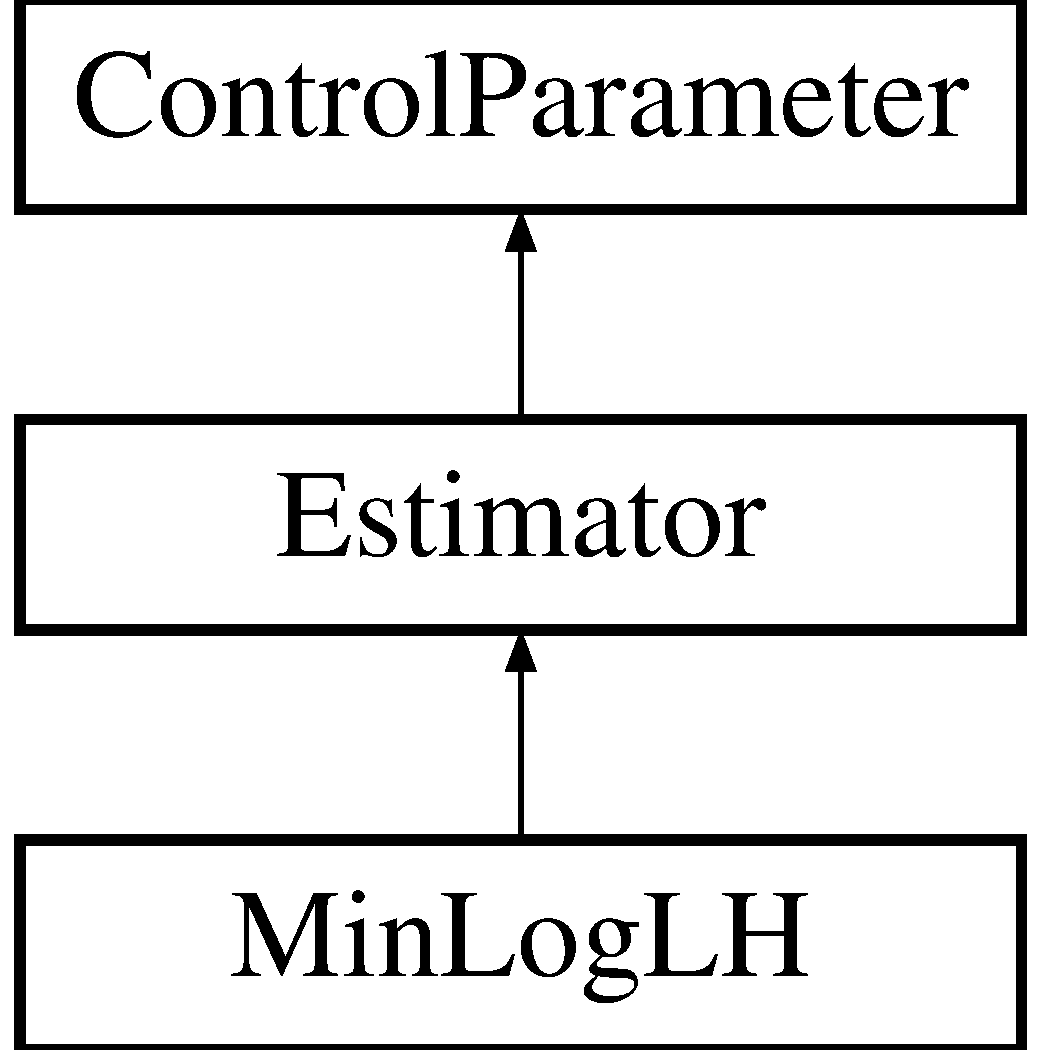
\includegraphics[height=3.000000cm]{class_min_log_l_h}
\end{center}
\end{figure}
\subsection*{Public Member Functions}
\begin{DoxyCompactItemize}
\item 
\hypertarget{class_min_log_l_h_a232569dd1c39a9c8c37d0a3dac55a41c}{virtual double {\bfseries control\-Parameter} (\hyperlink{class_parameter_list}{Parameter\-List} \&min\-Par)}\label{class_min_log_l_h_a232569dd1c39a9c8c37d0a3dac55a41c}

\item 
virtual \hyperlink{class_min_log_l_h_adae6cb73f0f9922a94adf7bfd0d33f27}{$\sim$\-Min\-Log\-L\-H} ()
\end{DoxyCompactItemize}
\subsection*{Static Public Member Functions}
\begin{DoxyCompactItemize}
\item 
\hypertarget{class_min_log_l_h_a7f9371def478b503f1fd37eb919295d4}{static std\-::shared\-\_\-ptr\\*
$<$ \hyperlink{class_control_parameter}{Control\-Parameter} $>$ {\bfseries create\-Instance} (std\-::shared\-\_\-ptr$<$ \hyperlink{class_amplitude}{Amplitude} $>$, std\-::shared\-\_\-ptr$<$ \hyperlink{class_data}{Data} $>$)}\label{class_min_log_l_h_a7f9371def478b503f1fd37eb919295d4}

\item 
\hypertarget{class_min_log_l_h_a4bfe70674a1486a7d37228f393bda13e}{static std\-::shared\-\_\-ptr\\*
$<$ \hyperlink{class_control_parameter}{Control\-Parameter} $>$ {\bfseries create\-Instance} (std\-::shared\-\_\-ptr$<$ \hyperlink{class_amplitude}{Amplitude} $>$, std\-::shared\-\_\-ptr$<$ \hyperlink{class_data}{Data} $>$, std\-::shared\-\_\-ptr$<$ \hyperlink{class_data}{Data} $>$)}\label{class_min_log_l_h_a4bfe70674a1486a7d37228f393bda13e}

\end{DoxyCompactItemize}
\subsection*{Protected Member Functions}
\begin{DoxyCompactItemize}
\item 
\hypertarget{class_min_log_l_h_af21e5c4a17bcf7e9ecc33928821dddf9}{\hyperlink{class_min_log_l_h_af21e5c4a17bcf7e9ecc33928821dddf9}{Min\-Log\-L\-H} (std\-::shared\-\_\-ptr$<$ \hyperlink{class_amplitude}{Amplitude} $>$, std\-::shared\-\_\-ptr$<$ \hyperlink{class_data}{Data} $>$)}\label{class_min_log_l_h_af21e5c4a17bcf7e9ecc33928821dddf9}

\begin{DoxyCompactList}\small\item\em Default Constructor (0x0) \end{DoxyCompactList}\item 
\hypertarget{class_min_log_l_h_a326f7f62fa2ccf856dbcf64056bfe69e}{{\bfseries Min\-Log\-L\-H} (std\-::shared\-\_\-ptr$<$ \hyperlink{class_amplitude}{Amplitude} $>$, std\-::shared\-\_\-ptr$<$ \hyperlink{class_data}{Data} $>$, std\-::shared\-\_\-ptr$<$ \hyperlink{class_data}{Data} $>$)}\label{class_min_log_l_h_a326f7f62fa2ccf856dbcf64056bfe69e}

\end{DoxyCompactItemize}
\subsection*{Additional Inherited Members}


\subsection{Detailed Description}
! Negative Log Likelihood-\/\-Estimator. 

\subsection{Constructor \& Destructor Documentation}
\hypertarget{class_min_log_l_h_adae6cb73f0f9922a94adf7bfd0d33f27}{\index{Min\-Log\-L\-H@{Min\-Log\-L\-H}!$\sim$\-Min\-Log\-L\-H@{$\sim$\-Min\-Log\-L\-H}}
\index{$\sim$\-Min\-Log\-L\-H@{$\sim$\-Min\-Log\-L\-H}!MinLogLH@{Min\-Log\-L\-H}}
\subsubsection[{$\sim$\-Min\-Log\-L\-H}]{\setlength{\rightskip}{0pt plus 5cm}Min\-Log\-L\-H\-::$\sim$\-Min\-Log\-L\-H (
\begin{DoxyParamCaption}
{}
\end{DoxyParamCaption}
)\hspace{0.3cm}{\ttfamily [virtual]}}}\label{class_min_log_l_h_adae6cb73f0f9922a94adf7bfd0d33f27}
Destructor 

The documentation for this class was generated from the following files\-:\begin{DoxyCompactItemize}
\item 
Estimator/\-Min\-Log\-L\-H/\hyperlink{_min_log_l_h_8hpp}{Min\-Log\-L\-H.\-hpp}\item 
Estimator/\-Min\-Log\-L\-H/Min\-Log\-L\-H.\-cpp\end{DoxyCompactItemize}

\hypertarget{class_minuit_fcn}{\section{Minuit\-Fcn Class Reference}
\label{class_minuit_fcn}\index{Minuit\-Fcn@{Minuit\-Fcn}}
}


Minuit2 function to be optimized.  




{\ttfamily \#include $<$Minuit\-Fcn.\-hpp$>$}



\subsection{Detailed Description}
Minuit2 function to be optimized. 

The documentation for this class was generated from the following file\-:\begin{DoxyCompactItemize}
\item 
Optimizer/\-Minuit2/\hyperlink{_minuit_fcn_8hpp}{Minuit\-Fcn.\-hpp}\end{DoxyCompactItemize}

\hypertarget{class_r_o_o_t_1_1_minuit2_1_1_minuit_fcn}{\section{R\-O\-O\-T\-:\-:Minuit2\-:\-:Minuit\-Fcn Class Reference}
\label{class_r_o_o_t_1_1_minuit2_1_1_minuit_fcn}\index{R\-O\-O\-T\-::\-Minuit2\-::\-Minuit\-Fcn@{R\-O\-O\-T\-::\-Minuit2\-::\-Minuit\-Fcn}}
}
Inheritance diagram for R\-O\-O\-T\-:\-:Minuit2\-:\-:Minuit\-Fcn\-:\begin{figure}[H]
\begin{center}
\leavevmode
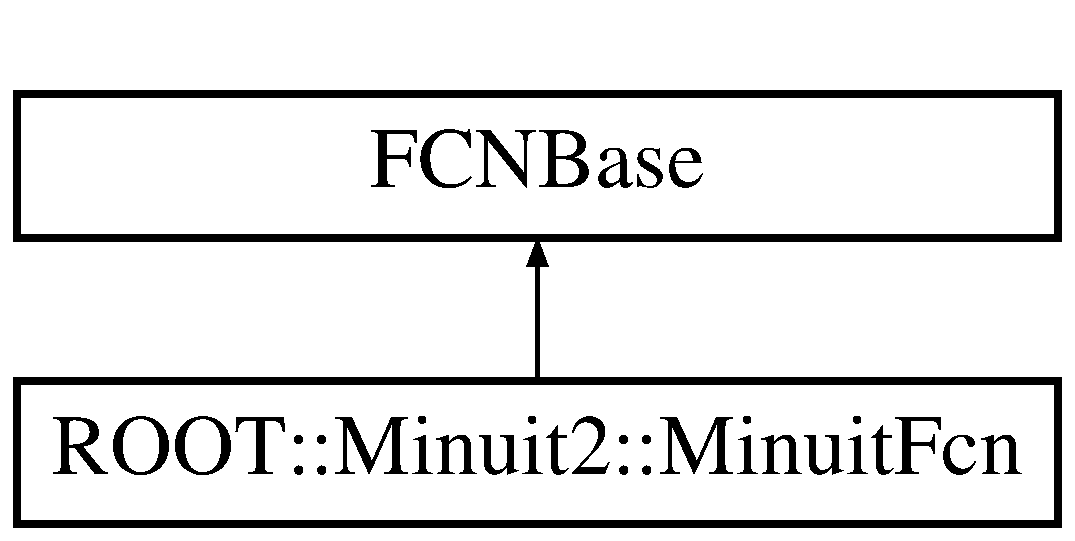
\includegraphics[height=2.000000cm]{class_r_o_o_t_1_1_minuit2_1_1_minuit_fcn}
\end{center}
\end{figure}
\subsection*{Public Member Functions}
\begin{DoxyCompactItemize}
\item 
\hypertarget{class_r_o_o_t_1_1_minuit2_1_1_minuit_fcn_a387fcbf6811bbd6e6ba97e10b1df4f10}{{\bfseries Minuit\-Fcn} (std\-::shared\-\_\-ptr$<$ \hyperlink{class_control_parameter}{Control\-Parameter} $>$ the\-Data)}\label{class_r_o_o_t_1_1_minuit2_1_1_minuit_fcn_a387fcbf6811bbd6e6ba97e10b1df4f10}

\item 
\hypertarget{class_r_o_o_t_1_1_minuit2_1_1_minuit_fcn_adb9dc1866f4f718becb2e606e7e4de6b}{double {\bfseries operator()} (const std\-::vector$<$ double $>$ \&x) const }\label{class_r_o_o_t_1_1_minuit2_1_1_minuit_fcn_adb9dc1866f4f718becb2e606e7e4de6b}

\item 
\hypertarget{class_r_o_o_t_1_1_minuit2_1_1_minuit_fcn_a66f3013fdbc34077352fe8add6620d60}{double {\bfseries Up} () const }\label{class_r_o_o_t_1_1_minuit2_1_1_minuit_fcn_a66f3013fdbc34077352fe8add6620d60}

\end{DoxyCompactItemize}


The documentation for this class was generated from the following files\-:\begin{DoxyCompactItemize}
\item 
Optimizer/\-Minuit2/\hyperlink{_minuit_fcn_8hpp}{Minuit\-Fcn.\-hpp}\item 
Optimizer/\-Minuit2/Minuit\-Fcn.\-cpp\end{DoxyCompactItemize}

\hypertarget{class_minuit_i_f}{\section{Minuit\-I\-F Class Reference}
\label{class_minuit_i_f}\index{Minuit\-I\-F@{Minuit\-I\-F}}
}


Wrapper of the Minuit2 \hyperlink{class_optimizer}{Optimizer} library.  




{\ttfamily \#include $<$Minuit\-I\-F.\-hpp$>$}

Inheritance diagram for Minuit\-I\-F\-:\begin{figure}[H]
\begin{center}
\leavevmode
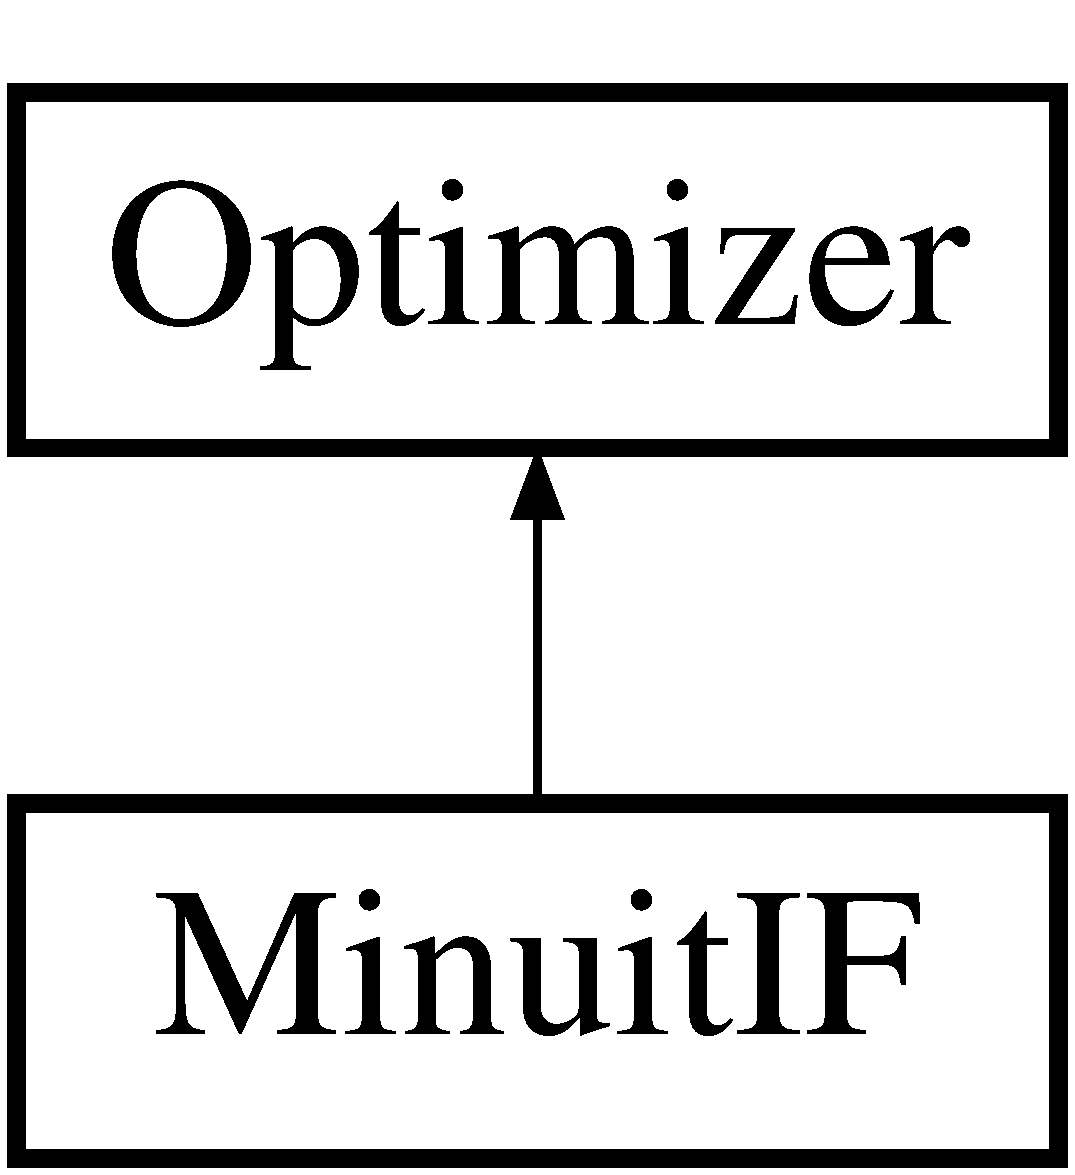
\includegraphics[height=2.000000cm]{class_minuit_i_f}
\end{center}
\end{figure}
\subsection*{Public Member Functions}
\begin{DoxyCompactItemize}
\item 
\hypertarget{class_minuit_i_f_a5c028396ab6a986ab35769fc8376cad8}{\hyperlink{class_minuit_i_f_a5c028396ab6a986ab35769fc8376cad8}{Minuit\-I\-F} (std\-::shared\-\_\-ptr$<$ \hyperlink{class_control_parameter}{Control\-Parameter} $>$ the\-Data)}\label{class_minuit_i_f_a5c028396ab6a986ab35769fc8376cad8}

\begin{DoxyCompactList}\small\item\em Default Constructor (0x0) \end{DoxyCompactList}\item 
\hypertarget{class_minuit_i_f_a3d4d3722bafc5928e6fbff32b1e6072e}{virtual const double {\bfseries exec} (\hyperlink{class_parameter_list}{Parameter\-List} \&par)}\label{class_minuit_i_f_a3d4d3722bafc5928e6fbff32b1e6072e}

\item 
virtual \hyperlink{class_minuit_i_f_a922922a4e2463dde4d4fccd0c667f588}{$\sim$\-Minuit\-I\-F} ()
\end{DoxyCompactItemize}


\subsection{Detailed Description}
Wrapper of the Minuit2 \hyperlink{class_optimizer}{Optimizer} library. 

\subsection{Constructor \& Destructor Documentation}
\hypertarget{class_minuit_i_f_a922922a4e2463dde4d4fccd0c667f588}{\index{Minuit\-I\-F@{Minuit\-I\-F}!$\sim$\-Minuit\-I\-F@{$\sim$\-Minuit\-I\-F}}
\index{$\sim$\-Minuit\-I\-F@{$\sim$\-Minuit\-I\-F}!MinuitIF@{Minuit\-I\-F}}
\subsubsection[{$\sim$\-Minuit\-I\-F}]{\setlength{\rightskip}{0pt plus 5cm}Minuit\-I\-F\-::$\sim$\-Minuit\-I\-F (
\begin{DoxyParamCaption}
{}
\end{DoxyParamCaption}
)\hspace{0.3cm}{\ttfamily [virtual]}}}\label{class_minuit_i_f_a922922a4e2463dde4d4fccd0c667f588}
Destructor 

The documentation for this class was generated from the following files\-:\begin{DoxyCompactItemize}
\item 
Optimizer/\-Minuit2/\hyperlink{_minuit_i_f_8hpp}{Minuit\-I\-F.\-hpp}\item 
Optimizer/\-Minuit2/Minuit\-I\-F.\-cpp\end{DoxyCompactItemize}

\hypertarget{class_optimizer}{\section{Optimizer Class Reference}
\label{class_optimizer}\index{Optimizer@{Optimizer}}
}


\hyperlink{class_optimizer}{Optimizer} Interface Base-\/\-Class.  




{\ttfamily \#include $<$Optimizer.\-hpp$>$}

Inheritance diagram for Optimizer\-:\begin{figure}[H]
\begin{center}
\leavevmode
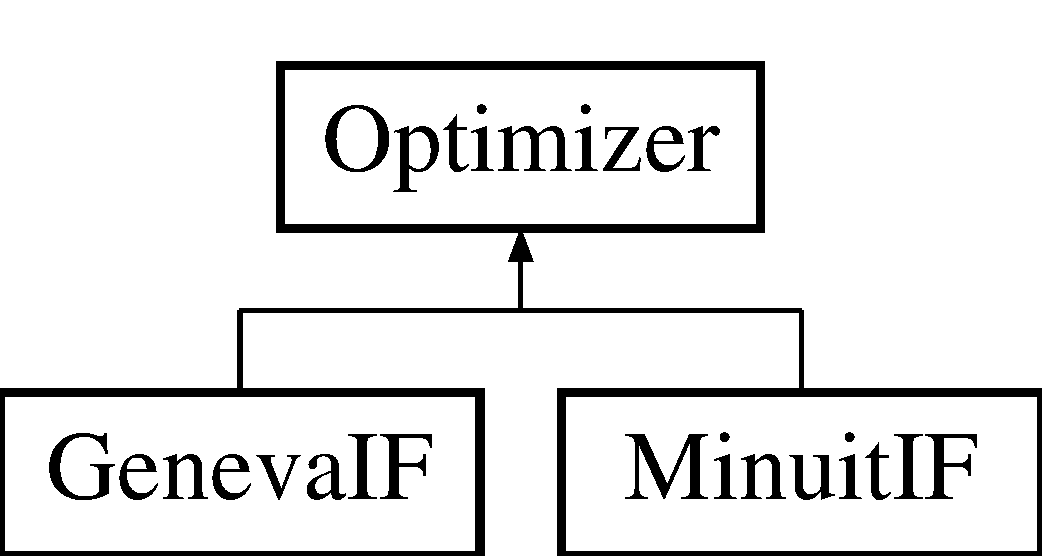
\includegraphics[height=2.000000cm]{class_optimizer}
\end{center}
\end{figure}
\subsection*{Public Member Functions}
\begin{DoxyCompactItemize}
\item 
\hypertarget{class_optimizer_a45b0eab87396b95a86c4b4adddc9cb49}{virtual const double {\bfseries exec} (\hyperlink{class_parameter_list}{Parameter\-List} \&par)=0}\label{class_optimizer_a45b0eab87396b95a86c4b4adddc9cb49}

\end{DoxyCompactItemize}


\subsection{Detailed Description}
\hyperlink{class_optimizer}{Optimizer} Interface Base-\/\-Class. 

The documentation for this class was generated from the following file\-:\begin{DoxyCompactItemize}
\item 
Optimizer/\hyperlink{_optimizer_8hpp}{Optimizer.\-hpp}\end{DoxyCompactItemize}

\hypertarget{class_parameter_fixed}{\section{Parameter\-Fixed Class Reference}
\label{class_parameter_fixed}\index{Parameter\-Fixed@{Parameter\-Fixed}}
}


Parameter cannot be changed.  




{\ttfamily \#include $<$Exceptions.\-hpp$>$}

Inheritance diagram for Parameter\-Fixed\-:\begin{figure}[H]
\begin{center}
\leavevmode
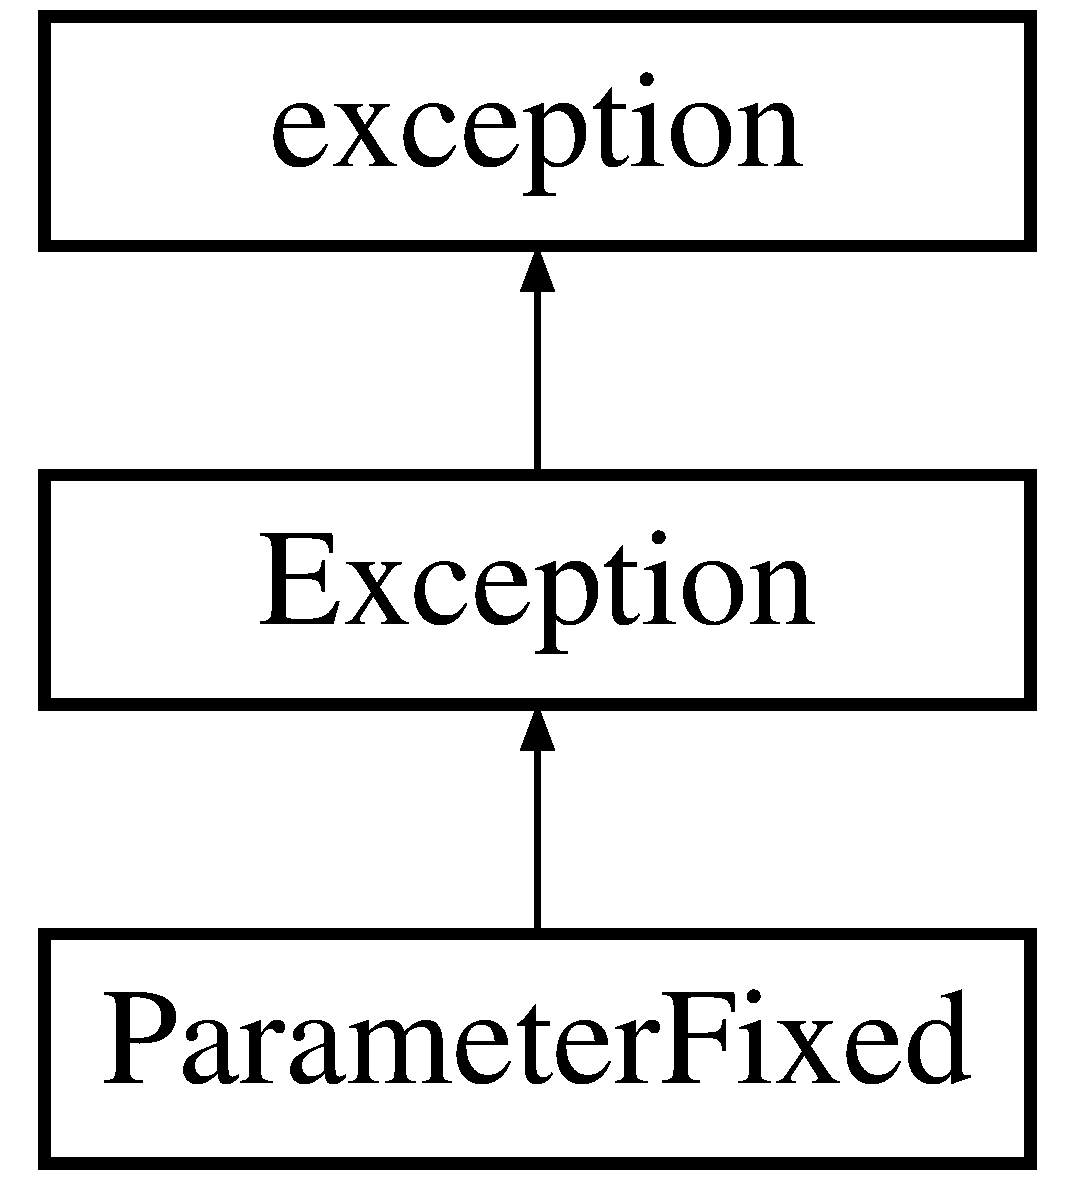
\includegraphics[height=3.000000cm]{class_parameter_fixed}
\end{center}
\end{figure}
\subsection*{Public Member Functions}
\begin{DoxyCompactItemize}
\item 
\hypertarget{class_parameter_fixed_a8cf94b1291ddf3f3cfc141cec838bc76}{{\bfseries Parameter\-Fixed} (const std\-::string \&error=\char`\"{}Parameter fixed\char`\"{})}\label{class_parameter_fixed_a8cf94b1291ddf3f3cfc141cec838bc76}

\item 
\hypertarget{class_parameter_fixed_a9c2d90f71393ad23e89219a791b24d5e}{{\bfseries Parameter\-Fixed} (const char $\ast$error)}\label{class_parameter_fixed_a9c2d90f71393ad23e89219a791b24d5e}

\end{DoxyCompactItemize}
\subsection*{Additional Inherited Members}


\subsection{Detailed Description}
Parameter cannot be changed. 

The documentation for this class was generated from the following file\-:\begin{DoxyCompactItemize}
\item 
Core/Exceptions.\-hpp\end{DoxyCompactItemize}

\hypertarget{class_parameter_list}{\section{Parameter\-List Class Reference}
\label{class_parameter_list}\index{Parameter\-List@{Parameter\-List}}
}


Internal container representing a parameter list.  




{\ttfamily \#include $<$Parameter\-List.\-hpp$>$}

\subsection*{Public Member Functions}
\begin{DoxyCompactItemize}
\item 
\hyperlink{class_parameter_list_a81cb788ca476171256c82f0416b584c6}{Parameter\-List} ()
\begin{DoxyCompactList}\small\item\em Standard constructor with empty parameter vector. \end{DoxyCompactList}\item 
\hyperlink{class_parameter_list_ab33e6f5f5f766af5ecfb4241be0f4f78}{Parameter\-List} (const std\-::vector$<$ \hyperlink{class_double_parameter}{Double\-Parameter} $>$ \&in\-Vec)
\begin{DoxyCompactList}\small\item\em Standard constructor with a vector of \hyperlink{class_double_parameter}{Double\-Parameter}. \end{DoxyCompactList}\item 
\hyperlink{class_parameter_list_a7253d65f60c0b981ea59038b64c1632b}{Parameter\-List} (const std\-::vector$<$ \hyperlink{class_integer_parameter}{Integer\-Parameter} $>$ \&in\-Vec)
\begin{DoxyCompactList}\small\item\em Standard constructor with a vector of \hyperlink{class_integer_parameter}{Integer\-Parameter}. \end{DoxyCompactList}\item 
\hyperlink{class_parameter_list_aaeac52b9c62c25950d1d7f3e83ce4213}{Parameter\-List} (const std\-::vector$<$ \hyperlink{class_bool_parameter}{Bool\-Parameter} $>$ \&in\-Vec)
\begin{DoxyCompactList}\small\item\em Standard constructor with a vector of \hyperlink{class_bool_parameter}{Bool\-Parameter}. \end{DoxyCompactList}\item 
\hyperlink{class_parameter_list_ad66b91346d298714c5200ffe658d841c}{Parameter\-List} (const std\-::vector$<$ \hyperlink{class_double_parameter}{Double\-Parameter} $>$ \&in\-D, const std\-::vector$<$ \hyperlink{class_integer_parameter}{Integer\-Parameter} $>$ \&in\-I, const std\-::vector$<$ \hyperlink{class_bool_parameter}{Bool\-Parameter} $>$ \&in\-B)
\begin{DoxyCompactList}\small\item\em Standard constructor with a vector of bool, int and double P\-W\-A\-Parameter. \end{DoxyCompactList}\item 
\hyperlink{class_parameter_list_a93bfa4961eab456b33f0009e7a5ab1bb}{Parameter\-List} (const \hyperlink{class_parameter_list}{Parameter\-List} \&in)
\begin{DoxyCompactList}\small\item\em Copy constructor using = operator. \end{DoxyCompactList}\item 
virtual \hyperlink{class_parameter_list_ad3184442bd4735ef5afbb8f7cd7b8726}{$\sim$\-Parameter\-List} ()
\begin{DoxyCompactList}\small\item\em Empty Destructor. \end{DoxyCompactList}\item 
\hypertarget{class_parameter_list_a3f27ba4154586dfb2d4c4c30d576219c}{virtual const unsigned int \hyperlink{class_parameter_list_a3f27ba4154586dfb2d4c4c30d576219c}{Get\-N\-Parameter} () const }\label{class_parameter_list_a3f27ba4154586dfb2d4c4c30d576219c}

\begin{DoxyCompactList}\small\item\em Getter for number of parameter. \end{DoxyCompactList}\item 
\hypertarget{class_parameter_list_aa626799b903b16e7f6f29f918c626f9e}{virtual const unsigned int \hyperlink{class_parameter_list_aa626799b903b16e7f6f29f918c626f9e}{Get\-N\-Double} () const }\label{class_parameter_list_aa626799b903b16e7f6f29f918c626f9e}

\begin{DoxyCompactList}\small\item\em Getter for number of double parameter. \end{DoxyCompactList}\item 
\hypertarget{class_parameter_list_a8f9f2b28594a1055ea5f8e920ebcbff7}{virtual const unsigned int \hyperlink{class_parameter_list_a8f9f2b28594a1055ea5f8e920ebcbff7}{Get\-N\-Integer} () const }\label{class_parameter_list_a8f9f2b28594a1055ea5f8e920ebcbff7}

\begin{DoxyCompactList}\small\item\em Getter for number of integer parameter. \end{DoxyCompactList}\item 
\hypertarget{class_parameter_list_a5c21a1598d5c0bf2f864f4bb10484313}{virtual const unsigned int \hyperlink{class_parameter_list_a5c21a1598d5c0bf2f864f4bb10484313}{Get\-N\-Bool} () const }\label{class_parameter_list_a5c21a1598d5c0bf2f864f4bb10484313}

\begin{DoxyCompactList}\small\item\em Getter for number of boolean parameter. \end{DoxyCompactList}\item 
virtual \hyperlink{class_double_parameter}{Double\-Parameter} \& \hyperlink{class_parameter_list_a5fd405f70ee9eb625d0ebb1a43e3b126}{Get\-Double\-Parameter} (const unsigned int i)
\begin{DoxyCompactList}\small\item\em Getter for floating point parameter. \end{DoxyCompactList}\item 
virtual \hyperlink{class_integer_parameter}{Integer\-Parameter} \& \hyperlink{class_parameter_list_a4a0f112557a3a9fada4aee97118ff1de}{Get\-Integer\-Parameter} (const unsigned int i)
\begin{DoxyCompactList}\small\item\em Getter for integer parameter. \end{DoxyCompactList}\item 
virtual \hyperlink{class_bool_parameter}{Bool\-Parameter} \& \hyperlink{class_parameter_list_a3982c7d4706e2115eed776e4b08268fb}{Get\-Bool\-Parameter} (const unsigned int i)
\begin{DoxyCompactList}\small\item\em Getter for boolean parameter. \end{DoxyCompactList}\item 
virtual const double \hyperlink{class_parameter_list_a99c664620aa97bc31d1defcf7ab4c927}{Get\-Parameter\-Value} (const unsigned int i) const 
\begin{DoxyCompactList}\small\item\em Getter for parameter value. \end{DoxyCompactList}\item 
virtual void \hyperlink{class_parameter_list_ad88a26efd71e1d3d65924500b72ffd61}{Set\-Parameter\-Value} (const unsigned int i, const double in\-Val)
\begin{DoxyCompactList}\small\item\em Setter for parameter value. \end{DoxyCompactList}\item 
virtual void \hyperlink{class_parameter_list_afefffdda9cf6dfd97a519baa0e1f6e5b}{Set\-Parameter\-Value} (const unsigned int i, const int in\-Val)
\begin{DoxyCompactList}\small\item\em Setter for parameter value. \end{DoxyCompactList}\item 
virtual void \hyperlink{class_parameter_list_a41192da59a56f939d1149a00cadfc6b3}{Set\-Parameter\-Value} (const unsigned int i, const bool in\-Val)
\begin{DoxyCompactList}\small\item\em Setter for parameter value. \end{DoxyCompactList}\item 
virtual void \hyperlink{class_parameter_list_a0d5088fbb4fb10a3efea998d1aeee1a3}{Add\-Parameter} (\hyperlink{class_double_parameter}{Double\-Parameter} par)
\begin{DoxyCompactList}\small\item\em Add floating point parameter. \end{DoxyCompactList}\item 
virtual void \hyperlink{class_parameter_list_a817d794256d9f2e0f38535c264b2761b}{Add\-Parameter} (\hyperlink{class_integer_parameter}{Integer\-Parameter} par)
\begin{DoxyCompactList}\small\item\em Add integer parameter. \end{DoxyCompactList}\item 
virtual void \hyperlink{class_parameter_list_a7fb0ec39de4c17fd0a9d3805673007d4}{Add\-Parameter} (\hyperlink{class_bool_parameter}{Bool\-Parameter} par)
\begin{DoxyCompactList}\small\item\em Add boolean parameter. \end{DoxyCompactList}\item 
std\-::string const \& \hyperlink{class_parameter_list_a9ea8f819a48dd707785e2db937736bd5}{to\-\_\-str} () const 
\begin{DoxyCompactList}\small\item\em A public function returning a string with parameter information. \end{DoxyCompactList}\end{DoxyCompactItemize}
\subsection*{Protected Member Functions}
\begin{DoxyCompactItemize}
\item 
void \hyperlink{class_parameter_list_ac93259ed7c23cfcc73e906664ba2159a}{make\-\_\-str} ()
\begin{DoxyCompactList}\small\item\em A protected function which creates an output string for printing. \end{DoxyCompactList}\end{DoxyCompactItemize}
\subsection*{Protected Attributes}
\begin{DoxyCompactItemize}
\item 
std\-::vector$<$ \hyperlink{class_double_parameter}{Double\-Parameter} $>$ \hyperlink{class_parameter_list_ae2c308362f7b1f3ea063677d2e28ad3c}{v\-Double\-Par\-\_\-}
\item 
std\-::vector$<$ \hyperlink{class_integer_parameter}{Integer\-Parameter} $>$ \hyperlink{class_parameter_list_a9398a16845891a6cf22230771636b439}{v\-Int\-Par\-\_\-}
\item 
std\-::vector$<$ \hyperlink{class_bool_parameter}{Bool\-Parameter} $>$ \hyperlink{class_parameter_list_a71da57a577ae374300d2b30c3481bccd}{v\-Bool\-Par\-\_\-}
\item 
std\-::string \hyperlink{class_parameter_list_a8091ca235596882df0e06a3fcd5345c6}{out\-\_\-}
\end{DoxyCompactItemize}
\subsection*{Friends}
\begin{DoxyCompactItemize}
\item 
std\-::ostream \& \hyperlink{class_parameter_list_a7a23c0f7036c113aed95092096453d65}{operator$<$$<$} (std\-::ostream \&os, const \hyperlink{class_parameter_list}{Parameter\-List} \&p)
\begin{DoxyCompactList}\small\item\em friend function to stream parameter information to output \end{DoxyCompactList}\end{DoxyCompactItemize}


\subsection{Detailed Description}
Internal container representing a parameter list. 

\subsection{Constructor \& Destructor Documentation}
\hypertarget{class_parameter_list_a81cb788ca476171256c82f0416b584c6}{\index{Parameter\-List@{Parameter\-List}!Parameter\-List@{Parameter\-List}}
\index{Parameter\-List@{Parameter\-List}!ParameterList@{Parameter\-List}}
\subsubsection[{Parameter\-List}]{\setlength{\rightskip}{0pt plus 5cm}Parameter\-List\-::\-Parameter\-List (
\begin{DoxyParamCaption}
{}
\end{DoxyParamCaption}
)}}\label{class_parameter_list_a81cb788ca476171256c82f0416b584c6}


Standard constructor with empty parameter vector. 

Standard constructor without input. The vectors of parameters are empty. \hypertarget{class_parameter_list_ab33e6f5f5f766af5ecfb4241be0f4f78}{\index{Parameter\-List@{Parameter\-List}!Parameter\-List@{Parameter\-List}}
\index{Parameter\-List@{Parameter\-List}!ParameterList@{Parameter\-List}}
\subsubsection[{Parameter\-List}]{\setlength{\rightskip}{0pt plus 5cm}Parameter\-List\-::\-Parameter\-List (
\begin{DoxyParamCaption}
\item[{const std\-::vector$<$ {\bf Double\-Parameter} $>$ \&}]{in\-Vec}
\end{DoxyParamCaption}
)}}\label{class_parameter_list_ab33e6f5f5f766af5ecfb4241be0f4f78}


Standard constructor with a vector of \hyperlink{class_double_parameter}{Double\-Parameter}. 

Standard constructor with list of P\-W\-A\-Parameter provided. The vector gets copied to the internal vector. To avoid copying, use the add\-Parameter() functions and empty constructor P\-W\-A\-Parameter\-List. Non-\/double parameter are empty 
\begin{DoxyParams}{Parameters}
{\em in\-Vec} & input vector of double parameters \\
\hline
\end{DoxyParams}
\begin{DoxySeeAlso}{See Also}
add\-Parameter(\-P\-W\-A\-Parameter$<$double$>$\&) 
\end{DoxySeeAlso}
\hypertarget{class_parameter_list_a7253d65f60c0b981ea59038b64c1632b}{\index{Parameter\-List@{Parameter\-List}!Parameter\-List@{Parameter\-List}}
\index{Parameter\-List@{Parameter\-List}!ParameterList@{Parameter\-List}}
\subsubsection[{Parameter\-List}]{\setlength{\rightskip}{0pt plus 5cm}Parameter\-List\-::\-Parameter\-List (
\begin{DoxyParamCaption}
\item[{const std\-::vector$<$ {\bf Integer\-Parameter} $>$ \&}]{in\-Vec}
\end{DoxyParamCaption}
)}}\label{class_parameter_list_a7253d65f60c0b981ea59038b64c1632b}


Standard constructor with a vector of \hyperlink{class_integer_parameter}{Integer\-Parameter}. 

Standard constructor with list of P\-W\-A\-Parameter provided. The vector gets copied to the internal vector. To avoid copying, use the add\-Parameter() functions and empty constructor P\-W\-A\-Parameter\-List. Non-\/integer parameter are empty 
\begin{DoxyParams}{Parameters}
{\em in\-Vec} & input vector of integer parameters \\
\hline
\end{DoxyParams}
\begin{DoxySeeAlso}{See Also}
add\-Parameter(\-P\-W\-A\-Parameter$<$integer$>$\&) 
\end{DoxySeeAlso}
\hypertarget{class_parameter_list_aaeac52b9c62c25950d1d7f3e83ce4213}{\index{Parameter\-List@{Parameter\-List}!Parameter\-List@{Parameter\-List}}
\index{Parameter\-List@{Parameter\-List}!ParameterList@{Parameter\-List}}
\subsubsection[{Parameter\-List}]{\setlength{\rightskip}{0pt plus 5cm}Parameter\-List\-::\-Parameter\-List (
\begin{DoxyParamCaption}
\item[{const std\-::vector$<$ {\bf Bool\-Parameter} $>$ \&}]{in\-Vec}
\end{DoxyParamCaption}
)}}\label{class_parameter_list_aaeac52b9c62c25950d1d7f3e83ce4213}


Standard constructor with a vector of \hyperlink{class_bool_parameter}{Bool\-Parameter}. 

Standard constructor with list of P\-W\-A\-Parameter provided. The vector gets copied to the internal vector. To avoid copying, use the add\-Parameter() functions and empty constructor P\-W\-A\-Parameter\-List. Non-\/boolean parameter are empty 
\begin{DoxyParams}{Parameters}
{\em in\-Vec} & input vector of boolean parameters \\
\hline
\end{DoxyParams}
\begin{DoxySeeAlso}{See Also}
add\-Parameter(\-P\-W\-A\-Parameter$<$bool$>$\&) 
\end{DoxySeeAlso}
\hypertarget{class_parameter_list_ad66b91346d298714c5200ffe658d841c}{\index{Parameter\-List@{Parameter\-List}!Parameter\-List@{Parameter\-List}}
\index{Parameter\-List@{Parameter\-List}!ParameterList@{Parameter\-List}}
\subsubsection[{Parameter\-List}]{\setlength{\rightskip}{0pt plus 5cm}Parameter\-List\-::\-Parameter\-List (
\begin{DoxyParamCaption}
\item[{const std\-::vector$<$ {\bf Double\-Parameter} $>$ \&}]{in\-D, }
\item[{const std\-::vector$<$ {\bf Integer\-Parameter} $>$ \&}]{in\-I, }
\item[{const std\-::vector$<$ {\bf Bool\-Parameter} $>$ \&}]{in\-B}
\end{DoxyParamCaption}
)}}\label{class_parameter_list_ad66b91346d298714c5200ffe658d841c}


Standard constructor with a vector of bool, int and double P\-W\-A\-Parameter. 

Standard constructor with list of P\-W\-A\-Parameter provided. The vectors get copied to the internal vectors. To avoid copying, use the add\-Parameter() functions and empty constructor P\-W\-A\-Parameter\-List. 
\begin{DoxyParams}{Parameters}
{\em in\-D} & input vector of floating point parameters \\
\hline
{\em in\-I} & input vector of integer parameters \\
\hline
{\em in\-B} & input vector of boolean parameters \\
\hline
\end{DoxyParams}
\begin{DoxySeeAlso}{See Also}
add\-Parameter(\-P\-W\-A\-Parameter$<$double$>$\&, P\-W\-A\-Parameter$<$int$>$\&, P\-W\-A\-Parameter$<$bool$>$\&) 
\end{DoxySeeAlso}
\hypertarget{class_parameter_list_a93bfa4961eab456b33f0009e7a5ab1bb}{\index{Parameter\-List@{Parameter\-List}!Parameter\-List@{Parameter\-List}}
\index{Parameter\-List@{Parameter\-List}!ParameterList@{Parameter\-List}}
\subsubsection[{Parameter\-List}]{\setlength{\rightskip}{0pt plus 5cm}Parameter\-List\-::\-Parameter\-List (
\begin{DoxyParamCaption}
\item[{const {\bf Parameter\-List} \&}]{in}
\end{DoxyParamCaption}
)}}\label{class_parameter_list_a93bfa4961eab456b33f0009e7a5ab1bb}


Copy constructor using = operator. 

Simple copy constructor using the = operator. As this operator is not overloaded in this class, c++ will copy every member variable. As this is a container class, this should be fine. 
\begin{DoxyParams}{Parameters}
{\em in} & input P\-W\-A\-Parameter\-List which variables will be copied \\
\hline
\end{DoxyParams}
\hypertarget{class_parameter_list_ad3184442bd4735ef5afbb8f7cd7b8726}{\index{Parameter\-List@{Parameter\-List}!$\sim$\-Parameter\-List@{$\sim$\-Parameter\-List}}
\index{$\sim$\-Parameter\-List@{$\sim$\-Parameter\-List}!ParameterList@{Parameter\-List}}
\subsubsection[{$\sim$\-Parameter\-List}]{\setlength{\rightskip}{0pt plus 5cm}Parameter\-List\-::$\sim$\-Parameter\-List (
\begin{DoxyParamCaption}
{}
\end{DoxyParamCaption}
)\hspace{0.3cm}{\ttfamily [virtual]}}}\label{class_parameter_list_ad3184442bd4735ef5afbb8f7cd7b8726}


Empty Destructor. 

There is nothing to destroy \-:( 

\subsection{Member Function Documentation}
\hypertarget{class_parameter_list_a0d5088fbb4fb10a3efea998d1aeee1a3}{\index{Parameter\-List@{Parameter\-List}!Add\-Parameter@{Add\-Parameter}}
\index{Add\-Parameter@{Add\-Parameter}!ParameterList@{Parameter\-List}}
\subsubsection[{Add\-Parameter}]{\setlength{\rightskip}{0pt plus 5cm}void Parameter\-List\-::\-Add\-Parameter (
\begin{DoxyParamCaption}
\item[{{\bf Double\-Parameter}}]{par}
\end{DoxyParamCaption}
)\hspace{0.3cm}{\ttfamily [virtual]}}}\label{class_parameter_list_a0d5088fbb4fb10a3efea998d1aeee1a3}


Add floating point parameter. 

Adds a floating point parameter to the list 
\begin{DoxyParams}{Parameters}
{\em par} & input parameter \\
\hline
\end{DoxyParams}
\hypertarget{class_parameter_list_a817d794256d9f2e0f38535c264b2761b}{\index{Parameter\-List@{Parameter\-List}!Add\-Parameter@{Add\-Parameter}}
\index{Add\-Parameter@{Add\-Parameter}!ParameterList@{Parameter\-List}}
\subsubsection[{Add\-Parameter}]{\setlength{\rightskip}{0pt plus 5cm}void Parameter\-List\-::\-Add\-Parameter (
\begin{DoxyParamCaption}
\item[{{\bf Integer\-Parameter}}]{par}
\end{DoxyParamCaption}
)\hspace{0.3cm}{\ttfamily [virtual]}}}\label{class_parameter_list_a817d794256d9f2e0f38535c264b2761b}


Add integer parameter. 

Adds an integer parameter to the list 
\begin{DoxyParams}{Parameters}
{\em par} & input parameter \\
\hline
\end{DoxyParams}
\hypertarget{class_parameter_list_a7fb0ec39de4c17fd0a9d3805673007d4}{\index{Parameter\-List@{Parameter\-List}!Add\-Parameter@{Add\-Parameter}}
\index{Add\-Parameter@{Add\-Parameter}!ParameterList@{Parameter\-List}}
\subsubsection[{Add\-Parameter}]{\setlength{\rightskip}{0pt plus 5cm}void Parameter\-List\-::\-Add\-Parameter (
\begin{DoxyParamCaption}
\item[{{\bf Bool\-Parameter}}]{par}
\end{DoxyParamCaption}
)\hspace{0.3cm}{\ttfamily [virtual]}}}\label{class_parameter_list_a7fb0ec39de4c17fd0a9d3805673007d4}


Add boolean parameter. 

Adds an boolean parameter to the list 
\begin{DoxyParams}{Parameters}
{\em par} & input parameter \\
\hline
\end{DoxyParams}
\hypertarget{class_parameter_list_a3982c7d4706e2115eed776e4b08268fb}{\index{Parameter\-List@{Parameter\-List}!Get\-Bool\-Parameter@{Get\-Bool\-Parameter}}
\index{Get\-Bool\-Parameter@{Get\-Bool\-Parameter}!ParameterList@{Parameter\-List}}
\subsubsection[{Get\-Bool\-Parameter}]{\setlength{\rightskip}{0pt plus 5cm}{\bf Bool\-Parameter} \& Parameter\-List\-::\-Get\-Bool\-Parameter (
\begin{DoxyParamCaption}
\item[{const unsigned int}]{i}
\end{DoxyParamCaption}
)\hspace{0.3cm}{\ttfamily [virtual]}}}\label{class_parameter_list_a3982c7d4706e2115eed776e4b08268fb}


Getter for boolean parameter. 

Getter for boolean parameter 
\begin{DoxyParams}{Parameters}
{\em i} & input number of parameter to load \\
\hline
\end{DoxyParams}
\begin{DoxyReturn}{Returns}
par output container for loaded parameter 
\end{DoxyReturn}
\hypertarget{class_parameter_list_a5fd405f70ee9eb625d0ebb1a43e3b126}{\index{Parameter\-List@{Parameter\-List}!Get\-Double\-Parameter@{Get\-Double\-Parameter}}
\index{Get\-Double\-Parameter@{Get\-Double\-Parameter}!ParameterList@{Parameter\-List}}
\subsubsection[{Get\-Double\-Parameter}]{\setlength{\rightskip}{0pt plus 5cm}{\bf Double\-Parameter} \& Parameter\-List\-::\-Get\-Double\-Parameter (
\begin{DoxyParamCaption}
\item[{const unsigned int}]{i}
\end{DoxyParamCaption}
)\hspace{0.3cm}{\ttfamily [virtual]}}}\label{class_parameter_list_a5fd405f70ee9eb625d0ebb1a43e3b126}


Getter for floating point parameter. 

Getter for floating point parameter 
\begin{DoxyParams}{Parameters}
{\em i} & input number of parameter to load \\
\hline
\end{DoxyParams}
\begin{DoxyReturn}{Returns}
par output container for loaded parameter 
\end{DoxyReturn}
\hypertarget{class_parameter_list_a4a0f112557a3a9fada4aee97118ff1de}{\index{Parameter\-List@{Parameter\-List}!Get\-Integer\-Parameter@{Get\-Integer\-Parameter}}
\index{Get\-Integer\-Parameter@{Get\-Integer\-Parameter}!ParameterList@{Parameter\-List}}
\subsubsection[{Get\-Integer\-Parameter}]{\setlength{\rightskip}{0pt plus 5cm}{\bf Integer\-Parameter} \& Parameter\-List\-::\-Get\-Integer\-Parameter (
\begin{DoxyParamCaption}
\item[{const unsigned int}]{i}
\end{DoxyParamCaption}
)\hspace{0.3cm}{\ttfamily [virtual]}}}\label{class_parameter_list_a4a0f112557a3a9fada4aee97118ff1de}


Getter for integer parameter. 

Getter for integer parameter 
\begin{DoxyParams}{Parameters}
{\em i} & input number of parameter to load \\
\hline
\end{DoxyParams}
\begin{DoxyReturn}{Returns}
par output container for loaded parameter 
\end{DoxyReturn}
\hypertarget{class_parameter_list_a99c664620aa97bc31d1defcf7ab4c927}{\index{Parameter\-List@{Parameter\-List}!Get\-Parameter\-Value@{Get\-Parameter\-Value}}
\index{Get\-Parameter\-Value@{Get\-Parameter\-Value}!ParameterList@{Parameter\-List}}
\subsubsection[{Get\-Parameter\-Value}]{\setlength{\rightskip}{0pt plus 5cm}const double Parameter\-List\-::\-Get\-Parameter\-Value (
\begin{DoxyParamCaption}
\item[{const unsigned int}]{i}
\end{DoxyParamCaption}
) const\hspace{0.3cm}{\ttfamily [virtual]}}}\label{class_parameter_list_a99c664620aa97bc31d1defcf7ab4c927}


Getter for parameter value. 

Getter for parameter value 
\begin{DoxyParams}{Parameters}
{\em i} & input number of parameter to load \\
\hline
\end{DoxyParams}
\begin{DoxyReturn}{Returns}
par output container for loaded parameter 
\end{DoxyReturn}
\hypertarget{class_parameter_list_ac93259ed7c23cfcc73e906664ba2159a}{\index{Parameter\-List@{Parameter\-List}!make\-\_\-str@{make\-\_\-str}}
\index{make\-\_\-str@{make\-\_\-str}!ParameterList@{Parameter\-List}}
\subsubsection[{make\-\_\-str}]{\setlength{\rightskip}{0pt plus 5cm}void Parameter\-List\-::make\-\_\-str (
\begin{DoxyParamCaption}
{}
\end{DoxyParamCaption}
)\hspace{0.3cm}{\ttfamily [protected]}}}\label{class_parameter_list_ac93259ed7c23cfcc73e906664ba2159a}


A protected function which creates an output string for printing. 

This function uses all available information about the parameterlist to create a string which will be streamed via the stream operator $<$$<$. \begin{DoxySeeAlso}{See Also}
operator$<$$<$, \hyperlink{class_parameter_list_a9ea8f819a48dd707785e2db937736bd5}{to\-\_\-str()} 
\end{DoxySeeAlso}
\hypertarget{class_parameter_list_ad88a26efd71e1d3d65924500b72ffd61}{\index{Parameter\-List@{Parameter\-List}!Set\-Parameter\-Value@{Set\-Parameter\-Value}}
\index{Set\-Parameter\-Value@{Set\-Parameter\-Value}!ParameterList@{Parameter\-List}}
\subsubsection[{Set\-Parameter\-Value}]{\setlength{\rightskip}{0pt plus 5cm}void Parameter\-List\-::\-Set\-Parameter\-Value (
\begin{DoxyParamCaption}
\item[{const unsigned int}]{i, }
\item[{const double}]{in\-Val}
\end{DoxyParamCaption}
)\hspace{0.3cm}{\ttfamily [virtual]}}}\label{class_parameter_list_ad88a26efd71e1d3d65924500b72ffd61}


Setter for parameter value. 

Setter for parameter value 
\begin{DoxyParams}{Parameters}
{\em i} & input number of parameter to load \\
\hline
{\em in\-Val} & input floating value for parameter \\
\hline
\end{DoxyParams}
\hypertarget{class_parameter_list_afefffdda9cf6dfd97a519baa0e1f6e5b}{\index{Parameter\-List@{Parameter\-List}!Set\-Parameter\-Value@{Set\-Parameter\-Value}}
\index{Set\-Parameter\-Value@{Set\-Parameter\-Value}!ParameterList@{Parameter\-List}}
\subsubsection[{Set\-Parameter\-Value}]{\setlength{\rightskip}{0pt plus 5cm}void Parameter\-List\-::\-Set\-Parameter\-Value (
\begin{DoxyParamCaption}
\item[{const unsigned int}]{i, }
\item[{const int}]{in\-Val}
\end{DoxyParamCaption}
)\hspace{0.3cm}{\ttfamily [virtual]}}}\label{class_parameter_list_afefffdda9cf6dfd97a519baa0e1f6e5b}


Setter for parameter value. 

Setter for parameter value 
\begin{DoxyParams}{Parameters}
{\em i} & input number of parameter to load \\
\hline
{\em in\-Val} & input integer value for parameter \\
\hline
\end{DoxyParams}
\hypertarget{class_parameter_list_a41192da59a56f939d1149a00cadfc6b3}{\index{Parameter\-List@{Parameter\-List}!Set\-Parameter\-Value@{Set\-Parameter\-Value}}
\index{Set\-Parameter\-Value@{Set\-Parameter\-Value}!ParameterList@{Parameter\-List}}
\subsubsection[{Set\-Parameter\-Value}]{\setlength{\rightskip}{0pt plus 5cm}void Parameter\-List\-::\-Set\-Parameter\-Value (
\begin{DoxyParamCaption}
\item[{const unsigned int}]{i, }
\item[{const bool}]{in\-Val}
\end{DoxyParamCaption}
)\hspace{0.3cm}{\ttfamily [virtual]}}}\label{class_parameter_list_a41192da59a56f939d1149a00cadfc6b3}


Setter for parameter value. 

Setter for parameter value 
\begin{DoxyParams}{Parameters}
{\em i} & input number of parameter to load \\
\hline
{\em in\-Val} & input boolean value for parameter \\
\hline
\end{DoxyParams}
\hypertarget{class_parameter_list_a9ea8f819a48dd707785e2db937736bd5}{\index{Parameter\-List@{Parameter\-List}!to\-\_\-str@{to\-\_\-str}}
\index{to\-\_\-str@{to\-\_\-str}!ParameterList@{Parameter\-List}}
\subsubsection[{to\-\_\-str}]{\setlength{\rightskip}{0pt plus 5cm}std\-::string const \& Parameter\-List\-::to\-\_\-str (
\begin{DoxyParamCaption}
{}
\end{DoxyParamCaption}
) const}}\label{class_parameter_list_a9ea8f819a48dd707785e2db937736bd5}


A public function returning a string with parameter information. 

This function simply returns the member string out\-\_\-, which contains all parameter information. The string gets created using the outstream of the P\-W\-A\-Parameter class. \begin{DoxyReturn}{Returns}
string with parameter information 
\end{DoxyReturn}
\begin{DoxySeeAlso}{See Also}
operator$<$$<$ 
\end{DoxySeeAlso}


\subsection{Friends And Related Function Documentation}
\hypertarget{class_parameter_list_a7a23c0f7036c113aed95092096453d65}{\index{Parameter\-List@{Parameter\-List}!operator$<$$<$@{operator$<$$<$}}
\index{operator$<$$<$@{operator$<$$<$}!ParameterList@{Parameter\-List}}
\subsubsection[{operator$<$$<$}]{\setlength{\rightskip}{0pt plus 5cm}std\-::ostream\& operator$<$$<$ (
\begin{DoxyParamCaption}
\item[{std\-::ostream \&}]{os, }
\item[{const {\bf Parameter\-List} \&}]{p}
\end{DoxyParamCaption}
)\hspace{0.3cm}{\ttfamily [friend]}}}\label{class_parameter_list_a7a23c0f7036c113aed95092096453d65}


friend function to stream parameter information to output 

Declaring the stream-\/operator $<$$<$ as friend allows to stream parameter information to the output as easily as a generic type. The definition of this class has to be outside the namespace of the class. \begin{DoxySeeAlso}{See Also}
\hyperlink{class_parameter_list_ac93259ed7c23cfcc73e906664ba2159a}{make\-\_\-str()}, \hyperlink{class_parameter_list_a9ea8f819a48dd707785e2db937736bd5}{to\-\_\-str()} 
\end{DoxySeeAlso}


\subsection{Field Documentation}
\hypertarget{class_parameter_list_a8091ca235596882df0e06a3fcd5345c6}{\index{Parameter\-List@{Parameter\-List}!out\-\_\-@{out\-\_\-}}
\index{out\-\_\-@{out\-\_\-}!ParameterList@{Parameter\-List}}
\subsubsection[{out\-\_\-}]{\setlength{\rightskip}{0pt plus 5cm}std\-::string Parameter\-List\-::out\-\_\-\hspace{0.3cm}{\ttfamily [protected]}}}\label{class_parameter_list_a8091ca235596882df0e06a3fcd5345c6}
Output string to print information \hypertarget{class_parameter_list_a71da57a577ae374300d2b30c3481bccd}{\index{Parameter\-List@{Parameter\-List}!v\-Bool\-Par\-\_\-@{v\-Bool\-Par\-\_\-}}
\index{v\-Bool\-Par\-\_\-@{v\-Bool\-Par\-\_\-}!ParameterList@{Parameter\-List}}
\subsubsection[{v\-Bool\-Par\-\_\-}]{\setlength{\rightskip}{0pt plus 5cm}std\-::vector$<${\bf Bool\-Parameter}$>$ Parameter\-List\-::v\-Bool\-Par\-\_\-\hspace{0.3cm}{\ttfamily [protected]}}}\label{class_parameter_list_a71da57a577ae374300d2b30c3481bccd}
Vector of boolean parameters \hypertarget{class_parameter_list_ae2c308362f7b1f3ea063677d2e28ad3c}{\index{Parameter\-List@{Parameter\-List}!v\-Double\-Par\-\_\-@{v\-Double\-Par\-\_\-}}
\index{v\-Double\-Par\-\_\-@{v\-Double\-Par\-\_\-}!ParameterList@{Parameter\-List}}
\subsubsection[{v\-Double\-Par\-\_\-}]{\setlength{\rightskip}{0pt plus 5cm}std\-::vector$<${\bf Double\-Parameter}$>$ Parameter\-List\-::v\-Double\-Par\-\_\-\hspace{0.3cm}{\ttfamily [protected]}}}\label{class_parameter_list_ae2c308362f7b1f3ea063677d2e28ad3c}
Vector of floating point parameters \hypertarget{class_parameter_list_a9398a16845891a6cf22230771636b439}{\index{Parameter\-List@{Parameter\-List}!v\-Int\-Par\-\_\-@{v\-Int\-Par\-\_\-}}
\index{v\-Int\-Par\-\_\-@{v\-Int\-Par\-\_\-}!ParameterList@{Parameter\-List}}
\subsubsection[{v\-Int\-Par\-\_\-}]{\setlength{\rightskip}{0pt plus 5cm}std\-::vector$<${\bf Integer\-Parameter}$>$ Parameter\-List\-::v\-Int\-Par\-\_\-\hspace{0.3cm}{\ttfamily [protected]}}}\label{class_parameter_list_a9398a16845891a6cf22230771636b439}
Vector of integer parameters 

The documentation for this class was generated from the following files\-:\begin{DoxyCompactItemize}
\item 
Core/\hyperlink{_parameter_list_8hpp}{Parameter\-List.\-hpp}\item 
Core/Parameter\-List.\-cpp\end{DoxyCompactItemize}

\hypertarget{struct_particle}{\section{Particle Class Reference}
\label{struct_particle}\index{Particle@{Particle}}
}


Internal container representing a particle.  




{\ttfamily \#include $<$Particle.\-hpp$>$}

\subsection*{Public Member Functions}
\begin{DoxyCompactItemize}
\item 
\hypertarget{struct_particle_abc1277b6ac392f87bdb03df3c782e799}{{\bfseries Particle} (double in\-Px, double in\-Py, double in\-Pz, double in\-E, int inpid=0)}\label{struct_particle_abc1277b6ac392f87bdb03df3c782e799}

\item 
\hypertarget{struct_particle_ab6007fd3a3794808270afceb50d52df0}{{\bfseries Particle} (const \hyperlink{struct_particle}{Particle} \&in\-Particle)}\label{struct_particle_ab6007fd3a3794808270afceb50d52df0}

\item 
\hypertarget{struct_particle_a9b1160ecde77b56dd41adf591af897d4}{double {\bfseries invariant\-Mass} (const \hyperlink{struct_particle}{Particle} \&in\-Particle) const }\label{struct_particle_a9b1160ecde77b56dd41adf591af897d4}

\end{DoxyCompactItemize}
\subsection*{Static Public Member Functions}
\begin{DoxyCompactItemize}
\item 
\hypertarget{struct_particle_a1369d604579dea453eea62660ab759bf}{static double {\bfseries invariant\-Mass} (const \hyperlink{struct_particle}{Particle} \&in\-Pa, const \hyperlink{struct_particle}{Particle} \&in\-Pb)}\label{struct_particle_a1369d604579dea453eea62660ab759bf}

\end{DoxyCompactItemize}
\subsection*{Data Fields}
\begin{DoxyCompactItemize}
\item 
\hypertarget{struct_particle_a2b4a2387122f9029548de4c237e2c9c6}{double {\bfseries px}}\label{struct_particle_a2b4a2387122f9029548de4c237e2c9c6}

\item 
\hypertarget{struct_particle_a520405a04f53ac2602801385d2290e1b}{double {\bfseries py}}\label{struct_particle_a520405a04f53ac2602801385d2290e1b}

\item 
\hypertarget{struct_particle_ad3e28a3b7126f0fcc1ee73e19a1f5d30}{double {\bfseries pz}}\label{struct_particle_ad3e28a3b7126f0fcc1ee73e19a1f5d30}

\item 
\hypertarget{struct_particle_a422e2bc2a6b1000085ba4663586168ed}{double {\bfseries E}}\label{struct_particle_a422e2bc2a6b1000085ba4663586168ed}

\item 
\hypertarget{struct_particle_a678a1fd3877db17eeefe1bb3017c18a5}{int {\bfseries pid}}\label{struct_particle_a678a1fd3877db17eeefe1bb3017c18a5}

\end{DoxyCompactItemize}


\subsection{Detailed Description}
Internal container representing a particle. 

The documentation for this class was generated from the following file\-:\begin{DoxyCompactItemize}
\item 
Core/\hyperlink{_particle_8hpp}{Particle.\-hpp}\end{DoxyCompactItemize}

\hypertarget{class_pawian_epem_reader}{\section{Pawian\-Epem\-Reader Class Reference}
\label{class_pawian_epem_reader}\index{Pawian\-Epem\-Reader@{Pawian\-Epem\-Reader}}
}


Reader for data in A\-S\-C\-I\-I-\/\-Format like Pawian's epem\-Evt\-Reader.  




{\ttfamily \#include $<$Ascii\-Reader.\-h$>$}



\subsection{Detailed Description}
Reader for data in A\-S\-C\-I\-I-\/\-Format like Pawian's epem\-Evt\-Reader. 

The documentation for this class was generated from the following file\-:\begin{DoxyCompactItemize}
\item 
Data\-Reader/\-Ascii\-Reader/Ascii\-Reader.\-h\end{DoxyCompactItemize}

\hypertarget{class_phi_sum_of_amplitudes}{\section{Phi\-Sum\-Of\-Amplitudes Class Reference}
\label{class_phi_sum_of_amplitudes}\index{Phi\-Sum\-Of\-Amplitudes@{Phi\-Sum\-Of\-Amplitudes}}
}
\subsection*{Public Member Functions}
\begin{DoxyCompactItemize}
\item 
\hypertarget{class_phi_sum_of_amplitudes_aa744e569718b2c1961f6764e919b9a9e}{{\bfseries Phi\-Sum\-Of\-Amplitudes} (const char $\ast$name)}\label{class_phi_sum_of_amplitudes_aa744e569718b2c1961f6764e919b9a9e}

\item 
\hypertarget{class_phi_sum_of_amplitudes_a8746d8daf1163cc187bc0e162ce49cbd}{{\bfseries Phi\-Sum\-Of\-Amplitudes} (const \hyperlink{class_phi_sum_of_amplitudes}{Phi\-Sum\-Of\-Amplitudes} \&other, const char $\ast$name=0)}\label{class_phi_sum_of_amplitudes_a8746d8daf1163cc187bc0e162ce49cbd}

\item 
\hypertarget{class_phi_sum_of_amplitudes_a59d5ceab251ffe33c195a889893ab019}{void {\bfseries add\-B\-W} (std\-::shared\-\_\-ptr$<$ \hyperlink{class_amp_abs_dynamical_function}{Amp\-Abs\-Dynamical\-Function} $>$ the\-Res, std\-::shared\-\_\-ptr$<$ \hyperlink{class_double_parameter}{Double\-Parameter} $>$ r, std\-::shared\-\_\-ptr$<$ \hyperlink{class_double_parameter}{Double\-Parameter} $>$ phi)}\label{class_phi_sum_of_amplitudes_a59d5ceab251ffe33c195a889893ab019}

\item 
\hypertarget{class_phi_sum_of_amplitudes_a49a721f16f06e1914af1f0547079abfd}{void {\bfseries add\-B\-W} (std\-::shared\-\_\-ptr$<$ \hyperlink{class_amp_abs_dynamical_function}{Amp\-Abs\-Dynamical\-Function} $>$, std\-::shared\-\_\-ptr$<$ \hyperlink{class_double_parameter}{Double\-Parameter} $>$, std\-::shared\-\_\-ptr$<$ \hyperlink{class_double_parameter}{Double\-Parameter} $>$, std\-::shared\-\_\-ptr$<$ \hyperlink{class_amp_wigner}{Amp\-Wigner} $>$)}\label{class_phi_sum_of_amplitudes_a49a721f16f06e1914af1f0547079abfd}

\item 
\hypertarget{class_phi_sum_of_amplitudes_a3a71ce9207dfbb5b1455bd2ecb01f856}{virtual std\-::string {\bfseries Get\-Name} ()}\label{class_phi_sum_of_amplitudes_a3a71ce9207dfbb5b1455bd2ecb01f856}

\item 
\hypertarget{class_phi_sum_of_amplitudes_aa46cecd2a5df57f61176e7eee63861f9}{virtual std\-::string {\bfseries Get\-Title} ()}\label{class_phi_sum_of_amplitudes_aa46cecd2a5df57f61176e7eee63861f9}

\end{DoxyCompactItemize}
\subsection*{Protected Member Functions}
\begin{DoxyCompactItemize}
\item 
\hypertarget{class_phi_sum_of_amplitudes_ab139ef52a14d1f51e74da3ec428a2a4d}{double {\bfseries evaluate} () const }\label{class_phi_sum_of_amplitudes_ab139ef52a14d1f51e74da3ec428a2a4d}

\end{DoxyCompactItemize}


The documentation for this class was generated from the following files\-:\begin{DoxyCompactItemize}
\item 
Physics/\-Amplitude\-Sum/Phi\-Sum\-Of\-Amplitudes.\-hpp\item 
Physics/\-Amplitude\-Sum/Phi\-Sum\-Of\-Amplitudes.\-cpp\end{DoxyCompactItemize}

\hypertarget{class_phys_const}{\section{Phys\-Const Class Reference}
\label{class_phys_const}\index{Phys\-Const@{Phys\-Const}}
}
\subsection*{Public Member Functions}
\begin{DoxyCompactItemize}
\item 
\hypertarget{class_phys_const_a27752d4b11d0baaee2be3f81af24886e}{double {\bfseries get\-Mass} (int)}\label{class_phys_const_a27752d4b11d0baaee2be3f81af24886e}

\item 
\hypertarget{class_phys_const_a6497e0d2a198c37543ba681211582042}{double {\bfseries get\-Width} (int)}\label{class_phys_const_a6497e0d2a198c37543ba681211582042}

\item 
\hypertarget{class_phys_const_a996cd91d3d83ed18a5b703b06b561d48}{unsigned int {\bfseries get\-J} (int)}\label{class_phys_const_a996cd91d3d83ed18a5b703b06b561d48}

\item 
\hypertarget{class_phys_const_adde5d55a9bdc58f010f6d2ccce2e2f8b}{bool {\bfseries get\-P} (int)}\label{class_phys_const_adde5d55a9bdc58f010f6d2ccce2e2f8b}

\item 
\hypertarget{class_phys_const_a4a01491f0c11364cdcc14183bb09ec3b}{bool {\bfseries get\-C} (int)}\label{class_phys_const_a4a01491f0c11364cdcc14183bb09ec3b}

\item 
\hypertarget{class_phys_const_a4600a91a8dd57bc18f544ae46975452c}{double {\bfseries get\-Mass} (std\-::string)}\label{class_phys_const_a4600a91a8dd57bc18f544ae46975452c}

\item 
\hypertarget{class_phys_const_a0698813a95fb1f19ff6f970983d3ccc0}{double {\bfseries get\-Width} (std\-::string)}\label{class_phys_const_a0698813a95fb1f19ff6f970983d3ccc0}

\item 
\hypertarget{class_phys_const_af346e4b5d064095800b079d9a01d1af2}{unsigned int {\bfseries get\-J} (std\-::string)}\label{class_phys_const_af346e4b5d064095800b079d9a01d1af2}

\item 
\hypertarget{class_phys_const_ad3fff22b20d33cf0447117f987b2ef31}{bool {\bfseries get\-P} (std\-::string)}\label{class_phys_const_ad3fff22b20d33cf0447117f987b2ef31}

\item 
\hypertarget{class_phys_const_a3a28b605f82f3f53527b46f56618a6a1}{bool {\bfseries get\-C} (std\-::string)}\label{class_phys_const_a3a28b605f82f3f53527b46f56618a6a1}

\item 
\hypertarget{class_phys_const_a2a69e3e63c47031d42c9c5ca7f94ebc1}{std\-::string {\bfseries get\-Name} (int)}\label{class_phys_const_a2a69e3e63c47031d42c9c5ca7f94ebc1}

\item 
\hypertarget{class_phys_const_adf924928f5c6d7de2cc54aa6d9c4bdc7}{int {\bfseries get\-Id} (std\-::string)}\label{class_phys_const_adf924928f5c6d7de2cc54aa6d9c4bdc7}

\end{DoxyCompactItemize}
\subsection*{Static Public Member Functions}
\begin{DoxyCompactItemize}
\item 
\hypertarget{class_phys_const_a873d624084dcae0629978e11de5d931b}{static \hyperlink{class_phys_const}{Phys\-Const} $\ast$ {\bfseries instance} ()}\label{class_phys_const_a873d624084dcae0629978e11de5d931b}

\end{DoxyCompactItemize}


The documentation for this class was generated from the following files\-:\begin{DoxyCompactItemize}
\item 
Physics/\-D\-P\-Kinematics/Phys\-Const.\-hpp\item 
Physics/\-D\-P\-Kinematics/Phys\-Const.\-cpp\end{DoxyCompactItemize}

\hypertarget{classplot_data}{\section{plot\-Data Class Reference}
\label{classplot_data}\index{plot\-Data@{plot\-Data}}
}
\subsection*{Public Member Functions}
\begin{DoxyCompactItemize}
\item 
\hypertarget{classplot_data_acdd866143ff0eda48ad05ed6a9406064}{{\bfseries plot\-Data} (std\-::string, std\-::string, std\-::shared\-\_\-ptr$<$ \hyperlink{class_data}{Data} $>$, std\-::shared\-\_\-ptr$<$ \hyperlink{class_data}{Data} $>$, std\-::shared\-\_\-ptr$<$ \hyperlink{class_amplitude}{Amplitude} $>$)}\label{classplot_data_acdd866143ff0eda48ad05ed6a9406064}

\item 
\hypertarget{classplot_data_a360a3e00ce2ae6c494f7a3a5e5110394}{{\bfseries plot\-Data} (std\-::string, std\-::string, std\-::shared\-\_\-ptr$<$ \hyperlink{class_data}{Data} $>$, std\-::shared\-\_\-ptr$<$ \hyperlink{class_data}{Data} $>$)}\label{classplot_data_a360a3e00ce2ae6c494f7a3a5e5110394}

\item 
\hypertarget{classplot_data_a960bc088d55bf3be664ccbb78d8d8178}{{\bfseries plot\-Data} (std\-::string, std\-::string, std\-::shared\-\_\-ptr$<$ \hyperlink{class_data}{Data} $>$)}\label{classplot_data_a960bc088d55bf3be664ccbb78d8d8178}

\item 
\hypertarget{classplot_data_a3a2922325fe4893c9bdd797475ec308b}{void {\bfseries set\-Style} (unsigned int)}\label{classplot_data_a3a2922325fe4893c9bdd797475ec308b}

\item 
\hypertarget{classplot_data_a92f909762af29c778861863cf9ddb54a}{void {\bfseries plot} ()}\label{classplot_data_a92f909762af29c778861863cf9ddb54a}

\item 
\hypertarget{classplot_data_a6636461b1721b5ff34270ffa1347d9cb}{void {\bfseries set\-Par} (\hyperlink{class_parameter_list}{Parameter\-List} par)}\label{classplot_data_a6636461b1721b5ff34270ffa1347d9cb}

\end{DoxyCompactItemize}
\subsection*{Protected Attributes}
\begin{DoxyCompactItemize}
\item 
\hypertarget{classplot_data_a3fc73f2054a86197c3853f2b7806c912}{std\-::shared\-\_\-ptr$<$ \hyperlink{class_data}{Data} $>$ {\bfseries \-\_\-set1}}\label{classplot_data_a3fc73f2054a86197c3853f2b7806c912}

\item 
\hypertarget{classplot_data_a3a4abf7e6a937948fd7ceff7418abbdc}{std\-::shared\-\_\-ptr$<$ \hyperlink{class_data}{Data} $>$ {\bfseries \-\_\-set2}}\label{classplot_data_a3a4abf7e6a937948fd7ceff7418abbdc}

\item 
\hypertarget{classplot_data_a9847a784e4e3a88da706da2bdf93bb1b}{std\-::shared\-\_\-ptr$<$ \hyperlink{class_amplitude}{Amplitude} $>$ {\bfseries \-\_\-amp}}\label{classplot_data_a9847a784e4e3a88da706da2bdf93bb1b}

\item 
\hypertarget{classplot_data_a71e2bd6e398f6d1f70be6922f3b4ef0d}{std\-::string {\bfseries \-\_\-out\-File}}\label{classplot_data_a71e2bd6e398f6d1f70be6922f3b4ef0d}

\item 
\hypertarget{classplot_data_abc2dd6a61abebf0184e145a962cdf4ba}{\hyperlink{class_parameter_list}{Parameter\-List} {\bfseries \-\_\-par}}\label{classplot_data_abc2dd6a61abebf0184e145a962cdf4ba}

\item 
\hypertarget{classplot_data_ab7c80e2963f04436d12ea040aa9f0743}{std\-::string {\bfseries \-\_\-name}}\label{classplot_data_ab7c80e2963f04436d12ea040aa9f0743}

\item 
\hypertarget{classplot_data_adb3081c43f500ad619208923b9e4a89d}{unsigned int {\bfseries \-\_\-style}}\label{classplot_data_adb3081c43f500ad619208923b9e4a89d}

\end{DoxyCompactItemize}


The documentation for this class was generated from the following files\-:\begin{DoxyCompactItemize}
\item 
Analysis/Plot\-Data.\-hpp\item 
Analysis/Plot\-Data.\-cpp\end{DoxyCompactItemize}

\hypertarget{class_poly_fit}{\section{Poly\-Fit Class Reference}
\label{class_poly_fit}\index{Poly\-Fit@{Poly\-Fit}}
}


Test implementation of \hyperlink{class_control_parameter}{Control\-Parameter}.  




{\ttfamily \#include $<$Poly\-Fit.\-hpp$>$}

Inheritance diagram for Poly\-Fit\-:\begin{figure}[H]
\begin{center}
\leavevmode
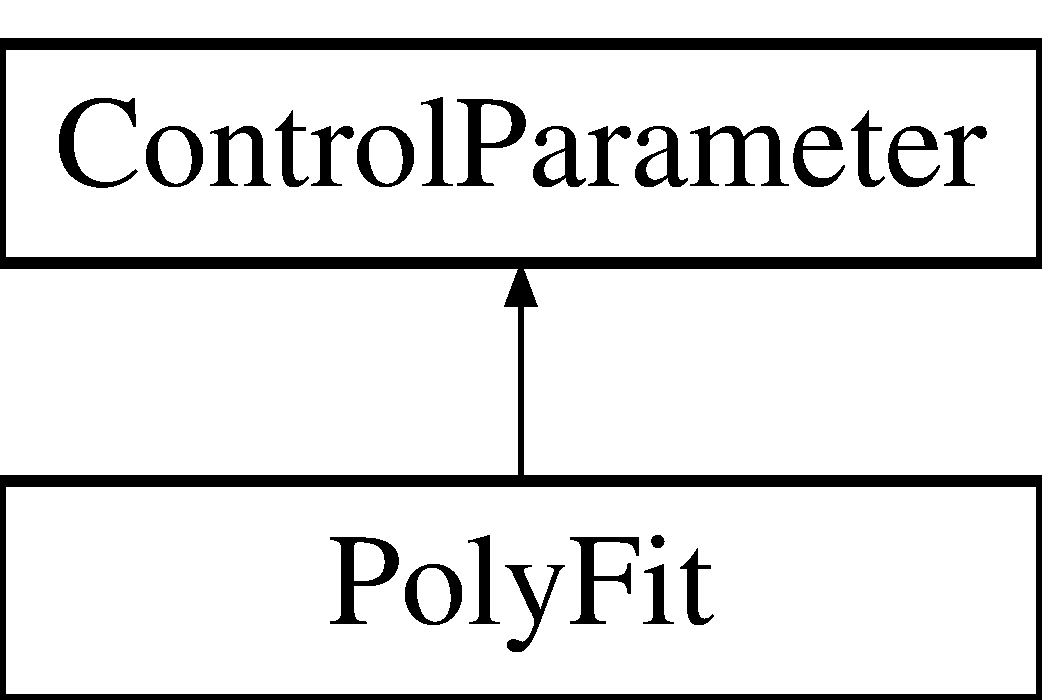
\includegraphics[height=2.000000cm]{class_poly_fit}
\end{center}
\end{figure}
\subsection*{Public Member Functions}
\begin{DoxyCompactItemize}
\item 
virtual \hyperlink{class_poly_fit_a3462736e02f02d3ab46ccd64aaf235d3}{$\sim$\-Poly\-Fit} ()
\item 
\hypertarget{class_poly_fit_a570b3d6805251459ef55904219726809}{double {\bfseries control\-Parameter} (\hyperlink{class_parameter_list}{Parameter\-List} \&min\-Par)}\label{class_poly_fit_a570b3d6805251459ef55904219726809}

\item 
\hypertarget{class_poly_fit_ad90dd471fea18051d5c0c2e5b483f0a5}{void {\bfseries draw\-Graph} (double a, double b, double c, double d)}\label{class_poly_fit_ad90dd471fea18051d5c0c2e5b483f0a5}

\end{DoxyCompactItemize}
\subsection*{Static Public Member Functions}
\begin{DoxyCompactItemize}
\item 
\hypertarget{class_poly_fit_a9a45808e526e84a5a8af50ff055d0c80}{static std\-::shared\-\_\-ptr\\*
$<$ \hyperlink{class_control_parameter}{Control\-Parameter} $>$ {\bfseries create\-Instance} (double p0, double p1, double p2, double p3, double sigma)}\label{class_poly_fit_a9a45808e526e84a5a8af50ff055d0c80}

\end{DoxyCompactItemize}
\subsection*{Additional Inherited Members}


\subsection{Detailed Description}
Test implementation of \hyperlink{class_control_parameter}{Control\-Parameter}. 

\subsection{Constructor \& Destructor Documentation}
\hypertarget{class_poly_fit_a3462736e02f02d3ab46ccd64aaf235d3}{\index{Poly\-Fit@{Poly\-Fit}!$\sim$\-Poly\-Fit@{$\sim$\-Poly\-Fit}}
\index{$\sim$\-Poly\-Fit@{$\sim$\-Poly\-Fit}!PolyFit@{Poly\-Fit}}
\subsubsection[{$\sim$\-Poly\-Fit}]{\setlength{\rightskip}{0pt plus 5cm}Poly\-Fit\-::$\sim$\-Poly\-Fit (
\begin{DoxyParamCaption}
{}
\end{DoxyParamCaption}
)\hspace{0.3cm}{\ttfamily [virtual]}}}\label{class_poly_fit_a3462736e02f02d3ab46ccd64aaf235d3}
Destructor 

The documentation for this class was generated from the following files\-:\begin{DoxyCompactItemize}
\item 
test/\hyperlink{_poly_fit_8hpp}{Poly\-Fit.\-hpp}\item 
test/Poly\-Fit.\-cpp\end{DoxyCompactItemize}

\hypertarget{struct_resonance}{\section{Resonance Struct Reference}
\label{struct_resonance}\index{Resonance@{Resonance}}
}
\subsection*{Data Fields}
\begin{DoxyCompactItemize}
\item 
\hypertarget{struct_resonance_a1f8a5834b734d5666dddd144ec8398bc}{std\-::string {\bfseries m\-\_\-name}}\label{struct_resonance_a1f8a5834b734d5666dddd144ec8398bc}

\item 
\hypertarget{struct_resonance_a8990beafbe0fcae02add43d56fbf76c2}{std\-::string {\bfseries m\-\_\-type}}\label{struct_resonance_a8990beafbe0fcae02add43d56fbf76c2}

\item 
\hypertarget{struct_resonance_acbe03f1359a0eb1bf721fea9a7a03b13}{std\-::string {\bfseries m\-\_\-reference}}\label{struct_resonance_acbe03f1359a0eb1bf721fea9a7a03b13}

\item 
\hypertarget{struct_resonance_ab9de5ccd6d828375f6619356f188bdbf}{double {\bfseries m\-\_\-mass}}\label{struct_resonance_ab9de5ccd6d828375f6619356f188bdbf}

\item 
\hypertarget{struct_resonance_ae58216b62a7b73ee275c228dc168d8e6}{double {\bfseries m\-\_\-mass\-\_\-min}}\label{struct_resonance_ae58216b62a7b73ee275c228dc168d8e6}

\item 
\hypertarget{struct_resonance_a10b762dd6be3a75ef2dbc7db8ce0df82}{double {\bfseries m\-\_\-mass\-\_\-max}}\label{struct_resonance_a10b762dd6be3a75ef2dbc7db8ce0df82}

\item 
\hypertarget{struct_resonance_ac429a425cd63073c04f3ed783df31a46}{double {\bfseries m\-\_\-breakup\-\_\-mom}}\label{struct_resonance_ac429a425cd63073c04f3ed783df31a46}

\item 
\hypertarget{struct_resonance_a6a164223523da9b82f05dfe412bf7d85}{double {\bfseries m\-\_\-width}}\label{struct_resonance_a6a164223523da9b82f05dfe412bf7d85}

\item 
\hypertarget{struct_resonance_a96cd124336b15b78a2da80667f754c16}{double {\bfseries m\-\_\-width\-\_\-min}}\label{struct_resonance_a96cd124336b15b78a2da80667f754c16}

\item 
\hypertarget{struct_resonance_aae6f37d58ee8ea168b28fff6db5065ff}{double {\bfseries m\-\_\-width\-\_\-max}}\label{struct_resonance_aae6f37d58ee8ea168b28fff6db5065ff}

\item 
\hypertarget{struct_resonance_a27cb65818c601155ee1641cfc69d9083}{double {\bfseries m\-\_\-par1}}\label{struct_resonance_a27cb65818c601155ee1641cfc69d9083}

\item 
\hypertarget{struct_resonance_aaba127e953445911c9ffc289fd5722e4}{double {\bfseries m\-\_\-par2}}\label{struct_resonance_aaba127e953445911c9ffc289fd5722e4}

\item 
\hypertarget{struct_resonance_a924fdc23c262d0536bb1c0aafcf167d9}{double {\bfseries m\-\_\-strength}}\label{struct_resonance_a924fdc23c262d0536bb1c0aafcf167d9}

\item 
\hypertarget{struct_resonance_a9979c547069b4a452c276a63da896a72}{double {\bfseries m\-\_\-phase}}\label{struct_resonance_a9979c547069b4a452c276a63da896a72}

\item 
\hypertarget{struct_resonance_a00abdd3572d15ba4474a1c31c1dc96ef}{unsigned int {\bfseries m\-\_\-spin}}\label{struct_resonance_a00abdd3572d15ba4474a1c31c1dc96ef}

\item 
\hypertarget{struct_resonance_ab9adb4ca4e03de9163a175be1c322685}{unsigned int {\bfseries m\-\_\-m}}\label{struct_resonance_ab9adb4ca4e03de9163a175be1c322685}

\item 
\hypertarget{struct_resonance_a6fddfde0c0200d51fd25496d17beb44d}{unsigned int {\bfseries m\-\_\-n}}\label{struct_resonance_a6fddfde0c0200d51fd25496d17beb44d}

\item 
\hypertarget{struct_resonance_a375c70fee829f4e5dd3a6ab9f266e7aa}{unsigned int {\bfseries m\-\_\-daugther\-A}}\label{struct_resonance_a375c70fee829f4e5dd3a6ab9f266e7aa}

\item 
\hypertarget{struct_resonance_ab5f5db09dd23c0e2bf1af0f8bcef96b2}{unsigned int {\bfseries m\-\_\-daugther\-B}}\label{struct_resonance_ab5f5db09dd23c0e2bf1af0f8bcef96b2}

\end{DoxyCompactItemize}


The documentation for this struct was generated from the following file\-:\begin{DoxyCompactItemize}
\item 
Physics/\-Amplitude\-Sum/\hyperlink{_amplitude_setup_8hpp}{Amplitude\-Setup.\-hpp}\end{DoxyCompactItemize}

\hypertarget{class_root_gen}{\section{Root\-Gen Class Reference}
\label{class_root_gen}\index{Root\-Gen@{Root\-Gen}}
}
\subsection*{Public Member Functions}
\begin{DoxyCompactItemize}
\item 
\hypertarget{class_root_gen_a03cddacd1835a9101c3e4ae7f02d7d8b}{{\bfseries Root\-Gen} (double in\-M, std\-::vector$<$ double $>$ fi\-M, std\-::vector$<$ int $>$ pids)}\label{class_root_gen_a03cddacd1835a9101c3e4ae7f02d7d8b}

\item 
\hypertarget{class_root_gen_ace2df560a26922a4daf848e9c2332cc7}{virtual void {\bfseries generate} (unsigned int n\-Events, std\-::shared\-\_\-pointer$<$ \hyperlink{class_amplitude}{Amplitude} $>$ model, std\-::string filename)}\label{class_root_gen_ace2df560a26922a4daf848e9c2332cc7}

\item 
\hypertarget{class_root_gen_a6c289aa8e2d6f8917e5baa1c74f9162c}{virtual void {\bfseries set\-Br} (const double in\-Br)}\label{class_root_gen_a6c289aa8e2d6f8917e5baa1c74f9162c}

\end{DoxyCompactItemize}


The documentation for this class was generated from the following files\-:\begin{DoxyCompactItemize}
\item 
Physics/\-Root\-Generator/\hyperlink{_root_gen_8hpp}{Root\-Gen.\-hpp}\item 
Physics/\-Root\-Generator/Root\-Gen.\-cpp\end{DoxyCompactItemize}

\hypertarget{class_root_reader}{\section{Root\-Reader Class Reference}
\label{class_root_reader}\index{Root\-Reader@{Root\-Reader}}
}


Reader for data in Root-\/files.  




{\ttfamily \#include $<$Root\-Reader.\-hpp$>$}

Inheritance diagram for Root\-Reader\-:\begin{figure}[H]
\begin{center}
\leavevmode
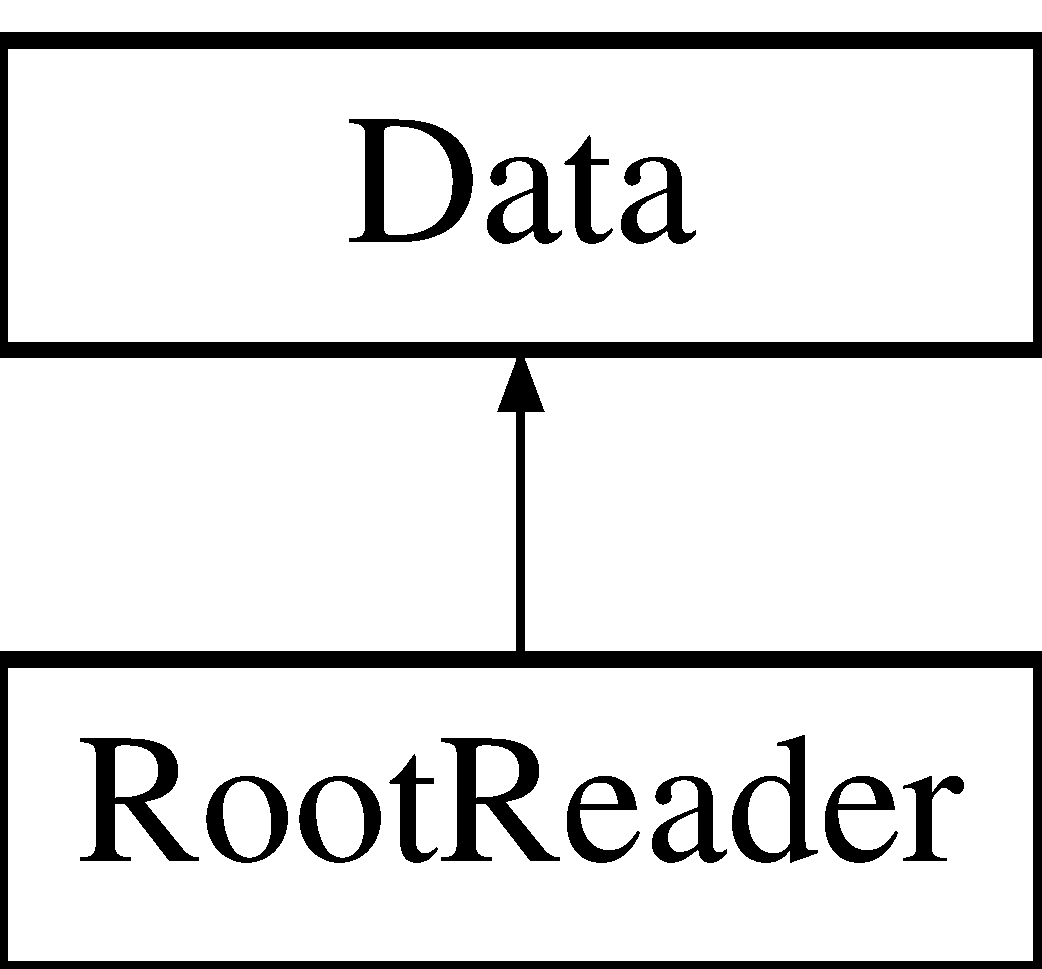
\includegraphics[height=2.000000cm]{class_root_reader}
\end{center}
\end{figure}
\subsection*{Public Member Functions}
\begin{DoxyCompactItemize}
\item 
\hypertarget{class_root_reader_a6f966c844aa3c2ac4fd3fe482586f827}{\hyperlink{class_root_reader_a6f966c844aa3c2ac4fd3fe482586f827}{Root\-Reader} ()}\label{class_root_reader_a6f966c844aa3c2ac4fd3fe482586f827}

\begin{DoxyCompactList}\small\item\em Default Constructor (0x0) \end{DoxyCompactList}\item 
\hypertarget{class_root_reader_af10d9979564e164fdd8085e3a7a8f473}{{\bfseries Root\-Reader} (const std\-::string in\-Root\-File, const bool binned, const std\-::string in\-Tree\-Name)}\label{class_root_reader_af10d9979564e164fdd8085e3a7a8f473}

\item 
\hypertarget{class_root_reader_a8fc5355f55d3f207ceca793df2ba3a07}{{\bfseries Root\-Reader} (T\-Tree $\ast$in, const bool binned)}\label{class_root_reader_a8fc5355f55d3f207ceca793df2ba3a07}

\item 
\hypertarget{class_root_reader_a1459a5bdb157ec3794c7f83c48456479}{virtual const std\-::vector\\*
$<$ std\-::string $>$ \& {\bfseries get\-Variable\-Names} ()}\label{class_root_reader_a1459a5bdb157ec3794c7f83c48456479}

\item 
\hypertarget{class_root_reader_a9abb0aca839119eaa81c07da411813cf}{virtual const \hyperlink{class_event}{Event} \& {\bfseries get\-Event} (const int)}\label{class_root_reader_a9abb0aca839119eaa81c07da411813cf}

\item 
\hypertarget{class_root_reader_ab4b78926472a13be4ae08e648fe70f15}{virtual const int {\bfseries get\-Bin} (const int, double \&, double \&)}\label{class_root_reader_ab4b78926472a13be4ae08e648fe70f15}

\item 
\hypertarget{class_root_reader_a035727b2548547a0c1b84bdf3799ab37}{virtual const unsigned int {\bfseries get\-N\-Events} () const }\label{class_root_reader_a035727b2548547a0c1b84bdf3799ab37}

\item 
\hypertarget{class_root_reader_a46c7618bb5376827c62e9c8e746a0cb2}{virtual const unsigned int {\bfseries get\-N\-Bins} () const }\label{class_root_reader_a46c7618bb5376827c62e9c8e746a0cb2}

\item 
virtual \hyperlink{class_root_reader_a926a707698e8f61dd3de1d2b329dd6a2}{$\sim$\-Root\-Reader} ()
\end{DoxyCompactItemize}
\subsection*{Protected Member Functions}
\begin{DoxyCompactItemize}
\item 
\hypertarget{class_root_reader_a4c2e6179e52197a407b5a5d216c48243}{virtual void {\bfseries store\-Events} ()}\label{class_root_reader_a4c2e6179e52197a407b5a5d216c48243}

\item 
\hypertarget{class_root_reader_a1cf7942febb7897b17baffe2c16a495e}{virtual void {\bfseries bin} ()}\label{class_root_reader_a1cf7942febb7897b17baffe2c16a495e}

\end{DoxyCompactItemize}
\subsection*{Protected Attributes}
\begin{DoxyCompactItemize}
\item 
\hypertarget{class_root_reader_a75af1a876b73e6833bdc6b254d65335b}{T\-File $\ast$ {\bfseries f\-File}}\label{class_root_reader_a75af1a876b73e6833bdc6b254d65335b}

\item 
\hypertarget{class_root_reader_ae3a20a6601087cecc748c4b50b94392f}{T\-Tree $\ast$ {\bfseries f\-Tree}}\label{class_root_reader_ae3a20a6601087cecc748c4b50b94392f}

\item 
\hypertarget{class_root_reader_a9c22fe9aa23f6c4299d534aad9b240ce}{T\-Clones\-Array $\ast$ {\bfseries f\-Particles}}\label{class_root_reader_a9c22fe9aa23f6c4299d534aad9b240ce}

\item 
\hypertarget{class_root_reader_a801a92cd6cd00322d0a89d5588132d10}{unsigned int {\bfseries fmax\-Events}}\label{class_root_reader_a801a92cd6cd00322d0a89d5588132d10}

\item 
\hypertarget{class_root_reader_a0e7cabbf6cd0878361886d76f48e5e79}{unsigned int {\bfseries f\-Event}}\label{class_root_reader_a0e7cabbf6cd0878361886d76f48e5e79}

\item 
\hypertarget{class_root_reader_a1b113b9995014a846c6096cb4e11eee2}{bool {\bfseries f\-Binned}}\label{class_root_reader_a1b113b9995014a846c6096cb4e11eee2}

\item 
\hypertarget{class_root_reader_a4dd8f02a657443032c57c90d07228aef}{unsigned int {\bfseries fmax\-Bins}}\label{class_root_reader_a4dd8f02a657443032c57c90d07228aef}

\item 
\hypertarget{class_root_reader_a46ba47478d9bcff794d0f6da72bd7173}{std\-::map$<$ int, std\-::pair\\*
$<$ double, double $>$ $>$ {\bfseries f\-Bins}}\label{class_root_reader_a46ba47478d9bcff794d0f6da72bd7173}

\item 
\hypertarget{class_root_reader_a2e494bd9033ff06a094069f69e885dcf}{std\-::vector$<$ std\-::string $>$ {\bfseries f\-Var\-Names}}\label{class_root_reader_a2e494bd9033ff06a094069f69e885dcf}

\item 
\hypertarget{class_root_reader_a4d54f4f3c26a75228e85af056f854994}{std\-::vector$<$ \hyperlink{class_event}{Event} $>$ {\bfseries f\-Events}}\label{class_root_reader_a4d54f4f3c26a75228e85af056f854994}

\end{DoxyCompactItemize}


\subsection{Detailed Description}
Reader for data in Root-\/files. 

\subsection{Constructor \& Destructor Documentation}
\hypertarget{class_root_reader_a926a707698e8f61dd3de1d2b329dd6a2}{\index{Root\-Reader@{Root\-Reader}!$\sim$\-Root\-Reader@{$\sim$\-Root\-Reader}}
\index{$\sim$\-Root\-Reader@{$\sim$\-Root\-Reader}!RootReader@{Root\-Reader}}
\subsubsection[{$\sim$\-Root\-Reader}]{\setlength{\rightskip}{0pt plus 5cm}Root\-Reader\-::$\sim$\-Root\-Reader (
\begin{DoxyParamCaption}
{}
\end{DoxyParamCaption}
)\hspace{0.3cm}{\ttfamily [virtual]}}}\label{class_root_reader_a926a707698e8f61dd3de1d2b329dd6a2}
Destructor 

The documentation for this class was generated from the following files\-:\begin{DoxyCompactItemize}
\item 
Data\-Reader/\-Root\-Reader/\hyperlink{_root_reader_8hpp}{Root\-Reader.\-hpp}\item 
Data\-Reader/\-Root\-Reader/Root\-Reader.\-cpp\end{DoxyCompactItemize}

\hypertarget{class_run_manager}{\section{Run\-Manager Class Reference}
\label{class_run_manager}\index{Run\-Manager@{Run\-Manager}}
}


Run-\/\-Manager for a simple fit.  




{\ttfamily \#include $<$Run\-Manager.\-hpp$>$}

\subsection*{Public Member Functions}
\begin{DoxyCompactItemize}
\item 
\hypertarget{class_run_manager_aead1ac6003c972f12a51560249624cef}{{\bfseries Run\-Manager} (std\-::shared\-\_\-ptr$<$ \hyperlink{class_data}{Data} $>$, std\-::shared\-\_\-ptr$<$ \hyperlink{class_control_parameter}{Control\-Parameter} $>$, std\-::shared\-\_\-ptr$<$ \hyperlink{class_amplitude}{Amplitude} $>$, std\-::shared\-\_\-ptr$<$ \hyperlink{class_optimizer}{Optimizer} $>$)}\label{class_run_manager_aead1ac6003c972f12a51560249624cef}

\item 
\hypertarget{class_run_manager_aede1e2e83985e2904b8b094d1b1eec12}{virtual bool {\bfseries start\-Fit} (\hyperlink{class_parameter_list}{Parameter\-List} \&)}\label{class_run_manager_aede1e2e83985e2904b8b094d1b1eec12}

\end{DoxyCompactItemize}
\subsection*{Protected Attributes}
\begin{DoxyCompactItemize}
\item 
std\-::shared\-\_\-ptr$<$ \hyperlink{class_data}{Data} $>$ \hyperlink{class_run_manager_ac5567c21ce343a46afb025643aa7add0}{p\-Data\-\_\-}
\item 
std\-::shared\-\_\-ptr$<$ \hyperlink{class_control_parameter}{Control\-Parameter} $>$ \hyperlink{class_run_manager_a37ed02a3d6f47131ef7e52a20816d48a}{p\-Esti\-\_\-}
\item 
std\-::shared\-\_\-ptr$<$ \hyperlink{class_amplitude}{Amplitude} $>$ \hyperlink{class_run_manager_a27ed6052f42c745bed63626b65f8dc77}{p\-Phys\-\_\-}
\item 
std\-::shared\-\_\-ptr$<$ \hyperlink{class_optimizer}{Optimizer} $>$ \hyperlink{class_run_manager_a55757983ceeeb8b4d687123e9804f6fc}{p\-Opti\-\_\-}
\item 
bool \hyperlink{class_run_manager_a0680769857728209363f2404a50a9f50}{valid\-\_\-}
\item 
bool \hyperlink{class_run_manager_a5d27906c077b0e898abd56722a593886}{success\-\_\-}
\end{DoxyCompactItemize}


\subsection{Detailed Description}
Run-\/\-Manager for a simple fit. 

\subsection{Field Documentation}
\hypertarget{class_run_manager_ac5567c21ce343a46afb025643aa7add0}{\index{Run\-Manager@{Run\-Manager}!p\-Data\-\_\-@{p\-Data\-\_\-}}
\index{p\-Data\-\_\-@{p\-Data\-\_\-}!RunManager@{Run\-Manager}}
\subsubsection[{p\-Data\-\_\-}]{\setlength{\rightskip}{0pt plus 5cm}std\-::shared\-\_\-ptr$<${\bf Data}$>$ Run\-Manager\-::p\-Data\-\_\-\hspace{0.3cm}{\ttfamily [protected]}}}\label{class_run_manager_ac5567c21ce343a46afb025643aa7add0}
Pointer to Data-\/\-Module \hypertarget{class_run_manager_a37ed02a3d6f47131ef7e52a20816d48a}{\index{Run\-Manager@{Run\-Manager}!p\-Esti\-\_\-@{p\-Esti\-\_\-}}
\index{p\-Esti\-\_\-@{p\-Esti\-\_\-}!RunManager@{Run\-Manager}}
\subsubsection[{p\-Esti\-\_\-}]{\setlength{\rightskip}{0pt plus 5cm}std\-::shared\-\_\-ptr$<${\bf Control\-Parameter}$>$ Run\-Manager\-::p\-Esti\-\_\-\hspace{0.3cm}{\ttfamily [protected]}}}\label{class_run_manager_a37ed02a3d6f47131ef7e52a20816d48a}
Pointer to Estimator-\/\-Module \hypertarget{class_run_manager_a55757983ceeeb8b4d687123e9804f6fc}{\index{Run\-Manager@{Run\-Manager}!p\-Opti\-\_\-@{p\-Opti\-\_\-}}
\index{p\-Opti\-\_\-@{p\-Opti\-\_\-}!RunManager@{Run\-Manager}}
\subsubsection[{p\-Opti\-\_\-}]{\setlength{\rightskip}{0pt plus 5cm}std\-::shared\-\_\-ptr$<${\bf Optimizer}$>$ Run\-Manager\-::p\-Opti\-\_\-\hspace{0.3cm}{\ttfamily [protected]}}}\label{class_run_manager_a55757983ceeeb8b4d687123e9804f6fc}
Pointer to Optimizer-\/\-Module \hypertarget{class_run_manager_a27ed6052f42c745bed63626b65f8dc77}{\index{Run\-Manager@{Run\-Manager}!p\-Phys\-\_\-@{p\-Phys\-\_\-}}
\index{p\-Phys\-\_\-@{p\-Phys\-\_\-}!RunManager@{Run\-Manager}}
\subsubsection[{p\-Phys\-\_\-}]{\setlength{\rightskip}{0pt plus 5cm}std\-::shared\-\_\-ptr$<${\bf Amplitude}$>$ Run\-Manager\-::p\-Phys\-\_\-\hspace{0.3cm}{\ttfamily [protected]}}}\label{class_run_manager_a27ed6052f42c745bed63626b65f8dc77}
Pointer to Physics-\/\-Module \hypertarget{class_run_manager_a5d27906c077b0e898abd56722a593886}{\index{Run\-Manager@{Run\-Manager}!success\-\_\-@{success\-\_\-}}
\index{success\-\_\-@{success\-\_\-}!RunManager@{Run\-Manager}}
\subsubsection[{success\-\_\-}]{\setlength{\rightskip}{0pt plus 5cm}bool Run\-Manager\-::success\-\_\-\hspace{0.3cm}{\ttfamily [protected]}}}\label{class_run_manager_a5d27906c077b0e898abd56722a593886}
fitting ended successfully? \hypertarget{class_run_manager_a0680769857728209363f2404a50a9f50}{\index{Run\-Manager@{Run\-Manager}!valid\-\_\-@{valid\-\_\-}}
\index{valid\-\_\-@{valid\-\_\-}!RunManager@{Run\-Manager}}
\subsubsection[{valid\-\_\-}]{\setlength{\rightskip}{0pt plus 5cm}bool Run\-Manager\-::valid\-\_\-\hspace{0.3cm}{\ttfamily [protected]}}}\label{class_run_manager_a0680769857728209363f2404a50a9f50}
setup a valid configuration? 

The documentation for this class was generated from the following files\-:\begin{DoxyCompactItemize}
\item 
Core/\hyperlink{_run_manager_8hpp}{Run\-Manager.\-hpp}\item 
Core/Run\-Manager.\-cpp\end{DoxyCompactItemize}

\hypertarget{class_slice_fit}{\section{Slice\-Fit Class Reference}
\label{class_slice_fit}\index{Slice\-Fit@{Slice\-Fit}}
}


\hyperlink{class_estimator}{Estimator} for a Fit of Dalitz-\/\-Plot Slices.  




{\ttfamily \#include $<$Slice\-Fit.\-hpp$>$}

Inheritance diagram for Slice\-Fit\-:\begin{figure}[H]
\begin{center}
\leavevmode
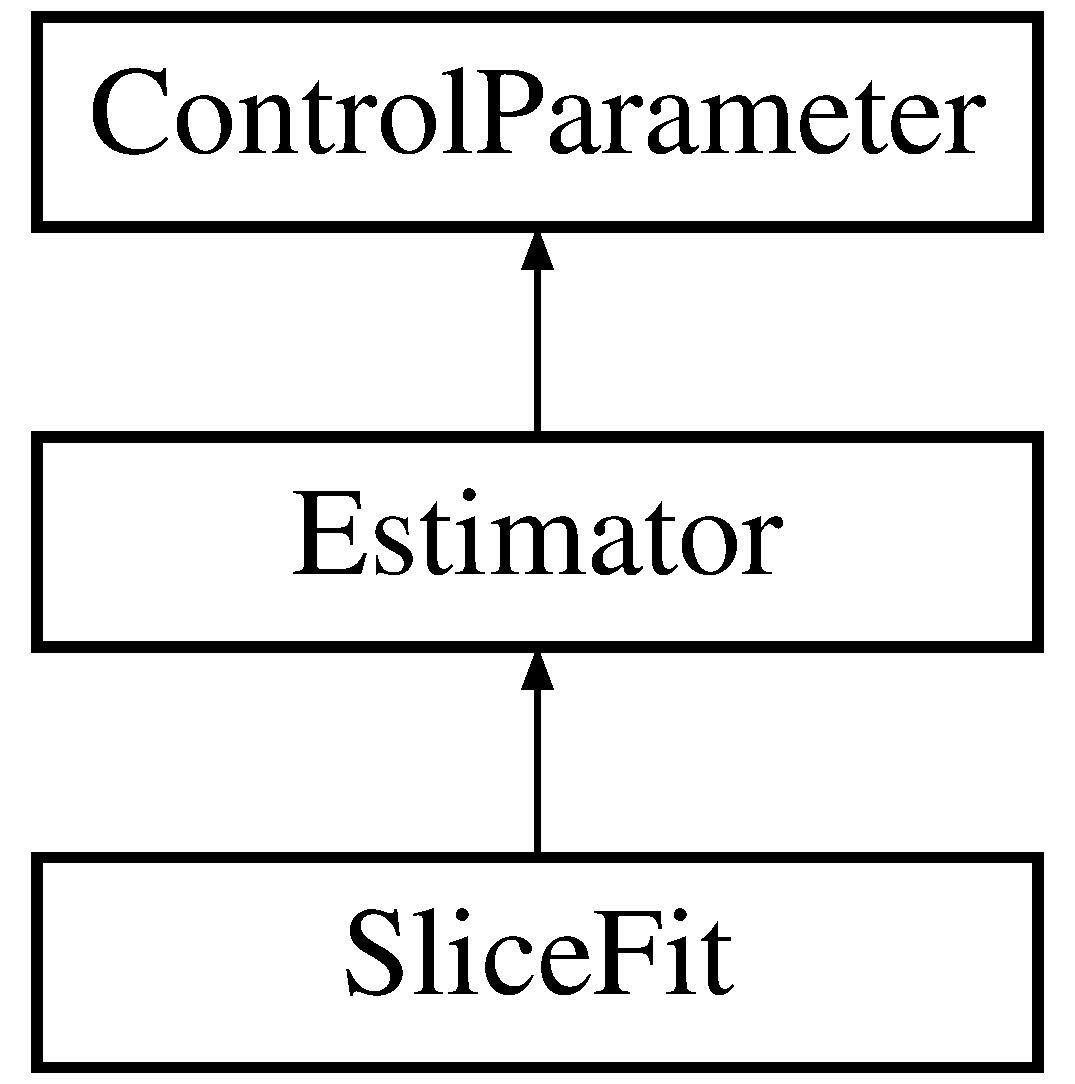
\includegraphics[height=3.000000cm]{class_slice_fit}
\end{center}
\end{figure}
\subsection*{Public Member Functions}
\begin{DoxyCompactItemize}
\item 
\hypertarget{class_slice_fit_abd46843e781866452d7587ad749d93d9}{\hyperlink{class_slice_fit_abd46843e781866452d7587ad749d93d9}{Slice\-Fit} (std\-::shared\-\_\-ptr$<$ \hyperlink{class_amplitude}{Amplitude} $>$, std\-::shared\-\_\-ptr$<$ \hyperlink{class_data}{Data} $>$)}\label{class_slice_fit_abd46843e781866452d7587ad749d93d9}

\begin{DoxyCompactList}\small\item\em Default Constructor (0x0) \end{DoxyCompactList}\item 
\hypertarget{class_slice_fit_a5fff370ea9a59ee149dba16c9e52e00d}{virtual double {\bfseries control\-Parameter} (\hyperlink{class_parameter_list}{Parameter\-List} \&min\-Par)}\label{class_slice_fit_a5fff370ea9a59ee149dba16c9e52e00d}

\item 
virtual \hyperlink{class_slice_fit_ab18be8542cbedb8c8c48b25badac3cb2}{$\sim$\-Slice\-Fit} ()
\end{DoxyCompactItemize}
\subsection*{Additional Inherited Members}


\subsection{Detailed Description}
\hyperlink{class_estimator}{Estimator} for a Fit of Dalitz-\/\-Plot Slices. 

\subsection{Constructor \& Destructor Documentation}
\hypertarget{class_slice_fit_ab18be8542cbedb8c8c48b25badac3cb2}{\index{Slice\-Fit@{Slice\-Fit}!$\sim$\-Slice\-Fit@{$\sim$\-Slice\-Fit}}
\index{$\sim$\-Slice\-Fit@{$\sim$\-Slice\-Fit}!SliceFit@{Slice\-Fit}}
\subsubsection[{$\sim$\-Slice\-Fit}]{\setlength{\rightskip}{0pt plus 5cm}Slice\-Fit\-::$\sim$\-Slice\-Fit (
\begin{DoxyParamCaption}
{}
\end{DoxyParamCaption}
)\hspace{0.3cm}{\ttfamily [virtual]}}}\label{class_slice_fit_ab18be8542cbedb8c8c48b25badac3cb2}
Destructor 

The documentation for this class was generated from the following files\-:\begin{DoxyCompactItemize}
\item 
Estimator/\-Slice\-Fit/\hyperlink{_slice_fit_8hpp}{Slice\-Fit.\-hpp}\item 
Estimator/\-Slice\-Fit/Slice\-Fit.\-cpp\end{DoxyCompactItemize}

\chapter{File Documentation}
\hypertarget{_dalitz_fit_app_8cpp}{\section{Analysis/\-Dalitz\-Fit\-App.cpp File Reference}
\label{_dalitz_fit_app_8cpp}\index{Analysis/\-Dalitz\-Fit\-App.\-cpp@{Analysis/\-Dalitz\-Fit\-App.\-cpp}}
}


Test-\/\-Application for full fit with simple B\-W-\/dalitz-\/model.  


{\ttfamily \#include $<$iostream$>$}\\*
{\ttfamily \#include $<$cmath$>$}\\*
{\ttfamily \#include $<$sstream$>$}\\*
{\ttfamily \#include $<$vector$>$}\\*
{\ttfamily \#include $<$string$>$}\\*
{\ttfamily \#include $<$memory$>$}\\*
{\ttfamily \#include \char`\"{}T\-F1.\-h\char`\"{}}\\*
{\ttfamily \#include \char`\"{}T\-H1\-D.\-h\char`\"{}}\\*
{\ttfamily \#include \char`\"{}T\-File.\-h\char`\"{}}\\*
{\ttfamily \#include \char`\"{}T\-Lorentz\-Vector.\-h\char`\"{}}\\*
{\ttfamily \#include \char`\"{}T\-H2\-D.\-h\char`\"{}}\\*
{\ttfamily \#include \char`\"{}Core/\-Event.\-hpp\char`\"{}}\\*
{\ttfamily \#include \char`\"{}Core/\-Particle.\-hpp\char`\"{}}\\*
{\ttfamily \#include \char`\"{}Core/\-Parameter.\-hpp\char`\"{}}\\*
{\ttfamily \#include \char`\"{}Core/\-Parameter\-List.\-hpp\char`\"{}}\\*
{\ttfamily \#include \char`\"{}Data\-Reader/\-Root\-Reader/\-Root\-Reader.\-hpp\char`\"{}}\\*
{\ttfamily \#include \char`\"{}Physics/\-Amplitude\-Sum/\-Amp\-Sum\-Intensity.\-hpp\char`\"{}}\\*
{\ttfamily \#include \char`\"{}Estimator/\-Min\-Log\-L\-H/\-Min\-Log\-L\-H.\-hpp\char`\"{}}\\*
{\ttfamily \#include \char`\"{}Optimizer/\-Minuit2/\-Minuit\-I\-F.\-hpp\char`\"{}}\\*
{\ttfamily \#include \char`\"{}Analysis/\-Plot\-Data.\-hpp\char`\"{}}\\*
\subsection*{Functions}
\begin{DoxyCompactItemize}
\item 
int \hyperlink{_dalitz_fit_app_8cpp_a3c04138a5bfe5d72780bb7e82a18e627}{main} (int argc, char $\ast$$\ast$argv)
\end{DoxyCompactItemize}
\subsection*{Variables}
\begin{DoxyCompactItemize}
\item 
\hypertarget{_dalitz_fit_app_8cpp_acb959f7b0abeddfde4175cb62025d56a}{const Double\-\_\-t {\bfseries M} = 3.\-096916}\label{_dalitz_fit_app_8cpp_acb959f7b0abeddfde4175cb62025d56a}

\item 
\hypertarget{_dalitz_fit_app_8cpp_a0a0f79bc350021411798f6ac6cfacbc7}{const Double\-\_\-t {\bfseries Br} = 0.\-000093}\label{_dalitz_fit_app_8cpp_a0a0f79bc350021411798f6ac6cfacbc7}

\item 
\hypertarget{_dalitz_fit_app_8cpp_ad4b1dc0c54e834c5c1ca325ebcd66fc3}{const Double\-\_\-t {\bfseries m1} = 0.}\label{_dalitz_fit_app_8cpp_ad4b1dc0c54e834c5c1ca325ebcd66fc3}

\item 
\hypertarget{_dalitz_fit_app_8cpp_ada5f2cdf434605648b802a0e13f67c82}{const Double\-\_\-t {\bfseries m2} = 0.\-139570}\label{_dalitz_fit_app_8cpp_ada5f2cdf434605648b802a0e13f67c82}

\item 
\hypertarget{_dalitz_fit_app_8cpp_ade198176253fe8f58cd46dae72aae18e}{const Double\-\_\-t {\bfseries m3} = 0.\-139570}\label{_dalitz_fit_app_8cpp_ade198176253fe8f58cd46dae72aae18e}

\item 
\hypertarget{_dalitz_fit_app_8cpp_ac410f6555ebc282703695e0831715846}{const Double\-\_\-t {\bfseries P\-I} = 3.\-14159}\label{_dalitz_fit_app_8cpp_ac410f6555ebc282703695e0831715846}

\end{DoxyCompactItemize}


\subsection{Detailed Description}
Test-\/\-Application for full fit with simple B\-W-\/dalitz-\/model. This tiny application tests a dalitz-\/fit procedure with a simple resonance model. It uses the simple L\-H-\/estimator \hyperlink{class_min_log_l_h}{Min\-Log\-L\-H}, it reads data via the root-\/reader module \hyperlink{class_root_reader}{Root\-Reader} and uses the intensity provided by the Breit-\/\-Wigner-\/\-Sum physics module Amplitude\-Sum. The optimization of the parameters is done with the Minuit2 module \hyperlink{class_minuit_i_f}{Minuit\-I\-F}. As result the optimized parameters are printed to the terminal. 

\subsection{Function Documentation}
\hypertarget{_dalitz_fit_app_8cpp_a3c04138a5bfe5d72780bb7e82a18e627}{\index{Dalitz\-Fit\-App.\-cpp@{Dalitz\-Fit\-App.\-cpp}!main@{main}}
\index{main@{main}!DalitzFitApp.cpp@{Dalitz\-Fit\-App.\-cpp}}
\subsubsection[{main}]{\setlength{\rightskip}{0pt plus 5cm}int main (
\begin{DoxyParamCaption}
\item[{int}]{argc, }
\item[{char $\ast$$\ast$}]{argv}
\end{DoxyParamCaption}
)}}\label{_dalitz_fit_app_8cpp_a3c04138a5bfe5d72780bb7e82a18e627}
The main function. 
\hypertarget{_dictionary_8hpp}{\section{Core/\-Dictionary.hpp File Reference}
\label{_dictionary_8hpp}\index{Core/\-Dictionary.\-hpp@{Core/\-Dictionary.\-hpp}}
}
{\ttfamily \#include $<$vector$>$}\\*
{\ttfamily \#include $<$map$>$}\\*
{\ttfamily \#include $<$memory$>$}\\*
{\ttfamily \#include $<$string$>$}\\*
{\ttfamily \#include \char`\"{}Core/\-Parameter.\-hpp\char`\"{}}\\*
{\ttfamily \#include \char`\"{}Core/\-Parameter\-List.\-hpp\char`\"{}}\\*
{\ttfamily \#include \char`\"{}Data\-Reader/\-Data.\-hpp\char`\"{}}\\*
{\ttfamily \#include \char`\"{}Physics/\-Amplitude.\-hpp\char`\"{}}\\*
\subsection*{Data Structures}
\begin{DoxyCompactItemize}
\item 
struct \hyperlink{structdata_info}{data\-Info}
\item 
struct \hyperlink{structamp_info}{amp\-Info}
\item 
class \hyperlink{class_dictionary}{Dictionary}
\begin{DoxyCompactList}\small\item\em \hyperlink{class_dictionary}{Dictionary} to manage information provided by modules. \end{DoxyCompactList}\end{DoxyCompactItemize}


\subsection{Detailed Description}
This class gathers information from modules, namely what they need as input and what they provide as output with the given input. 
\hypertarget{_event_8hpp}{\section{Core/\-Event.hpp File Reference}
\label{_event_8hpp}\index{Core/\-Event.\-hpp@{Core/\-Event.\-hpp}}
}
{\ttfamily \#include $<$vector$>$}\\*
{\ttfamily \#include \char`\"{}Core/\-Particle.\-hpp\char`\"{}}\\*
\subsection*{Data Structures}
\begin{DoxyCompactItemize}
\item 
class \hyperlink{class_event}{Event}
\begin{DoxyCompactList}\small\item\em Internal container for event information. \end{DoxyCompactList}\end{DoxyCompactItemize}


\subsection{Detailed Description}
This class provides a internal container for event-\/based information. The class provides a list of particles of the event. 
\hypertarget{_parameter_8hpp}{\section{Core/\-Parameter.hpp File Reference}
\label{_parameter_8hpp}\index{Core/\-Parameter.\-hpp@{Core/\-Parameter.\-hpp}}
}
{\ttfamily \#include $<$iostream$>$}\\*
{\ttfamily \#include $<$string$>$}\\*
{\ttfamily \#include $<$sstream$>$}\\*
{\ttfamily \#include \char`\"{}Core/\-Exceptions.\-hpp\char`\"{}}\\*
\subsection*{Data Structures}
\begin{DoxyCompactItemize}
\item 
class \hyperlink{class_double_parameter}{Double\-Parameter}
\begin{DoxyCompactList}\small\item\em Base class for internal parameter. \end{DoxyCompactList}\item 
class \hyperlink{class_integer_parameter}{Integer\-Parameter}
\item 
class \hyperlink{class_bool_parameter}{Bool\-Parameter}
\end{DoxyCompactItemize}
\subsection*{Functions}
\begin{DoxyCompactItemize}
\item 
std\-::ostream \& \hyperlink{_parameter_8hpp_a52a55b930010a730b7ff9415746f13a6}{operator$<$$<$} (std\-::ostream \&os, const \hyperlink{class_double_parameter}{Double\-Parameter} \&p)
\item 
std\-::ostream \& \hyperlink{_parameter_8hpp_ab9a320e078948aa0ce31b2adec766bfc}{operator$<$$<$} (std\-::ostream \&os, const \hyperlink{class_integer_parameter}{Integer\-Parameter} \&p)
\item 
std\-::ostream \& \hyperlink{_parameter_8hpp_a5239796d0d37d86b7003f4337efe920a}{operator$<$$<$} (std\-::ostream \&os, const \hyperlink{class_bool_parameter}{Bool\-Parameter} \&p)
\end{DoxyCompactItemize}


\subsection{Detailed Description}
This class defines the internal container of a fit parameter. A parameter consists of a value with optional bounds and error. 

\subsection{Function Documentation}
\hypertarget{_parameter_8hpp_a52a55b930010a730b7ff9415746f13a6}{\index{Parameter.\-hpp@{Parameter.\-hpp}!operator$<$$<$@{operator$<$$<$}}
\index{operator$<$$<$@{operator$<$$<$}!Parameter.hpp@{Parameter.\-hpp}}
\subsubsection[{operator$<$$<$}]{\setlength{\rightskip}{0pt plus 5cm}std\-::ostream\& operator$<$$<$ (
\begin{DoxyParamCaption}
\item[{std\-::ostream \&}]{os, }
\item[{const {\bf Double\-Parameter} \&}]{p}
\end{DoxyParamCaption}
)\hspace{0.3cm}{\ttfamily [inline]}}}\label{_parameter_8hpp_a52a55b930010a730b7ff9415746f13a6}
Declaring the stream-\/operator $<$$<$ as friend allows to stream parameter information to the output as easily as a generic type. The definition of this class has to be outside the namespace of the class. \begin{DoxySeeAlso}{See Also}
make\-\_\-str(), to\-\_\-str() 
\end{DoxySeeAlso}
\hypertarget{_parameter_8hpp_ab9a320e078948aa0ce31b2adec766bfc}{\index{Parameter.\-hpp@{Parameter.\-hpp}!operator$<$$<$@{operator$<$$<$}}
\index{operator$<$$<$@{operator$<$$<$}!Parameter.hpp@{Parameter.\-hpp}}
\subsubsection[{operator$<$$<$}]{\setlength{\rightskip}{0pt plus 5cm}std\-::ostream\& operator$<$$<$ (
\begin{DoxyParamCaption}
\item[{std\-::ostream \&}]{os, }
\item[{const {\bf Integer\-Parameter} \&}]{p}
\end{DoxyParamCaption}
)\hspace{0.3cm}{\ttfamily [inline]}}}\label{_parameter_8hpp_ab9a320e078948aa0ce31b2adec766bfc}
Declaring the stream-\/operator $<$$<$ as friend allows to stream parameter information to the output as easily as a generic type. The definition of this class has to be outside the namespace of the class. \begin{DoxySeeAlso}{See Also}
make\-\_\-str(), to\-\_\-str() 
\end{DoxySeeAlso}
\hypertarget{_parameter_8hpp_a5239796d0d37d86b7003f4337efe920a}{\index{Parameter.\-hpp@{Parameter.\-hpp}!operator$<$$<$@{operator$<$$<$}}
\index{operator$<$$<$@{operator$<$$<$}!Parameter.hpp@{Parameter.\-hpp}}
\subsubsection[{operator$<$$<$}]{\setlength{\rightskip}{0pt plus 5cm}std\-::ostream\& operator$<$$<$ (
\begin{DoxyParamCaption}
\item[{std\-::ostream \&}]{os, }
\item[{const {\bf Bool\-Parameter} \&}]{p}
\end{DoxyParamCaption}
)\hspace{0.3cm}{\ttfamily [inline]}}}\label{_parameter_8hpp_a5239796d0d37d86b7003f4337efe920a}
Declaring the stream-\/operator $<$$<$ as friend allows to stream parameter information to the output as easily as a generic type. The definition of this class has to be outside the namespace of the class. \begin{DoxySeeAlso}{See Also}
make\-\_\-str(), to\-\_\-str() 
\end{DoxySeeAlso}

\hypertarget{_parameter_list_8hpp}{\section{Core/\-Parameter\-List.hpp File Reference}
\label{_parameter_list_8hpp}\index{Core/\-Parameter\-List.\-hpp@{Core/\-Parameter\-List.\-hpp}}
}
{\ttfamily \#include $<$iostream$>$}\\*
{\ttfamily \#include $<$string$>$}\\*
{\ttfamily \#include $<$sstream$>$}\\*
{\ttfamily \#include $<$vector$>$}\\*
{\ttfamily \#include \char`\"{}Core/\-Parameter.\-hpp\char`\"{}}\\*
{\ttfamily \#include \char`\"{}Core/\-Exceptions.\-hpp\char`\"{}}\\*
\subsection*{Data Structures}
\begin{DoxyCompactItemize}
\item 
class \hyperlink{class_parameter_list}{Parameter\-List}
\begin{DoxyCompactList}\small\item\em Internal container representing a parameter list. \end{DoxyCompactList}\end{DoxyCompactItemize}


\subsection{Detailed Description}
This class provides a list of fit parameters which can have different types. It consists of a vectors of parameters of type double, int and bool. 
\hypertarget{_particle_8hpp}{\section{Core/\-Particle.hpp File Reference}
\label{_particle_8hpp}\index{Core/\-Particle.\-hpp@{Core/\-Particle.\-hpp}}
}
{\ttfamily \#include $<$vector$>$}\\*
{\ttfamily \#include $<$math.\-h$>$}\\*
\subsection*{Data Structures}
\begin{DoxyCompactItemize}
\item 
class \hyperlink{struct_particle}{Particle}
\begin{DoxyCompactList}\small\item\em Internal container representing a particle. \end{DoxyCompactList}\end{DoxyCompactItemize}


\subsection{Detailed Description}
This class provides a internal container for information of a particle. The class provides the momentum 4-\/vector and pid of the particle. 
\hypertarget{_run_manager_8hpp}{\section{Core/\-Run\-Manager.hpp File Reference}
\label{_run_manager_8hpp}\index{Core/\-Run\-Manager.\-hpp@{Core/\-Run\-Manager.\-hpp}}
}
{\ttfamily \#include $<$vector$>$}\\*
{\ttfamily \#include $<$memory$>$}\\*
{\ttfamily \#include \char`\"{}Data\-Reader/\-Data.\-hpp\char`\"{}}\\*
{\ttfamily \#include \char`\"{}Estimator/\-Estimator.\-hpp\char`\"{}}\\*
{\ttfamily \#include \char`\"{}Physics/\-Amplitude.\-hpp\char`\"{}}\\*
{\ttfamily \#include \char`\"{}Optimizer/\-Optimizer.\-hpp\char`\"{}}\\*
{\ttfamily \#include \char`\"{}Core/\-Parameter\-List.\-hpp\char`\"{}}\\*
\subsection*{Data Structures}
\begin{DoxyCompactItemize}
\item 
class \hyperlink{class_run_manager}{Run\-Manager}
\begin{DoxyCompactList}\small\item\em Run-\/\-Manager for a simple fit. \end{DoxyCompactList}\end{DoxyCompactItemize}


\subsection{Detailed Description}
This class provides a \hyperlink{class_run_manager}{Run\-Manager} for simple fits. To use it, you create all modules you want to use and provide them to the Run\-Manger. It checks for compatibility and if set up correctly it starts the fitting procedure. 
\hypertarget{_data_8hpp}{\section{Data\-Reader/\-Data.hpp File Reference}
\label{_data_8hpp}\index{Data\-Reader/\-Data.\-hpp@{Data\-Reader/\-Data.\-hpp}}
}
{\ttfamily \#include $<$vector$>$}\\*
{\ttfamily \#include $<$string$>$}\\*
{\ttfamily \#include \char`\"{}Core/\-Event.\-hpp\char`\"{}}\\*
\subsection*{Data Structures}
\begin{DoxyCompactItemize}
\item 
class \hyperlink{class_data}{Data}
\begin{DoxyCompactList}\small\item\em \hyperlink{class_data}{Data} Interface Base-\/\-Class. \end{DoxyCompactList}\end{DoxyCompactItemize}


\subsection{Detailed Description}
This class provides the interface to experimental data. As it is pure virtual, one needs at least one implementation to provide data for the other modules. If a new reader is derived from and fulfills this base-\/class, no change in other modules are necessary to work with the new dataset. 
\hypertarget{_root_reader_8hpp}{\section{Data\-Reader/\-Root\-Reader/\-Root\-Reader.hpp File Reference}
\label{_root_reader_8hpp}\index{Data\-Reader/\-Root\-Reader/\-Root\-Reader.\-hpp@{Data\-Reader/\-Root\-Reader/\-Root\-Reader.\-hpp}}
}
{\ttfamily \#include $<$vector$>$}\\*
{\ttfamily \#include $<$map$>$}\\*
{\ttfamily \#include $<$memory$>$}\\*
{\ttfamily \#include $<$string$>$}\\*
{\ttfamily \#include $<$utility$>$}\\*
{\ttfamily \#include \char`\"{}Data\-Reader/\-Data.\-hpp\char`\"{}}\\*
{\ttfamily \#include \char`\"{}Core/\-Event.\-hpp\char`\"{}}\\*
{\ttfamily \#include \char`\"{}T\-Math.\-h\char`\"{}}\\*
{\ttfamily \#include \char`\"{}T\-Lorentz\-Vector.\-h\char`\"{}}\\*
{\ttfamily \#include \char`\"{}T\-Particle.\-h\char`\"{}}\\*
{\ttfamily \#include \char`\"{}T\-R\-O\-O\-T.\-h\char`\"{}}\\*
{\ttfamily \#include \char`\"{}T\-File.\-h\char`\"{}}\\*
{\ttfamily \#include \char`\"{}T\-Clones\-Array.\-h\char`\"{}}\\*
{\ttfamily \#include \char`\"{}T\-Tree.\-h\char`\"{}}\\*
{\ttfamily \#include \char`\"{}T\-Random3.\-h\char`\"{}}\\*
\subsection*{Data Structures}
\begin{DoxyCompactItemize}
\item 
class \hyperlink{class_root_reader}{Root\-Reader}
\begin{DoxyCompactList}\small\item\em Reader for data in Root-\/files. \end{DoxyCompactList}\end{DoxyCompactItemize}


\subsection{Detailed Description}
This class reads event-\/based data from root-\/files. It implements the interface of \hyperlink{_data_8hpp}{Data.\-hpp}. 
\hypertarget{_chi_one_d_8hpp}{\section{Estimator/\-Chi\-One\-D/\-Chi\-One\-D.hpp File Reference}
\label{_chi_one_d_8hpp}\index{Estimator/\-Chi\-One\-D/\-Chi\-One\-D.\-hpp@{Estimator/\-Chi\-One\-D/\-Chi\-One\-D.\-hpp}}
}
{\ttfamily \#include $<$vector$>$}\\*
{\ttfamily \#include $<$memory$>$}\\*
{\ttfamily \#include $<$string$>$}\\*
{\ttfamily \#include \char`\"{}Estimator/\-Estimator.\-hpp\char`\"{}}\\*
{\ttfamily \#include \char`\"{}Physics/\-Amplitude.\-hpp\char`\"{}}\\*
{\ttfamily \#include \char`\"{}Data\-Reader/\-Data.\-hpp\char`\"{}}\\*
{\ttfamily \#include \char`\"{}Core/\-Event.\-hpp\char`\"{}}\\*
{\ttfamily \#include \char`\"{}Core/\-Parameter\-List.\-hpp\char`\"{}}\\*
\subsection*{Data Structures}
\begin{DoxyCompactItemize}
\item 
class \hyperlink{class_chi_one_d}{Chi\-One\-D}
\begin{DoxyCompactList}\small\item\em Simple $\chi^{2}$-\/\-Estimator. \end{DoxyCompactList}\end{DoxyCompactItemize}


\subsection{Detailed Description}
This class calculates a simple $\chi^{2}$ of a intensity and a dataset. \hyperlink{class_data}{Data} and Model are provided in the constructor using the \hyperlink{class_amplitude}{Amplitude} and \hyperlink{class_data}{Data} interfaces. The class itself fulfills the \hyperlink{class_estimator}{Estimator} interface. 
\hypertarget{_estimator_8hpp}{\section{Estimator/\-Estimator.hpp File Reference}
\label{_estimator_8hpp}\index{Estimator/\-Estimator.\-hpp@{Estimator/\-Estimator.\-hpp}}
}
{\ttfamily \#include $<$vector$>$}\\*
{\ttfamily \#include $<$memory$>$}\\*
{\ttfamily \#include \char`\"{}Optimizer/\-Control\-Parameter.\-hpp\char`\"{}}\\*
{\ttfamily \#include \char`\"{}Core/\-Parameter\-List.\-hpp\char`\"{}}\\*
\subsection*{Data Structures}
\begin{DoxyCompactItemize}
\item 
class \hyperlink{class_estimator}{Estimator}
\begin{DoxyCompactList}\small\item\em \hyperlink{class_estimator}{Estimator} Interface Base-\/\-Class. \end{DoxyCompactList}\end{DoxyCompactItemize}


\subsection{Detailed Description}
This class provides the interface to classes which estimate the \char`\"{}closeness\char`\"{} of the modeled intensity to the data. As it is pure virtual, one needs at least one implementation to provide an estimator for the analysis. If a new estimator is derived from and fulfills this base-\/class, no change in other modules are necessary to work with the new estimation function. As it is derived from \hyperlink{class_control_parameter}{Control\-Parameter}, it can be used in the optimizer modules. 
\hypertarget{_min_log_l_h_8hpp}{\section{Estimator/\-Min\-Log\-L\-H/\-Min\-Log\-L\-H.hpp File Reference}
\label{_min_log_l_h_8hpp}\index{Estimator/\-Min\-Log\-L\-H/\-Min\-Log\-L\-H.\-hpp@{Estimator/\-Min\-Log\-L\-H/\-Min\-Log\-L\-H.\-hpp}}
}
{\ttfamily \#include $<$vector$>$}\\*
{\ttfamily \#include $<$memory$>$}\\*
{\ttfamily \#include $<$string$>$}\\*
{\ttfamily \#include \char`\"{}Estimator/\-Estimator.\-hpp\char`\"{}}\\*
{\ttfamily \#include \char`\"{}Physics/\-Amplitude.\-hpp\char`\"{}}\\*
{\ttfamily \#include \char`\"{}Data\-Reader/\-Data.\-hpp\char`\"{}}\\*
{\ttfamily \#include \char`\"{}Core/\-Event.\-hpp\char`\"{}}\\*
{\ttfamily \#include \char`\"{}Core/\-Parameter\-List.\-hpp\char`\"{}}\\*
\subsection*{Data Structures}
\begin{DoxyCompactItemize}
\item 
class \hyperlink{class_min_log_l_h}{Min\-Log\-L\-H}
\end{DoxyCompactItemize}


\subsection{Detailed Description}
This class calculates a simple -\/log(L\-H) of a intensity and a dataset. \hyperlink{class_data}{Data} and Model are provided in the constructor using the \hyperlink{class_amplitude}{Amplitude} and \hyperlink{class_data}{Data} interfaces. The class itself fulfills the \hyperlink{class_estimator}{Estimator} interface. 
\hypertarget{_slice_fit_8hpp}{\section{Estimator/\-Slice\-Fit/\-Slice\-Fit.hpp File Reference}
\label{_slice_fit_8hpp}\index{Estimator/\-Slice\-Fit/\-Slice\-Fit.\-hpp@{Estimator/\-Slice\-Fit/\-Slice\-Fit.\-hpp}}
}
{\ttfamily \#include $<$vector$>$}\\*
{\ttfamily \#include $<$memory$>$}\\*
{\ttfamily \#include $<$string$>$}\\*
{\ttfamily \#include \char`\"{}T\-H2\-D.\-h\char`\"{}}\\*
{\ttfamily \#include \char`\"{}T\-Graph.\-h\char`\"{}}\\*
{\ttfamily \#include \char`\"{}T\-Graph\-Errors.\-h\char`\"{}}\\*
{\ttfamily \#include \char`\"{}T\-F1.\-h\char`\"{}}\\*
{\ttfamily \#include \char`\"{}Estimator/\-Estimator.\-hpp\char`\"{}}\\*
{\ttfamily \#include \char`\"{}Physics/\-Amplitude.\-hpp\char`\"{}}\\*
{\ttfamily \#include \char`\"{}Data\-Reader/\-Data.\-hpp\char`\"{}}\\*
{\ttfamily \#include \char`\"{}Core/\-Event.\-hpp\char`\"{}}\\*
{\ttfamily \#include \char`\"{}Core/\-Parameter\-List.\-hpp\char`\"{}}\\*
\subsection*{Data Structures}
\begin{DoxyCompactItemize}
\item 
class \hyperlink{class_slice_fit}{Slice\-Fit}
\begin{DoxyCompactList}\small\item\em \hyperlink{class_estimator}{Estimator} for a Fit of Dalitz-\/\-Plot Slices. \end{DoxyCompactList}\end{DoxyCompactItemize}


\subsection{Detailed Description}
This class performs a Chi2-\/\-Fit on slices along one axis of a dalitz-\/plot. The Dalitz-\/\-Plot is generated directly in the constructor of this \hyperlink{class_estimator}{Estimator}. \hyperlink{class_data}{Data} and Model are provided in the constructor using the \hyperlink{class_amplitude}{Amplitude} and \hyperlink{class_data}{Data} interfaces. The class itself fulfills the \hyperlink{class_estimator}{Estimator} interface. 
\hypertarget{_control_parameter_8hpp}{\section{Optimizer/\-Control\-Parameter.hpp File Reference}
\label{_control_parameter_8hpp}\index{Optimizer/\-Control\-Parameter.\-hpp@{Optimizer/\-Control\-Parameter.\-hpp}}
}
{\ttfamily \#include $<$vector$>$}\\*
{\ttfamily \#include $<$memory$>$}\\*
{\ttfamily \#include \char`\"{}Core/\-Parameter\-List.\-hpp\char`\"{}}\\*
\subsection*{Data Structures}
\begin{DoxyCompactItemize}
\item 
class \hyperlink{class_control_parameter}{Control\-Parameter}
\begin{DoxyCompactList}\small\item\em \hyperlink{class_optimizer}{Optimizer} \hyperlink{class_data}{Data} Base-\/\-Class. \end{DoxyCompactList}\end{DoxyCompactItemize}


\subsection{Detailed Description}
This class provides the interface for the optimizer module to access the data. If the access to the data is provided fulfilling this interface, then one can use the same data and parameter-\/set with different optimizers. 
\hypertarget{_geneva_i_f_8hpp}{\section{Optimizer/\-Geneva/\-Geneva\-I\-F.hpp File Reference}
\label{_geneva_i_f_8hpp}\index{Optimizer/\-Geneva/\-Geneva\-I\-F.\-hpp@{Optimizer/\-Geneva/\-Geneva\-I\-F.\-hpp}}
}
{\ttfamily \#include $<$vector$>$}\\*
{\ttfamily \#include $<$memory$>$}\\*
{\ttfamily \#include $<$iostream$>$}\\*
{\ttfamily \#include \char`\"{}Optimizer/\-Control\-Parameter.\-hpp\char`\"{}}\\*
{\ttfamily \#include \char`\"{}Optimizer/\-Optimizer.\-hpp\char`\"{}}\\*
{\ttfamily \#include \char`\"{}Core/\-Parameter\-List.\-hpp\char`\"{}}\\*
{\ttfamily \#include \char`\"{}Core/\-Parameter.\-hpp\char`\"{}}\\*
{\ttfamily \#include \char`\"{}Optimizer/\-Geneva/\-G\-Start\-Individual.\-hpp\char`\"{}}\\*
{\ttfamily \#include $<$boost/program\-\_\-options.\-hpp$>$}\\*
{\ttfamily \#include $<$boost/filesystem.\-hpp$>$}\\*
{\ttfamily \#include \char`\"{}geneva/\-Go2.\-hpp\char`\"{}}\\*
\subsection*{Data Structures}
\begin{DoxyCompactItemize}
\item 
class \hyperlink{class_geneva_i_f}{Geneva\-I\-F}
\begin{DoxyCompactList}\small\item\em Wrapper of the Geneva \hyperlink{class_optimizer}{Optimizer} library. \end{DoxyCompactList}\end{DoxyCompactItemize}


\subsection{Detailed Description}
This class provides a wrapper around the Geneva library. It fulfills the \hyperlink{class_optimizer}{Optimizer} interface to be easily adapted to other modules. Parameters for the optimization have to be provided in a config-\/file, the data needs to be provided with the \hyperlink{class_control_parameter}{Control\-Parameter} interface. 
\hypertarget{_g_start_individual_8hpp}{\section{Optimizer/\-Geneva/\-G\-Start\-Individual.hpp File Reference}
\label{_g_start_individual_8hpp}\index{Optimizer/\-Geneva/\-G\-Start\-Individual.\-hpp@{Optimizer/\-Geneva/\-G\-Start\-Individual.\-hpp}}
}
{\ttfamily \#include $<$iostream$>$}\\*
{\ttfamily \#include $<$common/\-G\-Global\-Defines.\-hpp$>$}\\*
{\ttfamily \#include $<$boost/shared\-\_\-ptr.\-hpp$>$}\\*
{\ttfamily \#include $<$Core/\-Parameter\-List.\-hpp$>$}\\*
{\ttfamily \#include $<$Optimizer/\-Control\-Parameter.\-hpp$>$}\\*
{\ttfamily \#include $<$geneva/\-G\-Parameter\-Set.\-hpp$>$}\\*
{\ttfamily \#include $<$geneva/\-G\-Constrained\-Double\-Object.\-hpp$>$}\\*
\subsection*{Data Structures}
\begin{DoxyCompactItemize}
\item 
class \hyperlink{class_gem_1_1_geneva_1_1_g_start_individual}{Gem\-::\-Geneva\-::\-G\-Start\-Individual}
\end{DoxyCompactItemize}

\hypertarget{_minuit_fcn_8hpp}{\section{Optimizer/\-Minuit2/\-Minuit\-Fcn.hpp File Reference}
\label{_minuit_fcn_8hpp}\index{Optimizer/\-Minuit2/\-Minuit\-Fcn.\-hpp@{Optimizer/\-Minuit2/\-Minuit\-Fcn.\-hpp}}
}
{\ttfamily \#include $<$vector$>$}\\*
{\ttfamily \#include $<$memory$>$}\\*
{\ttfamily \#include \char`\"{}Minuit2/\-F\-C\-N\-Base.\-h\char`\"{}}\\*
{\ttfamily \#include \char`\"{}Optimizer/\-Control\-Parameter.\-hpp\char`\"{}}\\*
{\ttfamily \#include \char`\"{}Core/\-Parameter\-List.\-hpp\char`\"{}}\\*
\subsection*{Data Structures}
\begin{DoxyCompactItemize}
\item 
class \hyperlink{class_r_o_o_t_1_1_minuit2_1_1_minuit_fcn}{R\-O\-O\-T\-::\-Minuit2\-::\-Minuit\-Fcn}
\end{DoxyCompactItemize}


\subsection{Detailed Description}
Based on the Minuit2 Fcn\-Base. This class uses the \hyperlink{class_control_parameter}{Control\-Parameter} interface for the optimization. 
\hypertarget{_minuit_i_f_8hpp}{\section{Optimizer/\-Minuit2/\-Minuit\-I\-F.hpp File Reference}
\label{_minuit_i_f_8hpp}\index{Optimizer/\-Minuit2/\-Minuit\-I\-F.\-hpp@{Optimizer/\-Minuit2/\-Minuit\-I\-F.\-hpp}}
}
{\ttfamily \#include $<$vector$>$}\\*
{\ttfamily \#include $<$memory$>$}\\*
{\ttfamily \#include \char`\"{}Optimizer/\-Control\-Parameter.\-hpp\char`\"{}}\\*
{\ttfamily \#include \char`\"{}Optimizer/\-Optimizer.\-hpp\char`\"{}}\\*
{\ttfamily \#include \char`\"{}Core/\-Parameter\-List.\-hpp\char`\"{}}\\*
{\ttfamily \#include \char`\"{}Optimizer/\-Minuit2/\-Minuit\-Fcn.\-hpp\char`\"{}}\\*
\subsection*{Data Structures}
\begin{DoxyCompactItemize}
\item 
class \hyperlink{class_minuit_i_f}{Minuit\-I\-F}
\begin{DoxyCompactList}\small\item\em Wrapper of the Minuit2 \hyperlink{class_optimizer}{Optimizer} library. \end{DoxyCompactList}\end{DoxyCompactItemize}


\subsection{Detailed Description}
This class provides a wrapper around the Minuit2 library. It fulfills the \hyperlink{class_optimizer}{Optimizer} interface to be easily adapted to other modules. The data needs to be provided with the \hyperlink{class_control_parameter}{Control\-Parameter} interface. 
\hypertarget{_optimizer_8hpp}{\section{Optimizer/\-Optimizer.hpp File Reference}
\label{_optimizer_8hpp}\index{Optimizer/\-Optimizer.\-hpp@{Optimizer/\-Optimizer.\-hpp}}
}
{\ttfamily \#include $<$vector$>$}\\*
{\ttfamily \#include $<$memory$>$}\\*
{\ttfamily \#include \char`\"{}Core/\-Parameter\-List.\-hpp\char`\"{}}\\*
\subsection*{Data Structures}
\begin{DoxyCompactItemize}
\item 
class \hyperlink{class_optimizer}{Optimizer}
\begin{DoxyCompactList}\small\item\em \hyperlink{class_optimizer}{Optimizer} Interface Base-\/\-Class. \end{DoxyCompactList}\end{DoxyCompactItemize}


\subsection{Detailed Description}
This class provides the interface to (external) optimization libraries or routines. As it is pure virtual, one needs at least one implementation to provide an optimizer for the analysis which varies free model-\/parameters. If a new optimizer is derived from and fulfills this base-\/class, no change in other modules are necessary to work with the new optimizer library or routine. 
\hypertarget{_amplitude_8hpp}{\section{Physics/\-Amplitude.hpp File Reference}
\label{_amplitude_8hpp}\index{Physics/\-Amplitude.\-hpp@{Physics/\-Amplitude.\-hpp}}
}
{\ttfamily \#include $<$vector$>$}\\*
{\ttfamily \#include $<$memory$>$}\\*
{\ttfamily \#include \char`\"{}Core/\-Parameter\-List.\-hpp\char`\"{}}\\*
\subsection*{Data Structures}
\begin{DoxyCompactItemize}
\item 
class \hyperlink{class_amplitude}{Amplitude}
\begin{DoxyCompactList}\small\item\em Physics Interface Base-\/\-Class. \end{DoxyCompactList}\end{DoxyCompactItemize}


\subsection{Detailed Description}
This class provides the interface to the model which tries to describe the intensity. As it is pure virtual, one needs at least one implementation to provide an model for the analysis which calculates intensities for an event on basis model parameters. If a new physics-\/model is derived from and fulfills this base-\/class, no change in other modules are necessary to work with the new physics module. 
\hypertarget{_amplitude_setup_8hpp}{\section{Physics/\-Amplitude\-Sum/\-Amplitude\-Setup.hpp File Reference}
\label{_amplitude_setup_8hpp}\index{Physics/\-Amplitude\-Sum/\-Amplitude\-Setup.\-hpp@{Physics/\-Amplitude\-Sum/\-Amplitude\-Setup.\-hpp}}
}


X\-M\-L config parser for \hyperlink{class_amplitude}{Amplitude} Setup.  


{\ttfamily \#include $<$vector$>$}\\*
{\ttfamily \#include $<$string$>$}\\*
{\ttfamily \#include $<$memory$>$}\\*
{\ttfamily \#include $<$boost/foreach.\-hpp$>$}\\*
{\ttfamily \#include $<$boost/property\-\_\-tree/ptree.\-hpp$>$}\\*
{\ttfamily \#include $<$boost/property\-\_\-tree/xml\-\_\-parser.\-hpp$>$}\\*
\subsection*{Data Structures}
\begin{DoxyCompactItemize}
\item 
struct \hyperlink{struct_resonance}{Resonance}
\item 
class \hyperlink{class_amplitude_setup}{Amplitude\-Setup}
\end{DoxyCompactItemize}


\subsection{Detailed Description}
X\-M\-L config parser for \hyperlink{class_amplitude}{Amplitude} Setup. 
\hypertarget{_breit_wigner_8hpp}{\section{Physics/\-Breit\-Wigner/\-Breit\-Wigner.hpp File Reference}
\label{_breit_wigner_8hpp}\index{Physics/\-Breit\-Wigner/\-Breit\-Wigner.\-hpp@{Physics/\-Breit\-Wigner/\-Breit\-Wigner.\-hpp}}
}
{\ttfamily \#include $<$vector$>$}\\*
{\ttfamily \#include $<$memory$>$}\\*
{\ttfamily \#include \char`\"{}Physics/\-Amplitude.\-hpp\char`\"{}}\\*
{\ttfamily \#include \char`\"{}Core/\-Parameter\-List.\-hpp\char`\"{}}\\*
\subsection*{Data Structures}
\begin{DoxyCompactItemize}
\item 
class \hyperlink{class_breit_wigner}{Breit\-Wigner}
\begin{DoxyCompactList}\small\item\em Physics Module with simple 1\-D Breit-\/\-Wigner. \end{DoxyCompactList}\end{DoxyCompactItemize}


\subsection{Detailed Description}
This class provides a simple Breit-\/\-Wigner calculation with given parameters. It fulfills the \hyperlink{class_amplitude}{Amplitude} interface to be compatible with other Com\-P\-W\-A modules. 
\hypertarget{_root_gen_8hpp}{\section{Physics/\-Root\-Generator/\-Root\-Gen.hpp File Reference}
\label{_root_gen_8hpp}\index{Physics/\-Root\-Generator/\-Root\-Gen.\-hpp@{Physics/\-Root\-Generator/\-Root\-Gen.\-hpp}}
}


Class to generate 4-\/\-Vectors.  


{\ttfamily \#include $<$iostream$>$}\\*
{\ttfamily \#include $<$cmath$>$}\\*
{\ttfamily \#include $<$sstream$>$}\\*
{\ttfamily \#include $<$vector$>$}\\*
{\ttfamily \#include $<$string$>$}\\*
{\ttfamily \#include $<$memory$>$}\\*
{\ttfamily \#include \char`\"{}Physics/\-Amplitude.\-hpp\char`\"{}}\\*
{\ttfamily \#include \char`\"{}Core/\-P\-W\-A\-Parameter.\-hpp\char`\"{}}\\*
{\ttfamily \#include \char`\"{}Core/\-P\-W\-A\-Generic\-Par.\-hpp\char`\"{}}\\*
\subsection*{Data Structures}
\begin{DoxyCompactItemize}
\item 
class \hyperlink{class_root_gen}{Root\-Gen}
\end{DoxyCompactItemize}


\subsection{Detailed Description}
Class to generate 4-\/\-Vectors. This application uses arbitrary \hyperlink{class_amplitude}{Amplitude} implementations and the root phase-\/space generator to generate a root-\/file with 4-\/\-Vectors distributed according the given amplitude model. 
\hypertarget{_data_i_f_test_app_8cpp}{\section{test/\-Data\-I\-F\-Test\-App.cpp File Reference}
\label{_data_i_f_test_app_8cpp}\index{test/\-Data\-I\-F\-Test\-App.\-cpp@{test/\-Data\-I\-F\-Test\-App.\-cpp}}
}


Test-\/\-Application of the Root Data-\/\-I\-F.  


{\ttfamily \#include $<$iostream$>$}\\*
{\ttfamily \#include $<$cmath$>$}\\*
{\ttfamily \#include $<$sstream$>$}\\*
{\ttfamily \#include $<$vector$>$}\\*
{\ttfamily \#include $<$string$>$}\\*
{\ttfamily \#include $<$memory$>$}\\*
{\ttfamily \#include \char`\"{}T\-Lorentz\-Vector.\-h\char`\"{}}\\*
{\ttfamily \#include \char`\"{}T\-H1\-D.\-h\char`\"{}}\\*
{\ttfamily \#include \char`\"{}T\-File.\-h\char`\"{}}\\*
{\ttfamily \#include \char`\"{}Data\-Reader/\-Root\-Reader/\-Root\-Reader.\-hpp\char`\"{}}\\*
{\ttfamily \#include \char`\"{}Core/\-Event.\-hpp\char`\"{}}\\*
{\ttfamily \#include \char`\"{}Core/\-Particle.\-hpp\char`\"{}}\\*
\subsection*{Functions}
\begin{DoxyCompactItemize}
\item 
int \hyperlink{_data_i_f_test_app_8cpp_a3c04138a5bfe5d72780bb7e82a18e627}{main} (int argc, char $\ast$$\ast$argv)
\end{DoxyCompactItemize}


\subsection{Detailed Description}
Test-\/\-Application of the Root Data-\/\-I\-F. This tiny application tests the Root-\/format Data-\/\-I\-F. It reads a root file, plots the invariant mass of the first two particles and writes the result as well to another root file. 

\subsection{Function Documentation}
\hypertarget{_data_i_f_test_app_8cpp_a3c04138a5bfe5d72780bb7e82a18e627}{\index{Data\-I\-F\-Test\-App.\-cpp@{Data\-I\-F\-Test\-App.\-cpp}!main@{main}}
\index{main@{main}!DataIFTestApp.cpp@{Data\-I\-F\-Test\-App.\-cpp}}
\subsubsection[{main}]{\setlength{\rightskip}{0pt plus 5cm}int main (
\begin{DoxyParamCaption}
\item[{int}]{argc, }
\item[{char $\ast$$\ast$}]{argv}
\end{DoxyParamCaption}
)}}\label{_data_i_f_test_app_8cpp_a3c04138a5bfe5d72780bb7e82a18e627}
The main function. 
\hypertarget{_estimator_test_app_8cpp}{\section{test/\-Estimator\-Test\-App.cpp File Reference}
\label{_estimator_test_app_8cpp}\index{test/\-Estimator\-Test\-App.\-cpp@{test/\-Estimator\-Test\-App.\-cpp}}
}


Test-\/\-Application of a simple $\chi^{2}$ estimator.  


{\ttfamily \#include $<$iostream$>$}\\*
{\ttfamily \#include $<$cmath$>$}\\*
{\ttfamily \#include $<$sstream$>$}\\*
{\ttfamily \#include $<$vector$>$}\\*
{\ttfamily \#include $<$string$>$}\\*
{\ttfamily \#include $<$memory$>$}\\*
{\ttfamily \#include \char`\"{}Data\-Reader/\-Root\-Reader/\-Root\-Reader.\-hpp\char`\"{}}\\*
{\ttfamily \#include \char`\"{}Physics/\-Breit\-Wigner/\-Breit\-Wigner.\-hpp\char`\"{}}\\*
{\ttfamily \#include \char`\"{}Estimator/\-Min\-Log\-L\-H/\-Min\-Log\-L\-H.\-hpp\char`\"{}}\\*
{\ttfamily \#include \char`\"{}Estimator/\-Chi\-One\-D/\-Chi\-One\-D.\-hpp\char`\"{}}\\*
{\ttfamily \#include \char`\"{}Core/\-Particle.\-hpp\char`\"{}}\\*
{\ttfamily \#include \char`\"{}Core/\-Parameter.\-hpp\char`\"{}}\\*
{\ttfamily \#include \char`\"{}Core/\-Parameter\-List.\-hpp\char`\"{}}\\*
\subsection*{Functions}
\begin{DoxyCompactItemize}
\item 
int \hyperlink{_estimator_test_app_8cpp_a3c04138a5bfe5d72780bb7e82a18e627}{main} (int argc, char $\ast$$\ast$argv)
\end{DoxyCompactItemize}


\subsection{Detailed Description}
Test-\/\-Application of a simple $\chi^{2}$ estimator. This tiny application tests a simple $\chi^{2}$ estimator module. It reads data via the root-\/reader module \hyperlink{class_root_reader}{Root\-Reader},hpp and uses the intensity provided by the simple 1\-D-\/\-Breit-\/\-Wigner physics module \hyperlink{_breit_wigner_8hpp}{Breit\-Wigner.\-hpp}. As result it prints a calculated $\chi^{2}$ to the terminal. 

\subsection{Function Documentation}
\hypertarget{_estimator_test_app_8cpp_a3c04138a5bfe5d72780bb7e82a18e627}{\index{Estimator\-Test\-App.\-cpp@{Estimator\-Test\-App.\-cpp}!main@{main}}
\index{main@{main}!EstimatorTestApp.cpp@{Estimator\-Test\-App.\-cpp}}
\subsubsection[{main}]{\setlength{\rightskip}{0pt plus 5cm}int main (
\begin{DoxyParamCaption}
\item[{int}]{argc, }
\item[{char $\ast$$\ast$}]{argv}
\end{DoxyParamCaption}
)}}\label{_estimator_test_app_8cpp_a3c04138a5bfe5d72780bb7e82a18e627}
The main function. 
\hypertarget{_gen_two_part_app_8cpp}{\section{test/\-Gen\-Two\-Part\-App.cpp File Reference}
\label{_gen_two_part_app_8cpp}\index{test/\-Gen\-Two\-Part\-App.\-cpp@{test/\-Gen\-Two\-Part\-App.\-cpp}}
}


Application to generate a two-\/particle intensity.  


{\ttfamily \#include $<$iostream$>$}\\*
{\ttfamily \#include $<$cmath$>$}\\*
{\ttfamily \#include $<$sstream$>$}\\*
{\ttfamily \#include $<$vector$>$}\\*
{\ttfamily \#include $<$string$>$}\\*
{\ttfamily \#include $<$memory$>$}\\*
{\ttfamily \#include \char`\"{}T\-Math.\-h\char`\"{}}\\*
{\ttfamily \#include \char`\"{}T\-Lorentz\-Vector.\-h\char`\"{}}\\*
{\ttfamily \#include \char`\"{}T\-Particle.\-h\char`\"{}}\\*
{\ttfamily \#include \char`\"{}T\-Gen\-Phase\-Space.\-h\char`\"{}}\\*
{\ttfamily \#include \char`\"{}T\-File.\-h\char`\"{}}\\*
{\ttfamily \#include \char`\"{}T\-R\-O\-O\-T.\-h\char`\"{}}\\*
{\ttfamily \#include \char`\"{}T\-Clones\-Array.\-h\char`\"{}}\\*
{\ttfamily \#include \char`\"{}T\-Tree.\-h\char`\"{}}\\*
{\ttfamily \#include \char`\"{}T\-Random3.\-h\char`\"{}}\\*
{\ttfamily \#include \char`\"{}Physics/\-Breit\-Wigner/\-Breit\-Wigner.\-hpp\char`\"{}}\\*
{\ttfamily \#include \char`\"{}Core/\-Parameter.\-hpp\char`\"{}}\\*
{\ttfamily \#include \char`\"{}Core/\-Parameter\-List.\-hpp\char`\"{}}\\*
\subsection*{Functions}
\begin{DoxyCompactItemize}
\item 
int \hyperlink{_gen_two_part_app_8cpp_a3c04138a5bfe5d72780bb7e82a18e627}{main} (int argc, char $\ast$$\ast$argv)
\end{DoxyCompactItemize}
\subsection*{Variables}
\begin{DoxyCompactItemize}
\item 
\hypertarget{_gen_two_part_app_8cpp_a114bceee7dd8c390b4e5c13d5e168265}{const unsigned int {\bfseries Max\-Events} = 100000}\label{_gen_two_part_app_8cpp_a114bceee7dd8c390b4e5c13d5e168265}

\item 
\hypertarget{_gen_two_part_app_8cpp_acb959f7b0abeddfde4175cb62025d56a}{const Double\-\_\-t {\bfseries M} = 3.\-096916}\label{_gen_two_part_app_8cpp_acb959f7b0abeddfde4175cb62025d56a}

\item 
\hypertarget{_gen_two_part_app_8cpp_ad4b1dc0c54e834c5c1ca325ebcd66fc3}{const Double\-\_\-t {\bfseries m1} = 0.\-139570}\label{_gen_two_part_app_8cpp_ad4b1dc0c54e834c5c1ca325ebcd66fc3}

\item 
\hypertarget{_gen_two_part_app_8cpp_ac410f6555ebc282703695e0831715846}{const Double\-\_\-t {\bfseries P\-I} = 3.\-14159}\label{_gen_two_part_app_8cpp_ac410f6555ebc282703695e0831715846}

\end{DoxyCompactItemize}


\subsection{Detailed Description}
Application to generate a two-\/particle intensity. This application uses the simple Breit-\/\-Wigner Physics-\/\-Module and the root phase-\/space generator to generate a file with two-\/particle events. 

\subsection{Function Documentation}
\hypertarget{_gen_two_part_app_8cpp_a3c04138a5bfe5d72780bb7e82a18e627}{\index{Gen\-Two\-Part\-App.\-cpp@{Gen\-Two\-Part\-App.\-cpp}!main@{main}}
\index{main@{main}!GenTwoPartApp.cpp@{Gen\-Two\-Part\-App.\-cpp}}
\subsubsection[{main}]{\setlength{\rightskip}{0pt plus 5cm}int main (
\begin{DoxyParamCaption}
\item[{int}]{argc, }
\item[{char $\ast$$\ast$}]{argv}
\end{DoxyParamCaption}
)}}\label{_gen_two_part_app_8cpp_a3c04138a5bfe5d72780bb7e82a18e627}
The main function. 
\hypertarget{_integration_test_app_8cpp}{\section{test/\-Integration\-Test\-App.cpp File Reference}
\label{_integration_test_app_8cpp}\index{test/\-Integration\-Test\-App.\-cpp@{test/\-Integration\-Test\-App.\-cpp}}
}


Test-\/\-Application for full fit with simple modules.  


{\ttfamily \#include $<$iostream$>$}\\*
{\ttfamily \#include $<$cmath$>$}\\*
{\ttfamily \#include $<$sstream$>$}\\*
{\ttfamily \#include $<$vector$>$}\\*
{\ttfamily \#include $<$string$>$}\\*
{\ttfamily \#include $<$memory$>$}\\*
{\ttfamily \#include \char`\"{}T\-F1.\-h\char`\"{}}\\*
{\ttfamily \#include \char`\"{}T\-H1\-D.\-h\char`\"{}}\\*
{\ttfamily \#include \char`\"{}T\-File.\-h\char`\"{}}\\*
{\ttfamily \#include \char`\"{}Core/\-Event.\-hpp\char`\"{}}\\*
{\ttfamily \#include \char`\"{}Core/\-Particle.\-hpp\char`\"{}}\\*
{\ttfamily \#include \char`\"{}Core/\-Parameter.\-hpp\char`\"{}}\\*
{\ttfamily \#include \char`\"{}Core/\-Parameter\-List.\-hpp\char`\"{}}\\*
{\ttfamily \#include \char`\"{}Data\-Reader/\-Root\-Reader/\-Root\-Reader.\-hpp\char`\"{}}\\*
{\ttfamily \#include \char`\"{}Physics/\-Breit\-Wigner/\-Breit\-Wigner.\-hpp\char`\"{}}\\*
{\ttfamily \#include \char`\"{}Estimator/\-Min\-Log\-L\-H/\-Min\-Log\-L\-H.\-hpp\char`\"{}}\\*
{\ttfamily \#include \char`\"{}Optimizer/\-Minuit2/\-Minuit\-I\-F.\-hpp\char`\"{}}\\*
\subsection*{Functions}
\begin{DoxyCompactItemize}
\item 
int \hyperlink{_integration_test_app_8cpp_a3c04138a5bfe5d72780bb7e82a18e627}{main} (int argc, char $\ast$$\ast$argv)
\end{DoxyCompactItemize}


\subsection{Detailed Description}
Test-\/\-Application for full fit with simple modules. This tiny application tests a simple fit procedure with a set of simple modules. It uses a simle L\-H-\/estimator \hyperlink{class_min_log_l_h}{Min\-Log\-L\-H}, it reads data via the root-\/reader module \hyperlink{class_root_reader}{Root\-Reader} and uses the intensity provided by the simple 1\-D-\/\-Breit-\/\-Wigner physics module \hyperlink{class_breit_wigner}{Breit\-Wigner}. The optimization of the parameters is done with the Minuit2 module \hyperlink{class_minuit_i_f}{Minuit\-I\-F}. As result the optimized parameters are printed to the terminal.

This tiny application tests a simple fit procedure with a set of simple modules. It uses a simle $\chi^{2}$ estimator \hyperlink{class_chi_one_d}{Chi\-One\-D}, it reads data via the root-\/reader module \hyperlink{class_root_reader}{Root\-Reader} and uses the intensity provided by the simple 1\-D-\/\-Breit-\/\-Wigner physics module \hyperlink{class_breit_wigner}{Breit\-Wigner}. The optimization of the parameters is done with the Minuit2 module \hyperlink{class_minuit_i_f}{Minuit\-I\-F}. As result the optimized parameters are printed to the terminal. 

\subsection{Function Documentation}
\hypertarget{_integration_test_app_8cpp_a3c04138a5bfe5d72780bb7e82a18e627}{\index{Integration\-Test\-App.\-cpp@{Integration\-Test\-App.\-cpp}!main@{main}}
\index{main@{main}!IntegrationTestApp.cpp@{Integration\-Test\-App.\-cpp}}
\subsubsection[{main}]{\setlength{\rightskip}{0pt plus 5cm}int main (
\begin{DoxyParamCaption}
\item[{int}]{argc, }
\item[{char $\ast$$\ast$}]{argv}
\end{DoxyParamCaption}
)}}\label{_integration_test_app_8cpp_a3c04138a5bfe5d72780bb7e82a18e627}
The main function. 
\hypertarget{_minuit_test_app_8cpp}{\section{test/\-Minuit\-Test\-App.cpp File Reference}
\label{_minuit_test_app_8cpp}\index{test/\-Minuit\-Test\-App.\-cpp@{test/\-Minuit\-Test\-App.\-cpp}}
}


Test-\/\-Application of the Minuit2 Optimizer-\/\-I\-F.  


{\ttfamily \#include $<$iostream$>$}\\*
{\ttfamily \#include $<$cmath$>$}\\*
{\ttfamily \#include $<$sstream$>$}\\*
{\ttfamily \#include $<$vector$>$}\\*
{\ttfamily \#include $<$string$>$}\\*
{\ttfamily \#include $<$memory$>$}\\*
{\ttfamily \#include $<$boost/lexical\-\_\-cast.\-hpp$>$}\\*
{\ttfamily \#include \char`\"{}Optimizer/\-Minuit2/\-Minuit\-I\-F.\-hpp\char`\"{}}\\*
{\ttfamily \#include \char`\"{}Core/\-Parameter\-List.\-hpp\char`\"{}}\\*
{\ttfamily \#include \char`\"{}Core/\-Parameter.\-hpp\char`\"{}}\\*
{\ttfamily \#include \char`\"{}Poly\-Fit.\-hpp\char`\"{}}\\*
\subsection*{Functions}
\begin{DoxyCompactItemize}
\item 
int \hyperlink{_minuit_test_app_8cpp_a3c04138a5bfe5d72780bb7e82a18e627}{main} (int argc, char $\ast$$\ast$argv)
\end{DoxyCompactItemize}


\subsection{Detailed Description}
Test-\/\-Application of the Minuit2 Optimizer-\/\-I\-F. This tiny application tests the interface to the Minuit2 \hyperlink{class_optimizer}{Optimizer}. The test dataset is generated in the \hyperlink{_poly_fit_8hpp}{Poly\-Fit.\-hpp} class, which creates smeared 1-\/dim data according to a polynomial function. Then the Minuit2-\/\-I\-F is used to fit the same polynomial to the smeared points and as a result the optimized parameters are printed. 

\subsection{Function Documentation}
\hypertarget{_minuit_test_app_8cpp_a3c04138a5bfe5d72780bb7e82a18e627}{\index{Minuit\-Test\-App.\-cpp@{Minuit\-Test\-App.\-cpp}!main@{main}}
\index{main@{main}!MinuitTestApp.cpp@{Minuit\-Test\-App.\-cpp}}
\subsubsection[{main}]{\setlength{\rightskip}{0pt plus 5cm}int main (
\begin{DoxyParamCaption}
\item[{int}]{argc, }
\item[{char $\ast$$\ast$}]{argv}
\end{DoxyParamCaption}
)}}\label{_minuit_test_app_8cpp_a3c04138a5bfe5d72780bb7e82a18e627}
The main function. 
\hypertarget{_optimizer_test_app_8cpp}{\section{test/\-Optimizer\-Test\-App.cpp File Reference}
\label{_optimizer_test_app_8cpp}\index{test/\-Optimizer\-Test\-App.\-cpp@{test/\-Optimizer\-Test\-App.\-cpp}}
}


Test-\/\-Application of the Optimizer-\/\-I\-F.  


{\ttfamily \#include $<$iostream$>$}\\*
{\ttfamily \#include $<$cmath$>$}\\*
{\ttfamily \#include $<$sstream$>$}\\*
{\ttfamily \#include $<$vector$>$}\\*
{\ttfamily \#include $<$string$>$}\\*
{\ttfamily \#include $<$memory$>$}\\*
{\ttfamily \#include $<$boost/lexical\-\_\-cast.\-hpp$>$}\\*
{\ttfamily \#include \char`\"{}Optimizer/\-Minuit2/\-Minuit\-I\-F.\-hpp\char`\"{}}\\*
{\ttfamily \#include \char`\"{}Optimizer/\-Geneva/\-Geneva\-I\-F.\-hpp\char`\"{}}\\*
{\ttfamily \#include \char`\"{}Core/\-Parameter\-List.\-hpp\char`\"{}}\\*
{\ttfamily \#include \char`\"{}Core/\-Parameter.\-hpp\char`\"{}}\\*
{\ttfamily \#include \char`\"{}test/\-Poly\-Fit.\-hpp\char`\"{}}\\*
\subsection*{Functions}
\begin{DoxyCompactItemize}
\item 
int \hyperlink{_optimizer_test_app_8cpp_a3c04138a5bfe5d72780bb7e82a18e627}{main} (int argc, char $\ast$$\ast$argv)
\end{DoxyCompactItemize}


\subsection{Detailed Description}
Test-\/\-Application of the Optimizer-\/\-I\-F. This tiny application tests the interface to the Optimizers Minuit2 and Geneva. The test dataset is generated in the \hyperlink{_poly_fit_8hpp}{Poly\-Fit.\-hpp} class, which creates smeared 1-\/dim data according to a polynomial function. Then the Optimizer-\/\-I\-F implemen-\/ tations Minuit2 (\hyperlink{_minuit_i_f_8hpp}{Minuit\-I\-F.\-hpp}) and Geneva (\hyperlink{_geneva_i_f_8hpp}{Geneva\-I\-F.\-hpp}) are used one after the other to fit the same polynomial to the smeared points. As a result the optimized parameters are printed. Note\-: In this example Minuit2 uses the final parameters of Geneva as starting values! 

\subsection{Function Documentation}
\hypertarget{_optimizer_test_app_8cpp_a3c04138a5bfe5d72780bb7e82a18e627}{\index{Optimizer\-Test\-App.\-cpp@{Optimizer\-Test\-App.\-cpp}!main@{main}}
\index{main@{main}!OptimizerTestApp.cpp@{Optimizer\-Test\-App.\-cpp}}
\subsubsection[{main}]{\setlength{\rightskip}{0pt plus 5cm}int main (
\begin{DoxyParamCaption}
\item[{int}]{argc, }
\item[{char $\ast$$\ast$}]{argv}
\end{DoxyParamCaption}
)}}\label{_optimizer_test_app_8cpp_a3c04138a5bfe5d72780bb7e82a18e627}
The main function. 
\hypertarget{_physics_test_app_8cpp}{\section{test/\-Physics\-Test\-App.cpp File Reference}
\label{_physics_test_app_8cpp}\index{test/\-Physics\-Test\-App.\-cpp@{test/\-Physics\-Test\-App.\-cpp}}
}


Test-\/\-Application of the Physics-\/\-I\-F.  


{\ttfamily \#include $<$iostream$>$}\\*
{\ttfamily \#include $<$cmath$>$}\\*
{\ttfamily \#include $<$sstream$>$}\\*
{\ttfamily \#include $<$vector$>$}\\*
{\ttfamily \#include $<$string$>$}\\*
{\ttfamily \#include $<$memory$>$}\\*
{\ttfamily \#include \char`\"{}Physics/\-Breit\-Wigner/\-Breit\-Wigner.\-hpp\char`\"{}}\\*
{\ttfamily \#include \char`\"{}Core/\-Parameter.\-hpp\char`\"{}}\\*
{\ttfamily \#include \char`\"{}Core/\-Parameter\-List.\-hpp\char`\"{}}\\*
\subsection*{Functions}
\begin{DoxyCompactItemize}
\item 
int \hyperlink{_physics_test_app_8cpp_a3c04138a5bfe5d72780bb7e82a18e627}{main} (int argc, char $\ast$$\ast$argv)
\end{DoxyCompactItemize}


\subsection{Detailed Description}
Test-\/\-Application of the Physics-\/\-I\-F. This tiny application tests the interface to the Physics-\/\-Module. The simple implementation using a 1-\/dim Breit-\/\-Wigner is used and the intensity at the mean of the distribution is printed. 

\subsection{Function Documentation}
\hypertarget{_physics_test_app_8cpp_a3c04138a5bfe5d72780bb7e82a18e627}{\index{Physics\-Test\-App.\-cpp@{Physics\-Test\-App.\-cpp}!main@{main}}
\index{main@{main}!PhysicsTestApp.cpp@{Physics\-Test\-App.\-cpp}}
\subsubsection[{main}]{\setlength{\rightskip}{0pt plus 5cm}int main (
\begin{DoxyParamCaption}
\item[{int}]{argc, }
\item[{char $\ast$$\ast$}]{argv}
\end{DoxyParamCaption}
)}}\label{_physics_test_app_8cpp_a3c04138a5bfe5d72780bb7e82a18e627}
The main function. 
\hypertarget{_poly_fit_8hpp}{\section{test/\-Poly\-Fit.hpp File Reference}
\label{_poly_fit_8hpp}\index{test/\-Poly\-Fit.\-hpp@{test/\-Poly\-Fit.\-hpp}}
}
{\ttfamily \#include $<$iostream$>$}\\*
{\ttfamily \#include $<$fstream$>$}\\*
{\ttfamily \#include $<$string$>$}\\*
{\ttfamily \#include $<$vector$>$}\\*
{\ttfamily \#include $<$map$>$}\\*
{\ttfamily \#include $<$cassert$>$}\\*
{\ttfamily \#include $<$memory$>$}\\*
{\ttfamily \#include \char`\"{}T\-R\-O\-O\-T.\-h\char`\"{}}\\*
{\ttfamily \#include \char`\"{}Optimizer/\-Control\-Parameter.\-hpp\char`\"{}}\\*
{\ttfamily \#include \char`\"{}Core/\-Parameter\-List.\-hpp\char`\"{}}\\*
\subsection*{Data Structures}
\begin{DoxyCompactItemize}
\item 
class \hyperlink{class_poly_fit}{Poly\-Fit}
\begin{DoxyCompactList}\small\item\em Test implementation of \hyperlink{class_control_parameter}{Control\-Parameter}. \end{DoxyCompactList}\end{DoxyCompactItemize}


\subsection{Detailed Description}
This class derives from \hyperlink{class_control_parameter}{Control\-Parameter}, the data-\/interface of the optimizers. It represents a set of 1-\/dim data-\/points, which are created when instantiating this class using a polynomial and smearing the points with a gausian distri-\/ bution. It also provides a draw function to visualize the data-\/points. 
\hypertarget{_run_manager_test_app_8cpp}{\section{test/\-Run\-Manager\-Test\-App.cpp File Reference}
\label{_run_manager_test_app_8cpp}\index{test/\-Run\-Manager\-Test\-App.\-cpp@{test/\-Run\-Manager\-Test\-App.\-cpp}}
}


Test-\/\-Application for fit with simple modules using \hyperlink{class_run_manager}{Run\-Manager}.  


{\ttfamily \#include $<$iostream$>$}\\*
{\ttfamily \#include $<$cmath$>$}\\*
{\ttfamily \#include $<$sstream$>$}\\*
{\ttfamily \#include $<$vector$>$}\\*
{\ttfamily \#include $<$string$>$}\\*
{\ttfamily \#include $<$memory$>$}\\*
{\ttfamily \#include \char`\"{}Data\-Reader/\-Root\-Reader/\-Root\-Reader.\-hpp\char`\"{}}\\*
{\ttfamily \#include \char`\"{}Physics/\-Breit\-Wigner/\-Breit\-Wigner.\-hpp\char`\"{}}\\*
{\ttfamily \#include \char`\"{}Estimator/\-Min\-Log\-L\-H/\-Min\-Log\-L\-H.\-hpp\char`\"{}}\\*
{\ttfamily \#include \char`\"{}Optimizer/\-Minuit2/\-Minuit\-I\-F.\-hpp\char`\"{}}\\*
{\ttfamily \#include \char`\"{}Core/\-Parameter.\-hpp\char`\"{}}\\*
{\ttfamily \#include \char`\"{}Core/\-Parameter\-List.\-hpp\char`\"{}}\\*
{\ttfamily \#include \char`\"{}Core/\-Run\-Manager.\-hpp\char`\"{}}\\*
{\ttfamily \#include \char`\"{}Poly\-Fit.\-hpp\char`\"{}}\\*
\subsection*{Functions}
\begin{DoxyCompactItemize}
\item 
int \hyperlink{_run_manager_test_app_8cpp_a3c04138a5bfe5d72780bb7e82a18e627}{main} (int argc, char $\ast$$\ast$argv)
\end{DoxyCompactItemize}


\subsection{Detailed Description}
Test-\/\-Application for fit with simple modules using \hyperlink{class_run_manager}{Run\-Manager}. This tiny application tests a simple fit procedure with a set of simple modules. It uses a simle $\chi^{2}$ estimator \hyperlink{class_chi_one_d}{Chi\-One\-D}, it reads data via the root-\/reader module \hyperlink{class_root_reader}{Root\-Reader} and uses the intensity provided by the simple 1\-D-\/\-Breit-\/\-Wigner physics module \hyperlink{class_breit_wigner}{Breit\-Wigner}. The optimization of the parameters is done with the Minuit2 module \hyperlink{class_minuit_i_f}{Minuit\-I\-F}. The class \hyperlink{class_run_manager}{Run\-Manager} is used to perform the actual fitting procedure. 

\subsection{Function Documentation}
\hypertarget{_run_manager_test_app_8cpp_a3c04138a5bfe5d72780bb7e82a18e627}{\index{Run\-Manager\-Test\-App.\-cpp@{Run\-Manager\-Test\-App.\-cpp}!main@{main}}
\index{main@{main}!RunManagerTestApp.cpp@{Run\-Manager\-Test\-App.\-cpp}}
\subsubsection[{main}]{\setlength{\rightskip}{0pt plus 5cm}int main (
\begin{DoxyParamCaption}
\item[{int}]{argc, }
\item[{char $\ast$$\ast$}]{argv}
\end{DoxyParamCaption}
)}}\label{_run_manager_test_app_8cpp_a3c04138a5bfe5d72780bb7e82a18e627}
The main function. 
\addcontentsline{toc}{part}{Index}
\printindex
\end{document}
